\documentclass[11pt]{style/CUEDthesisPSnPDF}

%!TEX root = thesis.tex
\usepackage{amsmath,amssymb,amsthm}
\usepackage{mathtools}
\usepackage{stackrel}
\usepackage{nicefrac}
\usepackage{hyperref}
\usepackage{natbib}
\usepackage{bm}
\usepackage{booktabs}
\usepackage{lipsum}
\usepackage[paper=a4paper]{geometry}
\usepackage{enumitem}
\usepackage{tikz,pgfplots}
% \usetikzlibrary{external}
% \tikzexternalize[prefix=tikz/]

\usepackage[labelfont={bf,sf},font=sf]{caption}


\newtheorem{theorem}{Theorem}
\newtheorem{corollary}{Corollary}
\newtheorem{proposition}{Proposition}
\newtheorem{statement}{Statement}
\theoremstyle{definition}
\newtheorem{example}{Example}[section]
\newtheorem{definition}{Definition}

\definecolor{linkcolor}{rgb}{0.0,0.3,0.6}

\hypersetup{
    pdfstartview={FitH},
    bookmarksnumbered=true,
    bookmarksopen=true,
    bookmarksopenlevel=0,
    pdfborder={0 0 0},
    colorlinks=true,
    linkcolor = linkcolor,
    citecolor=linkcolor,
    urlcolor=linkcolor,
    filecolor=linkcolor,
    pdfauthor={Ferenc Huszár},
    pdfdisplaydoctitle=true
}

\makeatletter
\newcommand{\ChapterOutsidePart}{%
   \def\toclevel@chapter{-1}\def\toclevel@section{0}\def\toclevel@subsection{1}}
\newcommand{\ChapterInsidePart}{%
   \def\toclevel@chapter{0}\def\toclevel@section{1}\def\toclevel@subsection{2}}
\makeatother

\newenvironment{summarycontributions}{\sf \color{gray} \textbf{Summary of contributions:}\ }{}

% pdfinfo tags
\pdfinfo {
  /Title  (Proper Measures of Divergence and Information in Probabilistic Machine Learning)
  /Creator (TeX)
  /Producer (pdfTeX)
  /Author (Ferenc Huszar)
  /CreationDate (D:20120524000000)  %format D:YYYYMMDDhhmmss
  /ModDate (D:20120524000000)
  /Subject (Statistical machine learning)
  /Keywords (PhD, Thesis)
}
\pdfcatalog {
  /PageMode (/UseOutlines)
  /OpenAction (fitbh) 
}

%!TEX root = main.tex

\newcommand{\TODO}[1]{\textbf{TODO: #1}}

\newcommand{\defeq}{\vcentcolon=}

\newcommand{\trace}[1]{\mbox{trace}\,#1}

\newcommand{\hamiltonian}{H}
\newcommand{\E}[2]{\mathbb{E}_{#1}\left[ #2 \right]}
\newcommand{\expect}[1]{\mathbb{E}_{#1}}
\newcommand{\cov}[3]{\mathbb{C}\mbox{ov}_{#1}\left[{#2},{#3}\right]}
\newcommand{\covar}{\operatorname{cov}}
\newcommand{\var}[1]{\mathbb{V}_{#1}}
\newcommand{\independent}{\perp\!\!\!\perp}

\newcommand{\model}{\mathcal{M}}
\newcommand{\score}{S}
\newcommand{\diffscore}{s}
\newcommand{\genentropy}[2]{\mathbb{H}_{#1}\left[#2\right]}
\newcommand{\divergence}[3]{d_{#1}\left[#2\middle\|#3\right]}
\newcommand{\KL}[2]{d_{KL}\left[#1\middle\|#2\right]}
\newcommand{\MMD}[2]{d_{MMD}\left[#1\middle\|#2\right]}
\newcommand{\information}[3]{\mathbb{I}_{#1}\left[#2\leftarrow#3\right]}

\newcommand{\iid}{i.\,i.\,d.\ }
\newcommand{\x}{x}
\newcommand{\X}{X}
\newcommand{\Xe}{\mathcal{X}}
\newcommand{\Ye}{\mathcal{Y}}
\newcommand{\Qe}{\mathcal{Q}}
\newcommand{\Fe}{\mathcal{F}}
\newcommand{\He}{\mathcal{H}}
\newcommand{\Hnorm}[1]{\|#1\|_{\He}}
\newcommand{\customnorm}[2]{\|#1\|_{#2}}
\newcommand{\scalar}[2]{\left\langle#1,#2\right\rangle}
\newcommand{\Normal}{\mathcal{N}}
\newcommand{\probmeasures}[1]{\mathcal{M}^{1}_{#1}}

\newcommand{\Reals}{\mathbb{R}}
\newcommand{\Complex}{\mathbb{C}}

\newcommand{\loss}{\ell}
\newcommand{\action}{a}
\newcommand{\actionset}{\mathcal{A}}
\newcommand{\dataset}{\mathcal{D}}
\newcommand{\risk}{\mathcal{R}}

\newcommand{\sharpness}{\gamma}

\newcommand{\argmax}{\operatornamewithlimits{argmax}}
\newcommand{\argmin}{\operatornamewithlimits{argmin}}
\newcommand{\softmin}{\operatorname{softmin}}
\newcommand{\softmax}{\operatorname{softmax}}

% herding
\newcommand{\acro}[1]{\textsc{#1}}

\newcommand{\gp}{{\acro{gp}}}
\newcommand{\bmc}{{\acro{bmc}}}
\newcommand{\bq}{{\acro{bq}}}
\newcommand{\sbq}{{\acro{sbq}}}
\newcommand{\mmd}{{\acro{mmd}}}

\newcommand{\st}{_\star}

\newcommand{\mf}{\bar{\vf}}
\newcommand{\vect}[1]{{#1}}
\newcommand{\vX}{\vect{X}}
\newcommand{\vY}{\vect{Y}}
\newcommand{\vK}{\mathbf{K}}
\newcommand{\vs}{\vect{s}}
\newcommand{\va}{\vect{a}}
\newcommand{\vA}{\vect{A}}
\newcommand{\vb}{\vect{b}}
\newcommand{\vB}{\vect{B}}
\newcommand{\vc}{\vect{c}}
\newcommand{\vC}{\vect{C}}
\newcommand{\vw}{\vect{w}}
\newcommand{\vx}{\vect{x}}
\newcommand{\vy}{\vect{y}}
\newcommand{\vz}{{\bf{z}}}
\newcommand{\vmu}{\vect{\mu}}
\newcommand{\vl}{\vect{l}}
\newcommand{\vq}{\vect{q}}
\newcommand{\vf}{\vect{f}}
\newcommand{\vg}{\vect{g}}
\newcommand{\vell}{\vect{\ell}}
\newcommand{\ve}{\vect{\epsilon}}





\title{Scoring rules, Divergences and Information\\ in Bayesian Machine Learning}
\author{\href{mailto:ferenc.huszar@gmail.com}{Ferenc Husz\'{a}r}}
\collegeordept{\href{http://mlg.eng.cam.ac.uk}{Computational and Biological Learning Lab \\ Department of Engineering} \\[1ex] \href{http://www.trin.cam.ac.uk}{Trinity College}}
\university{\href{http://www.cam.ac.uk}{University of Cambridge}}
% insert below the file name that contains the crest in-place of 'UnivShield'
\crest{\includegraphics[width=60mm]{figs/uc-pantone}}
\degree{Doctor of Philosophy}
\degreedate{}

\hbadness=10000
\hfuzz=50pt

\onehalfspacing

\begin{document}

\newgeometry{margin=0pt,top=3in}
\maketitle
\restoregeometry

\setcounter{secnumdepth}{2}
\setcounter{tocdepth}{2}

\frontmatter
\pagenumbering{roman}
% %!TEX root = ../thesis.tex
\begin{dedication} %this creates the heading for the dedication page

I would like to dedicate this thesis to Jurgen ...

\end{dedication}
%!TEX root = ../thesis.tex
\begin{declaration} %this creates the heading for the declaration page

I, FERENC HUSZ\'{A}R, confirm that this dissertation is the result of my own work and when I present outcome of work done in collaboration this is specifically indicated in the text or in the `Summary of contributions' paragraph at the beginning of each chapter. Where information has been derived from other sources or prior work, I confirm that this has been indicated in the text and that the references given are accurate to the best of my knowledge.

I also confirm that this thesis is not more than 60,000 words and contains less than 150 figures or tables, in fulfilment of the requirements set by the degree committee for the Department of Engineering at the University of Cambridge.

\end{declaration}
%!TEX root = ../thesis.tex
\begin{abstracts}        %this creates the heading for the abstract page

This is where you write your abstract ...

\end{abstracts}
%!TEX root = ../thesis.tex
\begin{acknowledgements}

I spent four perfect years as a member of the Computational and Biological Learning lab in Cambridge. I want to use this space to thank everybody who contributed to my feeling this way.

CBL is the best place to do a PhD in machine learning, academically and socially. It was M\'{a}t\'{e} Lengyel who got me started on Bayesian statistics and machine learning before I started my PhD, and having a mentor and friend like him around has been invaluable ever since. Zoubin and Carl are best in their field. Their excellent lectures at the Machine Learning Summer School in 2007 inspired me to apply for a PhD in Cambridge, and I have learnt so much from them since then.

I am lucky to have joined CBL early enough to know the very first batch of PhD students. This also meant I was the first generation to face the experience of people graduating and leaving. I will not attempt to name all the students and firends I worked with, because I am bound to leave people out. I wish the stimulating environment that CBL have built will last and inspire several future generations of students.

Completing my thesis research would not have been possible without my close collaborators and coauthors Neil, David, Miguel, Simon, Mohammad, Gerg\H{o}, Daniel, M\'{a}t\'{e} and Zoubin. Thanks for all the discussions that happened in the lab and outside. Thanks to Phil Dawid for useful discussions about scoring rules. Thanks to all the anonymous reviewers of numerous harsh conference reviews and rejection letters over the years; no offence taken. Thanks to people proofreading my work. 

Man\'{o}, D\'{a}vid, Lil\'{o}, Samu, Zitti. 


 I am grateful for Trinity College for funding my studies, and I am proud to have been a member of this great institution. 

Finally, I want to thank PeerIndex for their support and patience in the final year.

\end{acknowledgements}


\tableofcontents
\listoffigures
% \printnomenclature  %% Print the nomenclature
% \addcontentsline{toc}{chapter}{Nomenclature}
\mainmatter

\ChapterOutsidePart

\chapter*{Introduction}
\addcontentsline{toc}{chapter}{Introduction}

%!TEX root = thesis.tex
\lipsum[1-5]

\ChapterInsidePart

%!TEX root = thesis.tex
\part{Scoring rules, Divergences and Information\label{part:1}}

\chapter{An introduction to scoring rules\label{sec:scoring_rules}}
%!TEX root = ../thesis.tex

\begin{summarycontributions}
The material presented in this chapter is largely introductory, based on textbook material and references provided. The following otherwise unpublished material represent original contributions in this chapter:
\begin{itemize}[noitemsep,topsep=0pt,parsep=0pt,partopsep=0pt]
	\item connection between maximum mean discrepancy and scoring rules (Section \ref{sec:kernel_score})
	\item the kernel value of information and diversity operator (Section \ref{sec:kernel_score})
	\item the spherical scoring rule (Section \ref{sec:spherical_kernel_score})
\end{itemize}
\end{summarycontributions}
\section{Introduction}

In this section I describe scoring rules, a framework for quantifying the accuracy of probabilistic forecasts. Scoring rules allow one to define useful generalisations of well-known information quantities, such as entropy, divergence and mutual information. Each scoring rule defines a unique geometry over probabilistic models, which can be exploited in a variety of statistical applications. They provide a unifying framework for problems such as parameter estimation, approximate Bayesian inference and Bayesian optimal experiment design.

Imagine we want to build a probabilistic forecaster that predicts the value of a random quantity $\X$. We can describe any such probabilistic forecaster as a probability distribution $P(x)$ over the space of possible outcomes $\Xe$. After observing the outcome $X=x$ we want to assess how good our predictions were. \emph{Scoring rule} is a general term to describe any functional that quantifies this: if the outcome is $X=x$, and our prediction was $P$ we incur a score $\score (x,P)$.  Mathematically, a scoring rule can be any measurable function that maps an outcome-probability distribution pair onto real numbers: $\score:\Xe\times\probmeasures{\Xe}\mapsto\Reals\cup\{\infty\}$. Throughout this thesis I use $\probmeasures{\Xe}$ to denote the set of Borel probability distributions or measures over a set $\Xe$. I follow a convention of \citet{Dawid1994} whereby scoring rules are interpreted as losses, so lower values are associated with better predictions.

A well known example of scoring rules is the logarithmic score, or simply the log score: $\score_{\mbox{log}}(x,P) = -\log P(\x)$, which is the central quantity of interest in maximum likelihood estimation. The logarithmic scoring rule is a fundamental example and has several unique characteristics (see section \ref{sec:log_score}), which made it ubiquitous in the probabilistic machine learning community. But it is not the only one, and there are situations in which it is more convenient or efficient to use alternative scoring rules instead of the logarithmic. This chapter will give further examples of scoring rules and describe where they have been applied in statistics or machine learning.

\section{Information quantities}

A scoring rule allows us to define useful information quantities, which can be exploited in a variety of applications \citep[see also][]{Gneiting2007}: these are generalised notions of entropy, divergence and value of information.
\begin{definition}[Generalised entropy]
Given a scoring rule $\score:\Xe\times\probmeasures{\Xe}\mapsto\Reals$, let us define the generalised entropy of a distribution $P\in\probmeasures{\Xe}$ as follows:
%
\begin{equation}
	\genentropy{S}{P}= \expect{x\sim P} \score(x,P).
\end{equation}
\end{definition}


This entropy measures how difficult it is to forecast the outcome on average, when the true distribution $P$ of outcomes is known and used as the forecasting model. One can often think of this quantity as a measure of uncertainty in the distribution, and as we will see this quantity is also closely related to the Bayes-risk of decision problems (section \ref{sec:loss_scoring_rule}).

A further quantity of interest is the divergence between two distributions $P$ and $Q$.

\begin{definition}[Generalised divergence]\label{def:generalised_divergence}
Given a scoring rule $\score:\Xe\times\probmeasures{\Xe}\mapsto\Reals$, let us define the divergence between two distributions $P,Q\in\probmeasures{\Xe}$ as follows:
%
	\begin{align}
		\divergence{\score}{P}{Q} &= \expect{x\sim P} \score(x,Q) - \expect{x\sim P} \score(x,P)\\\label{eqn:def_divergence}
		&=\expect{x\sim P} \left[ \score(x,Q) - \score(x,P) \right].
	\end{align}
\end{definition}

The divergence measures how much worse off one would be using some probability distribution $Q$, rather than $P$, to forecast a quantity $\X$, which is indeed sampled from $P$. It can be interpreted as a measure of dissimilarity between two distributions $P$ and $Q$. Divergences are normally non-symmetric, that is $\divergence{\score}{P}{Q}$ generally does not equal $\divergence{\score}{Q}{P}$, although later in this chapter we will see examples of symmetric divergences.

Since scoring rules measure how accurate a probabilistic forecast is, it is desirable that using the true probability model $P$ should never incur a higher average score than using an incorrect model $Q$. If that would be the case, the divergence would always be non-negative. However, this is not automatically true for all scoring rules. A scoring rule that has this desirable property is called \emph{proper}.

\begin{definition}[Proper scoring rule]\label{def:strictly_proper}
	$\score:\Xe\times\probmeasures{\Xe}\mapsto\Reals$ is a \emph{proper scoring rule} with respect to a class of distributions $\Qe$ if $\forall P,Q\in\Qe$ the following inequality holds:
	\begin{equation}
		\expect{x\sim P} \score(x,Q) \geq \expect{x\sim P} \score(x,P),
	\end{equation}
	or equivalently in terms of the divergence $\divergence{\score}{\cdot}{\cdot}$:
	\begin{equation}
		\divergence{\score}{P}{Q} \geq 0.
	\end{equation}
	
	The scoring rule $s$ is said to be \emph{strictly proper} w.\,r.\,t.\ $\Qe$ if equality holds only when $P=Q$.
\end{definition}

Strictly proper scoring rules can therefore detect, on average, whether a forecast $Q$ matches the true distribution of the unknown quantity $P$. This property is exploited in score matching, where a parametric probability model is fitted to \iid observations.

\begin{definition}[Score matching estimate]\label{def:score_matching}
Let $\{P_{X\vert\theta}, \theta\in\Theta\}$ be a parametric family of distributions and $\score$ a strictly proper scoring rule with respect to this class. The following estimator is called the score matching estimate:
\begin{equation}
	\hat{\theta}_N(x_1,\ldots,x_N) = \argmin_{\theta\in\Theta} \sum_{n=1}^{N}\score(x_n,P_{X\vert\theta}). \label{eqn:score_matching}
\end{equation}
For most scoring rules the above estimating equation can be formulated in terms of the divergence as follows.
\begin{equation}
	\hat{\theta}_N(x_1,\ldots,x_N) = \argmin_{\theta\in\Theta} \divergence{\score}{\frac{1}{N}\sum_{n=1}^{N}\delta(\x-\x_n)}{P_{X\vert\theta}},
\end{equation}
where $\delta$ denotes the Dirac measure. The above equation is an unbiased estimating equation \citep{dawid94scoring}, and under suitable regularity conditions $\hat{\theta}_N(x_1,\ldots,x_N)$ is a consistent estimator, that is when $x_1,\ldots\sim P_{X\vert\theta_0}$ \iid
\begin{equation}
	\lim_{N \rightarrow \infty} \hat{\theta}_N(x_1,\ldots,x_N) = \theta_0\hspace{1cm} P_{X\vert\theta_0}\mbox{-\,almost surely}.
\end{equation}
\end{definition}

The divergence defined in \eqref{eqn:def_divergence} is a special case of Bregman divergences. Bregman divergences are an important class of divergence functions on complex domains, and include well known measures of distance or dissimilarity such as the Euclidean distance or KL divergence.

\begin{definition}[Bregman divergence]
	Let $H$ be a differentiable, strictly concave function on a convex domain $\Theta$. For $P,Q\in\Theta$ 
	\begin{align}
		\divergence{Bregman,H}{P}{Q} = H(P) - H(Q) + \scalar{\nabla H(Q)}{Q-P},
	\end{align}
	where $\scalar{f}{g} = \int_{x\in\Xe} f(x)g(x) dx$ denotes scalar product. If P is a probability distribution, one can also write $\scalar{P}{f} = \expect{x\sim P} f(x)$. The symbol $\nabla$ denotes differentiation.
\end{definition}

\begin{statement}[Generalised divergences $d_{\score}$ for strictly proper $\score$ are Bregman divergences]
	Let $S$ be a strictly proper scoring rule, with generalised entropy $\genentropy{\score}{P}$. If $\genentropy{\score}{P}$ is differentiable with respect to $P$, then the generalised divergence $\divergence{\score}{P}{Q} = \expect{x\sim P}\score(x,Q) - \genentropy{\score}{P}$ is a Bregman divergence with $H(\cdot) = \genentropy{\score}{\cdot}$.
\begin{proof}[Proof (sketch)]
	Review the definition of the entropy $\genentropy{\score}{P}$, using linear algebra notation for the expectation $\scalar{P}{f} = \expect{x\sim P}f(x)$ as in \citep{Amari2010}:
		\begin{equation}
			\genentropy{S}{P} = \expect{x \sim P}S(x,P) = \scalar{P}{S(\cdot,P)}.
		\end{equation}
	Using this notation, noting the linearity of scalar products (expectation)
		\begin{align}
			\nabla\genentropy{S}{P} &=  \nabla\scalar{P}{S(\cdot,P)}\\
				&= S(\cdot,P) + \scalar{P}{\nabla S(\cdot,P)}.
		\end{align}
	The second term $\scalar{P}{\nabla S(\cdot,P)}=0$ because of strictly proper property of $S$. Thus
 		\begin{align}
 		 	\divergence{Bregman,\mathbb{H}_{S}}{P}{Q}&= \genentropy{S}{Q}  + \scalar{\nabla \genentropy{S}{Q}}{P-Q} -  \genentropy{S}{P} \\
 		 		&= \genentropy{S}{Q} + \scalar{S(\cdot,Q)}{P - Q} -  \genentropy{S}{P}\\
 		 		&= \scalar{S(\cdot,Q)}{P} - \genentropy{S}{P}\\
 		 		&= \divergence{S}{P}{Q}.
 		\end{align}
 		Concavity of $\genentropy{\score}{P}$ also follows from strictly proper property $\divergence{S}{P}{Q}>0,P\neq Q$.
\end{proof}
\end{statement}

\begin{figure}[t]
\begin{center}
	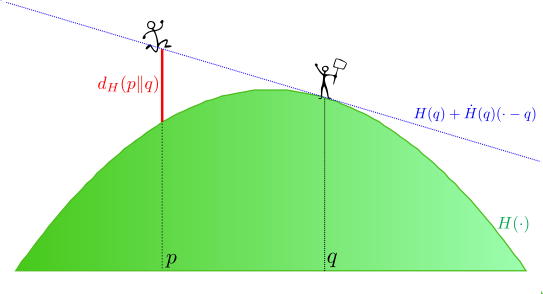
\includegraphics[width=0.8\columnwidth]{figs/embeddings/Bregman}
\end{center}
\caption[Pictorial illustration of Bregman divergences]{Pictorial illustration of Bregman divergences. Peter and Quentin are points who live on a convex hill, whose surface is described by the concave function $H(\cdot)$. Peter lives at $(p,H(p))$, Quentin at $(q,H(q))$. Because the hill is convex and they are both points, they cannot normally see each other, unless $p=q$. Anyone above the tangential line $H[q] + \dot{H}(q)(\cdot-q)$ can see Quentin, but Peter is normally below this line. If Peter wants to see Quentin, he has to jump up. The Bregman divergence $\divergence{H}{p}{q}$ measures how high Peter has to jump to see Quentin. In this example $H$ was chosen to be the Brier (quadratic) entropy, so here the divergence is symmetric, but this is not generally the case.\label{fig:Bregman}}
\end{figure}

For a more elaborate proof and discussion of Bregman divergences and scoring rules please refer to \citep{Amari2010,Dawid2007}. An intuitive explanation of Bregman divergences is given in Figure \ref{fig:Bregman}.

The information quantities introduced so far only dealt with single random variable $\X$, and comparing probability distributions over the same variable. In the following I will define information quantities that describe the relationship and dependence between more than one variable. A particularly useful quantity is the value of information, which quantifies how much useful information one random variable $Y$ holds about another one $\X$.

\begin{definition}[Generalised value of information]
	\label{def:value_of_information}
	Let $X,Y$ be random variables with joint distribution $P\in\probmeasures{\Xe\times\Ye}$. Let $\score:\Xe\times\probmeasures{\Xe}\mapsto\Reals$ be a scoring rule over the variable $X$. We define the value of information in variable $Y$ about variable $X$ with respect to the scoring rule $\score$ as
	\begin{equation}
		\information{S}{X}{Y} =  \expect{x\sim P_{X}}\score(x,P_{X})- \expect{y\sim P_{Y}} \expect{x\sim P_{X\vert Y=y}}\score(x,P_{X\vert Y=y}).
	\end{equation}
	Alternatively, we can write information in terms of the generalised entropy or divergence functions
		\begin{align}
			\information{\score}{X}{Y} &=  \genentropy{\score}{P_{X}} - \expect{y \sim P_{Y}} \genentropy{\score}{P_{X\vert Y=y}}\\
				&= \expect{y\sim P_{Y}}\divergence{S}{P_{X\vert Y=y}}{P_{X}}.
		\end{align}
\end{definition}

This quantity measures the extent to which observing the value of $Y$ is useful in forecasting variable $X$. Remarkably, this information quantity is non-symmetric. Indeed, the definition only requires a scoring rule over the variable $X$, but none over variable $Y$, so defining the value of information in $Y$ about $X$ does not even imply a definition of the value of information in $X$ about $Y$.

If the scoring rule is proper, the value of information is always non-negative. Furthermore, if the scoring rule is strictly proper, the information is zero, if and only if the two variables are independent.

\begin{theorem}
	Let $\score:\Xe\times\probmeasures{\Xe}\mapsto\Reals$ be a strictly proper scoring rule with respect to probability distributions $\probmeasures{\Xe}$, and $P\in\probmeasures{\Xe\times\Ye}$ the joint probability of variables $X$ and $Y$. Then the two statements are equivalent:
	\begin{enumerate}
		\item $\information{\score}{X}{Y} = 0$, and
		\item $\independent{X}{Y}$; the variables $X$ and $Y$ are independent.
	\end{enumerate}
	\begin{proof}
		If $X$ is independent of $Y$, then $\forall y: P_{X\vert Y=y} = P_{X}$, which implies $\forall y:  \divergence{S}{P_{X\vert Y=y}}{P_{X}}=0$, and hence $\information{\score}{X}{Y} = 0$.
		
		On the other hand, $\information{\score}{X}{Y} > 0$ implies $\exists y: \divergence{S}{P_{X\vert Y=y}}{P_{X}} > 0$, therefore by strict propriety of $\score$, $\exists y: P_X \neq P_{X\vert Y=y}$, hence $\X$ and $Y$ are dependent.
	\end{proof}
\end{theorem}

As a corollary, strictly proper scoring rules are equivalently strong in the sense that if one detects dependence between variables, than any of them will:

\begin{corollary}[Weak equivalence of strictly proper scoring rules]
	Let $\score_1,\score_2:\Xe\times\probmeasures{\Xe}\mapsto\Reals$ be two strictly proper scoring rules over $X$. $X$ and $Y$ are two random variables. Then $\information{\score_1}{X}{Y} > 0$ if and only if $\information{\score_2}{X}{Y} > 0$.
\end{corollary}

It also follows that the value of information defined by strictly proper scoring rules is weakly symmetric in the following sense:

\begin{corollary}[Weak symmetry of information]
	Let $\score_X:\Xe\times\probmeasures{\Xe}\mapsto\Reals$ be a strictly proper scoring rule over $X$ and $\score_Y:\Ye\times\probmeasures{\Ye}\mapsto\Reals$ be a strictly proper scoring rule over $Y$.  Then $\information{\score_X}{X}{Y} > 0$ if and only if $\information{\score_Y}{Y}{X} > 0$.
\end{corollary}

We can also define a conditional version of this quantity which measures how much additional information $Y$ provides about $X$ given the value of a third variable $Z$ which is also observed.

\begin{definition}[Conditional value of information]
	\label{def:conditional_value_of_information}
	Let $X,Y,Z$ be random variables with joint distribution $P\in\probmeasures{\Xe\times\Ye\times\Ze}$. Let $\score:\Xe\times\probmeasures{\Xe}\mapsto\Reals$ be a scoring rule over the variable $X$. We define the conditional value of information in variable $Y$ about variable $X$ with respect to the scoring rule $\score$ as
	\begin{equation}
		\conditionalinformation{S}{X}{Y}{Z=z} =  \expect{x\sim P_{X\vert Z=z}}\score(x,P_{X\vert Z=z})- \expect{y\sim P_{Y\vert Z=z}} \expect{x\sim P_{X\vert Y=y, Z=z}}\score(x,P_{X\vert Y=y, Z=z}).
	\end{equation}
	Alternatively, we can write information in terms of the generalised entropy or divergence functions
		\begin{align}
			\conditionalinformation{\score}{X}{Y}{Z=z} &=  \genentropy{\score}{P_{X\vert Z=z}} - \expect{y \sim P_{Y \vert Z=z}} \genentropy{\score}{P_{X\vert Y=y, Z=z}}\\
				&= \expect{y\sim P_{Y}}\divergence{S}{P_{X\vert Y=y, Z=z}}{P_{X\vert Z=z}}.
		\end{align}
\end{definition}

Just like in the case of non-conditional value of information, the definition only calls for a scoring rule over $X$, not over the other variables $X$ or $Z$. Just like the value of information was related to statistical independence, conditional value of information is related to conditional independence in the following sense.

\begin{statement}
	Let $\score:\Xe\times\probmeasures{\Xe}\mapsto\Reals$ be a strictly proper scoring rule with respect to Borel probability distributions $\probmeasures{\Xe}$, and $P\in\probmeasures{\Xe\times\Ye\times\Ze}$ the joint probability of variables $X$ and $Y$ and $Z$. Then the following two statements are equivalent:
	\begin{enumerate}
		\item $\conditionalinformation{\score}{X}{Y}{Z=z} = 0$, and
		\item $\conditionallyindependent{X}{Y}{Z=z}$; the variables $X$ and $Y$ are conditionally independent given $Z=z$.
	\end{enumerate}
\end{statement}


\section{Examples of scoring rules}

After having discussed general properties of scoring rules and information quantities based on them, let us look at particular examples of scoring rules, entropies and divergences they define. I will review three widely known scoring rules, the logarithmic, Brier (quadratic) and spherical scores. Then I present the kernel scoring rule, which is lesser known in the statistics literature. I establish the connections between the kernel scoring rule to the maximum mean discrepancy, a divergence measure that has gained popularity recently in the machine learning community over the past years \citep{Gretton2012,Sriperumbudur2008}.

Following the discussion of kernel scoring rules I define a novel scoring rule, called \emph{spherical kernel scoring rule}, examine its properties, and provide a proof that it is strictly proper. Finally, I show the connections between scoring rules and Bayesian decision theory, and explain how decision problems give rise to scoring rules and associated information quantities.

\subsection{The logarithmic score\label{sec:log_score}}

The most straightforward, and most widely used scoring rule is the logarithmic score which is of the form:
%
\begin{equation}
	\score_{log}(x,P) = - \log P(x).
\end{equation}

This score is widely used, most notably in maximum likelihood estimation of parametric models. Maximum likelihood estimation is a special case of score matching as defined in Definition \ref{def:score_matching}:
%
\begin{equation}
	\hat{\theta}_{ML} = \argmax_{\theta} \sum_{n=1}^{N} \log P(x_i \vert \theta).
\end{equation}

The associated entropy function is Shannon's entropy, also known as differential entropy for continuous distributions:
%
\begin{equation}
	\genentropy{Shannon}{P} = - \expect{x\sim P} \log P(x).
\end{equation}

The divergence function is the Kullback-Leibler (KL) divergence, which is very widely used in approximate Bayesian inference, model selection and active learning:
%
\begin{equation}
	\KL{P}{Q} = \expect{x\sim P} \log \frac{P(x)}{Q(x)}.\label{eqn:KL_divergence}
\end{equation}

The KL divergence is only well-defined when the distribution $Q$ is absolutely continuous with respect to $P$. This is a serious limitation of the KL divergence for our purposes in later chapters: If $P$ is a continuous density, then $Q$ has to be continuous as well for the KL divergence to be defined. Therefore we cannot express the KL divergence between, say, an empirical distribution of samples and a continuous distribution, as we did in Definition \ref{def:score_matching}.

A related problem is that Shannon's entropy of atomic distributions or mixed atomic and continuous distributions is either not well defined or depends only on the relative weight of the atoms but not on their locations. As we will see, information quantities based on other scoring rules remain well defined for wider classes of distributions including atomic ones.

These problems are related to a property of the logarithmic score, known as locality: The value of the scoring rule $\score(x,P)$ only depends on the value of the density function evaluated at the point $x$. This is a unique property of the logarithmic score: any strictly proper scoring rule that is local is analogous to the logarithmic score. Note, that there are weaker definitions of locality of scoring rules, which hold for scoring rules other than the logarithmic \citep{Parry2012, Dawid2012}.

\cbstart Maximum likelihood estimation, the logarithmic score and KL divergence play fundamental roles in statistics and in the field of information geometry \citep{Amari00}. KL divergence, and the associated Fisher information metric can be used to define the natural Riemannian geometry of finite-dimensional discrete probability distributions \cite{Amari00}.

The Fisher information matrix also plays a central role in the Crem\'{e}r-Rao bound \citep{Cremer99}, which expresses a lower bound for the variance of any estimator of the parameters of a statistical model. In the limit of increasing number of observations the maximum likelihood estimator achieves this lower bound, and is hence it is called assymptotically efficient. Most other scoring rules considered in this chapteres do not yield assymptotically efficient estimators \citep[see \eg][]{Varin11}. These deep connections to information geometry and the theory of statistical estimation make the logarithmic score such an important and ubiquitous example.
\cbend

The value of information becomes Shannon's mutual information, a crucial quantity in communication and channel coding \citep{Shannon1948, MacKay2002}. Shannon's mutual information has several equivalent definitions. Interestingly, it can be rewritten as the KL divergence between the joint distribution $P_{\X,Y}$ and the product of its marginals $P_{\X}P_{Y}$:
%
\begin{align}
	\information{Shannon}{X}{Y} &= \genentropy{Shannon}{X} - \expect{y \sim P_{Y}} \genentropy{Shannon}{P_{X\vert Y=y}}\\
		&= \expect{y \sim P_{Y}}\KL{P_{X\vert Y=y}}{P_X}\\
		&= \expect{y \sim P_{Y}}\left[\expect{x \sim P_{X\vert Y=y}} \log\frac{P_{X\vert Y=y}(x)}{P_X(x)} \right]\\
		&= \expect{(x,y) \sim P} \log \frac{P(x,y)}{P_{X}(x)P_{Y}(y)}\\
		&= \KL{P(x,y)}{P_{X}(x)P_{Y}(y)}.\label{eqn:mutualinfo_as_KLdivergence}
\end{align}

As a consequence, Shannon's information is symmetric. Recall, that the value of information is generally non-symmetric, 

The Shannon information in $Y$ about $X$ is the same as the Shannon information in $X$ about $Y$. This is a remarkable property of the log-score and, as we concluded in the previous section, is not generally true for value of information defined based on general scoring rules.

For completeness, I note here that some authors have generalised Shannon's mutual information along the lines of \eqref{eqn:mutualinfo_as_KLdivergence}, by replacing the KL divergence with a more general divergence $d$:
%
\begin{equation}
	\mathbb{J}_{d}(X,Y) = \mbox{d}\left[ P(x,y) \middle\| P_{X}(x)P_{Y}(y) \right].\label{eqn:mutualinfo_generalisations}
\end{equation}

Examples of information functionals defined this way are described in \citep{Poczos2011}.
On one hand, an information functional like $\mathbb{J}$ has several nice properties, most notably that it is always symmetric. On the other hand, in the general case we loose the intuitive meaning of information as ``the extent to which observing the value of one variable is useful for predicting the value of the other one''. Furthermore, if we wanted to use a divergence function corresponding to a scoring rule, the scoring rule should be defined over the joint space $\Xe\times\Ye$, which is often not desired.

\subsection{The pseudo-likelihood\label{sec:pseudolikelihood}}

The idea of maximum pseudo-likelihood estimation was introduced originally by \citet{Besag1977} to estimate parameters of Gaussian random fields. Later it was popularised in the context of parameter estimation in general Markov random fields \citep{Comets1992} and in Boltzmann machines \citep{Hyvarinen2006}. The pseudo-likelihood is particularly useful for estimating parameters of statistical models with intractable normalisation constants.

\begin{equation}
	\score_{\mbox{pseudo}}(x,P) = - \sum_{d=1}^{D} \log P(x_d\vert x_{\neg d}),
\end{equation}
where $x_d$ denotes the $d^{\mbox{th}}$ component of the vector $\x$ and$x_{\neg d}$ denotes the vector composed of all components of $x$ other than the $d^{\mbox{th}}$ component $x_d$.

In the pseudo-likelihood each of the terms is the conditional probability over one variable conditioned on all the remaining variables. Such quantities can be computed by marginalising a single variable at a time, therefore by computing a one dimensional integral or sum:
%
\begin{equation}
	p(x_d\vert x_{\neg d}) = \frac{P(x)}{\int P(X_d=y,x_{\neg d}) dy} = \frac{C \cdot P(x)}{\int C \cdot P(X_d=y,x_{\neg d}) dy}.
\end{equation}
%
This can be computed even if the joint probability of all variables $P$ is known only up to a multiplicative constant $C$, which is very often the case.

Take the Boltzmann distribution with parameters $W$ and $b$ as an example. 
%
\begin{equation}
	P(\x) = \frac{1}{Z}\exp(x^{T}Wx + b^{T}x), x\in\{0,1\}^D,
\end{equation}
%
where $Z = \sum_{x\in\{0,1\}^D}\exp(x^{T}Wx + b^{T}x)$ is the partition function or normalisation constant that is analytically intractable to compute in the general case. On the other hand, the conditional distribution of a single component of $x$ conditioned on the rest is easy to compute as follows:
%
\begin{align}
	P(x_d\vert x_{\neg d}, W, b) &= \frac{p(x)}{\int p(x_d=y,x_{\neg d}) dy}\\
		&= \frac{\frac{1}{Z}\exp(x^{T}Wx + b^{T}x)}{\sum_{x_d\in\{0,1\}}\frac{1}{Z}\exp(x^{T}Wx + b^{T}x)}\\
		&= \frac{\exp(x^{T}Wx + b^{T}x)}{\sum_{x_d\in\{0,1\}}\exp(x^{T}Wx + b^{T}x)}\\
		&= \frac{\exp\left( x_d \left( W_{d,d} + 2 W_{d,\neg d}^{T}x_{\neg d} + b_d \right)\right)}{\exp( W_{d,d} + 2 W_{d,\neg d}^{T}x_{\neg d} + b_{d}) + 1}.
\end{align}

The pseudo-likelihood thus becomes a sum of easy-to-compute sigmoidal terms. These sigmoidal terms, and their derivatives with respect to parameters $W$ and $b$ can be computed in polynomial time, allowing for fast estimation algorithms. \citet{Hyvarinen2006} showed that pseudo-likelihood estimation -- score matching with the pseudo-likelihood score -- is consistent for fully visible Boltzmann machines. \citet{Besag1977,Comets1992} showed similar results for Markov random fields.

The difference between the pseudo-likelihood score and the log score becomes more apparent when rewriting the log score by the chain rule of joint probabilities:
%
\begin{equation}
	\score_{\mbox{log}}(x,p) = - \log P(x) =  - \sum_{d=1}^{D} \log P(x_d\vert x_{1:d-1}).
\end{equation}

Here the $d^{\mbox{th}}$ term is a probability conditioned on $d-1$ variables. Computing the $d^{\mbox{th}}$ term therefore would require $D-d$ dimensional integral in the general case. The pseudo-likelihood makes computations more efficient by conditioning on more variables than needed by the chain rule, therefore requiring lower dimensional integrals.

\citet{Csiszar2004} showed that pseudo-likelihood score is strictly proper for strictly positive distributions. Moreover, for always positive distributions the following generalisation of the pseudo-likelihood is also a strictly proper scoring rule \citep*{Dawid2012}:
%
\begin{equation}
	\score_{\mbox{DLP12}}(x,P) = - \sum_{d=1}^{D} \score_d\left(x_d, P_{X_d \vert X_{\neg d}=x_{\neg d}}\right),
\end{equation}
%
where $\score_d$ are strictly proper scoring rules for each dimension.

\cbstart

\subsection{Composite likelihoods\label{sec:composite_likelihood}}

Composite likelihoods were introduced by \citet{Lindsay88}, and they can be thought of as a further generalisation of the pseudo-likelihood. The main motivation behind composite likelihoods is to construct estimators which do not require the evaluation of intractable marginalisation constants which makes logarithmic score infeasible in many practical applications. Instead, composite likelihood scores are constructed as sums of lower dimensional marginal or conditional logarithmic scores which are feasible to compute.

In their most general form, composite likelihood can be described as follows. Let $P\in\probmeasures{\Xe}$ a probability distribution over the variable $X\in\Xe$. Let $\mathcal{A}_1,\cdot,\mathcal{A}_K\subseteq\Xe$ denote measurable events, $w_1,\ldots,w_K$ positive weights. The composite likelihood is a scoring rule of the following form:
%
\begin{equation}
	\score_{CL}(x,P) = \sum_{k=1}^{K} w_k \cdot \log P(x\in\mathcal{A}_k).\label{eqn:composite_likelihood}
\end{equation}

Because each component is strictly proper, composite likelihoods are proper -- albeit not always strictly proper -- scoring rules. By specifying the sets of events $\mathcal{A}_k$ and corresponding weights, this class generalises the log score, the pseudo-likelihood, as well as other interesting cases. This construction has been referred to by different names in the literature, including composite likelihood \citep{Lindsay88,Varin11}, pseudo-likelihood \citep{Molenberghs05}, qausi-likelihood \citep{Hjort94} and approximate likelihood \citep{Stein04}. Here I adopt the terminology of \citet{Lindsay88}, and reserve the term pseudo-likelihood to refer to the special case covered in the previous section, originally introduced by \citet{Besag1977}.

A review by \citet{Varin11} divides composite likelihood methods into two main branches based on whether they are composed of marginal or conditional probabilities.

\emph{Composite conditional likelihood} methods construct proper scoring rules out of sets of conditional distributions. Besag's pseudolikelihood of Section \ref{sec:pseudolikelihood} is the best known example of this family. \citet{Molenberghs05} considered the following composite likelihood composed of pairwise conditional distributions:
%
\begin{equation}
	\score_{MV05}(x,P) = \sum_{d=1}^{D}\sum_{\substack{e=1\\e\neq d}}^{D} \log P(x_d\vert x_e).
\end{equation}
%
A further example of composite conditional likelihoods is the order-$m$ likelihood estimation technique introduced by \citet{Azzalini83}. This approach works by omitting long-range spatial dependencies in stationary stochastic processes.

In \emph{composite marginal likelihood} methods the scoring rule is constructed from marginal distributions. The simplest of such scoring rules is the \emph{independence likelihood} \citep{Chandler07} of the following form:
%
\begin{equation}
	\score_{independence}(x,P) = \sum_{d=1}^{D} \log P(x_d).
\end{equation}
%
It is clear that the independence likelihood is strictly proper only with respect to distributions that factorise over dimensions. Thus, it only permits unbiased estimation of marginal parameters. More powerful scoring rules attempt to better capture dependencies by considering higher order marginals, such as the pairwise likelihood of \citet{Cox04}:
%
\begin{equation}
	\score_{pairwise}(x,P) = \sum_{d=1}^{D-1} \sum_{e=d+1}^{D} \log P(x_d,x_e).
\end{equation}
%
Further special cases are reviewed in \citep{Varin11}.

A central object of interest in the topic of composite likelihoods is the \emph{sandwich information matrix}, a generalisation of the Fisher information matrix. This matrix is crucial in characterising the convergence properties of statistical estimators based on composite likelihoods. For example, a composite likelihood is strictly proper scoring rule, whenever the corresponding sandwich matrix is of full rank. For definitions, and further details the reader is referred to \citep{Lindsay88} or \citep{Varin11}.

Composite likelihood scores can be generalised further -- along the lines of \citep{Dawid2012} -- by replacing the component likelihoods by arbitrary strictly proper scoring rules. It is unclear wether such generlisations provide any practical benefit, especially as the established theoretical framework based on the sandwich information matrix would not extend to this case.

\cbend

\subsection{The quadratic Brier score\label{sec:Brier_score}}

Another widely used scoring rule is the so-called \emph{Brier score} or quadratic score, originally introduced in \citep{Brier1950}. It was first applied to evaluating probabilistic weather forecasts and it is still widely used in meteorology \citep{Ferro2007} as well as in medicine \citep{Spiegelhalter2006} and epidemiology \citep{Redelmeier1991}. It is also related to the root mean squared error (RMSE) of probabilistic binary classifiers, which is a commonly used loss function for training neural networks \citep{Rumelhart1988}.

We will define the Brier score in terms of the $L^2$ norm of probability distributions, which we define as
%
\begin{equation}
	\customnorm{P}{2} \defeq \sqrt{\expect{x \sim P} P(x)}.
\end{equation}

The above definition, albeit slightly informal, is well defined and finite for most classes of probability distributions we are concerned with. For continuous distributions, $P(x)$ denotes the probability density, for discrete distributions $P(x)$ denotes the probability of outcome $x$. Similarly, one can define the scalar product between two distributions as follows:
%
\begin{equation}
	\scalar{P}{Q} \defeq \sqrt{\expect{x \sim P} Q(x)}.
\end{equation}

Using these definitions we can define the Brier score as follows:
%
\begin{align}
	\score_{Brier}(x,P) &= \customnorm{P - \delta_{x}}{2}^2\\
		&= \customnorm{P}{2}^{2} - 2P(x)  + 1\\
		&= \expect{x' \sim P} P(x') - 2P(x) + 1,
\end{align}
%
where $\delta_{x}$ is the discrete or continuous Dirac measure concentrated at the observed point $\x$.

The score gives rise to the following entropy function:
%
\begin{align}
	\genentropy{Brier}{P} &= \expect{x \sim P}\left[\expect{x' \sim P} P(x') - 2P(x) + 1\right]\\
		&= 1 -\expect{x \sim P} P(x)\\
		&= 1 - \customnorm{P}{2}^2.
\end{align}

For discrete distributions when $\dim \Xe = D$, the quadratic entropy function is bounded. It's maximum value is attained when $P$ is the $D$ dimensional uniform distribution: then it equals $1 - \sum_{d=1}^{D}\frac{1}{D^2} = 1 - \frac{1}{D}$. The upper bound is $1$ if $\dim \Xe = \infty$. The entropy function is also non-negative for discrete distributions, with $\genentropy{Brier}{P}=0$ only for atomic distributions $P=\delta_{x_0}$.

In uncountable domains, just like Shannon's entropy, The entropy function becomes unbounded from below. For atomic distributions it takes value $-\infty$. Unlike Shannon's entropy, it is always bounded from above.

The Brier divergence function becomes the squared norm of the difference between the distributions:
%
\begin{align}
	\divergence{Brier}{P}{Q} &= \expect{x \sim P}\left[\customnorm{Q}{2}^2 - 2Q(x) + 1\right] - \genentropy{Brier}{P} \\
		&= \customnorm{Q}{2}^2 -2 \expect{x \sim P} Q(x) + \customnorm{P}{2}^2 \\
		&= \customnorm{Q}{2}^2 - 2\scalar{P}{Q} + \customnorm{P}{2}^2\\
		&= \customnorm{P-Q}{2}^2. \label{eqn:Brier_divergence}
\end{align}

\cbstart
Interestingly, the Brier divergence is symmetric, and it is analogous to the squared Euclidean distance. For distributions with continuous densities, the Brier divergence is also known as Integrated Squared Error (ISE). This distance metric has been used for decades in studying convergence properties of nonparametric density estimates, such as Parzen window estimates \citep{Parzen62}. In more modern work it has also been applied as a direct optimisation criterion for fitting parametric density models \citep[see \eg][]{Scott99,Mukherjee99,Girolami03}.
\cbend

The value of information under the Brier score becomes the following straightforward quantity:
%
\begin{align}
	\information{Brier}{X}{Y} &= \expect{y \sim P_{Y}} \customnorm{P_X - P_{X\vert Y=y}}{2}^2.
\end{align}

\subsection{Spherical scoring rules}

Another example of strictly proper scoring rules, introduced in \citep{Good1971}, is the spherical scoring rule \citep{Dawid2007,Dawid2012}. The spherical score is defined as follows:
%
\begin{align}
	\score_{spherical}(x,P) &= 1 -\frac{P(x)}{\customnorm{P}{2}}.
\end{align}

This gives rise to the following entropy and divergence functionals:
%
\begin{align}
	\genentropy{spherical}{P} &= 1 -\expect{x \sim P}\frac{P(x)}{\customnorm{P}{2}}\\
		&= 1 -\customnorm{P}{2},\\
	\divergence{spherical}{P}{Q} &= -\expect{x \sim P}\frac{Q(x)}{\customnorm{Q}{2}} + \customnorm{P}{2}\\
		&= \customnorm{P}{2} - \frac{\scalar{Q}{P}}{\customnorm{Q}{2}}\\
		&= \customnorm{P}{2}\left( 1 - \cos(P,Q) \right),
\end{align}
%
where $\cos(P,Q) = \frac{\scalar{P}{Q}}{\customnorm{P}{2}\customnorm{Q}{2}}$ is the cosine similarity between distributions $P$ and $Q$.

An interesting property of the spherical score is that it is agnostic to scaling of $P$. That is $\score_{spherical}(x,c\cdot P) = \score_{spherical}(x,P) $. Similarly, $\divergence{spherical}{P}{c\cdot Q} = \divergence{spherical}{P}{Q}$ and $\divergence{spherical}{c\cdot P}{Q} = c \cdot \divergence{spherical}{P}{Q}$. This means that when approximating a fixed distribution $P$ by $Q$ via minimising $\divergence{spherical}{P}{Q}$ we only need to know $P$ and $Q$ up to a normalising constant.

The value of information under the spherical score is
%
\begin{align}
	\information{spherical}{X}{Y} &= \customnorm{P_X}{2}\expect{y \sim P_{Y}} \left( 1 - \cos(P_X,P_{X\vert Y=y}) \right).
\end{align}

\citet{Gneiting2007} and \citet{Jose2008} also introduce generalisations of the spherical score, where the $L_2$ norm is replaced by a general $L_\gamma$ norm:
%
\begin{align}
	\genentropy{\gamma,pseudospherical}{P} &= -\customnorm{P}{\gamma}.
\end{align}

\subsection{The kernel scoring rule\label{sec:kernel_score}}

The kernel scoring rule first appeared in the statistics literature in \citep{Eaton1996}, although the name \emph{kernel scoring rule} was only used in more recent references \citep{Dawid1994,Dawid2007,Gneiting2007}.

Independently, a related concept, derived from different first principles, has become known in the machine learning community as \emph{maximum mean discrepancy} (MMD, \citep{Sriperumbudur2008}). As we will see, MMD is closely related to the kernel scoring rule. MMD has been adopted in a variety of modern applications in machine learning and statistics, including two sample tests \citep{Gretton2012}, kernel moment matching \citep{Song2008}, embedding of probability distributions \citep{Smola2007} and the kernel-based message passing \citep{Fukumizu2010}.

MMD measures the divergence or distance between two distributions, $P$ and $Q$. It belongs to a rich class of divergences called integral probability metrics \citep{Sriperumbudur2009}, which define the distance between  $P$ and $Q$, with respect to a class of integrand functions $\mathcal{F}$ as follows:
%
\begin{align}
	\divergence{\Fe}{P}{Q} = \sup_{f\in\Fe}\left\vert \expect{x\sim P} f(x) - \expect{x\sim Q} f(x) \right\vert^2.
\end{align}
	
Intuitively, if two distributions are close in the integral probability metric sense, then no matter which function $f$ we choose from the function class $\mathcal{F}$, the difference between the expectation of $f$ under $P$ and $Q$ should be small. This class of divergences include the Wasserstein distance \citep{Barrio1999}, the Dudley metric \citep{Dudley1974} and MMD, which differ only in their choice of the function class $\Fe$.

A particularly interesting case is when the function class $\Fe$ is functions of unit norm from a reproducing kernel Hilbert space (RKHS) $\He$. In this case, the MMD between two distributions can be conveniently expressed using expectations of the associated kernel $k(x, x')$ only \citep{Sriperumbudur2008}:
%
\begin{align}
\mbox{MMD}^2\left(P,Q\right) &= \sup_{\substack{f\in\He\\\Hnorm{f}=1}}\left( \expect{x\sim P} f(x) - \expect{x\sim Q} f(x) \right)^2\label{eqn:rkhs-mmd}\\
	&=  \sup_{\substack{f\in\He\\\Hnorm{f}=1}}\left\vert \expect{x\sim P}\scalar{f}{k(\cdot,x)} - \expect{x\sim Q} \scalar{f}{k(\cdot,x)} \right\vert^2\label{eqn:MMD_reproducing_property}\\
	&=  \sup_{\substack{f\in\He\\\Hnorm{f}=1}}\left\vert \scalar{f}{\expect{x\sim P} k(\cdot,x) - \expect{x\sim Q} k(\cdot,x)}\right\vert^2\label{eqn:MMD_linearity_of_expectation}\\
	&=  \sup_{\substack{f\in\He\\\Hnorm{f}=1}}\scalar{f}{\mu_{P} - \mu_{Q}}^2\\
	&=  \Hnorm{\mu_{P} - \mu_{Q}}^2\label{eqn:MMD_Cauchy_Schwartz}\\
	&=  \expect{x,x'\sim P} k(x,x')	- 2 \expect{x\sim P}\expect{x'\sim Q} k(x,x') + \expect{x,x'\sim Q} k(x,x').\label{eqn:rkhs-mmd-lastline}
\end{align}

In the derivation above we exploited the reproducing property of the kernel to arrive at \eqref{eqn:MMD_reproducing_property} and the linearity of expectation to obtain \eqref{eqn:MMD_linearity_of_expectation}. Step \eqref{eqn:MMD_Cauchy_Schwartz} holds because of the Cauchy-Schwartz inequality. $\mu_P(\cdot) = \expect{x\sim P} k(\cdot,x)$ is called the mean element or RKHS-embedding of the probability distribution $P$ \citep{Smola2007}. The MMD metric is analogous to the Euclidean distance between the mean elements of the two distributions.

The most interesting kernels for the purposes of Hilbert-space embedding of distributions are those called \emph{characteristic} \citep{Sriperumbudur2008}. If the kernel $k$ is characteristic, the mapping from Borel probability measures to mean elements is injective, that is $\mu_P = \mu_Q \iff P = Q$. This also means that for characteristic Hilbert spaces $\divergence{k}{P}{Q} = 0 \iff Q=P$ holds. This is analogous to the strictly proper property of scoring rules and divergences as in Definition \ref{def:strictly_proper}.

The mean embedding $\mu_P$ can be thought of as a generalisation of characteristic functions \citep[see \eg][]{Ord1999}. The characteristic function of a probability distribution $P$ with density $p$ over the real line is defined as follows:
%
\begin{equation}
	\phi_p(t) = \E{x\sim p}{e^{ i t x}} = \int e^{i t x} p(x) dx,
\end{equation}
%
where $i$ is the imaginary number $i=\sqrt{-1}$.

The characteristic function is known to uniquely characterise any Borel probability measure on the real line. Indeed, it corresponds to an RKHS-embedding with the Fourier kernel $k_{Fourier}(x,y) = \exp(ixy)$, which is an example of characteristic kernels. Note, that the final formula \eqref{eqn:rkhs-mmd-lastline} assumed a real valued kernel function, therefore it is not valid for the special case of the Fourier kernel. Other, practically more relevant examples of characteristic kernels include the squared exponential, and the Laplacian kernels \citep[see \eg][]{Rasmussen2006}. As a counterexample, polynomial kernels, and in general kernels corresponding to finite dimensional Hilbert spaces are not characteristic \citep{Sriperumbudur2008}.

The maximum mean discrepancy with characteristic kernels has been applied in various contexts in machine learning. One of the first of these recent applications were two-sample tests. In two-sample testing one is provided i.\,i.\,d.\ samples from two distributions, and one has to determine whether the two distributions are the same or not. \citet{Gretton2012} developed and analysed efficient empirical methods based on the MMD for this problem.

Herding \citep{welling2009herding} and its generalisation kernel herding \citep{Chen2010} have been shown to minimise MMD between a target distribution and the empirical distribution of pseudo-samples. This method is an example of quasi-Monte Carlo methods that are examined in Chapter \ref{sec:approximate_inference}. Lastly, in kernel moment matching \citep{Song2008} MMD is used for density estimation: parameters of a parametric density model are set by minimising MMD from the empirical distribution of data.

The squared MMD in fact conforms to our definition of a generalised divergence in equation \eqref{eqn:def_divergence}, and corresponds to the following scoring rule:
%
\begin{align}
	\score_{k}(x,P) &\defeq k(x,x) - 2 \expect{x'\sim P} k(x,x') + \expect{x',x''\sim P}k(x',x'') \label{eqn:kernel_scoring_rule}\\
		&=  \sup_{\substack{f\in\He\\\Hnorm{f}=1}}\left( f(x)- \expect{x\sim P} f(x) \right)^2.
\end{align}

The equivalence can be seen by applying Definition \ref{def:generalised_divergence} of the generalised divergence:
%
\begin{align}
	\divergence{k}{P}{Q} &\defeq \expect{x\sim P} \score_{k}(x,Q) - \expect{x\sim P} \score_{k}(x,P)\\
		&= \expect{x\sim P} k(x,x) - 2 \expect{x\sim P}\expect{x'\sim Q} k(x,x') + \expect{x',x''\sim Q}k(x',x'')\\
		&\ \ \ \,- \expect{x\sim P} k(x,x) + 2 \expect{x,x'\sim P} k(x,x') - \expect{x',x''\sim P}k(x',x'') \\
		&= \expect{x',x''\sim P}k(x',x'') - 2 \expect{x\sim P}\expect{x'\sim Q} k(x,x') + \expect{x',x''\sim Q}k(x',x'')\\
		&= \mbox{MMD}^2\left(P,Q\right).
\end{align}

The scoring rule in Equation \eqref{eqn:kernel_scoring_rule} is equivalent to the \emph{kernel scoring rule} introduced originally by \citet{Eaton1982}. The term kernel score was later coined by \citet{Dawid2007}. Further references to this scoring rule can be found in \citep{Eaton1996,Gneiting2007}. The original definitions differed from the formula by a factor of two, and they did not have the leading $k(x,x)$ term. These differences do not make any practical effect: scoring rules that are equal up to scaling and an additive term that depends only on $x$ but not on the distribution $P$ give rise to exactly the same generalised entropy and divergence functionals, and are hence equivalent \citep{Dawid2007}. Also, the statistics community defined the scores in terms of negative definite kernels, rather than positive definite ones which is the common convention in machine learning.

It has also been pointed out that the Brier (quadratic) score is a special case of the kernel score when the kernel is chosen to be the trivial $k(x,x') = \delta(x - x')$, where $\delta$ is the Dirac delta function \citep{Dawid2007}.
\cbstart
Thus, methods that minimise the integrated squares error -- \ie the quadratic Brier divergence in Eqn.\ \eqref{eqn:Brier_divergence} -- can also be considered as special cases of kernel moment matching \citep{Scott99,Girolami03,Mukherjee99}.
\cbend

To my knowledge the connection between kernel scores in statistics and maximum mean discrepancy has not been established before. This interpretation allows one to uncover previously unknown connections between existing machine learning methods and to provide a solid theoretical framework for understanding and generalising them. For example, novel asymptotic analysis may established using generalisations of the Fisher information matrix or the sandwitch information matrix.

Depending on the choice of kernel, the kernel score can be strictly proper. \citep{Gneiting2007} provide a proof of the propriety of the kernel scoring rule with respect to all Borel probability measures, given that the expectation $\expect{x,x'\sim P} k(x,x')$ is finite. Using the theory developed to study properties of MMD and characteristic kernels we can also see that the scoring rule is strictly proper whenever the kernel is characteristic \citep{Sriperumbudur2008}. \citet{Gneiting2007} showed that many examples of scoring rules, among them the Brier score (see section \ref{sec:Brier_score}), can be interpreted as special cases of the kernel scoring rule.

The generalised entropy defined by this scoring rule becomes:
%
\begin{align}
	\genentropy{k}{P} &= \expect{x\sim P} \score_{k}(x,P) \\
		&= \expect{x\sim P} k(x,x) - 2 \expect{x,x'\sim P} k(x,x') + \expect{x',x''\sim P}k(x',x'')\\
		&= \expect{x\sim P} k(x,x) - \expect{x,x'\sim P} k(x,x').
\end{align}

The entropy function is concave for all positive definite kernels $k$ and strictly concave whenever the kernel is characteristic. Importantly, it has several favourable properties in comparison to Shannon's entropy.

Firstly, if we assume that the kernel $k$ is bounded, then the entropy functional is also bounded. If we further assume that the kernel satisfies $\forall x,y: k(x,x)\geq k(x,y)$, then the entropy is also non-negative. Thus, in most practical cases the entropy functional is bounded both from above and below. Irrespective of kernel choice, the entropy is exactly zero for delta distributions, that is when the distribution $P$ is concentrated on a single point. If the kernel satisfies the strict inequality $\forall x,y: k(x,x) > k(x,y)$, the entropy is strictly positive for all other probability distributions.

Secondly, the entropy can be computed for any distribution that one can compute expectations over. This means that any probability distribution, and indeed any Borel measure, has a well-defined entropy of this form. This is not true for the Shannon's differential entropy, where the entropy of atomic distributions or mixtures of atomic and continuous distributions is not defined. This property is useful in applications such as quasi-Monte Carlo as discussed in Chapter \ref{sec:approximate_inference}.

Thirdly, the entropy function has the kernel $k$ as a free parameter, which is mixed blessing. On one hand, this provides extra flexibility: even if we commit to a particular family of kernels, like the square exponential, we can fine-tune the entropy function and corresponding divergence to our needs by adjusting parameters, such as the length-scale parameter \citep{Song2008}. On the other hand there is no principled, general way of choosing the kernel or its parameters if we are unsure what it should be. 

We can use the generalised entropy and divergence defined by the kernel scoring rule to define the value of information a random variable provides about another one:
%
\begin{align}
	\information{k}{X}{Y} &= \expect{y\sim P_{Y}} \divergence{k}{P_{X}}{P_{X\vert Y=y}}\\
		&=  \expect{y\sim P_{Y}} \Hnorm{ \mu_{X \vert Y=y} - \mu_X }^2 \label{eqn:kernel_information}\\
		&= k(P_{X},P_{X}) - 2*\expect{y\sim P_{Y}}k(P_{X},P_{X\vert Y=y}) + \expect{y\sim P_{Y}} k(P_{X\vert Y=y},P_{X\vert Y=y})\\
		&= \expect{y\sim P_{Y}} \expect{P_{x_1,x_2 \sim P_{X\vert Y=y}}}k(x_1,x_2) - \expect{x_1,x_2\sim P_{X}}k(x_1,x_2),
\end{align}
%
where I used the shorthand notation $k(P,Q)=\expect{x\sim P,x'\sim Q}k(x,x')$.

To my knowledge, this kernel-based measure of information has not been defined or used in the machine learning or statistics literature before. It is interesting to contrast this to other kernel measures of dependence developed recently in statistics, which are largely based on the cross-covariance operator between Hilbert space embeddings of the two distributions.

\begin{definition}[kernel Cross-covariance operator]
	Let $X$ and $Y$ be two random variables with joint distribution $P\in\probmeasures{\Xe\times\Ye}$, and marginals $P_X$ and $P_Y$. Let $k_{\Xe}:\Xe\times\Xe\mapsto\Complex$ and $k_{\Ye}:\Ye\times\Ye\mapsto\Complex$ be positive definite kernels with associated reproducing kernel Hilbert spaces $\He_\Xe$ and $\He_\Ye$, respectively. Let us define the kernel cross-covariance operator $C_{XY}$ between $X$ and $Y$ so that for all $f\in\He_\Xe$ and $g\in\He_\Ye$
	%
	\begin{equation}
		\scalar{f}{C_{XY}g}_{\He_\Xe} = \expect{(x,y) \sim P} \left( f(x) - \expect{x'\sim P_X} f(x')\right) \left( g(y) - \expect{y' \sim P_Y} g(y')\right).
	\end{equation}
\end{definition}

Based on the cross-covariance operator, one can define various measures of dependence and information. Here I only define the simplest one, the constrained covariance, or COCO:

\begin{definition}[COCO, see \citep{Gretton2005COCO}]
	In the same notation as above let us define define the constrained covariance between $X$ and $Y$, $COCO_{XY}$, as
	%
	\begin{equation}
		COCO_{XY}=\sup_{\substack{f\in\He_\Xe, g\in\He_\Ye \\\customnorm{f}{\He_\Xe}=1,\customnorm{g}{\He_\Ye}=1}} \cov{(x,y)\sim P}{f(x)}{g(y)}.
	\end{equation}
	%
	It can be shown that, $COCO$ is the matrix norm of the cross-covariance operator:
	%
	\begin{equation}
		COCO_{XY} = \customnorm{C_{XY}}{2},
	\end{equation}
	%
	where $\customnorm{\cdot}{2}$ denotes the spectral norm, that is the modulus of largest singular value \citep{Gretton2005COCO}.
\end{definition}

A more robust measure of dependence, the Hilbert Schmidt Information Criterion (HSIC) uses the Hilbert-Schmidt norm of the cross-covariance operator\citep{Gretton2005HSIC}. Kernel measures of dependence like COCO and HSIC have several useful properties. They are symmetric, and can be effectively estimated from empirical data \citep{Gretton2005HSIC}.

However, as with generalisations of Shannon's information in Eqn.\ \eqref{eqn:mutualinfo_generalisations}, COCO and its variants do not have an interpretation as ``the extent to which knowing $Y$ is useful for predicting $X$''. Also, they require a kernel to be defined over both $\Xe$ and $\Ye$, and properties of the functional depend on both choices of kernels. In contrast \eqref{eqn:kernel_information} only requires a single kernel over $\Xe$.

Interestingly, the kernel value of information $\information{k}{X}{Y}$ that I introduced based on the kernel score can also be interpreted in terms of a linear operator in the Hilbert space. I am not aware of any previous use of this operator before, and in referencing it I will use the name diversity operator.

\begin{definition}[Diversity operator]
Given two random variables $X$ and $Y$ with joint distribution $P$, and a positive definite kernel $k:\Xe\times\Xe\mapsto\Complex$ with associated Hilbert space $\He$, let us define the \emph{diversity operator} of Y over X, $D_{X\vert Y}:\He\mapsto\He$ such that for all $f,g\in\He$
%
\begin{align}
	\scalar{f}{D_{X\vert Y}g}_{\He} = \cov{y\sim P_Y}{\expect{X\vert Y=y} f}{\expect{X\vert Y=y} g}.
\end{align}
%
Consequently for all $f\in\He$
%
\begin{align}
	\scalar{f}{D_{X\vert Y}f}_{\He} = \var{y\sim P_Y} \left[ \expect{x\sim P_{X\vert Y=y}} f(x) \right].
\end{align}
\end{definition}

Equivalently, the operator can be defined in terms of mean elements or Hilbert-space embedding of the conditional and marginal distributions as follows:

\begin{statement}[Alternative definition of $D_{X\vert Y}$]
$D_{X\vert Y}$ admits the following equivalent definition
%
\begin{align}
	D_{X\vert Y} = \expect{y\sim P_Y} \left(\mu_{X\vert Y=y} - \mu_{X}\right) \otimes \left(\mu_{X\vert Y=y}  - \mu_{X} \right),
\end{align}
%
where $\otimes$ denotes tensor product, such that $\forall f,g,h\in\He: (f\otimes g)h = \scalar{g}{h}f$.

\begin{proof}
Let $f,g\in\He$, then
%
\begin{align}
	&\scalar{f}{ \left(\expect{y\sim P_Y}\left(\mu_{X\vert Y=y} - \mu_{X}\right) \otimes \left(\mu_{X\vert Y=y}  - \mu_{X} \right)\right) g}\\
	=&\expect{y\sim P_Y}\scalar{f}{ \left(\left(\mu_{X\vert Y=y} - \mu_{X}\right) \otimes \left(\mu_{X\vert Y=y}  - \mu_{X} \right)\right) g}\\
	=& \scalar{f}{\left(\mu_{X\vert Y=y} - \mu_{X}\right)}\scalar{g}{\left(\mu_{X\vert Y=y} - \mu_{X}\right)}\\
	=& \scalar{f}{\left(\expect{x\sim P_{X\vert Y=y}}k(\cdot,x) - \expect{x\sim P_X}k(\cdot,x)\right)}\scalar{g}{\left(\expect{x\sim P_{X\vert Y=y}}k(\cdot,x) - \expect{x\sim P_X}k(\cdot,x)\right)}\\
	=& \expect{y\sim P_Y} \left(\expect{X\vert Y=y} f(x) - \expect{x\sim P_X}f(x)\right)\left(\expect{X\vert Y=y} g(x) - \expect{x\sim P_X}g(x)\right)\label{eqn:diversity_operator_linearity_of_expectation}\\
	=& \cov{y\sim P_Y}{\expect{X\vert Y=y} f}{\expect{X\vert Y=y} g}\\
	=& \scalar{f}{D_{X\vert Y}g}_{\He},
\end{align}
%
where we used the linearity of expectation and the reproducing property of the kernel to obtain step \eqref{eqn:diversity_operator_linearity_of_expectation}.
\end{proof}
\end{statement}

Using this alternative definition it is easy to see that the kernel value of information as defined in Eqn.\ \eqref{eqn:kernel_information} can be expressed as the trace of the diversity operator (which in turn is the same as the Hilbert-Schmidt norm of the square-root of the operator):
%
\begin{align}
	\information{k}{X}{Y} &= \expect{y \sim P_{Y}} \customnorm{\mu_X - \mu_{X\vert Y=y}}{2}^2\\
		&= \expect{y \sim P_{Y}} \trace{\scalar{\mu_X - \mu_{X\vert Y=y}}{\mu_X - \mu_{X\vert Y=y}}}\\
		&= \expect{y \sim P_{Y}} \trace{ ( \mu_X - \mu_{X\vert Y=y}) \otimes (\mu_X - \mu_{X\vert Y=y})}\\
		&= \trace{ \expect{y \sim P_{Y}} ( \mu_X - \mu_{X\vert Y=y}) \otimes (\mu_X - \mu_{X\vert Y=y})} \\
		&= \trace{I_{X\vert Y}}\\
		&= \customnorm{I_{X\vert Y}^{\nicefrac{1}{2}}}{HS}.
\end{align}

It would be interesting future direction to investigate whether this information criterion has any connections to COCO and HSIC, or indeed if it inherits any of their useful properties.

\subsection{The spherical kernel score\label{sec:spherical_kernel_score}}

Seeing how the Brier score is a special case of the kernel scoring rule, one might wonder whether the spherical scoring rule has a similar generalisation. It turns out it does, and it gives rise to a very intuitive divergence. Consider the following scoring rule
%
\begin{align}
	\score_{k,spherical}(x,P) &\defeq \Hnorm{\mu_{\delta_x}} - \frac{\mu_P(x)}{\Hnorm{\mu_P}} \label{eqn:spherical_kernel_score}\\
			& = \Hnorm{\mu_{\delta_x}}\left(1 - \cos(\mu_{\delta_x},\mu_{P})\right)\\
		& =\sqrt{k(x,x)} - \frac{\expect{x'\sim P}k(x,x')}{\sqrt{\expect{x,x'\sim P}k(x,x')}}.
\end{align}

The scoring rule gives rise to the following entropy functional:
%
\begin{align}
	\genentropy{k,spherical}{P} & = \expect{x\sim P}\Hnorm{\mu_{\delta_x}} - \Hnorm{\mu_P}\\
		& = \expect{x\sim P}\sqrt{k(x,x)} - \sqrt{\expect{x,x'\sim P}k(x,x')}.
\end{align}
%
Whenever $k(x,x)=c$ this entropy is non-negative, and bounded from above. For characteristic kernels it is only zero for delta distributions.

The scoring rule leads to the following divergence:
%
\begin{align}
	\divergence{k,spherical}{P}{Q} &= - \expect{x\sim Q}\frac{\mu_P}{\Hnorm{\mu_P}} + \Hnorm{\mu_P}\\
		&= \Hnorm{\mu_P} \left( 1 - \cos(\mu_P, \mu_Q)\right)\\
		&= \sqrt{\expect{x,x'\sim P}k(x,x')} - \frac{\expect{x\sim P}\expect{x'\sim Q}k(x,x')}{\sqrt{\expect{x,x'\sim Q}k(x,x')}}. \label{eqn:spherical_kernel_divergence}
\end{align}

Unlike MMD and $\divergence{k}{\cdot}{\cdot}$, this divergence is asymmetric because of the leading $\Hnorm{\mu_P}$ factor. Also, just like the spherical score, it is agnostic to scaling of $Q$, that is
%
\begin{equation}
	\divergence{k,spherical}{P}{c\cdot Q} = \divergence{k,spherical}{P}{Q}.\label{eqn:spherical_kernel_homogeneity_Q}
\end{equation}
%
Furthermore,
%
\begin{equation}
	\divergence{k,spherical}{c\cdot P}{Q} = c \cdot \divergence{k,spherical}{P}{Q}.\label{eqn:spherical_kernel_homogeneity_P}
\end{equation}
%
This multiplicative scaling behaviour is in general known as \emph{homogeneity}. Whenever the kernel is characteristic, this scoring rule is strictly proper with respect to Borel probability distributions, whose mean embedding $\mu_P(x)$ is bounded.

\begin{theorem}[The spherical kernel score is strictly proper]
Let $k:\Xe\times\Xe\mapsto\Complex$ be a characteristic positive definite kernel. The spherical kernel scoring rule $\score_{k,spherical}$ as defined in Eqn.\ \ref{eqn:spherical_kernel_score} is a strictly proper scoring rule with respect to Borel probability distributions.

\begin{proof}
	Suppose $P\neq Q$, then by the strict propriety of the kernel score
	%
	\begin{align}
		0 &< \divergence{k}{P}{Q}\\
		0 &< \Hnorm{\mu_P}^2 + \Hnorm{\mu_Q}^2 - 2\scalar{\mu_P}{\mu_Q} _{\He}\\
		\scalar{\mu_P}{\mu_Q} &< \frac{1}{2}\left(\Hnorm{\mu_P}^2 + \Hnorm{\mu_Q}^2\right) \leq \Hnorm{\mu_P}\Hnorm{\mu_Q}\\
		\cos(\mu_P,\mu_Q) = \frac{\scalar{\mu_P}{\mu_Q} _{\He}}{\Hnorm{\mu_P}\Hnorm{\mu_Q}} &< 1.
	\end{align}
	Thus,
	\begin{align}
		\divergence{k,spherical}{P}{Q} = \Hnorm{\mu_P} \left( 1 - \cos(\mu_P, \mu_Q)\right) > 0.
	\end{align}
\end{proof}
\end{theorem}

Just as it is the case with the Brier score and the kernel scoring rule, the spherical kernel rule reduces to the spherical score whenever the trivial kernel $k(x,x') = \delta_{x}(x')$ is used.

The spherical kernel score also has an interesting intuitive meaning in terms of test functions Gaussian processes

\begin{proposition}\label{prop:sign_random_function}
Let $P,Q$ be probability distributions over the domain $\Xe$ and $\He$ a RKHS with associated kernel function $k$. Let $GP$ denote a standard Gaussian process in the Hilbert space. Then the following equality holds:
%
\begin{equation}
	 \divergence{k,spherical}{P}{Q} = \Hnorm{\mu_P} \mathbb{P}_{f\sim GP} \left[ \mbox{sign}(\expect{x\sim P} f(x)) \neq \mbox{sign}(\expect{x\sim Q} f(x)) \right]. \label{eqn:sign_random_function}
\end{equation}
\begin{proof}
See Lemma 8 in \citep{Goemans1995}.
\end{proof}
\end{proposition}

Thus, the divergence function \eqref{eqn:spherical_kernel_divergence} is related to the probability that the expectation of a randomly drawn test function $f$ has the same sign when the expectation is taken under $P$ or under $Q$. Intuitively, the more smooth functions one can find whose expectation under $P$ is positive but under $Q$ is negative, the more different $P$ and $Q$ are. The finite dimensional analogue of Proposition \ref{prop:sign_random_function} is exploited in sign-random-projection locality sensitive hashing (SRP-LSH) algorithms \citep{Charikar2002,Ji2012}. Similarly, Eqn.\ \eqref{eqn:sign_random_function} can be exploited in locality sensitive hashing algorithms for probability distributions, even though practical applications of such algorithms are probably limited.

I am not aware of any previous definition or mention of the spherical kernel scoring rule or the associated divergence functional in either the statistics or machine learning literature. It is unclear whether this intuitive divergence function provides any advantages over, say MMD, in practical applications, or whether efficient empirical estimators exist. Exploring practical applications of spherical kernel scores remains an interesting area for future research.

% ##        #######   ######   ######  
% ##       ##     ## ##    ## ##    ## 
% ##       ##     ## ##       ##       
% ##       ##     ##  ######   ######  
% ##       ##     ##       ##       ## 
% ##       ##     ## ##    ## ##    ## 
% ########  #######   ######   ######  

\subsection{Scoring rules and Bayesian decision problems \label{sec:loss_scoring_rule}}

The scoring rule framework is very flexible, in fact for every Bayesian decision problem it is possible to derive a corresponding scoring rule as we will show in this section.

Let us assume we are faced with a decision problem of the following form: We have to decide to take one of several possible actions $\action\in\actionset$. The loss/utility of our action will depend on the state of the environment $\X$, the value of which is unknown to us. If the environment is in state $\X=\x$, and we choose action $\action$, we incur a loss $\loss(\x,\action)$.
Let us assume we have a probabilistic forecast or belief $P$ about the state of the environment $\X$. This belief is usually formed by probabilistic inference. Given our forecast $P$ we can choose an action that minimises the expected loss:
%
\begin{align}
	\action^{*}_{P} = \argmin_{\action\in\actionset} \expect{\x \sim P} \loss(\x,\action).
\end{align}

When we observe the value of $X$ we can score the probabilistic forecast, by evaluating the loss incurred by using this optimal action $\action^{*}_{P}$ in state $\X=\x$:
%
\begin{align}
	\score_{\loss}(\x,P) = \loss(\x,\action^{*}_{P}).\label{eqn:loss_scoring_rule}
\end{align}
%
This function only depends on the true state $\x$ and the forecast $P$, hence it is a scoring rule. The generalised entropy that this scoring rule defines is otherwise known as the Bayes-risk of the decision problem:
%
\begin{align}
	\genentropy{\loss}{P} \defeq &\expect{x\sim P} \loss(\x,\action^{*}_{P})\\
		= &\min_{\action\in\actionset} \expect{x\sim P} \loss(\x,\action)\\
		= &\mathcal{R}_{\loss}(P).
\end{align}

The associated divergence can be interpreted as the excess loss we incur by using the subomptimal action $\action^{*}_{Q}$ computed on the basis of $Q$, when in fact the true distribution of $X$ is $P$:
%
\begin{align}
	\divergence{\loss}{P}{Q} = \expect{x\sim P} \loss(\x,\action^{*}_{Q}) - \min_{\action \in \actionset}\expect{x\sim P} \loss(\x,\action).
\end{align}

Because of the definition of $\genentropy{\loss}{P}$, the divergence is always non-negative, hence the scoring rule defined this way is always proper. In fact, proper scoring rules and Bayesian decision problems are equivalent, inasmuch as every proper scoring rule can be expressed as Bayesian decision problem as in Eqn.\ \eqref{eqn:loss_scoring_rule}. Throughout this thesis I will use the decision theoretic notation ($\loss$, $\actionset$, $\mathcal{R}_{\loss}[\cdot]$) or the scoring rule notation ($\score$, $\genentropy{\score}{\cdot}$, $\divergence{S}{\cdot}{\cdot}$) interchangeably, depending on which one is more natural given the context.

Several scoring rules can be interpreted as special cases of this loss-calibrated framework.

\subsubsection{Logarithmic score and Shannon entropy}

Shannon's entropy has an intuitive operational meaning as minimum description length. We are given a random variable $X$ with distribution $P$ over a finite, discrete dictionary $\Xe$. We would like to encode symbols in $\Xe$ by binary sequences, in such a way, that any sequence composed by concatenating code-words is uniquely decodable. It can be shown that the expected code-length of any uniquely decodable code $f:\Xe\mapsto\{0,1\}^{*}$ under the distribution $P$ is lower bounded by the Shannon entropy of $P$:

\begin{equation}
	\expect{x \sim P} \vert f(x) \vert \geq \frac{1}{\log(2)}\genentropy{Shannon}{P},
\end{equation}
%
where the $\nicefrac{1}{\log(2)}$ is not needed if use base-2 logarithm in the definition of $\genentropy{Shannon}{P}$.
 
Let us consider the following decision problem: Let $\actionset$ be the set of all uniquely decodable binary codes, so that $a:\Xe\mapsto\{0,1\}^{*}$ maps $X$ to a binary code-word of variable length. Let the loss $\loss$ be the length of the code-word assigned to $X$: $\loss(x,a) = \vert a(x)\vert$.

The scoring rule defined by this decision problem is approximately the same as the logarithmic score, and it becomes more exact as the dictionary size increases.

\subsubsection{Kernel scoring rule}

Assume our task is to estimate value of a set of known functions $f\in{\Fe}$ all at the same random point $\X$. The action can be interpreted as a functional $a:\Fe\mapsto\Reals$, that gives an estimated value of $f(\X)$ for any function $f\in\Fe$. We are required to do equally well on all functions, and the loss $\loss$ we incur is equal to the largest squared error we incur on any of these functions:
%
\begin{equation}
	\loss(\x, \action) = \sup_{f\in\Fe}\left( f(\x) - \action(f)\right)^2.
\end{equation}

Given a probabilistic forecast $P$ over $\X$, the Bayes optimal decision $\action^{*}_{P}(f)$ is to compute the mean of $f$ under the forecast distribution $P$:
%
\begin{equation}
	\action^{*}_{P}(f) = \expect{x\sim P} f(x).
\end{equation}

Thus, we can define the following scoring rule $\score$:
%
\begin{equation}
	\score(\x,P) = \loss(x,\action^{*}_{P} )
		= 	\sup_{f\in\Fe}\left( f(\x) - \expect{x\sim P} f(x) \right)^2.
\end{equation}

When $\Fe$ is chosen to be the unit ball in a reproducing kernel Hilbert space $\He$ defined by a positive definite kernel $k$, this scoring rule will be equivalent to the kernel scoring rule for probability distributions (Eqn.\ \eqref{eqn:kernel_scoring_rule}).

As the Brier score is a special case of the kernel scoring rule, it can also be derived from the same decision problem.

\section{Summary}

In this chapter I introduced the framework of scoring rules and strictly proper scoring rules. The framework allows us to define meaningful generalisations of entropy, divergence and the value of information, which are useful in a variety of tasks such as approximate inference and experiment design. I have also shown how the framework of proper scoring rules and Bayesian decision theory are intimately connected.

In addition to the classic examples -- logarithmic, Brier, spherical scores -- I reviewed information quantities that one can define based on reproducing kernel Hilbert spaces: the kernel scoring rule and maximum mean discrepancy. These rich classes of scoring rules have been used by the machine learning community, where they were derived from different first principles without noting the connection to Bregman divergences.

\cbstart
Establishing connections between MMD and strictly proper scoring rules is an important contribution of this chapter. It openned the door to discovering novel concepts such as the kernel value of information or the spherical kernel score. Both of these quantities have appealing properties. The kernel value of information shows similarities to existing kernel measures of information, but has solid theoretical foundation and interpretation in the scoring rule framework. The spherical kernel scoring rule posesses interesting multiplicative scaling properties (Eqns.\ \eqref{eqn:spherical_kernel_homogeneity_Q} and \eqref{eqn:spherical_kernel_homogeneity_P}), which may provide useful to avoid computing intractable marginalisation constants. Exploring practical applications of these concepts is an exciting area for future research.

Complementing the systematic review presented in this chapter, Appendix \ref{sec:information_geometry} presents a visual way to understand the differences between scoring rules reviewed here. There, I present a numerical method based on ISOMAP \citep{Tenenbaum2000} to create approximately correct visualisations of the statistical manifold structures that various scoring rules give rise to.

This chapter has laid the foundation for the rest of this thesis which focuses on applying scoring rule-based concepts to Bayesian analysis.

Scoring rules and associated divergence functionals have long been used in statistical estimation, but their application has largely focussed on score matching. In score matching one seeks to find efficient or computationally appealing estimators to parameters of a statistical model based on \iid samples. The thesis explores their application to two distinct problems in Bayesian statistics, where diveregence functionals play an important role: approximate inference and active learning.

Part \ref{part:2} is concerned with approximate Bayeisian inference, where one seeks to substitute an intractable posterior distribution with a computationally more convenient one. When doing so, one needs to quantify the errors introduced by such approximation. In the approximate inference literature, the KL divergence emerged as the standard objective function to optimise, but as we will see, it is not the only meaningful choice.

In section \ref{sec:approximate_inference} I introduce a theoretical framework for approximate inference motivated by Bayesian decision theory. As it turns out the framework calls for using general Bregman divergences introduced in section \ref{sec:loss_scoring_rule} as a measure of discrepancy between the target and the approximate posterior. In Chapter \ref{sec:herding} I focus on two approximate inference methods, kernel herding and Bayesian quadrature, that both employ the kernel scoring rule-based maximum mean discrepancy.

The focus Part \ref{part:3} is Bayesian active learning, also known as sequential experiment design. In active learning the goal is to select measurements so that the observed outcomes are maximally informative about an unknown quantity one tries to estimate. Quantifying information is central to any active learning algorithm, and in Chapter \ref{sec:active_learning_framework} I argue why information functionals based on proper scoring rules are a particularly appealing choice.

In the last chapters I focus on an active learning algorithm that employs Shannon's information. I chose to concentrate on this specific choice because -- although well motivated -- generalised information quantities are computationally infeasible to work with. I develop an efficient active learning method exploiting the unique symmetry property of Shannon's information, which I call Bayesian Active Learning by Disagreement (BALD).
\cbend

\chapter{Information geometry\label{sec:information_geometry}}
%!TEX root = ../main.tex
Strictly proper scoring rules and associated Bregman divergences determine an \emph{information geometry} of probability distributions. In this section I aim to develop an understanding of the differences between various scoring rules and by visualising these geometric structures each of them give rise to.

The central object of interest in information geometry is the smooth Riemannian manifold of probability distributions that the divergence function induces, called the \emph{statistical manifold}. In this section, our goal is to create low-dimensional maps of these statistical manifolds in such a way that distances measured between points on the map correspond to geodesic distances measured on the manifold as precisely as possible. In particular, we will focus on one and two-dimensional maps of families of distributions parametrised by at most two continuous parameters.

First, it is important to note that a perfect embedding of this sort does not always exist. As an illustration, think of the well-known practical problem of creating a two-dimensional map of the surface of the Earth. The surface of Earth is approximately a sphere, which is a smooth two-dimensional Riemannian manifold, just as the statistical manifolds we would like to map in this chapter. The sphere can be parametrised by two parameters, longitude and latitude. Still, it is impossible to stretch this surface out and represent it faithfully in two dimensional Cartesian coordinate system. This problem -- representing the surface of a three-dimensional object as part of a two-dimensional plane -- is in fact at the core of cartography, and is called \emph{map projection}. When drawing a full map of the surface of the Earth, usually the manifold has to be cut up at certain places, but even then, the embedding is only approximate, and distances are only correct locally. This is why on Google maps Finland appears about twice as large as France, even though in reality it is only about half the size of France. There are various map projections used in cartography, and the purpose for which the map is used dictates what kind of distortions are tolerable, and what is not.

Having understood that a perfect map of two-dimensional statistical manifolds cannot necessarily be produced, I will resort to approximate embedding techniques developeded in the machine learning community. These approximate embedding procedures numerically find a low-dimensional map that best represents distances on the statistical manifold defined by a particular scoring rule and divergence, optimising an appropriately defined objective function. In this chapter I will employ an algorithm analogous to the ISOMAP algorithm \citep{isomap}, originally developed for dimensionality reduction and visualisation of high-dimensional data.

This chapter is organised as follows. I will first review crucial mathematical concepts in information geometry. Then I will introduce a general algorithm for numerically mapping out Riemannian manifolds induced by strictly proper scoring rules. Finally, I show maps of one- and two-parameter exponential families of distributions with respect to various divergence metrics introduced in chapter \ref{sec:scoring_rules}.

\section{Information geometry}

Strictly proper scoring rules and their associated divergence functions induce a geometry over probability distributions, that we will call the information geometry. Under suitable smoothness assumptions, probability distributions form a smooth Riemannian manifold \citep{Amari,Dawid}, on which the squared local distance is

\begin{equation}
	ds^2(P) = \frac{1}{2} \scalar{P}{\ddot{H}(P)P},
\end{equation}
Where $\ddot{H(P)}$ is the Hamiltonian of the entropy function $H(P) = \mathbb{H}_{\score}$ at $P$. For discrete distributions, when $\Xe={1,2,\ldots}$, denoting $p_i\defeq P[X=i]$ we can write this squared distance as

\begin{equation}
	ds^2 = \frac{1}{2} \sum_{i,j} \frac{\partial^2 H}{\partial p_i\partial p_j} dp_{i} dp_{j}.
\end{equation}

The local distance between distributions is therefore controlled by the curvature of the entropy function: the higher the curvature, the more amplified the distances are locally. The following Taylor expansion shows how this local distance is related to the Bregman divergences defined by the entropy function:

\begin{statement}[Taylor expansion of Bregman divergences]
	Let $H:\Theta\mapsto\Reals$ be a smooth, strictly concave function and $\divergence{H}{\cdot}{\cdot}$ the Bregman divergence it induces. For infinitesimally small $dP\in\Theta$ the following approximation holds:
	\begin{equation}
		\divergence{H}{P}{P+ dP} \approx \frac{1}{2} \sum_{i,j} \frac{\partial^2 \mathbb{H}_{\score}}{\partial p_i\partial p_j} dp_{i} dp_{j} \approx   \divergence{H}{P + dP}{P}
	\end{equation}
	\begin{proof}
		We prove the left-hand equation first:
		\begin{align}
			\frac{\partial}{\partial q_i} \divergence{H}{P}{Q} &=  -\frac{\partial}{\partial q_i} H(Q) +    \frac{\partial}{\partial q_i}\scalar{\nabla_{Q} H(Q)}{Q-P}\\
				&=  - \frac{\partial}{\partial q_i} H(Q) +  \frac{\partial}{\partial q_i}\sum_{j} \frac{\partial}{\partial q_j} H(Q) (q_j - p_j)\\
				&= - \frac{\partial}{\partial q_i} H(Q)  + \frac{\partial}{\partial q_i} H(Q) + \sum_{j} \frac{\partial^2}{\partial q_i \partial q_j} H(Q) (q_j - p_j)\\
				&= \sum_{j} \frac{\partial^2}{\partial q_i \partial q_j} H(Q) (q_j - p_j)
		\end{align}
		hence by first order Taylor expansion around $P$:
		\begin{align}
			\divergence{H}{P}{P+dP} &\approx  \divergence{H}{P}{P+dP}+ \frac{1}{2}\scalar{dP}{\left.\nabla_{Q}\divergence{H}{P}{Q}\right\rvert_{Q=P}}\\
				&= \frac{1}{2} \sum_{i} dp_i \sum_{j} \frac{\partial^2 H(P)}{\partial p_i\partial p_j} dp_j \\
				&= \frac{1}{2} \sum_{i,j} \frac{\partial^2 H(P)}{\partial p_i\partial p_j} dp_{i} dp_j
		\end{align}
		
		Similarly in the other direction
			\begin{align}
					\frac{\partial}{\partial q_i} \divergence{H}{Q}{P} &=  \frac{\partial}{\partial q_i} H(Q) +     \frac{\partial}{\partial q_i}\scalar{\nabla_{P} H(P)}{P - Q}\\
						&=  \frac{\partial}{\partial q_i} H(Q) + \frac{\partial}{\partial q_i}\sum_{j} \frac{\partial}{\partial p_j} H(P) (p_j - q_j)\\
						&=  \frac{\partial}{\partial q_i} H(Q)  - \frac{\partial}{\partial p_i} H(P)\\
						&= \dot{H}(Q) - \dot{H}(P)
			\end{align}
			Note that for small deviation $dP$, the derivative can be written as
			\begin{align}
				\frac{\partial}{\partial dP} \divergence{H}{P+dP}{P} = \dot{H}(P+dP) - \dot{H}(P) \approx  \ddot{H}(P) dP
			\end{align}
			therefore, via Taylor expansion we get that for small $dP$
			\begin{align}
				\divergence{H}{P}{P+dP} &\approx \frac{1}{2} \scalar{dP}{\ddot{H}(P)dP}\\
					&= \frac{1}{2} \sum_{i,j} \frac{\partial^2 H(P)}{\partial p_i\partial p_j} dp_{i} dp_j
			\end{align}
	\end{proof}
\end{statement}

Hence, the distance on the manifold can be approximated locally as half the squareroot of the divergence function. Even though a Bregman divergence function is generally asymmetric, for infinitesimally small differences it becomes symmetric, and therefore it does not matter which direction we use if we want to approximate local distances on the manifold. Below we will use the following local approximation:

\begin{corollary}[Local approximation to geodesic distance]
	The geodesic distance between distributions $P$ and $Q$ on the statistical manifold defined by the scoring rule $S$ can be approximated as follows.
	\begin{equation}
		\mbox{distance}(P,Q) \approx \sqrt{\divergence{S}{P}{Q} + \divergence{S}{Q}{P}} \label{eqn:local_approximation}
	\end{equation}
\end{corollary}

Another core concept in information geometry is that of geodesics and geodesic distances between distributions:

\begin{definition}[Riemannian geodesic]
	Let $P_1$ and $P_2$ be two probability distributions and $d_H$ a Bregman divergence. Let $\mathcal{P}=\{P(t),t\in[0,1]\}$ a smooth, differentiable path on the manifold such that $P(0)=P_1$ and $P(1)=P_2$. The length of the curve $\mathcal{P}$ is defined as
	\begin{equation}
		l(\mathcal{P}) = \int_{0}^{1} \sqrt{ \scalar{\dot{P}(t)}{\ddot{H}(P(t))\dot{P}(t)}} dt \label{eqn:Riemannian_length}
	\end{equation}
	A Riemannian geodesic between $P_1$ and $P_2$ is a path, whose length is minimal. The length of such a path is called the geodesic distance between $P_1$ and $P_2$.
\end{definition}


\section{Approximate embedding of Riemannian manifolds}

Our goal in the rest of this chapter is going to be to create maps of statistical manifolds, such that the Euclidean distances between distributions on the maps approximate geodesic distances on the manifold as faithfully as possible. However, geodesic distances on general, non-trivial Riemannian manifolds are hard to compute analytically. There are two main technical difficulties that arise:

\begin{enumerate}
	\item The integral defining the Riemannian length of a given path (eqn.\ \eqref{eqn:Riemannian_length}) can be hard to compute analytically, even if an analytical expression for the local squared distance $ds^2$ exists.
	\item The geodesic distance between $P$ and $Q$ is the minimum of the length of any path that connects $P$ and $Q$. This minimisation over all paths is a non-trivial one and is very hard to carry out exactly, even if an analytical expression for the length existed.
\end{enumerate}

Therefore, if we want to create maps of arbitrarily complex statistical manifolds, we will have to resort to numerical approximations to geodesic distances. To sidestep both computational problems at once, we are going to restrict geodesic paths between distributions $P$ and $Q$, to paths on a graph of neighbouring points on the manifold.

Consider a graph, whose vertices are points on the manifold and we draw an edge between pairs of points that are close enough to each other. We will refer to this as a local neighbourhood graph. As neighbours in this graph are assumed to be close, the geodesic distance between neighbours is approximately the same as the local squared distance, and can be approximated using Eqn.\ \ref{eqn:local_approximation}. Let us define this approximate distance between neighbours as the weight of the edge between them. The length of any path that travels trough a series of vertices of the neighbourhood graph can then be approximated as the sum of edge weights between subsequent points the path travels trough. It is easy to see that if the vertices of this neighbourhood graph cover the manifold densely enough, path lengths on this graph can be used to approximate the length of any smooth path on the manifold. Computing geodesic distances then amounts to finding the shortest path on the neighbourhood graph, for which polynomial time algorithms exist.

This idea of using shortest paths in a local neighbourhood graph as approximation to geodesic distances has been used in the context of manifold learning and forms the basis of the ISOMAP algorithm \citep{isomap}. In ISOMAP, a set of points that are assumed to conform to a manifold are given to us as the input to the algorithm, and we have to recover the latent geometric structure. In this section, we are free to chose a set of distributions that will constitute the vertices of the neighbourhood graph. In most cases as we will visualise manifolds of parametric classes of distributions it is practical to choose a uniformly or logarithmically spaced grid in parameter space, where the neighbourhood structure is naturally defined by the grid itself.

We will follow the following procedure to produce a map of the statistical manifolds induced by scoring rules.

\begin{enumerate}
\item take a set of probability distributions, preferably such that they relatively densely cover an interesting region on the manifold. In most cases we will choose a square grid in an appropriately chosen parameter-space.
\item compute approximate geodesics:
\begin{enumerate}
	\item construct a graph over the sampled distributions as nodes, such that we draw edges between each distribution and its $k$ nearest neighbours. The weight of each edge is the squareroot of the symmetrised divergence between the two distributions, as in Eqn.\ \eqref{eqn:local_approximation}.
	\item compute the shortest path on the resulting graph between every pair of points on the graph
\end{enumerate}
\item use metric multidimensional scaling with the approximate geodesic distance matrix as input to embed the set of distributions as points a low-dimensional Euclidean space.
\end{enumerate}

\subsection{Bernoulli distributions}

Let us first look at the simple and special case of one dimensional statistical manifolds of Bernoulli distributions. Bernoulli random variables, often referred to as biased coin-flips, have a binary outcome: positive with probability $p$ and negative with probability $1-p$. The probability $p$ is a real valued parameter, hence Bernoulli distributions conform to a one-dimensional manifold.

One dimensional Riemannian manifolds are special, as these are always homeomorphic to either the real line $\Reals$, or the circle. In addition, one dimensional statistical manifolds induced by strictly proper scoring rules are always homeomorphic to the real line, never to a circle. So the only difference between various statistical manifolds is how the real line is stretched and compressed at various locations.

In Figure \ref{fig:Bernoulli_manifold} I illustrate the differences between the statistical manifolds induced by the logarithmic, Brier and spherical scoring rules using the numerical embedding technique outlined above. As KL divergence between $p$ and $q$ is not bounded and diverges for $q\rightarrow 0$ and $q\rightarrow 1$, the statistical manifold corresponding to this divergence will span the whole extended real line $[-\infty,\infty]$. The Brier and spherical divergences are bounded, hence the manifold becomes an finite interval of $\Reals$.

To visualise the differences between these manifolds, I started with a linearly spaced grid of $33$ parameter values in the interval $[0+\epsilon,1-\epsilon]$, with $\epsilon = 10^{-3}$. In this interval of parameter values all three divergences are bounded, so when applying the ISOMAP procedure, this part of the manifold gets mapped to a finite segment in each of the three cases. As scoring rules - and divergences - are equivalent up to a multiplicative constant, we can scale the resulting intervals arbitrarily to be of the same length. Figure \ref{fig:Bernoulli_manifold} shows the resulting manifold structure for the three divergences. As the Brier divergence between $p$ and $q$ is the squared Euclidean distance between $p$ and $q$, the geodesic distance on this statistical manifold is simply the Euclidean distance. Therefore, as expected, the uniformly spaced grid of probabilities is represented as a uniformly spaced grid of points on this map of the manifold.

As we can see, compared to the Brier score, the KL divergence is more sensitive to differences in very small (close to 0) and large (close to 1) probabilities, but puts less emphasis on discriminating between intermediate values close to $p=0.5$. Remember that the statistical manifold corresponding to the KL divergence extends to $-\infty$ and $\infty$ and in Figure \ref{fig:Bernoulli_manifold} we only show a segment from it.

When using the KL divergence or the log-score in practical situations, such as to train binary classifiers, we should therefore expect that much of the statistical power is going to be spent on faithfully representing small probabilities, as this is where the resolution of the divergence is highest. This behaviour is not always desirable: Imagine we were to model the probability that users click on certain news articles on an on-line news website. In this application, most potential clicks have negligible probability, but some user-article combinations may have probabilities closer to $0.5$. If we are to build a recommender system based on this analysis, it is modelling these large probabilities that will be of importance. In this case we are better off using the Brier-score, rather than the log-score which would spend most effort on modelling how small the small probabilities are exactly.

\begin{figure}
	\begin{center}
	 \includegraphics{/Users/fhuszar/Dropbox/thesis/matlab/manifold/figs/Bernoulli_comparison.pdf}
	\end{center}
	\caption{Illustration of the differences between the Brier, spherical, and KL divergences between single parameter Bernoulli distributions. Each horizontal line of dots shows the embedding Bernoulli distributions corresponding to an uniform grid of parameter values between $0+\epsilon$ and $1-\epsilon$ on the statistical manifold induced by (from top to bottom) the Brier, KL, spherical and again the Brier score.  Dots representing the same distributions on the different manifolds are connected. This, together with colouring, highlights the differences between the manifolds.
	The Brier divergence is equivalent to the squared Euclidean distance between parameter values, therefore when mapped by Brier divergence, parameters are evenly spaced along the line segment\emph{(top, bottom)}. The KL divergence places emphasis on discriminating between  small probabilities, therefore the manifold is stretched out as the parameter approaches $0$ and $1$. In fact the KL divergence is not bounded, and the full manifold of Bernoulli distributions stretches to the entire real line. By contrast, the spherical score focuses more on probability values around $0.5$.}
	\label{fig:Bernoulli_manifold}
\end{figure}

\begin{figure}
	\begin{center}
	 \includegraphics{/Users/fhuszar/Dropbox/thesis/matlab/manifold/figs/Bernoulli_magnification.pdf}
	\end{center}
	\caption{Illustration of the differences between local distances on statistical manifolds of Bernoulli distributions. Each line shows the magnitude of the local distance on the manifold relative to the Euclidean distance as a function of the parameter value. Distance on the Brier manifold is equivalent to the Euclidean distance, hence it's relative magnitude is constant \ref{}. The KL divergence gives rise to increasing local distances as the parameter approaches $0$ and $1$ \ref{}. The spherical score induces a local distance that is largest at $0.5$ \ref{}.}
	\label{fig:Bernoulli_squareddistance}
\end{figure}

Figure \ref{fig:Bernoulli_manifold} also shows the statistical manifold induced by the spherical score. As we can see, relative to the Brier score, the spherical score has a larger resolution among intermediate probabilities close to $0.5$ than around small probabilities closer to $0$ and $1$. Therefore in applications where modelling probabilities closer to $0.5$ is important, the spherical score may be an even more appropriate choice than the Brier score.

In Figure \ref{fig:Bernoulli_squareddistance} I plotted the local distance $\sqrt{\ddot{\mathbb{H}}_{\score}[p]}$ as a function of $p$ for the three different scores illustrated in Figure \ref{fig:Bernoulli_comparison}. Higher value of this curve means that the scoring rule has a ``higher resolution'' locally. It is another visualisation that allows us to observe that relative to the Brier score, the logarithmic score focuses more on probabilities close to $0$ and $1$, whilst the spherical divergence focuses more on probabilities close to $0.5$.

% We note that in this simple example of binary random variables, a map of the manifold could have been drawn exactly, without the need for the numerical approximations used by the ISOMAP technique. It is easy to see that given a scoring rule $\score$ transforming the real line by the gradient of the entropy function $\dot{\mathbb{H}}_{\score}$ yields an embedding that faithfully represents the statistical manifold induced by $\score$. For example, the geodesic distance on the Brier manifold is simply the Euclidean distance, and indeed the gradient of the entropy function is essentially the identity $\dot{\mathbb{H}}_{Brier}[p] = -p$. The gradient of the Shannon's entropy diverges to infinity $p\rightarrow 0$ and to negative infinity as $p\rightarrow 1$, which shows that this statistical manifold spans the entire real line.

% The fact that we can compute an exact embedding allows us to evaluate how well our ISOMAP-based numerical technique works. As the embedding is unique only up to translation and reflection, we \TODO{do this numerically, maybe}.

\subsection{Gaussian distributions}

Gaussian distributions are probably the most important family of distributions due to their convenient analytical properties. They are often used in density estimation, regression, approximate inference and more advanced non-parametric models such as Gaussian process regression.

The KL divergence between two univariate Gaussian distributions is available in a closed form and is given by the following formula:

\begin{equation}
	\KL{\Normal_{\mu_1,\sigma_1}}{\Normal_{\mu_2,\sigma_2}} = \frac{\left(\mu_1 - \mu_2\right)^2}{2\sigma_2^2} + \frac{1}{2}\left(\frac{\sigma_1^2}{\sigma_2^2} - 1 - \log\frac{\sigma_1^2}{\sigma_2^2}\right)
\end{equation}

In this case as Gaussian distributions have two parameters, the distributions are going to conform to a two dimensional statistical manifold, as illustrated in Figure \ref{fig:normals_manifold}. We used the ISOMAP technique on a linearly spaced grid of parameters to produce this approximate embedding. We can observe that assuming that $P$ and $Q$ have the same mean, the larger their variance, the easier it becomes to distinguish between them. Otherwise the manifold structure is symmetrical.

\begin{figure} % Normals 2D embedding KL
	\begin{center}
	\includegraphics{/Users/fhuszar/Dropbox/thesis/matlab/manifold/figs/Normal_meanvar.pdf}
	\end{center}
	\caption{Map of Normal distributions on the statistical manifold induced by the logarithmic score and KL divergence. Distributions are chosen from a uniform grid in parameter space, with mean ranging between $-2$ and $2$ \emph{(left to right)}, and standard deviation between $0.1$ and $1$ \emph{(from outside inwards)}. The labels show distributions at the corners of this grid.  Dots of the same colour show distributions with the same standard deviation. It can be clearly seen that distributions with lower standard deviation are spread out more than those with a higher standard deviation, giving rise to a characteristic fan-like structure.}
	\label{fig:Normal_meanvar}
\end{figure}

\begin{figure} % zero-mean Normals KL, kernel, Brier comparison plot
	\begin{center}
		\includegraphics{/Users/fhuszar/Dropbox/thesis/matlab/manifold/figs/Normal_varonly_comparison.pdf}
	\end{center}
	\caption{ Illustration of the differences between the statistical manifolds of Normal distributions induced by the KL, Brier and kernel divergences. Each horizontal line of points shows the one-dimensional manifold of zero-mean Gaussians. The dots correspond to distributions with logarithmically spaced variance between $\sigma_{min}=0.05$ and $\sigma_{max}=1$. When mapped according to the KL divergence, these distributions become evenly spaced \emph{(top,bottom)}. Compared to the KL, the Brier score \emph{(second from bottom)} places more emphasis on disriminating between narrower distributions. In this range $0.05 \leq \sigma \leq 1$ the kernel divergence with bandwidth $\ell=0.1$ \emph{(third from bottom)} approximately mimics the behaviour of the KL divergence. As we use the kernel score with increasing brandwith \emph{(from bottom to top)}, we can see that the focus shifts from narrow distributions towards distributions with larger variance.}
	\label{fig:Normal_varonly_comparison}
\end{figure}

\begin{figure} % zero-mean Normals relative local distance plots
	\begin{center}
	  \includegraphics{/Users/fhuszar/Dropbox/thesis/matlab/manifold/figs/Normal_varonly_magnification.pdf}
	\end{center}
	\caption{Illustration of the differences between local distances induced by various scoring rules on the statistical manifold of zero-mean Normal distributions. Each line shows the magnitude of the local distance on each manifold relative to that induced by the KL divergence as a function of variance. Relative to the KL, the kernel divergence induces distances that are magnified around a region depending on the bandwidth of the kernel. As the bandwidth increases, this magnified region shifts towards distributions with larger variance.}
	\label{fig:Normal_varonly_magnification}
\end{figure}

\begin{figure} % kernel vs spherical kernel between Normals
	\begin{center}
	\begin{tabular}{ccc}
	quadratic & & spherical\\
	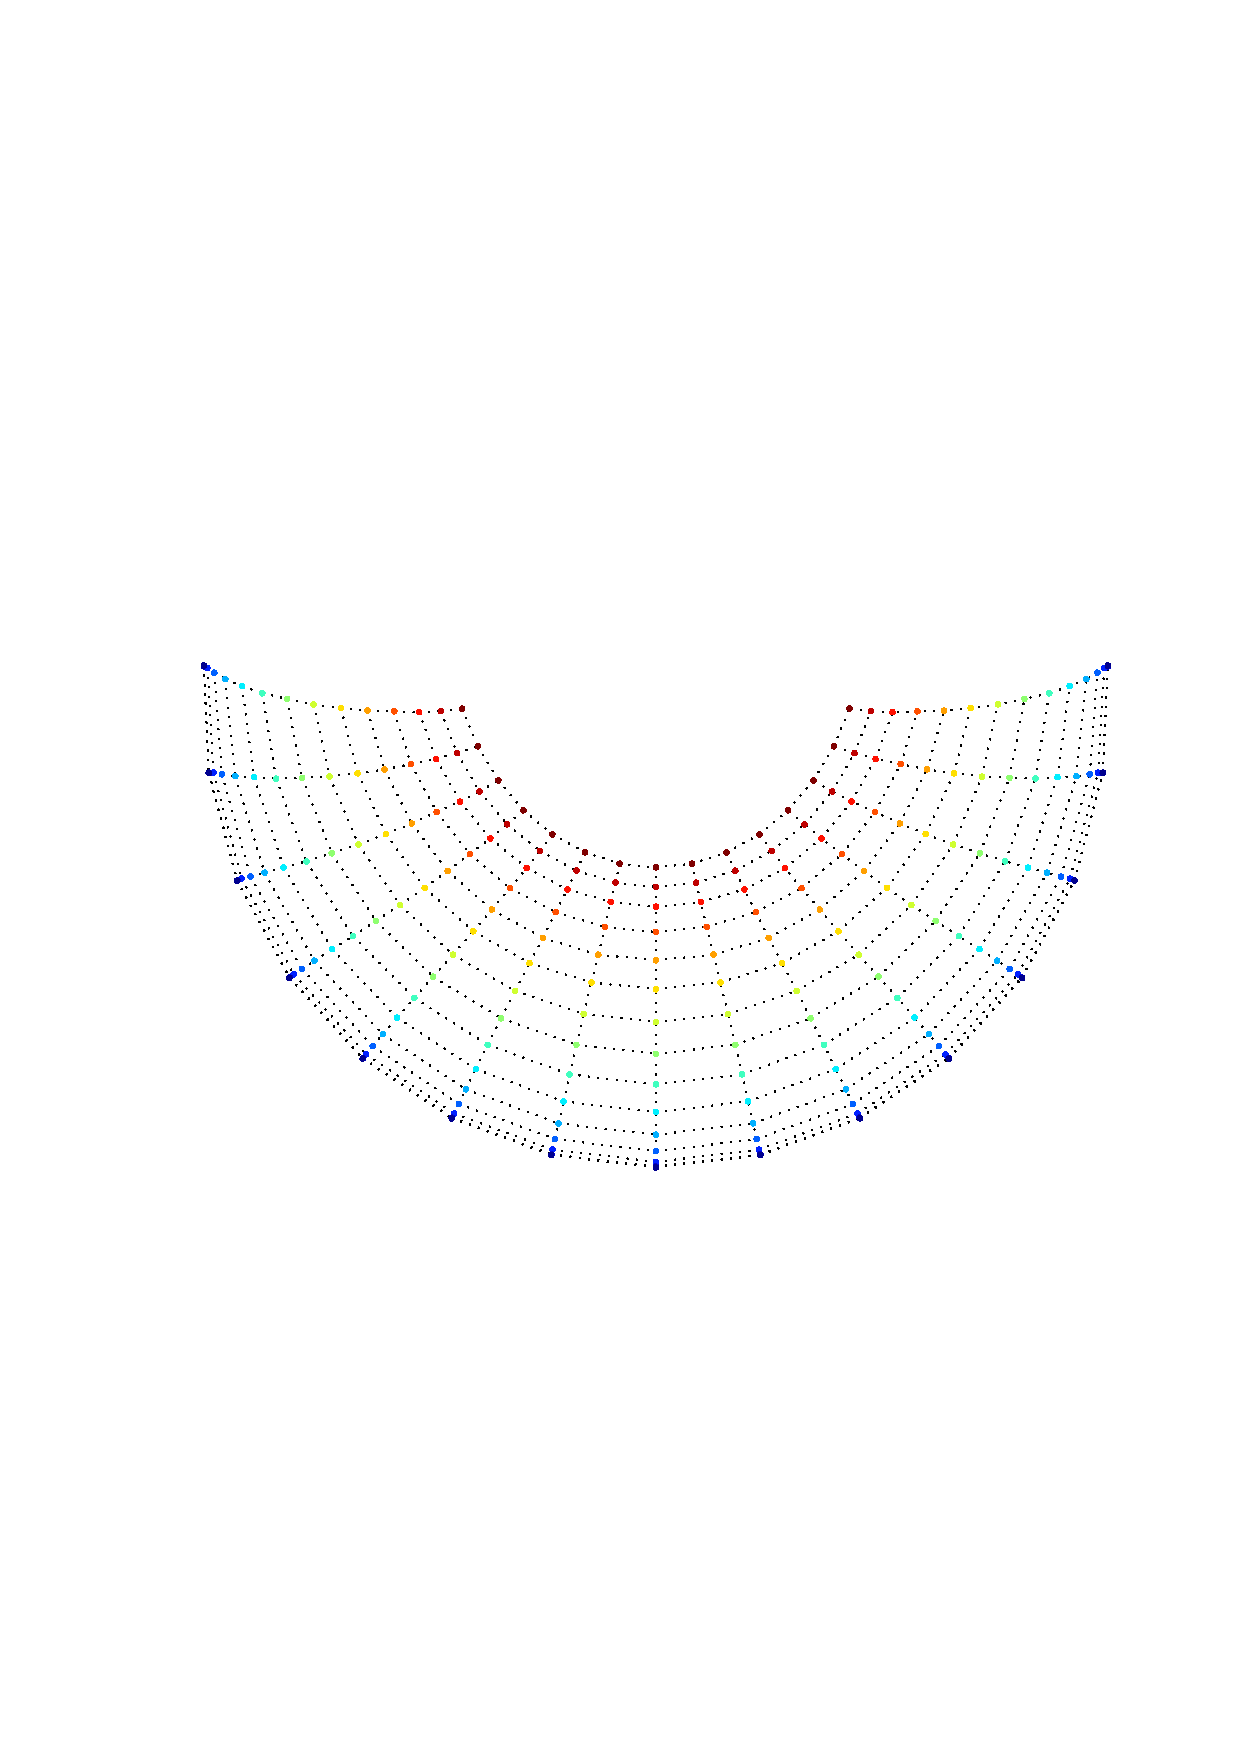
\includegraphics[width = .4\columnwidth]{/Users/fhuszar/Dropbox/thesis/matlab/manifold/figs/Normal_kernel_1.pdf} & $\ell\rightarrow 0$& 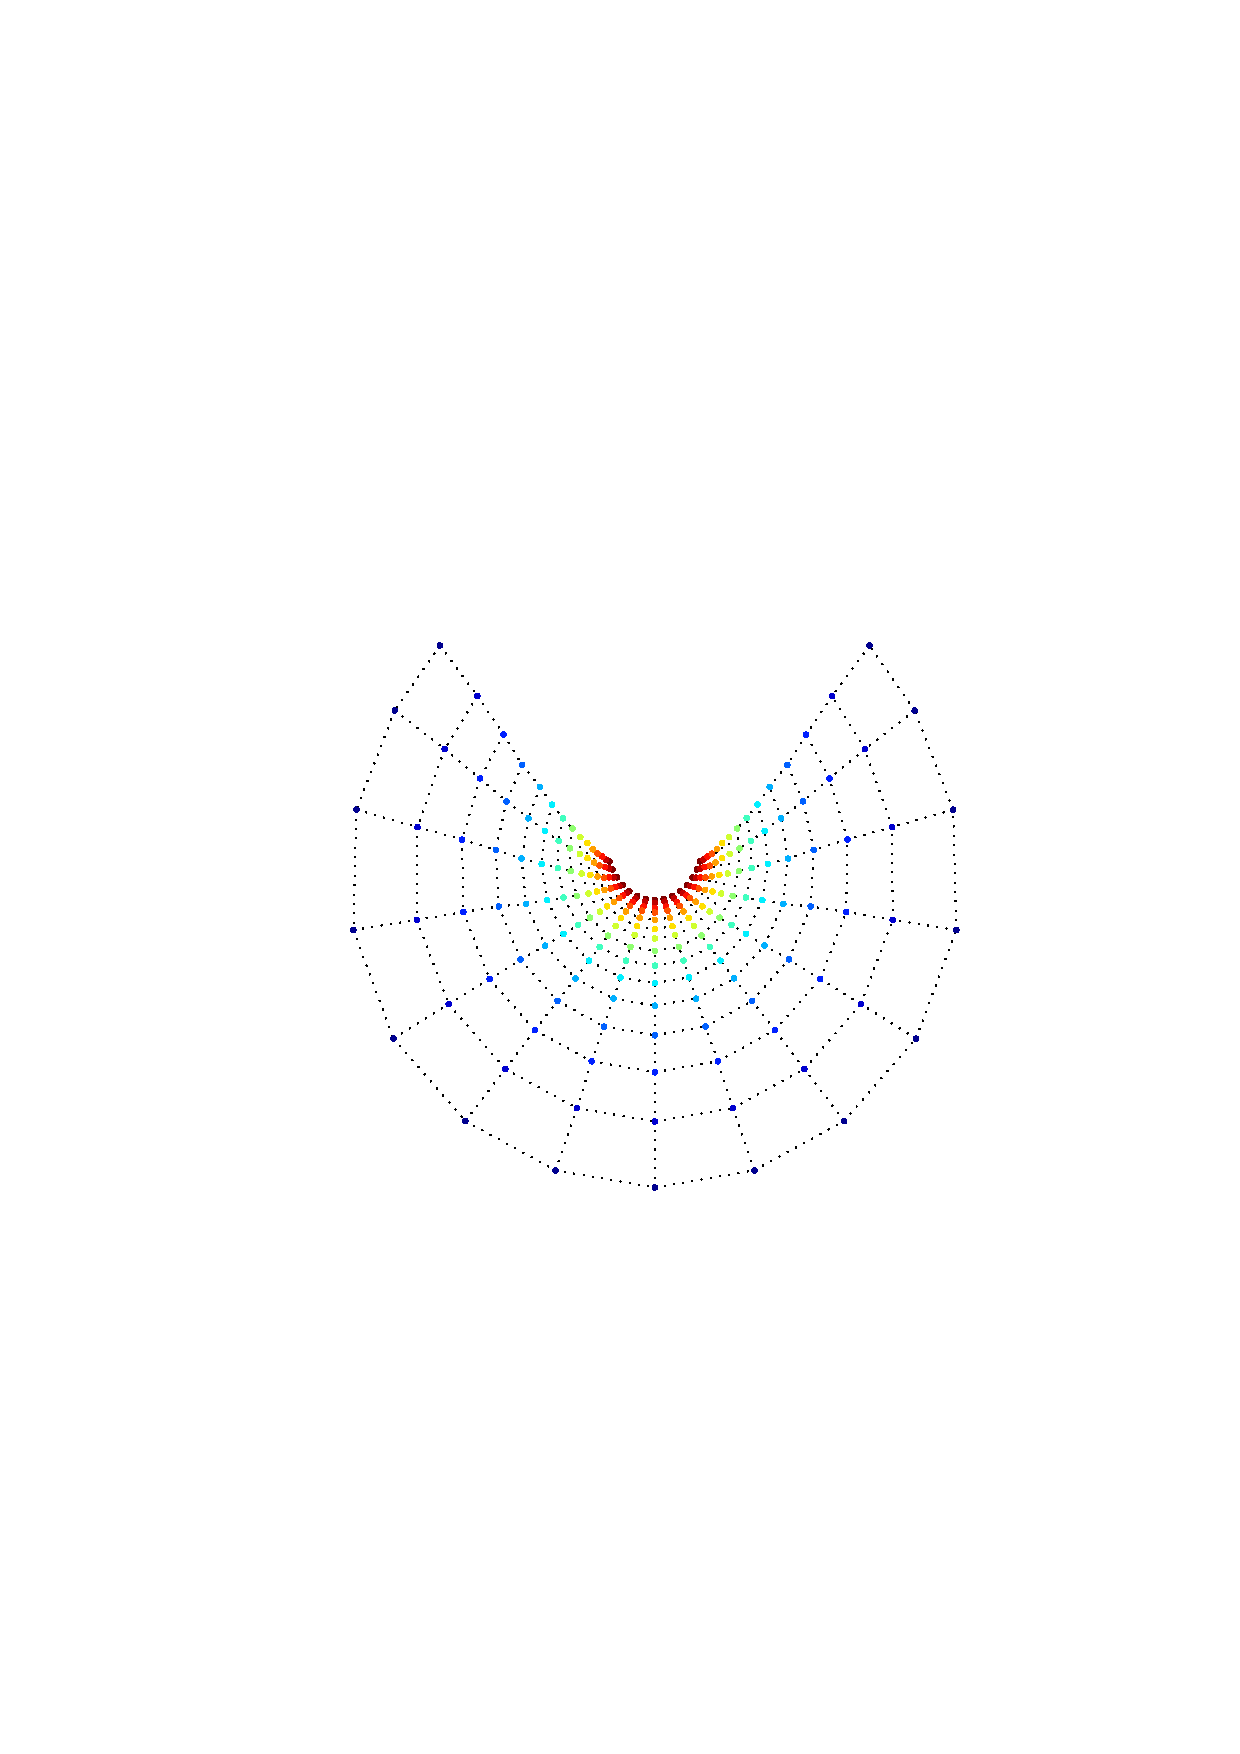
\includegraphics[width = .4\columnwidth]{/Users/fhuszar/Dropbox/thesis/matlab/manifold/figs/Normal_kernel_2.pdf} \\
	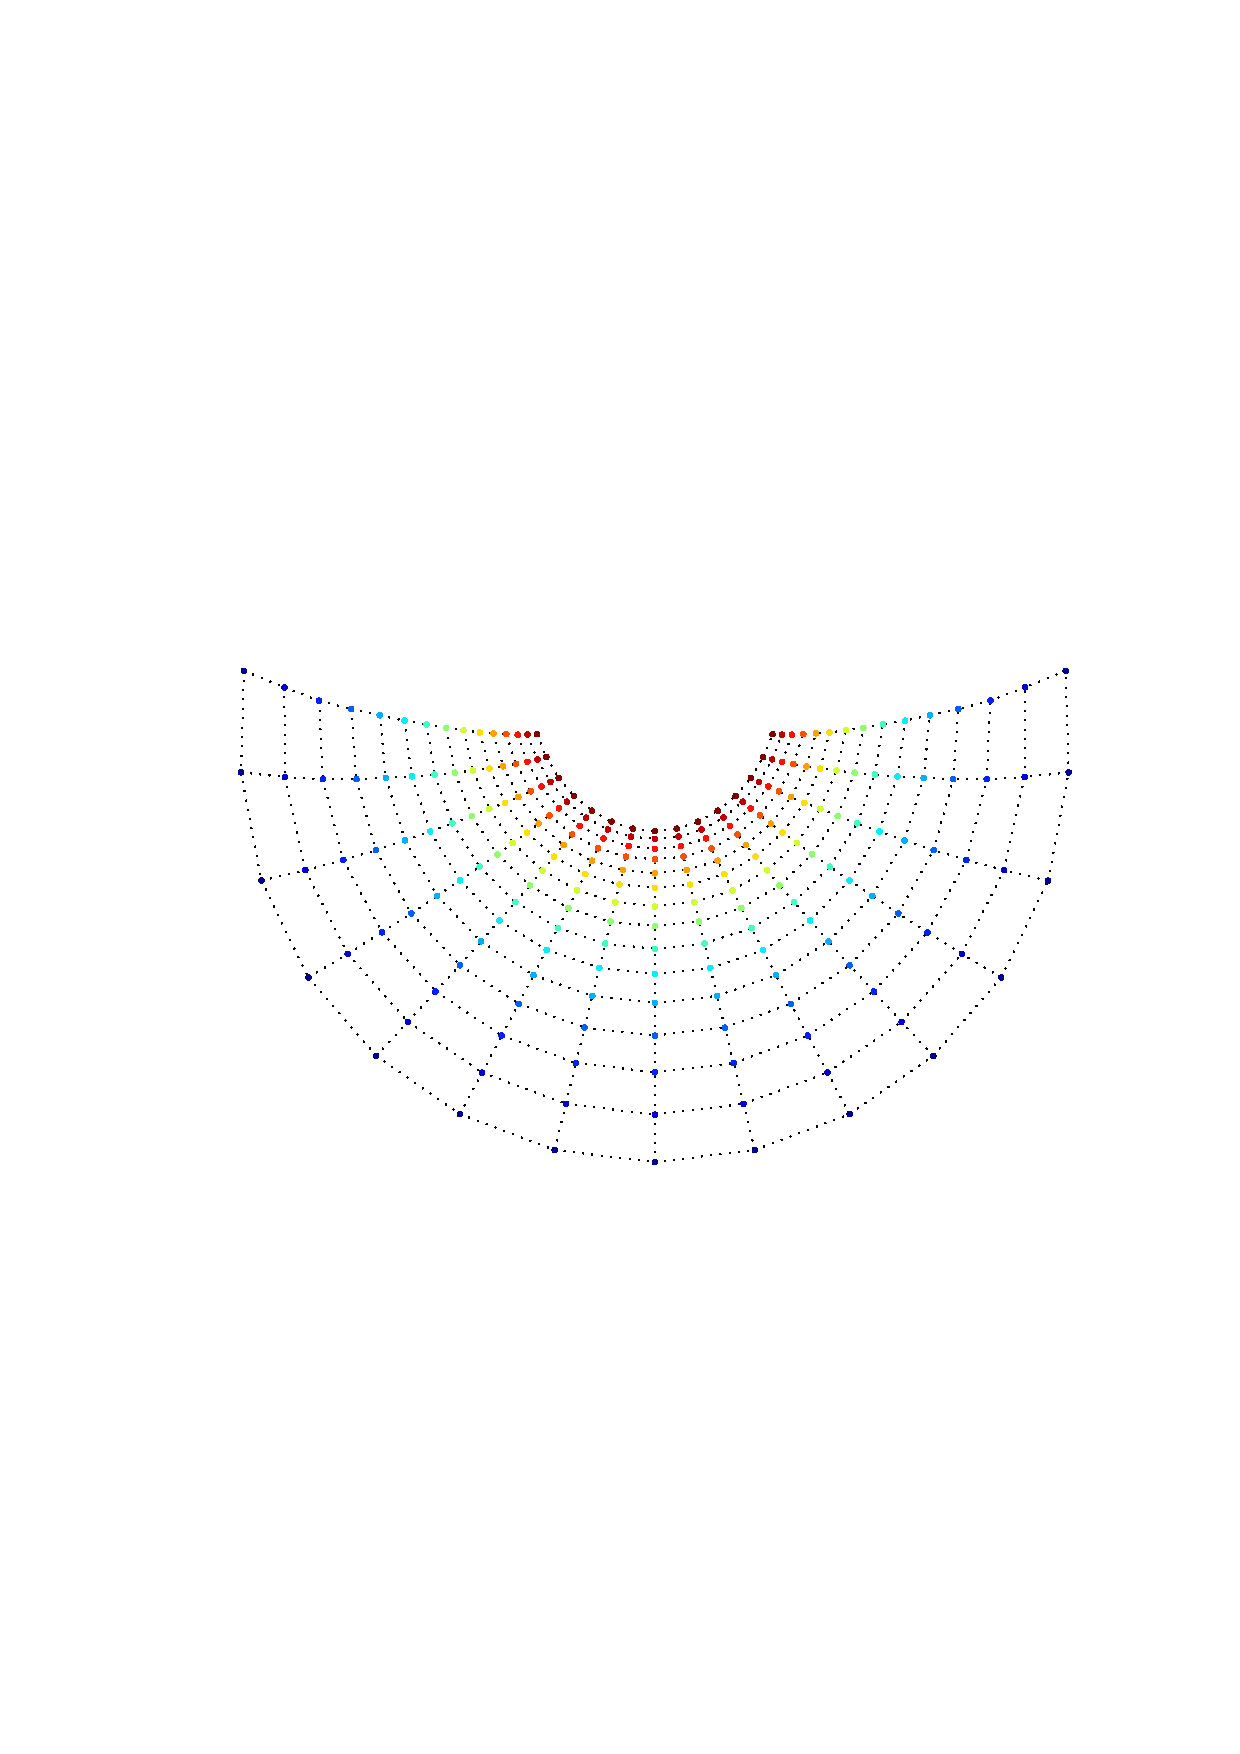
\includegraphics[width = .4\columnwidth]{/Users/fhuszar/Dropbox/thesis/matlab/manifold/figs/Normal_kernel_3.pdf} & $\ell=0.5$ & \includegraphics[width = .4\columnwidth]{/Users/fhuszar/Dropbox/thesis/matlab/manifold/figs/Normal_kernel_4.pdf} \\
	\includegraphics[width = .4\columnwidth]{/Users/fhuszar/Dropbox/thesis/matlab/manifold/figs/Normal_kernel_5.pdf} & $\ell=2$ &  \includegraphics[width = .4\columnwidth]{/Users/fhuszar/Dropbox/thesis/matlab/manifold/figs/Normal_kernel_6.pdf} \\
	\includegraphics[width = .4\columnwidth]{/Users/fhuszar/Dropbox/thesis/matlab/manifold/figs/Normal_kernel_7.pdf} & $\ell=5$ &  \includegraphics[width = .4\columnwidth]{/Users/fhuszar/Dropbox/thesis/matlab/manifold/figs/Normal_kernel_8.pdf} \\
	\end{tabular}
	\end{center}
	\caption{Maps of the statistical manifold induced by the (quadratic) kernel score and the spherical kernel score over Gaussian distributions for different setting of the kernel bandwidth parameter. The two panels in the top row $\ell\rightarrow 0$ correspond to the limiting cases of the Brier score and the spherical score. It can be seen that as the bandwidth increases, both scores shift their sensitivity to distributions with higher variance (red). For equal bandwidth, the spherical kernel score is more sensitive to distributions with larger standard deviation.}
\end{figure}

The main purpose of this section is to visualise differences between the geometries induced by various divergence measures over the same set of distributions. A particularly interesting divergence that we will use in subsequent chapters is that induced by the (quadratic) kernel scoring rule from (section \ref{sec:kernel_scoring}). The kernel scoring rule itself is very flexible, and its properties are dictated by the choice of kernel function.

For several well-known kernels the divergence between univariate Gaussians can be computed in closed form.\citep{tailoring_density} For the squared exponential kernel $k_{\ell}(x,x')=\nicefrac{1}{\ell}\exp(-\frac{(x-x')^2}{\ell^2})$ the divergence is given by the following formula:

\begin{equation}
	\divergence{k_{\ell}}{\Normal_{\mu_1,\sigma_1}}{\Normal_{\mu_2,\sigma_2}} = \frac{1}{\sqrt{\ell^2+2\sigma_1^2}} + \frac{1}{\sqrt{\ell^2+2\sigma_2^2}} - \frac{2}{\sqrt{\ell^2+\sigma_1^2 + \sigma_2^2}}\exp\left(-\frac{(\mu_1 - \mu_2)^2}{2(\ell^2 + \sigma_1^2 + \sigma_2^2)}\right)
\end{equation}

The above formula can be derived from the following general expression for the inner product between mean embeddings:

\begin{align}
	\scalar{\mu_{\Normal(\mu_1,\sigma_1)}}{\mu_{\Normal(\mu_2,\sigma_2)}}_{k_{\ell}} &= \expect{x\sim \Normal(\mu_1,\sigma_1)}\expect{x' \sim \Normal(\mu_1,\sigma_1)} k_{\ell}(x,x')\\
	&= \frac{1}{\sqrt{\ell^2 + \sigma_1^2 + \sigma_2^2}}\exp\left(-\frac{(\mu_1 - \mu_2)^2}{2(\ell^2 + \sigma_1^2 + \sigma_2^2)}\right)
\end{align} 

The first fact one may observe is that unlike the KL divergence, the kernel divergence is bounded from above by $\nicefrac{2}{\ell}$. This upper bound is approached when computing divergence between two infinitesimally narrow Gaussians $\sigma_1,\sigma_2\approx 0$ that are far apart $\vert \mu_1 - \mu_2 \vert > 0$. The divergence is also bounded from below by $0$ and it is $0$ exactly when the two distributions are identical, confirming that this kernel function gives rise to a strictly proper scoring rule.

The Brier score is a special case of this divergence as the lengthscale of the kernel $\ell$ decreases to $0$. In that case we obtain the following expression:

\begin{equation}
	\divergence{Brier}{\Normal_{\mu_1,\sigma_1}}{\Normal_{\mu_2,\sigma_2}} = \frac{1}{\sqrt{2\sigma_1^2}} + \frac{1}{\sqrt{2\sigma_2^2}} - \frac{2}{\sqrt{\sigma_1^2 + \sigma_2^2}}\exp\left(-\frac{(\mu_1 - \mu_2)^2}{2(\sigma_1^2 + \sigma_2^2)}\right)
\end{equation}

We can immediately see that unlike the kernel score with a positive lengthscale, the Brier score is not bounded from above. It diverges for very small values of the variances $\sigma_1$ and $\sigma_2$. It is still non-negative and strictly proper.

To illustrate the differences between the various divergences between Gaussian distributions, we first applied the ISOMAP embedding technique to the one-dimensional manifold of zero-mean Gaussians, whose sole free parameter is the standard deviation. I chose a logarithmically spaced grid of standard deviation values, then used the ISOMAP algorithm to embed the distributions on the real line. The logarithmic spacing is useful as the KL divergence now depends only on the difference in the logarithm of variances, therefore when these distributions are embedded according to the KL divergence, we expect to get a uniform, linearly spaced grid.

Figure \ref{fig:fig:Normal_varonly_comparison} compares the statistical manifold induced by the KL and Brier divergences, as well as by the kernel divergence with different choices of the kernel bandwidth parameter $\ell$. As expected, when the KL divergence is used the numerical algorithm spreads the distributions uniformly on the real line. We can see that compared to the KL divergence, the Brier divergence is more sensitive to differences between narrow distributions, whose standard deviation is small. In case of the kernel score, with increasing kernel brandwith the focus shifts from narrow distributions towards distributions with larger variance. In the range mapped in this figure ($0.05 \leq \sigma \leq 1$) the kernel bandwidth $\ell=0.1$ mimics the behaviour of the KL divergence the best.

For these distributions the KL divergence is scale-free: the divergence between two zero-mean Gaussians with variance $\sigma_1=0.05$ and $\sigma_2 = 0.1$ is the same as the divergence between $\sigma_1=0.5$ and $\sigma_2 = 1$. The kernel score on the other hand has a characteristic brandwith, and is therefore not scale free: when the brandwith is chosen to be $\ell=1$, the largest shown in Figure $\ref{fig:Normals_kernel_comparison}$, the distance between $\sigma_1=0.05$ and $\sigma_2 = 0.1$ is only about one tenth of the distance between $\sigma_1=0.5$ and $\sigma_2 = 1$.

In Figure \ref{fig:Normals_varonly_magnification} I plotted the local distances on the various manifolds relative to distances induced by the logarithmic score. Higher values on the plot indicate a region where local distances are magnified in comparison to the KL divergence, which can be interpreted as a region in which the particular scoring rule is more sensitive to small differences. Observe how changing the kernel bandwidth shifts the most sensitive region of the kernel scoring rule.

These figures highlight how the choice of the kernel allows us to fine-tune properties of the divergences and the corresponding manifold. We can use this flexibility to tailor the divergence to our application \citep{tailoring}. However, as discussed in chapter \ref{sec:scoring_rules} this flexibility also poses a challenge in applications where there is no principled way of choosing kernel hyperparameters.

\subsection{Gamma distributions}

We can look at the geometry Shannon's entropy induces within another two-parameter family of continuous distributions, Gamma distributions. Gamma distributions are strictly positive, their probability density function of Gamma distributions is as follows:

\begin{equation}
(x) = \beta^{\alpha}\frac{1}{\Gamma(\alpha)} x^{\alpha-1} \exp(-\beta x)
\end{equation}

where $\alpha,\beta > 0$ are called shape and rate parameters respectively. Special cases of Gamma distributions are exponential distributions when $\alpha=1$.

The KL divergence between Gamma distributions can be computed in closed form and is given by the following formula:

\begin{equation}
	\KL{\Gamma_{\alpha_1,\beta_1}}{\Gamma_{\alpha_2,\beta_2}} = \left(\alpha_1 - \alpha_2\right)\psi\left(\alpha_1\right) - \log\frac{\Gamma(\alpha_1)}{\Gamma(\alpha_2)} + \alpha_1\log\frac{\beta_1}{\beta_2} + \alpha_1\frac{\beta_2 - \beta_1}{\beta_1} \label{eqn:KL_Gamma}
\end{equation}

\begin{figure} % Gamma distribution - Shannon information statistical manifold
	\begin{center}
	\includegraphics{/Users/fhuszar/Dropbox/thesis/matlab/manifold/figs/Gamma_meanvar.pdf}
	\end{center}
	\caption{Map of Gamma distributions on the statistical manifold induced by the logarithmic score and KL divergence. To be comparable to the manifold of Normal distributions in Figure \ref{fig:Normal_meanvar}, the distributions are parametrised by their mean and standard deviation. Distributions are chosen from a uniform grid in this non-standard parameter-space, with their mean ranging between $1$ and $2$, and standard deviation between $0.1$ and $1$. For large values of variance \emph{(yellow and red)} the manifold is asymmetric and dissimilar to that of Normal distributions. However, as variance decreases \emph{(blue)}, by the central limit theorem Gamma distributions approach Gaussians of the same mean and variance, thus the manifold conforms to the fan-like shape that is characteristic of Gaussian distributions.}
\end{figure}

Figure \ref{fig:Gamma_embedding} shows the manifold of Gamma distributions for parameters $a \leq \alpha \leq b, c\leq \beta \leq d$. As we can see this manifold is less symmetric than that of the Gaussians.

For large values of $\alpha$ the standard deviation of the distribution shrinks, and by the central limit theorem, the distribution converges to a Gaussian. We can illustrate this convergence in the manifold structure. For this we first reparametrise the Gamma distribution in terms of its mean and standard deviation. The mean and standard deviation of a Gamma distribution with parameters $\alpha$ and $\beta$ are given by the following formulae:

\begin{align}
	\mu &= \frac{\alpha}{\beta}\\
	\sigma^2 &= \frac{\alpha}{\beta^2}
\end{align}

Solving for $\alpha$ and $\beta$ in these equations we get

\begin{align}
	\alpha &= \frac{\mu^2}{\sigma^2}\\
	\beta &= \frac{\mu}{\sigma^2}
\end{align}

Plugging these into Eqn.\ \eqref{eqn:KL_Gamma} we can now map Gamma distributions with particular mean and variance. Figure 1 compares Normal and Gamma distributions with mean $\mu\in[0.5,1.5]$ and standard deviation $\sigma\in[0.1,1]$. We can observe that as the variance increases, the manifold of Gamma distributions shows a fan-like structure very similarly that of Normal distributions. However, for larger variance, the distributions look less Gaussian, and the manifold becomes more asymmetric. The effect of the central limit theorem would perhaps be even more prominent for smaller values of $\sigma$, but for those cases that case Eqn.\ \eqref{eqn:KL_Gamma} becomes numerically imprecise, as it relies on look-up-table implementation of the Gamma ($\Gamma$) and bigamma ($\psi$) functions.

% \subsection{Reactor example}

% Not all scoring rules give rise to smooth manifolds. As an extreme example, consider the following decision problem:

% You are uncertain about the temperature of the reactor in a power plant. If the temperature is too high, above a critical temperature $T_{crit}$, the reactor may melt down causing you a loss of \$10 billion. You may choose to shut down the reactor, which costs you \$1 million of lost revenue, irrespective of whether the reactor was indeed overheated or not. You make a probabilistic forecast about the reactor's temperature, and want to make a decision based on that.

% This decision rule segments probabilistic forecasts into only two subsets: those which would result in a ``shut down'' decision, and those that result in a ``keep on going''. 

% \begin{equation}
%   \divergence{reactor}{p}{q} = \left\{
%   \begin{array}{cc} 
%       \begin{array}{cc}
%         0        & p(\{t\geq T_{crit}\}) \geq \ell \mbox{ and } q(\{t\geq T_{crit}\}) \geq \ell\\
%         \ell_1 & p(\{t\geq T_{crit}\})  \geq \ell \mbox{ and } q(\{t\geq T_{crit}\}) \leq \ell\\
%         \ell_2 & p(\{t\geq T_{crit}\})  \leq \ell \mbox{ and } q(\{t\geq T_{crit}\}) \geq \ell
%       \end{array}
%   \end{array}
%   \right.
% \end{equation}

% This divergence therefore does not give rise to a smooth manifold. Figure \ref{fig two_points} shows a map of Gaussian distributions with respect to the KL divergence. The way $\divergence{reactor}{\cdot}{\cdot}$ segments distributions into ``shut down'' or ``keep on going'' types is also shown. We can make the KL divergence more sensitive to the decision problem at hand by considering a convex combination between $\KL{\cdot}{\cdot}$ and $\divergence{reactor}{\cdot}{\cdot}$.



% \chapter{Scoring rules for processes\label{sec:scoring_processes}}
% %!TEX root = ../main.tex
The scoring rule framework presented in chapter \ref{sec:scoring_rules} is already quite general and accommodates a large number of traditional and more modern estimation and scoring techniques. However, there are certain limitations as to what the framework can describe. In this chapter I extend the scoring rule framework further and consider scoring rules for general stochastic processes, in other words, scoring rules in infinite dimensional sampling spaces.

Stochastic processes have enjoyed a surge of interest from the machine learning community thanks to their use in nonparametric Bayesian inference. Nonparametric techniques based on processes like the Gaussian process, Dirichlet process, Indian buffet process have become ubiquitious in modern statistical models. It is interesting to investigate whether and how the scoring rule framework extends to these more general, infinite dimensional statistical models.

To analyse stochastic processes in the scoring rule framework I introduce a novel concept of marginal scoring rules. I show a number of examples of estimation techniques that do not fit the traditional scoring rule framework, but can be accommodated readily in this more general treatment. I will also argue that the notion of strictly proper scoring rules is insufficient when dealing with stochastic processes, and introduce an analogous property I call very strictly proper scoring. 

\section{Extensions of score matching for \iid data}

Let us recall the definition of a strictly proper scoring rule: A score $\score(x,P)$ is called strictly proper if for any two distributions $P,Q$ the following holds:

\begin{equation}
	\expect{x\sim P}S(x,P) \leq \expect{x\sim P}S(x,Q),
\end{equation}
with equality only when $P=Q$.

In this definition we are concerned with the scoring rule's behaviour in expectation under the distribution $P$. In empirical terms taking an expectation is analogous to studying the limit of the empirical mean, as we observe multiple independent copies of the distribution $x$ sampled from $P$.

Indeed, the strictly proper property of a scoring rule under suitable regularity conditions ensures that as we observe infinitely many independent and identically distributed (\iid) samples from a parametric distribution $P_{X\vert\theta}$, the parameter of the distribution can be consistently identified:

\begin{definition}[Score matching estimate]
Let $\{P_{X\vert\theta, \theta\in\Theta}\}$ be a parametric family of distributions and $\score$ a strictly proper scoring rule with respect to this class. The following estimator is called the score matching estimate:
\begin{equation}
	\hat{\theta}_N(x_1,\ldots,x_N) = \argmin_{\theta\in\Theta} \sum_{n=1}^{N}\score(x_n,P_{X\vert\theta}) \label{eqn:score_matching}
\end{equation}
The above equation is an unbiased estimating equation, and under suitable regularity conditions $\hat{\theta}_N(x_1,\ldots,x_N)$ is a consistent estimator, that is if $x_1,\ldots\sim P_{X\vert\theta_0}$\iid
\begin{equation}
	\lim_{N \rightarrow \infty} \hat{\theta}_N(x_1,\ldots,x_N) = \theta_0\hspace{1cm} P_{X\vert\theta_0}\mbox{-\,almost surely}
\end{equation}
\end{definition}

Score matching has been used to fit parametric models for decades. Maximum likelihood estimation is a typical example when the scoring rule is chosen to be the logarithmic score. In more modern work like \citep{kernelmomentmatching}, the kernel scoring rule is used to fit parametric distributions; the technique is referred to as kernel moment matching. Score matcing with the Brier and spherical scores has also been used in meteorology and epidemiology.

The score matching procedure assumes that one observes a sequence of \iid observations repeatedly sampled from the same distribution $P$. However, observed data is not always \iid. Often we want to score non-\iid sequences or sets of variables, and we would still like our parameter estimates to be consistent in some sense. Examples of such non-\iid estimation scenarios include:
\begin{enumerate}
	\item Parameter estimation in non-parametric process models, such as in Gaussian process regression, studying the limit as the size of the training data grows
	\item parameter estimation of a large Markov random field, studying constitency as the image size grows
	\item Parameter estimation in phylogenetic tree models, studying behaviour as the number of species and the size of the tree grows
	\item Bayesian model selection in hierarchical Bayesian models, where instead of \iid assumption we often find exchangeability assumptions
\end{enumerate}

In all of the examples above, we never observe a growing number of independent copies of the same random variable. Instead, we observe higher and higher dimensional marginals of the same single trajectory sampled randomly from a random process. We sample one infinitely large object from a random process once, and we study the behaviour as larger and larger parts of this object are revealed.

The above cases do not readily fit into the scoring rule framework which is specifically concerned with \iid observations from the same, fixed dimensional distribution. To analyse these cases we can extend the scoring rule framework so that we allow scoring of partial observations. Let us consider the following definition of marginal scoring rules:

\begin{definition}[Marginal scoring rule]
Let $\Xe$ be a countably infinite index set, $I\subseteq\Xe$ a subset of indices. A marginal scoring rule $R_I$ over this index set is a function that assigns a real value, $R_{I}(y_{I},\Pi)$,  to a process measure $\Pi\in\probmeasures{\Ye^{\Xe}}$ and an observed marginal $y_{I}\in\Ye^{I}$.
\end{definition}

Marginal scoring rules allow one to calculate the score of a forecast on the basis of a partial observation $y_{I}$. For example, if $\Pi$ is a distribution over images, a marginal scoring rule can assign a score to $\Pi$ even if we only observe the right-hand corner of the image, and the rest remains hidden. This definition therefore allows us to study what happens as higher and higher dimensional marginals are revealed, as we desired.

Observe, that the traditional \iid scoring rule framework can be expressed in terms of marginal scoring rules over \iid processes. Instead of thinking about repeatedly sampling from a finite dimensional distribution, we can imagine sampling one infinitely long sequence first, but then revealing longer and longer sub-sequences from it. Let $\Xe$ be the set of natural numbers, and $\Pi$ an \iid process such that $\Pi_{I}(y_{I}) = \prod_{i\in I} P(y_i)$, then we can construct marginal scoring rules as follows:

\begin{equation}
R_{I}(y_{I},\Pi) = \frac{1}{\vert I \vert} \sum_{i\in I_n} S(y_i,P)\label{eqn:decompose},
\end{equation}
where $S$ is a strictly proper scoring rule over $\Ye$.

The marginal scoring rules in eqn. \eqref{eqn:decompose} are useful in the following sense.

\begin{statement}[Consistency of marginal scoring for \iid processes]
Let us take a monotonically increasing sequence of index sets $I_1\subseteq\ldots\subseteq I_N \subseteq \ldots \subseteq \Xe$, such that $\cup_{N=1}^{\infty} I_N = \Xe$ and $\score(y,P)$ be a strictly proper scoring rule over $\Ye$ with respect to the class of marginals $P_{\theta}$. Let $\Pi_{\theta}$ denote the \iid process over $\Ye^{\Xe}$ with marginal $P_{\theta}$. Then ``typically'' the following limit holds

\begin{align}
\argmin_{\theta}R_{I_n}(y_{I_n},\Pi_{\theta^{*}}) =  \argmin_{\theta} \frac{1}{\vert I_N \vert} \sum_{i\in I_N} \score(y_i,P_{\theta}) \stackrel[N\rightarrow\infty]{P_{\theta^{*}}}{\longrightarrow} \theta^{*}
\end{align}
\end{statement}

The above equation is the same as score matching, but now we look at it slightly differently. Intuitively, consistency in this general sense means that as larger and larger marginals of a trajectory drawn from the process $\Pi_{\theta}$ are revealed, the scoring rule can identify the true parameter $\theta$ of the process from which the trajectory was drawn. When a general family of marginal scoring rules has this property, we will call it the very strictly proper property:

\begin{definition}[Very strictly proper marginal scoring]\label{thm:very_strictly_proper}
Let $R_{I}$ be a family of marginal scoring rules over processes on $\Ye^{\Xe}$, $\Qe = \{\Pi_\theta, \theta\in\Theta\}$ a family of process measures over $\Ye^{\Xe}$. $R_{I}$ is very strictly proper with respect to $\Qe$ if for any monotonically increasing sequence of index sets $I_1\subseteq\ldots\subseteq I_N \subseteq \ldots \subseteq \Xe$, such that $\cup_{N=1}^{\infty} I_N = \Xe$ the following limit holds:
\begin{align}
\lim_{N\rightarrow\infty} \argmin_{\theta} R_{I_N}(y_{I_N},\Pi_{\theta}) = \theta^{*}\hspace{1cm}\Pi_{\theta^{*}}\mbox{\,almost surely}
\end{align}
\end{definition}

In the following sections I show families of marginal scoring rules $R_I$, that do not simply decompose into sums of scoring rules on $\Ye$ for marginals $\Pi$, but most of which still have the very strictly proper property.

\subsection{Maximum product of spacings score}

The first example, \emph{maximum product of spacings (MPS) estimation} is not normally considered in the context of scoring rules, but we can now interpret it as part of this general framework of marginal scoring rules. It is an estimation technique based on the observation that if a set of points are sampled from a one dimensional uniform distribution, then the spacing between neighbouring samples should be roughly the same. Thus, a viable ``scoring rule'' for the uniform distribution measures how uneven the spacing between neighbouring samples are. The evenness of a set of numbers can be measured by the difference between arithmetic and geometric means. The above argument can be extended to arbitrary real probability distributions by noting that transforming a general non-uniform random variable by its cumulative distribution function results in a uniform random variable between $0$ and $1$.

\begin{definition}[Product of spacings score]
	Let $y_1,\ldots,y_N$ independent random variables on the real line $\Reals$. Let $P$ be a distribution over $\Reals$ with cumulative distribution function $F_{P}$. Let $\pi:\{1,\ldots,N\}\mapsto\{1,\ldots,N\}$ a rank ordering such that $n<m \implies y_{\pi_{n}}\leq y_{\pi_{m}}$. For convenience of notation let us further define $y_{\pi_0}\defeq 0$ and $y_{\pi_{N+1}}\defeq 1$.
	\begin{equation}
		R^{PS}_N(y_1,\ldots,y_N,P) = - \frac{1}{N+1} \sum_{n=0}^{N} \log \left(F_P\left(y_{\pi_{n+1}}\right) - F_P\left(y_{\pi_{n}}\right) \right)
	\end{equation}
\end{definition}

It is shown in \citep{http://fir.nes.ru/tildegkosenok/MPS.pdf} that subject to smoothness assumptions, MPS estimation, which minimises $R^{PS}_N$ is consistent when $y_n$ are sampled \iid from a distribution. That is
\begin{align}
\argmin_{\theta}R^{PS}_{N}(y_1,\ldots,y_N,\Pi_{\theta^{*}}) \stackrel[N\rightarrow\infty]{P_{\theta^{*}}}{\longrightarrow} \theta^{*}
\end{align}

Furthermore, the estimator is often statistically more efficient than maximum likelihood estimation (MLE) \citep{http://fir.nes.ru/tildegkosenok/MPS.pdf}. The drawback of the product of spacings score is that it does not readily generalise to multivariate distributions, and it requires the knowledge of the cumulative distribution function to be calculated.

\subsection{Decision theoretic scoring and $F_{\beta}$ scores}

Further examples of scores that do not decompose as in \eqref{eqn:decompose} can be constructed on decision theoretic grounds when the action and the loss that we minimise itself depends on multiple outcomes. For example in a binary case we may want to penalise imbalanced forecasters, so we prefer forecasters that produce about as many false positives as false negatives while at the same time minimise the total number of false predictions.

Most of these complicated objectives can be achieved by optimising something like the $F_{\beta}$ score, which is applied in a variety of statistical applications \citep{}:

\begin{equation}
	F_\beta = (1-\beta^2)\frac{\mbox{precision}\cdot\mbox{recall}}{\beta^2 \mbox{precision} + \mbox{recall}}
\end{equation}

The $F$ score depends on a whole sample and cannot be decomposed as a sum of terms that score each sample independently. Hence it is a good example of general marginal scoring rules.

\section{Non-\iid processes}

In the examples I gave above, the scoring rule did not decompose into a sum of univariate scores as in \eqref{eqn:decompose}, but we would still use these scores to score and estimate \iid processes. The present framework also accommodates more general cases when we want to score non-\iid processes, such as hierarchical Bayesian models, Markov random fields, processes over tree structures or Gaussian processes.

The simplest and most widely adopted scoring rule of this form is log-score (assuming marginals of $\Pi$ have densities $P_{I_n}$), which is also called (negative) evidence:

\begin{align}
	R_{I_N}(x_{I_N},\Pi) = - \frac{1}{\vert I_N \vert}\log P_{I_n}(y_{I_n}),
\end{align}

\subsection{Bayesian model selection}

The consistency of the maximum likelihood estimator has been studied with respect to particular classes of models and processes. A particularly interesting case is when the process $\Pi$ is exchangeable.

By De Finetti's theorem, exchangeable sequences of random variables have a representation as mixtures of \iid sequences, and can therefore be interpreted as hierarchical Bayesian models. Let's say we have a model $\model$, under which $y_n$ are conditionally \iid given some parameters $\theta$. Given some observed data y, the model's evidence is given by the following formula:

\begin{align}
	\mbox{evidence}(\model) &= R_{log}(y_{1:N},\Pi_{Y\vert\model})\\
		&= \log P_{Y_{1:N}\vert\model}(y_{1:N})\\
		&= \log \int \prod_{n=1}^{N} P_{Y_1\vert\theta}(y_n) P_{\theta\vert\model}(\theta) d\theta
\end{align}

We can observe that even though conditioned on $\theta$ subsequent $y_n$ variables are independent, marginally they are dependent, therefore the evidence does not decompose into a sum of terms per data-point as it would for marginally \iid models.

The evidence is accepted as a very robust criterion for Bayesian model selection and is thought to be particularly robust against over-fitting. On the other hand it is often intractable to compute exactly for complicated models, and one has to rely on various approximations such as the Bayesian information criterion (BIC)\citep{}, Akaike information criterion (AIC)\citep{}, variational lower bounds, or expectation-propagation (EP)\citep{}.

We can generalise Bayesian model selection by replacing the log-score with another family of marginal scoring rulea, such as the quadratic kernel rule from Eqn.\ \eqref{eqn:kernel_scoring}. When we use the kernel scoring rule for Bayesian model selection, it decomposes clearly into two terms, which intuitively represent the trade-off between accuracy and model flexibility.

\begin{align}
	\divergence{k}{\delta_{y}}{\Pi_{Y\vert\model}} &= \Hnorm{k(\cdot,y) - \mu_{Y\vert\model}}^2\\
		&= \Hnorm{k(\cdot,y) - \expect{\theta\sim p_{\theta\vert\model}}\mu_{Y\vert\theta}}^2\\
		&= \expect{\theta\sim p_{\theta\vert\model}} \Hnorm{k(\cdot,y) - \mu_{Y\vert\theta}}^2 - \expect{\theta\sim p_{\theta\vert\model}}\Hnorm{\mu_{X\vert \theta,\model} - \mu_{X\vert\model}}^2\\
		&= \underbrace{\expect{\theta\sim p_{\theta\vert\model}} \divergence{k}{\delta_{y}}{p_{X\vert\theta}} }_{\mbox{average accuracy}} -  \underbrace{\information{k}{X}{\theta}}_{\mbox{diversity}}
\end{align}

After \citep{} one may call this the ambiguity decomposition of the quadratic kernel score. As the Brier score is a special case of the kernel scoring rule, it naturally admits the same decomposition. The decomposition suggests that a good model is
\begin{description}
	\item[accurate:] it forecasts observed data relatively accurately on average for all parameters, and
	\item[diverse:] it is capable of expressing a diverse range of behaviours via its parameters
\end{description}

\subsection{Pseudo-likelihood}

We can also study the pseudo-likelihood score in this context. In machine learning this score may be called the leave-one-out cross-validation error.

\begin{align}
R(y_{I_N},\Pi) = - \frac{1}{\vert I_N \vert} \sum_{n\in{I_N}}\log P_{Y_n\vert Y_{I_n\backslash\{n\}}}(y_n)
\end{align}

We already noted that the pseudo-likelihood score is strictly proper, so under multiple sampling from the same size marginal, pseudo-likelihood it is typically consistent. But we can also study the limit as larger and larger marginals are considered.

The most typical application of pseudo-likelihood estimation is parameter estimation in Markov random fields. A finite graph Markov-random field is a stochastic process, where each variable is conditionally independent of the rest of the trajectory given a finite number of other variables, known as the Markov-blanket of the variable. A common example of a finite graph Markov random field is the two-dimensional square lattice Isling model \citep{Dawid's paper}. This model and its generalisations have found several applications in computer vision and image processing \citep{}.
 
Typically when studying consistency properties of pseudo-likelhiood, authors show that the pseudo-likelihood score is strictly proper and thus pseudo-likelihood estimation is consistent under repeated sampling from a finite dimensional Markov random field. In this chapter we are interested in consistency of estimation from a single draw from an infinite MRF, in the limit as larger and larger sub-graphs are observed. It turns out pseudo-likelihood estimation is consistent in this stricter sense, too \citep{GemanGraffigne}, therefore we can call it a very strictly proper scoring rule.

Pseudo-likelihood estimation can be used in other cases where computing the logarithmic score is intractable, such as estimating phylogenetic trees in models such as the infinite sites model \citep{something, something} . In this application the observed data are a set of related genomes, that are thought to have evolved from a common ancestor genome through a process of random mutations and recombinations and can therefore be related via a phylogenetic tree. The task is to infer the latent phylogenetic tree underlying the data, and to estimate model parameters such as the relative rate of mutation and recombination events.

This estimation problem is hard because of the exponential number of phylogenetic trees consistent with any one dataset. Computing the marginal likelihood (or logarithmic score, as in Eqn.\ \eqref{eqn:marginal_log_score}) is intractable as it involves computing a non-trivial sum over phylogenetic trees. However, computing the conditional distribution of just one gene (or segregating site on the DNA), conditioned on the observed values of other genes can be performed relatively efficiently in certain models, and thus pseudo-likelihood estimation may be efficiently applied to these models. It is an open question whether pseudo-likelihood estimation, or indeed maximum likelihood estimation is consistent in the limit of increasing number of alleles and species.

\subsection{Information quantities for stochastic processes}

Finally, it is a natural question to ask, whether it possible, or if at all useful to define information quantities, such as entropy and divergence, between stochastic processes. Following definition \ref{thm:very_strictly_proper} it makes sense to replace expectations with limits in these definitions.

\begin{definition}[Entropy and divergence for processes]\label{thm:process_entropy_divergence}
Let $R_{I}$ be a family of marginal scoring rules over processes on $\Ye^{\Xe}$, $R_{I}$ is very strictly proper family of marginal scoring rules.Consider a monotonically increasing sequence of index sets $I_1\subseteq\ldots\subseteq I_N \subseteq \ldots \subseteq \Xe$. Let us define the entropy or a random process $\Pi$ as follows

\begin{equation}
	\genentropy{R}{\Pi} = lim_{N\rightarrow\infty}R_{I_N}(X_{I_N},\Pi) \mbox{, where } X \sim \Pi
\end{equation}

Similarly, let us define the divergence between two processes $\Pi$ and $\Xi$ as
\begin{equation}
	\divergence{R}{\Pi}{\Xi} =  lim_{N\rightarrow\infty}R_{I_N}(X_{I_N},\Xi) - R_{I_N}(X_{I_N},\Pi) \mbox{, where } X \sim \Pi
\end{equation}
\end{definition}

In general the quantities defined above are random quantities. When the scoring rule $R$ is the logarithmic score, and $\Pi$ is a stationary stochastic process, the Shannon-McMillan-Breiman theorem ensures that the entropy defined this way converges almost surely to deterministic value \citep{}, called the source entropy of the probabilistic source $\Pi$. Under the same conditions the divergence $\divergence{R}{\Pi}{\Xi}$ also converges and is strictly positive for $\Pi \neq \Xi$.

We can conclude that in certain special cases the entropy and divergence quantities defined in definition \ref{thm:process_entropy_divergence} make sense and are useful, but very likely these generalisations are too general for practical purposes.

\part{Scoring rules and divergences in Bayesian analysis}

\chapter{An introduction to scoring rules}

In this section I describe scoring rules that can be used to assess the performance of probabilistic forecasting models. The scoring rule framework allows us to define useful generalisations of well-known information quantities, such as entropy, mutual information and divergence. Based on this, scoring rules allow for defining rich geometries of probabilistic models, which can be exploited in a variety of statistical applications, such as parameter estimation, approximate inference and optimal experiment design.

Imagine we want to have build a probabilistic forecaster that predicts the value of a random quantity $\X$. We can describe any such probabilistic forecaster as a probability distribution $P(x)$ over the space of possible outcomes $\Xe$. After observing the outcome $X=x$ we want to assess how good our predictions were: \emph{scoring rule} is a general term to describe any function that quantifies this: if the outcome is $X=x$, and our prediction was $P$ we incur a score $\score (x,P)$. Scoring rules, by convention, are interpreted as losses, so lower values are better. A good example of scoring rules is the logarithmic score, or simply the log score: $\score_{\mbox{log}}(x,P) = -\log P(\x)$, which is used in maximum likelihood estimation. It is certainly a very important scoring rule and has several unique features (see section \ref{sec:logscore}), but it is not the only one. I will give further examples of scoring rules in section \ref{}. Mathematically, a scoring rule is any measurable function that maps an outcome-probability distribution pair onto real numbers: $\score:\Xe\times\probmeasures{\Xe}\mapsto\mathcal{R}\cup\{\infty\}$.

\section{Information quantities}

A scoring rule allows us to define the following, useful information quantities \cite[see also][]{Blaetal2332}.

\begin{definition}[Generalised entropy]
Given a scoring rule $\score:\Xe\times\probmeasures{\Xe}\mapsto\Reals$, let us define the generalised entropy of a distribution $P\in\probmeasures{\Xe}$ as follows:
\begin{equation}
	\genentropy{S}{P}= \expect{x\sim P} \score(x,P)
\end{equation}
\end{definition}


This entropy measures how hard it is to forecast the outcome on average, when true distribution $P$ of outcomes is known and used as the forecasting model. We can often think of this quantity as a measure of uncertainty in the distribution, and as we will see this quantity is also closely related to the Bayes-risk of decision problems (section \ref{sec:loss_scoring}).

A further quantity of interest is the divergence between two distributions $P$ and $Q$.

\begin{definition}[Generalised divergence]
Given a scoring rule $\score:\Xe\times\probmeasures{\Xe}\mapsto\Reals$, let us define the divergence between two distributions $P,Q\in\probmeasures{\Xe}$ as follows:
	\begin{equation}
		\divergence{\score}{P}{Q} = \expect{x\sim P} \score(x,Q) - \expect{x\sim P} \score(x,P)\mbox{.}\label{eqn:def_divergence}
	\end{equation}
\end{definition}

\TODO{Mention Bregman divergences \cite{http://bit.ly/Ojhpw4}}.

The divergence measures how much worse we are at forecasting a quantity $\X$ sampled from a distribution $P$ when instead of using the true distribution $P$, we use an alternative probability distribution, $Q$. Ideally, we would like to see that using the true model $P$ should always be better or at least as good as using any alternative model $Q$, but this is not automatically true for all scoring rules. A scoring rule that has this property is called a \emph{proper scoring rule}.

\begin{definition}[Proper scoring rule]
	$\score:\Xe\times\probmeasures{\Xe}\mapsto\Reals$ is a \emph{proper scoring rule} with respect to a class of distributions $\Qe$ if $\forall P,Q\in\Qe$ the following inequality holds:
	\begin{equation}
		\expect{x\sim P} \score(x,Q) \geq \expect{x\sim P} \score(x,P),
	\end{equation}
	or equivalently in terms of the divergence $\divergence{\score}{\cdot}{\cdot}$:
	\begin{equation}
		\divergence{\score}{P}{Q} \geq 0.
	\end{equation}
	
	The scoring rule $s$ is said to be \emph{strictly proper} w.\,r.\,t.\ $\Qe$ if equality holds only when $P=Q$.
\end{definition}

The divergence is a measure of the difference between two distributions $P$ and $Q$. Even if the scoring rule is proper, and therefore $\divergence{s}{P}{Q} \geq 0$ always holds, the divergence is normally non-symmetric, that is $\divergence{\score}{P}{Q} \neq \divergence{\score}{Q}{P}$. Divergences are often used to match or approximate some \emph{true} or \emph{ideal} distribution with something \emph{approximate}, so that the divergence between the truth and the approximation is minimal. As we can measure divergence in both ways, there is a question of which direction of divergence is to be calculated.

Definition \eqref{eqn:def_divergence} suggests that the the first argument, $P$, should take the role of the true distribution, and $Q$ the approximate. \TODO{elaborate on this.}

So far we have only introduced quantities describing a single random variable, and comparing probability distributions over the same variable. We can extend the scoring rule framework to define information quantities that describe the relationship between multiple variables. A particularly useful quantity is the value of information, that measures the dependence between.

\begin{definition}[Generalised value of information]
	Let $X,Y$ be random variables with joint distribution $P\in\probmeasures{\Xe\times\Ye}$. Let $\score:\Xe\times\probmeasures{\Xe}\mapsto\Reals$ be a scoring rule over the variable $X$. We define the value of information in variable $Y$ about variable $X$ with respect to the scoring rule $\score$ as
	\begin{equation}
		\information{S}{X}{Y} =  \expect{x\sim P_{X}}\score(x,P_{X})- \expect{y\sim P_{Y}} \expect{x\sim P_{X\vert Y=y}}\score(x,P_{X\vert Y=y})
	\end{equation}
	Alternatively, we can write information in terms of the generalised entropy or divergence functions
		\begin{align}
			\information{\score}{X}{Y} &=  \genentropy{\score}{P_{X}} - \expect{y \sim P_{Y}} \genentropy{\score}{P_{X\vert Y=y}}\\
				&= \expect{y\sim P_{Y}}\divergence{S}{P_{X}}{P_{X\vert Y=y}}
		\end{align}
\end{definition}

This quantity measures the extent to which observing the value of $Y$ is useful in forecasting variable $X$. Remarkably, this information quantity is non-symmetric. Indeed, the definition only requires a scoring rule over the variable $X$, but none over variable $Y$, so defining the value of information in $Y$ about $X$ does not even imply a definition of the value of information in $X$ about $Y$.

If the scoring rule is proper, the value of information is always non-negative. Furthermore, if the scoring rule is strictly proper, the information is zero, if and only if the two variables are independent.

\begin{theorem}
	Let $\score:\Xe\times\probmeasures{\Xe}\mapsto\Reals$ be a strictly proper scoring rule with respect to probability distributions $\probmeasures{\Xe}$, and $P\in\probmeasures{\Xe\times\Ye}$ the joint probability of variables $X$ and $Y$. Then the two statements are equaivalent:
	\begin{enumerate}
		\item $\information{\score}{X}{Y} = 0$
		\item the variables $X$ and $Y$ are independent
	\end{enumerate}
	\begin{proof}
		If $X$ is independent of $Y$, then $\forall y: P_{X\vert Y=y} = P_{X}$, which implies $\forall y:  \divergence{S}{P_{X}}{P_{X\vert Y=y}}=0$, and hence $\information{\score}{X}{Y} = 0$.
		
		On the other hand, $\information{\score}{X}{Y} > 0$ implies $\exists y: \divergence{S}{P_{X}}{P_{X\vert Y=y}} > 0$, therefore by strict propriety of $\score$, $\exists y: P_X \neq P_{X\vert Y=y}$, which contradicts independence.
	\end{proof}
\end{theorem}

As a corollary, strictly proper scoring rules are equivalently strong in the sense that if one detects dependence between variables, than any of them will:

\begin{corollary}
	Let $\score_1,\score_2:\Xe\times\probmeasures{\Xe}\mapsto\Reals$ be two strictly proper scoring rules over $X$. $X$ and $Y$ are two random variables. Then $\information{\score_1}{X}{Y} > 0$ if and only if $\information{\score_2}{X}{Y} > 0$.
\end{corollary}

It also follows that the value of information defined by strictly proper scoring rules is weakly symmetric in the following sense:

\begin{corollary}
	Let $\score_X:\Xe\times\probmeasures{\Xe}\mapsto\Reals$ be two strictly proper scoring rule over $X$ and $\score_Y:\Ye\times\probmeasures{\Ye}\mapsto\Reals$ be two strictly proper scoring rule over $Y$.  Then $\information{\score_X}{X}{Y} > 0$ if and only if $\information{\score_Y}{Y}{X} > 0$.
\end{corollary}

\section{Examples of scoring rules}

After having discussed general properties of scoring rules and information quantities based on them, let us look at particular examples of scoring rule and the entropies and divergences they define.

\subsection{The log score}

The most straightforward, and most widely used scoring rule is the log-score:

\begin{equation}
	\score_{log}(x,p) = - \log p(x) 
\end{equation}

Maximum likelihood estimation can be interpreted as score-matching with the log score:

\begin{equation}
	\theta_{ML} = \argmax_{\theta} \sum_{n=1}^{N} \log p(x_i \vert \theta)
\end{equation}

The associated entropy function is Shannon's differential entropy for continuous distributions

\begin{equation}
	\genentropy{log}{p} = - \int p(x) \log p(x) dx
\end{equation}

The resulting divergence function is the Kullback-Leibler (KL) divergence, which is very widely used in approximate Bayesian inference:

\begin{equation}
	\KL{p}{q} = \int \frac{\log p(x)}{\log q(x)} p(x) dx
\end{equation}

The KL divergence is only well-defined when the distribution $q$ is absolutely continuous with respect to $p$. This is one of the most important limitations of the KL divergence for our purposes in later chapters: If $p$ is a continuous density, then $q$ has to be absolutely continuous as well for the KL divergence to be defined. Therefore we cannot compute the KL divergence of, say, an empirical distribution of samples from a continuous distribution. A related problem is that Shannon's entropy of atomic distributions or mixed atomic and continuous distributions is either not well defined, or is trivial and depends only on the relative weight of the atoms but ot on their locations.

These problems all stem from a property of the log-score, known as locality: The value of the scoring rule $s(x,p)$ only depends on the value of the density function evaluated at the point $x$. This is a unique property of the log score. Any strictly proper and strictly local scoring rule is analogous to the log-score.

The value of information becomes Shannon's mutual information, a crucial quantity in channel coding \cite{}. Interestingly, Shannon's mutual information can be rewritten as the KL divergence between the joint distribution and the product of marginals:

\begin{align}
	\information{Shannon}{X}{Y} &= \genentropy{Shannon}{X} - \expect{y \sim P_{Y}} \genentropy{Shannon}{P_{X\vert Y=y}}\\
		&= \expect{y \sim P_{Y}}\KL{P_X}{P_{X\vert Y=y}}\\
		&= \expect{y \sim P_{Y}}\left[\expect{x \sim P_{X\vert Y=y}} \log\frac{P_{X\vert Y=y}(x)}{P_X(x)} \right]\\
		&= \expect{(x,y) \sim P} \log \frac{P(x,y)}{P_{X}(x)P_{Y}(y)}\\
		&= \KL{P(x,y)}{P_{X}(x)P_{Y}(y)}\label{eqn:mutualinfo_as_KLdivergence}
\end{align}

As a consequence, Shannon's information is actually symmetric. The Shannon information in $Y$ about $X$ is the same as the Shannon information in $X$ about $Y$. This is a remarkable property of the log-score and ,as we concluded in the previous section, is not generally true for value of information defined based on general scoring rules.

For completeness, we note here that some authors have generalised Shannon's mutual information along the lines of \eqref{eqn:mutualinfo_as_KLdivergence}, by replacing the KL divergence with a more general divergence $d$:

\begin{equation}
	\mathbb{J}_{d}(X,Y) = \mbox{d}\left[ P(x,y) \middle\| P_{X}(x)P_{Y}(y) \right]\label{mutualinfo_generalisations}
\end{equation}

Examples of information functionals defined this way are \cite{}.
On one hand, an information functional like $\mathbb{J}$ has several nice properties, most notably that it is always symmetric. On the other hand, in the general case we loose the intuitive meaning of information as ``the extent to which observing the value of one variable is useful for predicting the value of the other one''. Furthermore, if we wanted to use a divergence function corresponding to a scoring rule, the scoring rule should be defined over the joint space $\Xe\times\Ye$, which is often not desired.

\subsection{The Brier score}

Another widely used scoring rule is the so-called \emph{Brier score} or quadratic score, originally introduced in \cite{Brier1950}. It is used in \TODO{where?}.

\begin{align}
	\score_{Brier}(x,P) &= \expect{x' \sim P} P(x') - 2P(x)\\
		&= \customnorm{P}{2}^{2} - 2P(x) \\
		&= \customnorm{P - \delta_{x}}{2}^2
\end{align}

\begin{align}
	\genentropy{Brier}{P} &= \expect{x \sim P}\left[\expect{x' \sim P} P(x') - 2P(x)\right]\\
		&= -\expect{x \sim P} P(x)\\
		&= -\customnorm{P}{2}^2
\end{align}

And the Brier divergence function becomes simply the squared norm of the difference between the distribution functions.

\begin{align}
	\divergence{Brier}{P}{Q} &= \expect{x \sim Q}\left[\customnorm{P}{2}^2 - 2P(x)\right] - \genentropy{Brier}{P} \\
		&= \customnorm{P}{2}^2 -2 \expect{x \sim Q} P(x) + \customnorm{P}{2}^2 \\
		&= \customnorm{P}{2}^2 - 2\scalar{P}{Q} + \customnorm{P}{2}^2\\
		&= \customnorm{P-Q}{2}^2
\end{align}

\subsection{The pseudolikelihood}

The idea of maximum pseudolikelihood estimation was introduced originally by \cite{Besag1977} to estimate parameters of Gaussian random fields. Later it was popularised in the context if parameter estimation in Boltzmann machines \cite{Hyvarinnen} and Markov random fields. The pseudolikelihood is particularly useful for estimating parameters of statistical models with intractable normalisation constants.

\begin{equation}
	\score_{\mbox{pseudo}}(x,P) = - \sum_{d=1}^{D} \log P(x_d\vert x_{\neg d}),
\end{equation}

Where $x_{\neg d}$ denotes the vector composed of all components of $x$ other than the $d^{\mbox{th}}$ component $x_d$. 

In the pseudo-likelihood each of the terms is the conditional probability over one variable conditioned on all the remaining variables. Such quantities can be computed by marginalising a single variable at a time, therefore by computing a one dimensional integral or sum

\begin{equation}
	p(x_d\vert x_{\neg d}) = \frac{p(x)}{\int p(x_d=y,x_{\neg d}) dy} = \frac{C \cdot p(x)}{\int C \cdot p(x_d=y,x_{\neg d}) dy}
\end{equation}

This can be computed even if the joint probability of all variables $P$ is known only up to a multiplicative constant $C$.

Take the Boltzmann distribution with parameters $W$ and $b$ as an example. 

\begin{equation}
	P(\x) = \frac{1}{Z}\exp(x^{T}Wx + b^{T}x), x\in\{0,1\}^D,
\end{equation}

where $X = \sum_{x\in\{0,1\}^D}\exp(x^{T}Wx + b^{T}x)$ is the partition function or normalisation constant that is analytically intractable to compute in the general case. On the other hand, the conditional distribution of a single component of $x$ conditioned on the rest is easy to compute as follows:

\begin{align}
	P(x_d\vert x_{\neg d}, W, b) &= \frac{p(x)}{\int p(x_d=y,x_{\neg d}) dy}\\
		&= \frac{\frac{1}{Z}\exp(x^{T}Wx + b^{T}x)}{\sum_{x_d\in\{0,1\}}\frac{1}{Z}\exp(x^{T}Wx + b^{T}x)}\\
		&= \frac{\exp(x^{T}Wx + b^{T}x)}{\sum_{x_d\in\{0,1\}}\exp(x^{T}Wx + b^{T}x)}\\
		&= \frac{\exp\left( x_d \left( W_{d,d} + 2 W_{d,\neg d}^{T}x_{\neg d} + b_d \right)\right)}{\exp( W_{d,d} + 2 W_{d,\neg d}^{T}x_{\neg d} + b_{d}) + 1}\\
\end{align}

The pseudo-likelihood thus becomes a sum of easy-to-compute sigmoidal terms. These sigmoidal terms, and their derivatives with respect to parameters $W$ and $b$ can be computed in polynomial time, allowing for fast estimation algorithms. \cite{HyvarinnenNeuralComputation} showed that pseudolikelihood estimation is consistent for fully visible Boltzmann machines.

The difference between the pseudolikelihood score and the log score becomes more apparent when rewriting the log score by the chain rule of joint probabilities:

\begin{equation}
	\score_{\mbox{log}}(x,p) = - \log P(x) =  - \sum_{d=1}^{D} \log P(x_d\vert x_{1:d-1})
\end{equation}

Here the $d^{\mbox{th}}$ term is a probability conditioned on $d-1$ variables, and computing the $d^{\mbox{th}}$ term therefore would require $D-d$ dimensional integral. The pseudo-likelihood makes computations more efficient by conditioning on more variables than needed by the chain rule. The two scoring rules are equivalent if and only if the joint distribution $P$ conforms to a directed acyclic graphical model, i.\,e. there is a \emph{natural causal ordering} of variables $\pi:\{1\ldots D\}\mapsto\{1\ldots D\}$ such that $X_{\pi_d}\independent X_{\pi_{d+1}},\ldots,X_{\pi_D} \vert X_{\pi_1},\ldots,X_{\pi_{d-1}}$. 

\cite{} showed that pseudolikelihood estimation strictly proper for strictly postitive distributions. Moreover, for always positive distributions the following generalisation of the pseudolikelihood is also strictly proper scoring rule:

\begin{equation}
	\score_{\mbox{DLP12}}(x,P) = - \sum_{d=1}^{D} \score_d\left(x_d, P(x_d \vert x_{\neg d})\right),
\end{equation}

Where $\score_d$ are strictly proper scoring rules for each dimension

\subsection{The kernel scoring rule}

To my knowledge, the kernel scoring rule first appeared in the statistics literature in \cite{Dawid}, who referred to it by the name \emph{kernel scoring rule}. Recently, essentially the same concept, but derived from different first principles, has become known in the machine learning community as \emph{maximum mean discrepancy} (MMD, \cite{}), and has been adopted in a variety of applications in machine learning and statistics, including two sample tests \cite{}, kernel moment matching \cite{} embedding of probability distributions \cite{} and the kernel-based message passing \cite{}.

Here I am going to define the kernel scoring rule by first introducing the divergence it gives rise to, maximum mean discrepancy, following the definitions in \cite{twosample}.

MMD measures the divergence between two distributions, $p$ and $q$. It belongs to a rich class of divergences called integral probablity metrics\cite{http://arxiv.org/pdf/0901.2698.pdf}, which define the distance between  $p$ and $q$, with respect to a class of integrand functions $\mathcal{F}$ as follows:
%
\begin{align}
	\divergence{\Fe}{p}{q} = \sup_{f\in\Fe}\left\vert\int f(x) p(x) dx - \int f(x) q(x) dx \right\vert
\end{align}
	
Intuitively, if two distributions are close in the integral probability metric sense, then no matter which function $f$ we choose from function class $\mathcal{F}$, the difference in its integral over $p$ or $q$ should be small. This class of divergences include Wasserstein distance \cite{}, Dudley metric \cite{} and MMD, which differ in their choice of the function class $\Fe$.

A particularly interesting case is when the function class $\Fe$ is functions of unit norm from a reproducing kernel Hilbert space (RKHS) $\He$. In this case, the MMD between two distributions can be conveniently expressed using expectations of the associated kernel $k(x, x')$ only \cite{Sriperumbudur2010}:

\TODO{do we need the square? Yes we do, and we have to explain why}

\begin{align}
\divergence{k}{P}{Q} &\defeq \mbox{MMD}^2\left(P,Q\right)\\
	&= \sup_{\substack{f\in\He\\\Hnorm{f}=1}}\left( \expect{x\sim P} f(x) - \expect{x\sim Q} f(x) \right)^2\label{eqn:rkhs-mmd}\\
	&=  \sup_{\substack{f\in\He\\\Hnorm{f}=1}}\left\vert \expect{x\sim P}\scalar{f}{k(\cdot,x)} - \expect{x\sim Q} \scalar{f}{k(\cdot,x)} \right\vert^2\\
	&=  \sup_{\substack{f\in\He\\\Hnorm{f}=1}}\left\vert \scalar{f}{\expect{x\sim P} k(\cdot,x) - \expect{x\sim Q}\int k(\cdot,x)}\right\vert^2\\
	&=  \sup_{\substack{f\in\He\\\Hnorm{f}=1}}\scalar{f}{\mu_{P} - \mu_{Q}}^2\\
	&=  \Hnorm{\mu_{P} - \mu_{Q}}^2\\
	&=  \expect{x,x'\sim P} k(x,x')	- 2 \expect{x\sim P}\expect{x'\sim Q} k(x,x') + \expect{x,x'\sim Q} k(x,x'),\label{eqn:rkhs-mmd-lastline}
\end{align}

In the derivation above $\mu_p(\cdot) = \int k(\cdot,x) p(x) dx$ is the so called mean element or RKHS embedding of the probability distributions $p$. The most interesting kernels for the purposes of Hilbert-space embedding of distributions are those called \emph{characteristic} \cite{}. If the kernel $k$ is characteristic, the mapping from Borel probability measures to mean elements in a characteristic RKHS is injective, that is $\mu_p = \mu_q \iff p = q$. This also means that for characteristic Hilbert spaces $\divergence{k}{P}{Q} = 0 \iff Q=P$ holds.

The mean embedding $\mu_p$ can be thought of as a generalisation of characteristic functions \cite{}. The characteristic function of a probability distribution p over the real line is defined as follows:

\begin{equation}
\phi_p(t) = \E{x\sim p}{e^{ i t x}} = \int e^{i t x} p(x) dx,
\end{equation}

where $i$ is the imaginary number $i=\sqrt{-1}$. The characteristic function is known to uniquely characterise any Borel probability measure on the real line. Indeed, it corresponds to an RKHS-embedding with the fourier kernel $k_{Fourier}(x,y) = \exp(ixy)$, which is an example of characteristic kernels. Note, that the final formula \ref{eqn:rkhs-mmd-lastline} assumed a real valued kernel function, therefore it is not valid for the Fourier kernel. Other, practically more relevant examples of characteristic kernels include the squared exponential, and the Laplacian kernels (see chapter \ref{sec:kernels}). As a counterexample, polynomial kernels, and in general kernels corresponding to finite dimensional Hilbert spaces are not characteristic.

The maximum mean discrepancy with characteristic kernels has been applied in various contexts in machine learning. One of the first of these recent application were two-sample tests. In two-sample testing we are provided i.\,i.\,d.\ samples from two distributions, and we have to determine whether the two distributions are the same or not. \cite{} developed and analysed empirical estimators of MMD for this problem. Herding \cite{}, a method for generating pseudosamples has been shown to minimise MMD between a target distribution and the empirical distribution of pseudo-samples. Lastly, in kernel moment matching \cite{SmolaShaweTaylor} MMD is used for density estimation: parameters of a parametric density model are set by minimising MMD from the empirical distribution of data. This is a special case of score matching, as we will see shortly.

The squared MMD in fact conforms to our definition of a generalised divergence in equation \eqref{eqn:def_divergence}, and corresponds to the following scoring rule:

\begin{align}
	\score_{k}(x,P) &\defeq k(x,x) - 2 \expect{x'\sim P} k(x,x') + \expect{x',x''\sim Q}k(x',x'')\\
		&=  \sup_{\substack{f\in\He\\\Hnorm{f}=1}}\left( f(x)- \expect{x\sim Q} f(y) \right)^2
\end{align}

This scoring rule is analogous to the kernel scoring rule introduced originally in \cite{DawidAncientpaper}. The difference is scaling by a factor of two, and the leading $k(x,x)$ term. These differences do not make any practical difference: scoring rules that are equal up to scaling and an additive term that depends only on $x$ but not on the distribution $P$ give rise to exactly the same generalised entropy and divergence functionals.

\cite{GneitingRaftery} give a proof of the propriety of this scoring rule for Borel probability measures for which the expectation $\expect{x,x'\sim P} k(x,x')$ is finite. The scoring rule is also strictly proper whenever the kernel is characteristic \cite{Sripedimbudur}. \cite{GneitingRaftery} showed particular examples of scoring rules, among them the Brier score (see section \ref{sec:Brier_score}), that can be interpreted as special cases of the kernel scoring rule.

The generalised entropy defined by this scoring rule becomes:

\begin{equation}
	\genentropy{k}{Q} \defeq \expect{x\sim Q} k(x,x) - \expect{x,x'\sim Q} k(x,x')
\end{equation}

This entropy function is very general, and has several favourable properties in comparison to Shannon's entropy.

Firstly, if we assume that the kernel $k$ is bounded, then the entropy functional is also bounded. If we further assume that the kernel satisfies $\forall x,y: k(x,x)\geq k(x,y)$, then the score is also non-negative. Irrespective of kernel choice, the entropy is zero for delta distributions, that is when the distribution $Q$ is concentrated on a single point. If the kernel satisfies the strict inequality $\forall x,y: k(x,x) > k(x,y)$, the kernel is positive for any other distribution.

Secondly, The only requirement for the distribution $Q$ is that we can compute expectations with respect to it. This means that any probability distribution, and indeed any Borel measure, has a well-defined entropy of this form. This is not true for the Shannon's differential entropy, where the entropy of atomic distributions or mixtures of atomic and continuous distributions is not well defined. This property is going to be useful in applications to quasi-Monte Carlo in chapter \ref{sec:quasiMC}.

Thirdly, the entropy function has the kernel as free parameter, which is a mixed blessing. On one hand, this provides extra flexibility: even if we commit to a particular family of kernels, like the square exponential, we can fine-tune the entropy function to our needs by adjusting parameters, such as the length-scale parameter \cite{tailoring}. On the other hand there is no principled, general way of choosing the kernel or it's parameters if we are unsure what it should be.

The divergence between two distributions $p$ and $q$ under the kernel scoring rule becomes the squared maximum mean discrepancy defined in equation \eqref{eqn:rkhs-mmd}.

\begin{align}
	\divergence{S_k}{P}{Q} &= \E{x\sim P}{\score_{k}(x,Q)} - \E{x\sim P}{\score_k(x,Q)}\\ 
		&= \expect{x\sim P} k(x,x) - 2 \expect{x\sim P}\expect{x' \sim Q} k(x,x') + \expect{x,x'\sim Q} k(x,x')\\
		&- \left( \expect{x \sim P} k(x,x) - \expect{x,x'\sim P} k(x,x') \right)\\
		&=  \expect{x,x'\sim P} k(x,x')	- 2 \expect{x\sim P}\expect{x'\sim Q} k(x,x') + \expect{x,x'\sim Q} k(x,x')\\
		&= \divergence{k}{P}{Q}
\end{align}

We can use the generalised entropy and divergence defined by the kernel scoring rule to define the value of information a random variable provides about another one:

\begin{align}
	\information{k}{X}{Y} &= \expect{y\sim P_{Y}} \divergence{k}{P_{X}}{P_{X\vert Y=y}}\\
		&=  \expect{y\sim P_{Y}} \Hnorm{ \mu_{X \vert Y=y} - \mu_X }^2 \label{eqn:kernel_information}\\
		&= k(P_{X},P_{X}) - 2*\expect{y\sim P_{Y}}k(P_{X},P_{X\vert Y=y}) + \expect{y\sim P_{Y}} k(P_{X\vert Y=y},P_{X\vert Y=y})\\
		&= \expect{y\sim P_{Y}} \expect{P_{x_1,x_2 \sim P_{X\vert Y=y}}}k(x_1,x_2) - \expect{x_1,x_2\sim P_{X}}k(x_1,x_2)
\end{align}

To my knowledge, this kernel-based measure of information has not been used in the machine learning or statistics literature before. It is interesting to contrast this to other kernel measures of dependence developed recently in statistics. These are largely based on the cross-covariance operator between Hilbert space embedding of the two distributions.

\begin{definition}[kernel Cross-covariance operator]
	Let $X$ and $Y$ be two random variables with joint distribution $P\in\probmeasures{\Xe\times\Ye}$, and marginals $P_X$ and $P_Y$. Let $k_{\Xe}:\Xe\times\Xe\mapsto\Complex$ and $k_{\Ye}:\Ye\times\Ye\mapsto\Complex$ be positive definite kernels with associated reproducing kernel Hilbert spaces $\He_\Xe$ and $\He_\Ye$, respectively. Let us define the kernel cross-covariance operator $C_{XY}$ between $X$ and $Y$ so that for all $f\in\He_\Xe$ and $g\in\He_\Ye$
	\begin{equation}
		\scalar{f}{C_{XY}g}_{\He_\Xe} = \expect{(x,y) \sim P} \left( f(x) - \expect{x'\sim P_X} f(x')\right) \left( g(y) - \expect{y' \sim P_Y} g(y')\right)
	\end{equation}
\end{definition}

\TODO{Figure out if there is any connection between COCO and my criterion, maybe with a stupid choice of $k_{\Ye}$}
Based on the cross-covariance operator, we can define various measures of dependence or information, the simplest of which is constrained covariance, or COCO:

\begin{definition}[Constrained covariance, see \cite{Mourier1953,Gretton2005}]
	In the same notation as above let us define define the constrained covariance between $X$ and $Y$, $COCO_{XY}$, as
	\begin{equation}
		COCO_{XY}=\sup_{\substack{f\in\He_\Xe, g\in\He_\Ye \\\customnorm{f}{\He_\Xe}=1,\customnorm{g}{\He_\Ye}=1}} \cov{(x,y)\sim P}{f(x)}{g(y)}
	\end{equation}
	It can be shown that, $COCO$ is the matrix norm of the cross-covariance operator:
	\begin{equation}
		COCO_{XY} = \customnorm{C_{XY}}{2},
	\end{equation}
	where $\customnorm{\cdot}{2}$ denotes the matrix norm, that is the modulus of largest eigenvalue. \TODO{Check if statements are correct}
\end{definition}

COCO is only one of several independence measures that have been developed based on kernels, see \cite{HSIC} for an overview of variants. Just as generalisations of Shannon's mutual information (eqn.\ \eqref{mutualinfo_generalisations}), these measures of dependence have several useful properties. They are symmetric, and can be effectively estimated from empirical data \cite{}.

However, as with eqn.\ \eqref{mutualinfo_generalisations}, COCO and its variants do not have an interpretation as ``the extent to which knowing $Y$ is useful for predicting $X$''. Also, they require a kernel on both $\Xe$ and $\Ye$, and properties of the functional depend on both choices of kernels. In contrast \eqref{mutualinfo_generalisations} only requires a kernel over $X$.

\subsection{Scoring rules based on general decision problems}

The scoring rule framework is very flexible, in fact for every Bayesian decision problem it is possible to derive a corresponding scoring rule as we will show in this section.

Let us assume we are faced with a decision problem of the following form: We have to decide to take one of several possible actions $\action\in\actionset$. The loss/utility of our action will depend on the action we have chosen and on the state of the environment $\X$, the value of which is unknown to us. If the environment is in state $\X=\x$, and we choose action $\action$, we incur a loss $\loss(\x,\action)$.
Let us assume we have a probabilistic forecast or belief $P$ about the state of the environment $\X$. Given this we can choose an action that minimises the expected loss:

\begin{align}
	\action^{*}_{P} = \argmin_{\action\in\actionset} \expect{\x \sim P} \loss(\x,\action)
\end{align}

When we observe the value of $X$ we can score the probabilistic forecast, by evaluating the loss incurred by using this optimal action $\action^{*}_{P}$ in state $\X=\x$.

\begin{align}
	\score_{\loss}(\x,P) = \loss(\x,\action^{*}_{P})
\end{align}

As scoring rule of this form defines a generalised entropy, otherwise known as the Bayes-risk of the decision problem:

\begin{align}
	\genentropy{\loss}{P} \defeq &\expect{x\sim P} \loss(\x,\action^{*}_{P})\\
		= &\min_{\action\in\actionset} \expect{x\sim P} \loss(\x,\action)
\end{align}

The associated divergence can be interpreted as the excess loss we incur by using the subomptimal action $\action^{*}_{Q}$ computed on the basis of $Q$, when in fact the true distribution of $X$ is $P$:

\begin{align}
	\divergence{\loss}{P}{Q} = \expect{x\sim P} \loss(\x,\action^{*}_{Q}) - \min_{\action \in \actionset}\expect{x\sim P} \loss(\x,\action)
\end{align}

This divergence $d_\loss$ is a Bregman divergence.

Several scoring rules can be interpreted as special cases of this loss-calibrated framework.

\subsubsection{Brier score}



\subsection{log-score and Shannon entropy}

Shannon's entropy has an intuitive operational meaning as minimum description length. We are given a random variable $X$ with distribution $P$ over a finite, discrete dictionary $\Xe$. We would like to encode symbols in $\Xe$ by binary sequences, in such a way, that any sequence composed by concatenating codewords is uniquely decodable. It can be shown that the expected code-length of any uniquely decodable code $f:\Xe\mapsto\{0,1\}^{*}$ under the distribution $P$ is lower bounded by the entropy of $P$:

\begin{equation}
	\expect{x \sim P} \vert f(x) \vert \geq \genentropy{Shannon}{P}.
\end{equation}

\TODO{log score with base 2}

Let us consider the following decision problem: Let $\actionset$ be the set of all uniquely decodable binary codes, so that $a:\Xe\mapsto\{0,1\}^{*}$ maps $X$ to a binary codeword of variable length. Let the loss $\loss$ be the length of the codeword assigned to $X$: $\loss(x,a) = \vert a(x)\vert$.

The scoring rule defined by this decision problem is approximately the same as the log-score.

\subsubsection{kernel scoring rule}

Let's say your task is to estimate value of a functions $f\in{\Fe}$ evaluated at $\theta$. The action can be interpreted as a functional $a:\Fe\mapsto\Reals$, that gives the estimated value of $f(\theta)$ for any function $f\in\Fe$. The loss $\loss$ you incur is equal to the maximal squared error you incur on any of these functions.

\begin{equation}
\loss(\theta, \action) \sup_{f\in\Fe}\left( f(\theta) - \action(f)\right)^2
\end{equation}

Given a probabilistic forecast $p$ over $\theta$, the Bayes optimal decision $\action(f)$ simply computes the mean of $f$ under the distribution $p$:

\begin{equation}
 \action^{*}_{p} = \int f(\theta)p(\theta)\,d\theta
\end{equation}

Thus, we can define the following scoring rule $S$:

\begin{equation}
	S(\theta,p) = \sup_{f\in\Fe}\left( f(\theta) - \int f(\theta)p(\theta)\,d\theta \right)^2
\end{equation}

When $\Fe$ is chosen to be the unit ball in a reproducing kernel Hilbert space $\He$ defined by a positive definite kernel $k$, this scoring rule will be equivalent to the kernel scoring rule for probability distributions:



\chapter{Information geometry}

\paragraph{Riemannian manifold, local metric, geodesic distance}.


In this section I aim to develop an understanding of the differences between various scoring rules and corresponding divergence metrics by visualising the geometric structure they give rise to.

\TODO{A sentence about manifolds here} Our goal is to create a low-dimensional map of particular manifolds in such a way that distances measured between points on the map correspond to distances measured in the abstract geometry the scoring rule defines as precisely as possible. First, it is important to understand that a perfect embedding of this sort does not always exists.

Take the surface of a three-dimensional ball as an example. The sphere is a two-dimensional Riemannian manifold, which can be parametrised by two parameters, longitude and latitude. Still, it is impossible to stretch this surface out and represent it faithfully in two dimensional Cartesian coordinate system. This problem -- representing the surface of a three-dimensional object as part of a two-dimensional plane -- is in fact at the core of cartography, and is called \emph{map projection}. When drawing a full map of the surface of the Earth, usually the manifold has to be cut at certain places, but even then, the embedding is only approximate. There are various map projections used in cartography, and the purpose for which the map is used dictates what kind of distortions are tolerable, and what is not.

Having understood that a perfect map of two-dimensional statistical manifolds cannot necessarily be produced, I will resort to approximate embedding techniques developed in the machine learning community. These approximate embedding procedures numerically find a \emph{stretched} manifold in two dimensions that best represents distances on the statistical manifold defined by a particular scoring rule and divergence.

\section{Riemannian geometry}

Strictly proper scoring rules and their associated divergence functions induce a geometry over probability distributions, that we will call the information geometry. Under suitable smoothness assumptions, probability distributions form a smooth Riemannian manifold \cite{Amari,Dawid}, on which the squared local distance is

\begin{equation}
	ds^2 = \frac{1}{2} \scalar{P}{\ddot{H}(P)P},
\end{equation}
Where $\ddot{H(P)}$ is the Hamiltonian of the entropy $H(P) = \mathbb{H}_{\score}$ at $P$. For discrete distributions, when $\Xe={1,2,\ldots}$, denoting $p_i\defeq P(X=i)$ we can write this squared distance as

\begin{equation}
	ds^2 = \frac{1}{2} \sum_{i,j} \frac{\partial^2 H}{\partial p_i\partial p_j} dp_{i} dp_{j}.
\end{equation}

\begin{definition}[Riemannian geodesic]
	Let $P_1$ and $P_2$ be two probability distributions and $d_H$ a Bregman divergence. Let $\mathcal{P}=\{P(t),t\in[0,1]\}$ a smooth, differentiable path on the manifold such that $P(0)=P_1$ and $P(1)=P_2$. The length of the curve $\mathcal{P}$ is defined as
	\begin{equation}
		l(\mathcal{P}) = \int_{0}^{1} \sqrt{ \scalar{\dot{P}(t)}{\ddot{H}(P(t))\dot{P}(t)}} dt \label{eqn:Riemannian_length}
	\end{equation}
	A Riemannian geodesic between $P_1$ and $P_2$ is a path, whose length is minimal. The length of such a path is called the geodesic distance between $P_1$ and $P_2$.
\end{definition}

Geodesic distances in non-trivial, general Riemannian manifolds are hard to compute analytically. There are two main technical difficulties that arise:
\begin{enumerate}
	\item The integral defining the Riemannian length of a given path (eqn.\ \eqref{eqn:Riemannian_length}) can be hard to compute analytically, even if an analytical expression for the local squared distance $ds^2$ exists.
	\item The geodesic distance between $P$ and $Q$ is the minimum of the length of any path that connects $P$ and $Q$. This minimisation over all paths is a non-trivial one and is very hard to carry out exactly, even if an analytical expression for the length existed.
\end{enumerate}

Therefore in the following chapter I will resort to numerical approximations. To solve the first problem, I note that geodesic distances between close distributions $P$ and $P+dP$ are the same as the local distance $ds$. Furthermore the local distance can be approximated by computing the square root of the symmetrised divergence between the two points, using the following observations.

\begin{statement}[Taylor expansion of Bregman divergences] Let $H:\Theta\mapsto\Reals$ be a smooth, strictly concave function and $\divergence{H}{\cdot}{\cdot}$ the Bregman divergence it induces. For infinitesimally small $dP\in\Theta$ the following approximation holds:
\begin{equation}
	\divergence{H}{P}{P+ dP} = \frac{1}{2} \sum_{i,j} \frac{\partial^2 \mathbb{H}_{\score}}{\partial p_i\partial p_j} dp_{i} dp_{j} = 	\divergence{H}{P + dP}{P}
\end{equation}
\begin{proof}
	We prove the left-hand equation first:
	\begin{align}
		\frac{\partial}{\partial q_i} \divergence{H}{P}{Q} &=  -\frac{\partial}{\partial q_i} H(Q) + 	\frac{\partial}{\partial q_i}\scalar{\nabla_{Q} H(Q)}{Q-P}\\
			&=  - \frac{\partial}{\partial q_i} H(Q) + 	\frac{\partial}{\partial q_i}\sum_{j} \frac{\partial}{\partial q_j} H(Q) (q_j - p_j)\\
			&= - \frac{\partial}{\partial q_i} H(Q)  + \frac{\partial}{\partial q_i} H(Q) + \sum_{j} \frac{\partial^2}{\partial q_i \partial q_j} H(Q) (q_j - p_j)\\
			&= \sum_{j} \frac{\partial^2}{\partial q_i \partial q_j} H(Q) (q_j - p_j)
	\end{align}
	hence by first order Taylor expansion around $P$:
	\begin{align}
		\divergence{H}{P}{P+dP} &\approx  \divergence{H}{P}{P+dP}+ \frac{1}{2}\scalar{dP}{\left.\nabla_{Q}\divergence{H}{P}{Q}\right\rvert_{Q=P}}\\
			&= \frac{1}{2} \sum_{i} dp_i \sum_{j} \frac{\partial^2 H(P)}{\partial p_i\partial p_j} dp_j \\
			&= \frac{1}{2} \sum_{i,j} \frac{\partial^2 H(P)}{\partial p_i\partial p_j} dp_{i} dp_j
	\end{align}
	
	Similarly in the other direction
		\begin{align}
				\frac{\partial}{\partial q_i} \divergence{H}{Q}{P} &=  \frac{\partial}{\partial q_i} H(Q) + 	\frac{\partial}{\partial q_i}\scalar{\nabla_{P} H(P)}{P - Q}\\
					&=  \frac{\partial}{\partial q_i} H(Q) + \frac{\partial}{\partial q_i}\sum_{j} \frac{\partial}{\partial p_j} H(P) (p_j - q_j)\\
					&=  \frac{\partial}{\partial q_i} H(Q)  - \frac{\partial}{\partial p_i} H(P)\\
					&= \dot{H}(Q) - \dot{H}(P)
		\end{align}
		Note that for small deviation $dP$, the derivative can be written as
		\begin{align}
			\frac{\partial}{\partial dP} \divergence{H}{P+dP}{P} = \dot{H}(P+dP) - \dot{H}(P) \approx  \ddot{H}(P) dP
		\end{align}
		therefore, via Taylor expansion we get that for small $dP$
		\begin{align}
			\divergence{H}{P}{P+dP} &\approx \frac{1}{2} \scalar{dP}{\ddot{H}(P)dP}\\
				&= \frac{1}{2} \sum_{i,j} \frac{\partial^2 H(P)}{\partial p_i\partial p_j} dp_{i} dp_j
		\end{align}
\end{proof}
\end{statement}

\begin{corollary}[Local approximation to geodesic distance]
	The geodesic distance between distributions $P$ and $Q$ on the statistical manifold defined by the scoring rule $S$ can be approximated as follows.
	\begin{equation}
		\mbox{distance}(P,Q) \approx \sqrt{\divergence{S}{P}{Q} + \divergence{S}{Q}{P}} \label{eqn:local_approximation}
	\end{equation}
\end{corollary}

Now that we have a decent local approximation to geodesic distances, we can approximate the length of longer, smooth paths on the manifold by approximating the path as a series of small segments, and then using the above approximation to compute the length of each segment.

Now we have to solve the second problem of approximating the minimisation over all paths between $P$ and $Q$. To do this, we will use ideas from ISOMAP, an isometric embedding technique developed in the machine learning community \cite{Isomap}: we restrict the paths under consideration and only compute the minimum among those paths that travel trough a sequence of neighbouring points from a predefined set. This approximate shortest path can be computed in polynomial time in the number of nodes in the neighbourhood graph. The length of the paths can be approximated as the neighbours are assumed to be close enough for the local approximation to work.

We will follow the following procedure to produce a map of the statistical manifold induced by scoring rules.

\begin{enumerate}
\item take a set of probability distributions, preferably such that they relatively densely cover an interesting region on the manifold. In most cases we will choose a square grid in an appropriately chosen parameter-space.
\item compute approximate geodesics:
\begin{enumerate}
	\item construct a graph over the sampled distributions as nodes, such that we draw edges between each distribution and its $k$ nearest neighbours. The weight of each edge being the squareroot of the symmetrised divergence between the two distributions, as in Eqn.\ \eqref{eqn:local_approximation}.
	\item compute the shortest path on the resulting graph between every pair of points on the graph
\end{enumerate}
\item use metric multidimensional scaling to embed the set of distributions as points a low-dimensional Euclidean space.
\end{enumerate}

\subsection{Bernoulli distributions}

Let us first look at the simple and special case of one dimensional statistical manifolds of Bernoulli distributions (biased coinflips). Bernoulli random variables have a binary outcome, positive with probability $p$ and negative with probability $1-p$.

One dimensional Riemannian manifolds are special, as these are always homeomorphic to either the real line $\Reals$, or the circle. In addition, one dimensional statistical manifolds induced by strictly proper scoring rules are always homeomorphic to the real line. So the only difference between various manifolds is how to real line is stretched and compressed at various parts.

\begin{figure}
\includegraphics[width=\columnwidth]{figs/embeddings/Bernoulli}
\caption{\TODO{to be replaced with nicer graphics} Illustration of the differences between the Brier, spherical, and KL divergences between Bernoulli distributions. The Brier divergence is equivalent to the Euclidean distance between parameter values, therefore when mapped by Brier divergence, parameters are evenly spaced on the real line \emph{(top, bottom)}. The KL divergence places emphasis on small differences between  small probabilities, therefore the manifold is stretched out as the parameter approaches $0$ and $1$. In fact the KL divergence is not bounded, and the manifold of Bernoulli distributions stretches to the entire real line. }
\end{figure}

\subsection{Visualising the Shannon-information geometry}

\begin{figure}
	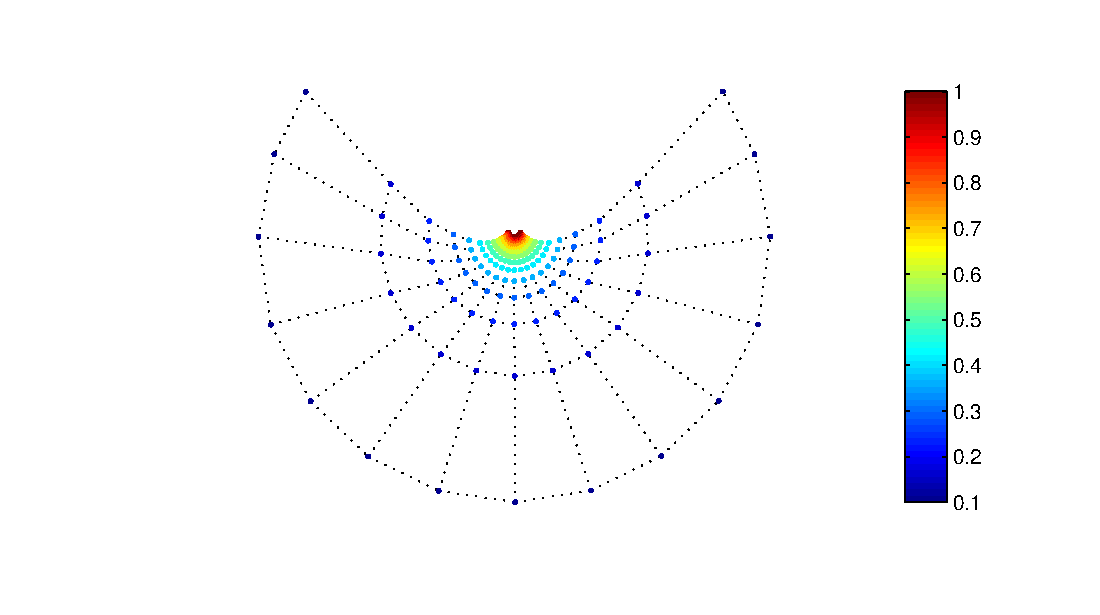
\includegraphics[width=\columnwidth]{figs/embeddings/Normal_KL}
	\caption{Map of Normal distributions on the statistical manifold defined by the log-score, or KL divergence. Dots of the same color show Normal distributions with the same standard deviation. It can be clearly seen that distributions with lower standard deviation are spread out more than those with a higher standard deviation, giving rise to a fan-like structure.}
\end{figure}

\begin{figure}
	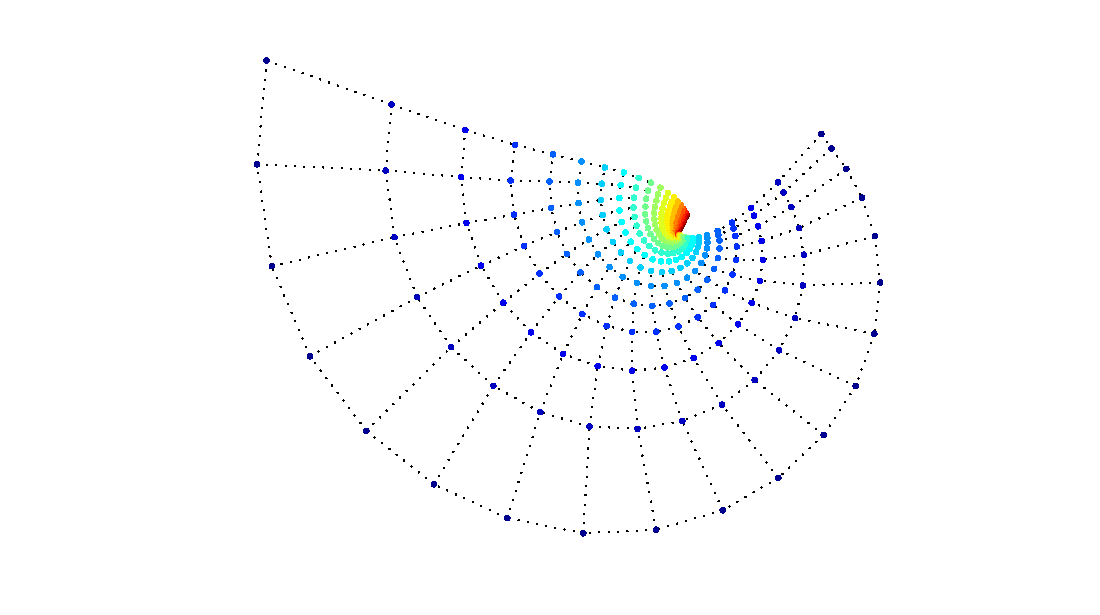
\includegraphics[width=0.45\columnwidth]{figs/embeddings/Gamma_KL_meanvar}
	\hspace{.1\columnwidth}
	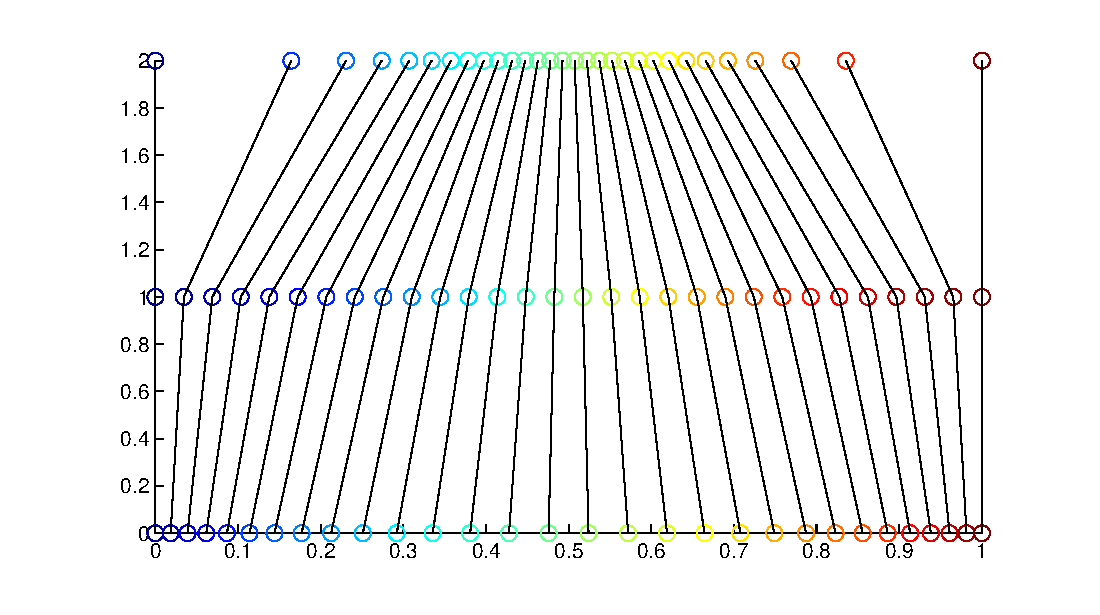
\includegraphics[width=0.45\columnwidth]{figs/embeddings/Normal_KL_nocolorbar}
	\caption{Comparing the statistical manifolds defined by the KL divergence between Gamma \emph{(left)} and Normal \emph{(right)} distributions. Here the mean and variance of each point on the left is matched to the corresponding point on the right (see text for details).  For large values of variance (yellow and red) the two manifolds are very dissimilar, the Gaussian one is symmetric, while the Gamma one is asymmetric. However, as variance decreases (blue), by the central limit theorem Gamma distributions are more alike Gaussians of the same mean and variance, thus the manifold conforms to the fan-like shape that is characteristic of Gaussian distributions.}	
\end{figure}

The most widely used divergence in statistics and machine learning is without doubt the Kullback-Leibler divergence. In his sec I show the geometry it induces on various parametric families of distributions.

Let us start with a very simple, single parameter distribution, the Bernoulli. A Bernoulli distribution describes a binary random variable, where the parameter controls the probability of taking value $1$. In Figure \ref{fig:Bernoulli_manifold} I illustrate the differences between the KL divergence, and the Brier divergence, which corresponds simply to the Euclidean distance between parameter values. As we can see the KL divergence is more sensitive to differences in small (close to 0) and large (close to 1) probabilities, but puts less emphasis on.

When using the KL divergence or the log-score in practical situations, such as in classification, we should therefore expect that much of the statistical power is going to be spent on faithfully matching small probabilities. This is not always desirable: Imagine we were to model the probability that users click on certain news articles on an on-line news website. In this application, most potential clicks have negligible probability, but some user-article combinations may have probabilities closer to $0.5$. If we are to build a recommender system based on this analysis, it is these large probabilities that will be of importance. In this case we are better off using the Brier-score, rather than the log-score which spends serious effort in modelling how small are the small probabilities exactly.

Gaussian distributions are probably the most important family of distributions due to their convenient analytical properties. \TODO{further blah blah about this}
The KL divergence between two univariate Gaussian distributions is available in a closed form and is given by the following formula:

\begin{equation}
	\KL{\Normal_{\mu_1,\sigma_1}}{\Normal_{\mu_2,\sigma_2}} = \frac{\left(\mu_1 - \mu_2\right)^2}{2\sigma_2^2} + \frac{1}{2}\left(\frac{\sigma_1^2}{\sigma_2^2} - 1 - \log\frac{\sigma_1^2}{\sigma_2^2}\right)
\end{equation}


Figure \ref{fig:normals_manifold} illustrates the manifold structure of normal distributions induced by the KL divergence. We can observe that assuming $p$ and $q$ have the same mean, the larger their variance, the easier it becomes to distinguish between them.

We can look at the geometry Shannon's entropy induces within another two-parameter family of continuous distributions, Gamma distributions. Gamma distributions are strictly positive, their probability density function of Gamma distributions is as follows:

\begin{equation}
(x) = \beta^{\alpha}\frac{1}{\Gamma(\alpha)} x^{\alpha-1} \exp(-\beta x)
\end{equation}

where $\alpha,\beta > 0$ are called shape and rate parameters respectively. Special cases of Gamma distributions are exponential distributions when $\alpha=1$.

The KL divergence between Gamma distributions can be computed in closed form and is given by the following formula:

\begin{equation}
	\KL{\Gamma_{\alpha_1,\beta_1}}{\Gamma_{\alpha_2,\beta_2}} = \left(\alpha_1 - \alpha_2\right)\psi\left(\alpha_1\right) - \log\frac{\Gamma(\alpha_1)}{\Gamma(\alpha_2)} + \alpha_1\log\frac{\beta_1}{\beta_2} + \alpha_1\frac{\beta_2 - \beta_1}{\beta_1} \label{eqn:KL_Gamma}
\end{equation}

Figure \ref{fig:Gama_embedding} shows the manifold of Gamma distributions for parameters $a \leq \alpha \leq b, c\leq \beta \leq d$. As we can see this manifold is less symmetric than that of the Gaussians.

For large values of $\alpha$ the standard deviation of the distribution shrinks, and by the central limit theorem, the distribution converges to a Gaussian. We can illustrate this convergence in the manifold structure. For this we first reparametrise the Gamma distribution in terms of its mean and standard deviation. The mean and standard deviation of a Gamma distribution with parameters $\alpha$ and $\beta$ are given by the following formulae:

\begin{align}
	\mu &= \frac{\alpha}{\beta}\\
	\sigma^2 &= \frac{\alpha}{\beta^2}
\end{align}

Solving for $\alpha$ and $\beta$ in these equations we get

\begin{align}
	\alpha &= \frac{\mu^2}{\sigma^2}\\
	\beta &= \frac{\mu}{\sigma^2}
\end{align}

Plugging these into Eqn.\ \eqref{eqn:KL_Gamma} we can now map Gamma distributions with particular mean and variance. Figure 1 compares Normal and Gamma distributions with mean $\mu\in[0.5,1.5]$ and standard deviation $\sigma\in[0.1,1]$. We can observe that as the variance increases, the manifold of Gamma distributions shows a fan-like structure very similarly that of Normal distributions. However, for larger variance, the distributions look less Gaussian, and the manifold becomes more asymmetric. The effect of the central limit theorem would perhaps be even more prominent for smaller values of $\sigma$, but for those cases that case Eqn.\ \eqref{eqn:KL_Gamma} becomes numerically imprecise, as it relies on look-up-table implementation of the Gamma ($\Gamma$) and bigamma ($\psi$) functions.

\subsection{Visualising geometries induced by divergences other than KL}

\begin{figure}
	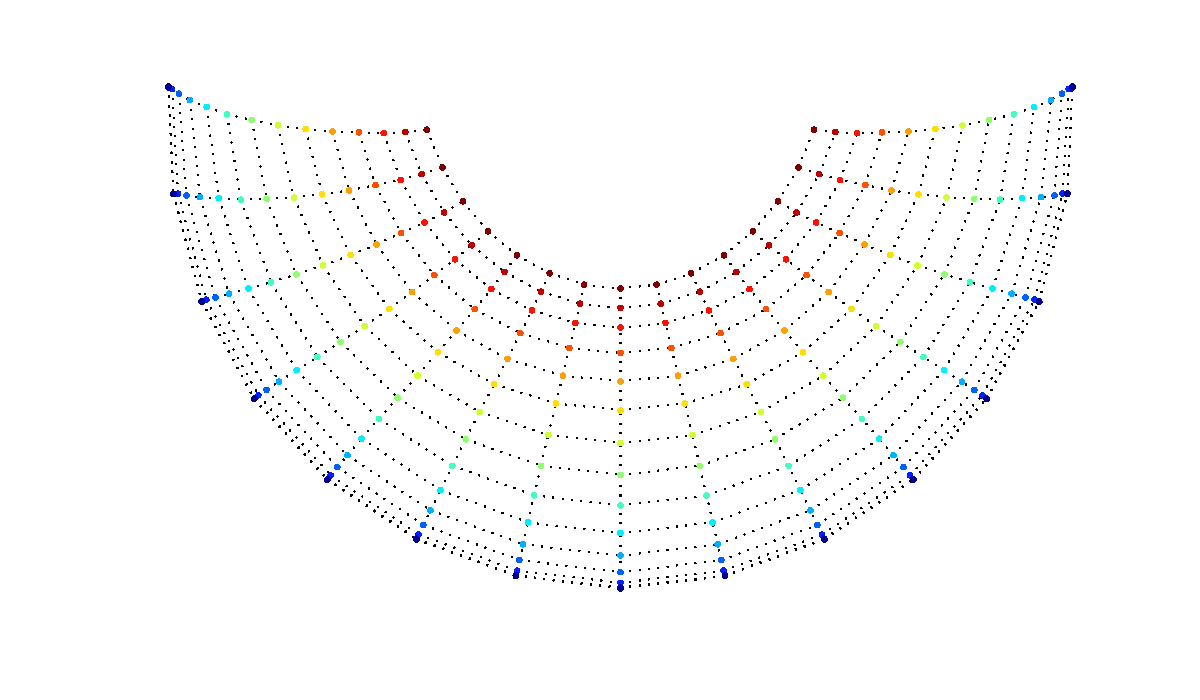
\includegraphics[width=.3\columnwidth]{figs/embeddings/Normal_kernel_1}
	\hspace{0.02\columnwidth}
	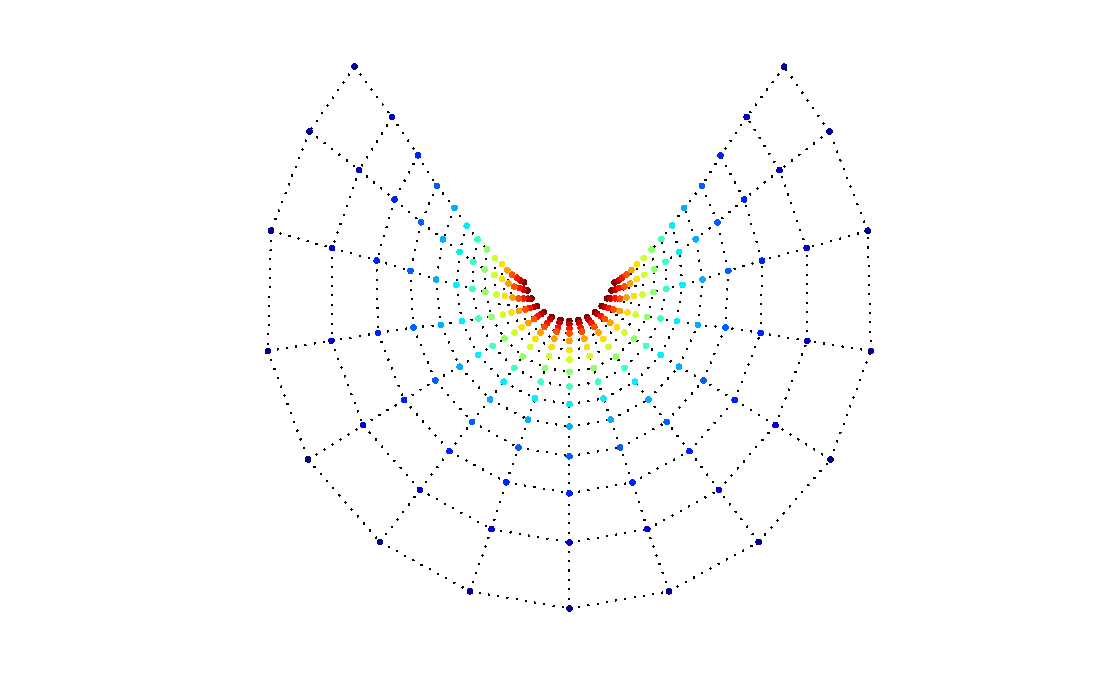
\includegraphics[width=.3\columnwidth]{figs/embeddings/Normal_kernel_2}
	\hspace{0.02\columnwidth}
	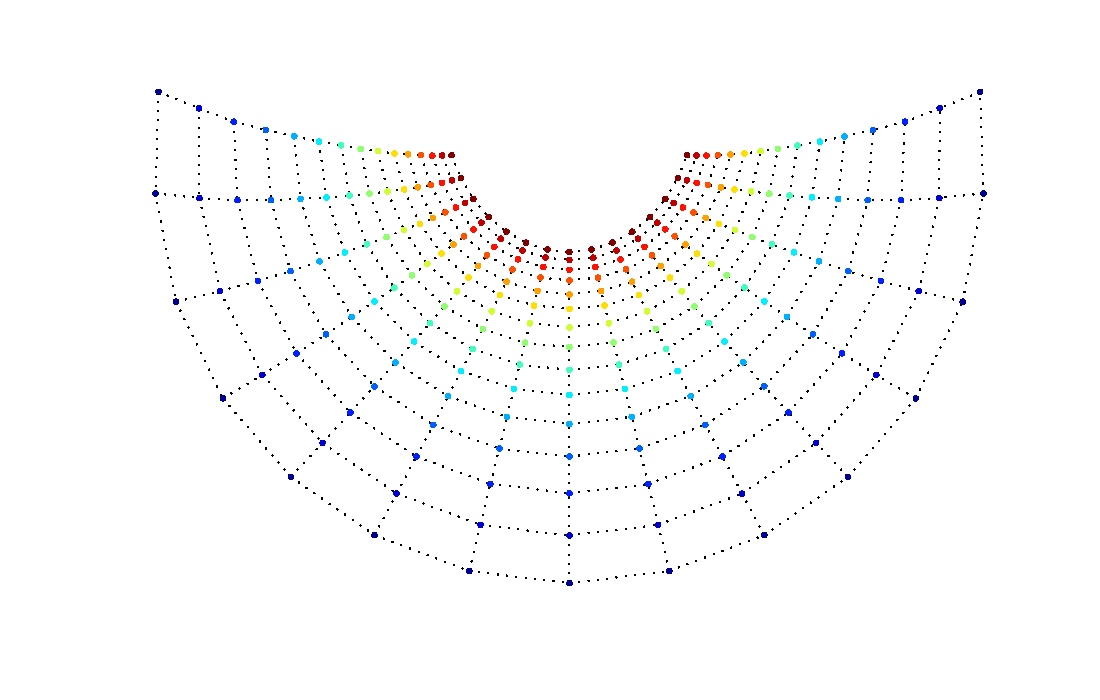
\includegraphics[width=.3\columnwidth]{figs/embeddings/Normal_kernel_3}
	\caption{Map of the statistical manifold corresponding to the kernel score with a square exponential kernel. The lengthscale parameter was set to \emph{(from left to right)} $\ell=0.5,2,5$. For small lengthscales, the divergence is very sensitive to distributions with small standard deviation. As the lengthscale increases, this sensitivity is less and less dominant, and we start to observe comparable resolution amongst distributions with larger variance.}
\end{figure}
The main purpose of this section is to visualise differences between the geometries induced by various divergence measures over the same set of distributions. Here we will mainly focus on Gaussian distributions, as it is analytically convenient to compute various divergences between Gaussians in closed form.

A particularly interesting divergence that we will use in subsequent chapters is that based on the kernel scoring rule, called the MMD (section \ref{sec:kernel_scoring}). The kernel scoring rule itself is very flexible, and its properties are dictated by the choice of kernel function.

For several well-known kernels the MMD between two univariate Gaussians can be computed in closed form. For the squared exponential kernel $k(x,y)=\exp(-\frac{(x-y)^2}{\ell^2})$ the divergence is given by the following formula:

\begin{align}
	\scalar{\mu_{\Normal(\mu_1,\sigma_1)}}{\mu_{\Normal(\mu_2,\sigma_2)}}_{k_{\ell}} = \frac{\ell}{\sqrt{\ell^2 + \sigma_1^2 + \sigma_2^2}}\exp\left(-\frac{(\mu_1 - \mu_2)^2}{2(\ell^2 + \sigma_1^2 + \sigma_2^2)}\right)
\end{align}	

\TODO{correct expression below!!!}

\begin{equation}
	\divergence{k}{\Normal_{\mu_1,\sigma_1}}{\Normal_{\mu_2,\sigma_2}} = \ell\left(\frac{1}{\sqrt{\ell^2+2\sigma_1^2}} + \frac{1}{\sqrt{\ell^2+2\sigma_2^2}} - \frac{2}{\sqrt{\ell^2+\sigma_1^2 + \sigma_2^2}}\exp\left(-\frac{(\mu_1 - \mu_2)^2}{2(\ell^2 + \sigma_1^2 + \sigma_2^2)}\right)\right)
\end{equation}

Figure \ref{fig:Normals_MMD} illustrates the map according to the MMD divergence choosing various values for the lengthscale $\ell$.  \TODO{conclusions} We observe that the structure of the manifold induced by this divergence is qualitatively very similar to that induced by the KL divergence. However, using MMD with the squared exponential kernel allows us the extra flexibility of choosing a characteristic lengthscale, thereby modulating the sensitivity to small differences in variance and mean.

Another widely used kernel is the so-called Laplacian: $k(x,y)=\exp\left(-\frac{\vert x-y\vert}{\ell}\right)$, for which the MMD between Gaussian distributions can still be computed in closed form:

\TODO{find out what the formula is}

Not all scoring rules give rise to smooth manifolds. As an extreme example, consider the following decision problem:

You are uncertain about the temperature of the reactor in a power plant. If the temperature is too high, above a critical temperature $T_{crit}$, the reactor may melt down causing you a loss of \$10 billion. You may choose to shut down the reactor, which costs you \$1 million of lost revenue, irrespective of whether the reactor was indeed overheated or not. You make a probabilistic forecast about the reactor's temperature, and want to make a decision based on that.

This decision rule segments probabilistic forecasts into only two subsets: those which would result in a ``shut down'' decision, and those that result in a ``keep on going''. 

\begin{equation}
	\divergence{reactor}{p}{q} = \left\{
	\begin{array}{cc} 
	    \begin{array}{cc}
	      0        & p(\{t\geq T_{crit}\}) \geq \ell \mbox{ and } q(\{t\geq T_{crit}\}) \geq \ell\\
	      \ell_1 & p(\{t\geq T_{crit}\})  \geq \ell \mbox{ and } q(\{t\geq T_{crit}\}) \leq \ell\\
	      \ell_2 & p(\{t\geq T_{crit}\})  \leq \ell \mbox{ and } q(\{t\geq T_{crit}\}) \geq \ell
	    \end{array}
	\end{array}
	\right.
\end{equation}

This divergence therefore does not give rise to a smooth manifold. Figure \ref{fig two_points} shows a map of Gaussian distributions with respect to the KL divergence. The way $\divergence{reactor}{\cdot}{\cdot}$ segments distributions into ``shut down'' or ``keep on going'' types is also shown. We can make the KL divergence more sensitive to the decision problem at hand by considering a convex combination between $\KL{\cdot}{\cdot}$ and $\divergence{reactor}{\cdot}{\cdot}$.

\chapter{Scoring rules for processes}

\input{part2/scoring_processes}

\chapter{Approximate Bayesian analysis}

%!TEX root = ../main.tex

In practically interesting Bayesian models, the posterior distribution is often computationally intractable to obtain and therefore one has to resort to approximate inference techniques. The most popular approximation methods are variational inference and Markov chain Monte Carlo.

Variational methods operate by minimising an information theoretic divergence between a simple distribution, often of exponential family, and the true posterior. The divergence is often chosen to be a form of Kullback-Leibler divergence, as it allows easy rearrangement of terms and makes local message-passing style computations possible. In section \ref{sec:losscalibrated} argue that when Bayesian inference is performed to solve a particular decision problem, these algorithms are sub-optimal as they are ignorant of the structure of losses. We devised a framework we termed loss-calibrated approximate inference \cite{}, which generalises traditional variational approaches by minimising generalised divergences based on scoring rules. I will demonstrate this framework on a loss-critical toy problem and on a well-known nonparametric Bayesian model, Gaussian process regression.

Monte Carlo methods produce random samples (approximately) drawn from the posterior, which then allow for approximating relevant integrals over the posterior. Monte Carlo techniques are applicable to a wide variety of interesting Bayesian models, and allow for an intuitive trade-off between computation time and accuracy. However, just as most variational approaches, Monte Carlo techniques are also ignorant of the decisions and losses involved in a decision problem. In section \ref{sec:} I introduce a new class of approximate inference algorithms that I call loss-calibrated quasi-Monte Carlo methods. These algorithms produce a deterministic sequence of pseudo-samples in such a way, that the divergence between the empirical distribution of pseudosamples is minimised from the target distribution. I show how kernel herding, a recent algorithm proposed by \cite{kernelherding} can be seen as a special case of loss-calibrated quasi-Monte Carlo, and point out the connection between this method and Bayesian Quadrature.

The work presented in this chapter on loss-calibrated approximate inference and approximate decision theory is joint work with Simon Lacoste-Julien and Zoubin Ghahramani, and most of the results presented here have been published in \cite{losscalibrated}.
The work presented on the equivalence between optimally weighted kernel herding and Bayesian Quadrature is joint work with David Duvenaud, and has been published \cite{losscalibrated}.

\section{Loss-calibrated approximate inference}

\TODO{General paragraph about Bayesian inference}

In many practically relevant cases computing the posterior is not analytically tractable. This is predominantly due to the fact that the integral defining the marginal likelihood $\int p(\dataset\vert\theta)p(\theta)d\theta$ cannot be computed analytically in closed form, and therefore the normalisation of the posterior cannot be computed. But sometimes the complexity of evaluating even the unnormalised posterior increases exponentially with the amount of observed data, as in the case of for example switching state space models. In either case, it is usual practice to approximate the intractable posterior by something simpler, an approximate distribution $q$. The problem of finding an approximate posterior $q$ is referred to as approximate inference.

Over the years, two dominant branches of approximate inference emerged. The first branch, that I will refer to as parametric approximation schemes, includes variational inference, Laplace approximation and expectation propagation. The common theme in these techniques is that the complicated posterior is replaced by an approximate distribution chosen from a particular parametric family of distributions, usually from an exponential family. These methods differ in their objective functions they minimise, which measure discrepancy between the target posterior distribution and the approximation $q$.

\subsection{Overview of variational methods and expectation propagation}

Variational methods to approximate inference find the optimal approximation $q^{*}$ to the posterior by maximising a lower bound to the marginal likelihood as follows.

\begin{align}
	\log p(\dataset) &= \log \int p(\dataset\vert\theta)p(\theta) d\theta\\
		&=\log \int \frac{p(\dataset\vert\theta)p(\theta)}{q(\theta)}q(\theta) d\theta\\
		&\geq \int \log \frac{p(\dataset\vert\theta)p(\theta)}{q(\theta)} q(\theta) d\theta\\
		&= \log p(\dataset) - \KL{p_{\dataset}}{q}
\end{align}

by minimising the Kullback-Leibler divergence (Eqn.\ \eqref{eqn:KL_divergence}) between the approximate distribution $q$ and the true posterior $p_{\dataset}$. A common practice in approximate inference is to choose the approximate posterior distribution $q$ from an exponential family of distributions $\Qe$, and it is also often common practice to choose $q$ such that it factorises over multivariate quantities. When these assumptions are made, the solution to the above optimisation can often be expressed in closed form, or efficient iterative algorithms exist for finding a locally optimal solution numerically.

The KL divergence is non-symmetric, therefore the order of arguments matter. Variational methods minimise $\KL{q}{p_{\dataset}}$, that is with the approximate distribution being the first argument. On the one hand, this is highly convenient as computing the divergence in this direction requires integration only over $q$, which is assumed simpler than the real posterior $p_{\dataset}$.On the other hand, as I argued in section \ref{sec:scoring_rules}, in the scoring rule interpretation suggests that the \emph{right} way to use divergence is $\KL{p_{\dataset}}{q}$, i.\,e.\ when its first argument is the true distribution we want to approximate, and the second argument some approximation $q$. This has been pointed out previously by \cite{Csato2002,Minka2001} and many other authors. This does not mean that variational inference does not work, it just means that by performing variational inference we loose some of the intuitive interpretation of KL divergence as Bregman divergence under the logarithmic loss.

Several approaches therefore tried to fix this conceptual issue, and minimise KL divergence in the opposite direction. This is unfortunately a challenge, as computing the divergence $\divergence{\score}{p_{\dataset}}{q}$ always requires an integral over the posterior $p_{\dataset}$, which is normally intractable, and this is why we perform approximate inference in the first place.

Assumed density filtering, and its generalisation, expectation propagation (EP) try to approximate the ideal method of minimising $\KL{p_{\dataset}}{q}$ as follows. EP assumes the posterior can be written as a product of factors as such:

\begin{equation}
	p_{\dataset}(\theta) = \frac{1}{Z} \prod t_i(\theta)
\end{equation}

The terms $t_i$ are assumed simple, and in most cases depend only on a few components of the multivariate parameter vector $\theta$. What makes the posterior intractable is the normalisation constant $Z$, computing which would involve a very expensive integral. Expectation propagation approximates the posterior by substituting approximate factors $\tilde{t}_i$ for original factors $t_i$, in such a way that the product of approximate factors

\begin{equation}
	q(\theta) = \prod \tilde{t}_i(\theta)
\end{equation}

is tractable. The approximate factors are improved one-by-one using the following objective function:

\begin{equation}
	\tilde{t}_i^{new} = \argmin_{t \in \text{approximate family}} \KL{\frac{1}{\int q(\theta)\frac{t_i(\theta)}{\tilde{t}_i(\theta)} d\theta}q(\theta)\frac{t_i(\theta)}{\tilde{t}_i(\theta)}}{q(\theta)\frac{t_i(\theta)}{t(\theta)}}
\end{equation}

Essentially, in each iteration the algorithm replaces one of the approximate factors in the approximate posterior $q$ with the real factor to construct a one-step-closer-to-exact approximation to the posterior $\tilde{q}$. Then it uses this $\tilde{q}$ as the target distribution and computes a new approximation by minimising KL divergence. This step is repeated until convergence, that is until no approximate factors can be further improved by the KL divergence metric.

Thus in expectation-propagation, the KL divergence is used in the right direction that is well motivated by the theory of scoring rules and Bregman divergences. However, as computing KL divergence in the right direction is intractable it has to use a roundabout method.

\subsection{Loss-calibrated approximate inference}

Although often overlooked, the main theoretical motivations for the Bayesian paradigm are rooted in Bayesian decision theory~\cite{berger85decision}, which provides a well-defined theoretical framework for rational decision making under uncertainty about a hidden parameter $\theta$. Approximate inference is concerned with approximating the posterior, but often ignores the fact that the posterior is then used in a wider context to make optimal decisions. In this section I review the theory of Bayesian decisions, and then devise a framework for addressing questions that arise when using approximate inference in the context of optimal decision making.

The ingredients of Bayesian decision theory are (see Ch.~2 of~\cite{robert01choice} or Ch.~1 of~\cite{berger85decision} for example):
\vspace{-.3cm}
\begin{itemize}
  \item a loss $\loss(\theta,\action)$ which quantifies the cost of taking action $\action \in \actionset$ when the world state is $\theta \in \Theta$; %\footnote{Note that $\theta$ is not assumed to be finite dimensional; in the most general setting, it could fully specify an arbitrary distribution over $\mathcal{O}$.};
  \item an observation model $p(\dataset|\theta)$ which gives the probability of observing some data or dataset $\dataset \in \mathcal{O}$ assuming that the world state is $\theta$;
  \item a prior belief $p(\theta)$ over world states.
\end{itemize}

The loss $\loss$ describes the decision task that we are interested in, whereas the observation model and the prior represent our beliefs about the world. Given these components, the ultimate objective for evaluating a possible action $\action$ after observing $\dataset$ is the \emph{expected posterior loss} (also called the \emph{posterior risk}~\cite{schervish95theory})

\begin{equation}
	\risk_{p_\dataset}(\action) \doteq \int_\Theta \loss(\theta, a) \, p(\theta|\dataset) d\theta
\end{equation}

In the Bayesian framework, the optimal action $\action_{p_\dataset}$ is the one that minimizes $\risk_{p_\dataset}$.

In this framework it is therefore easy to see that Bayesian decision making decomposes into two consecutive steps of computation. First, a posterior $p_\dataset$ is inferred from observed data $\dataset$, then the optimal action is selected by minimising risk under this posterior. Crucially, the first step is independent of losses, the posterior can be computed irrespective of how the loss $\loss$ is defined. In fact, once we have computed the posterior, the same distribution can be used to solve different decision problems with different losses involved. This independent breakdown of computation is what makes the posterior distribution such an important object in Bayesian statistics.

But when the posterior is intractable to compute and approximations are needed - as it is the case most of the time - additional questions arise. Is this two-step breakdown of computations to inference and then risk minimisation still a sensible thing to do? How should we decide what approximate inference method to use? Can we still re-use the same approximate posterior with different loss functions just as we can if no approximations are needed. Is the choice of approximate inference technique independent of the loss function? This chapter introduces loss-calibrated approximate Bayesian inference is a theoretical framework for addressing these questions.

To illustrate the role and behaviour ot approximate inference in a Bayesian decision problem consider the following simple problem. Suppose that we control a nuclear power-plant which has an unknown temperature $\theta$ that we model with Bayesian inference based on some measurements $\mathcal{D}$.
The plant is in danger of over-heating, and as the operator, we can take two actions: either shut it down or keep it running. Keeping it running while the temperature is above a critical threshold $T_\mathrm{crit}$ will cause a nuclear meltdown, incurring a large loss $L(\theta>T_\mathrm{crit},\mbox{'on'})$. On the other hand, shutting down the power plant incurs a moderate loss $L(\mbox{'off'})$, irrespective of the temperature. 
%Given our posterior $p_\dataset$ and the losses, we want to compute the Bayes-optimal action that minimizes the posterior risk. 
Suppose that our current observations yielded a complicated multi-modal posterior $p_\dataset(\theta)$ (\ref{fig:toy}, solid curve) that we do not have comutational resources to represent. Thus we chose to approximate it with a simple Gaussian distribution.

Now consider how various approaches to approximate inference would perform in terms of their Bayesian posterior risk. Minimizing $\KL{q}{p_\dataset}$, as in variational inference, yields candidate $q_1$ which concentrates around the largest mode, ignoring entirely the second small mode around the critical temperature \ref{fig:toy}, dotted curve). Minimizing $\KL{p_\dataset}{q}$ gives a more global approximation: $q_2$ matches moments of the posterior, but still underestimates the probability of the temperature being above $T_\mathrm{crit}$, thereby leading to a suboptimal decision \ref{fig:toy}, dashed curve).

\TODO{Rewrite as divergences have not been definded yet} $q_3$ is one of the minimizers of $d_L(p_\dataset \| q)$ in this setting, resulting in the same decision as $p_\dataset$ \ref{fig:toy}, dash-dotted curve). Note that $q_3$ does not model all aspects of the posterior, but it estimates the Bayes-decision well. Because there are only two possible actions in this setup, the set $\mathcal{Q}$ is split in only two halves by the function $d_L(p_\dataset,q)$ and so there are infinitely many $q_\mathrm{opt}$'s that are equivalent in terms of their risk. In contrast, in the predictive setting of section~\ref{ss:predictive} where in addition we assume $\mathcal{X}$ and $p(x)$ to be continuous, we could obtain a finer resolution $d_L(p_\dataset \| q)$ which can potentially yield a unique optimizer.

This simple example already highlighted some features of the loss-calibrated framework. First of all, it is clear, that even in a simple example the choice of approximate inference methods matters, and has a great influence on risks and the final decisions made. In this case minimising $\KL{p_\dataset}{q}$ yielded a solution superior to minimising the variational criterion $\KL{q}{p_\dataset}$, but we could just as well construct another example, where it is the other way around. Even though $\KL{p_\dataset}{q}$ is thought of as the more principled method, in the context of this decision problem neither of them is clearly better or more principled than the other.

\subsection{The loss-calibrated approximate inference framework}

In practice, one usually treats the approximate $q$ as if it was the true posterior and chooses the action that minimizes what we will call the \emph{$q$-risk}:
\begin{equation} \label{e:q-risk}
    \mathcal{R}_q(h) \doteq \int_\Theta q(\theta) L(\theta,h) d\theta ,
\end{equation}
obtaining a \emph{$q$-optimal} action $h_q$:
\begin{equation}
    h_q \doteq \argmin{h \in \mathcal{H}} \mathcal{R}_q(h).
\end{equation}
In this paper, we will assume that computing exactly the $q$-optimal action $h_q$ for $q \in \mathcal{Q}$ is tractable, and focus on the problem of choosing a suitable $q$ to approximate the posterior $p_\dataset$ \emph{in order to yield a decision $h_q$ with low posterior risk $\mathcal{R}_{p_\dataset}(h_q)$}, mimicking the standard methodology but crystallizing the decision theoretic goal. Given this approach, a (usually non-unique) optimal $q \in \mathcal{Q}$ is clearly:
\begin{equation}
    q_\mathrm{opt} = \argmin{q \in \mathcal{Q}} \mathcal{R}_{p_\dataset}(h_q),
\end{equation}
though a practical algorithm might only be able to find an approximate minimizer to this quantity. In the case where $p_\dataset\in\mathcal{Q}$, $p_\dataset$ is obviously optimal according to this criterion.

We could interpret the above criterion as minimizing the following asymmetric non-negative discrepancy measure between distributions:
\begin{equation} \label{e:d_L}
    d_L(p\|q) \doteq \mathcal{R}_{p}(h_q) - \mathcal{R}_{p}(h_p).
\end{equation}
Interestingly, the Kullback-Leibler divergence $KL(p\|q)$ can be interpreted as a special case of $d_L$ for the task of posterior density estimation over $\Theta$. In this task, an action $h$ is a density over $\Theta$ and the standard density estimation statistical loss is $L(\theta,h) = -\log h(\theta)$. The $q$-risk $R_q(h)$ then becomes the cross-entropy $H(q,h)=-\int_\Theta q(\theta) \log(h(\theta)) d\theta$, and so $h_q = q$ assuming that $q \in \mathcal{H}$. Under these assumptions, we obtain that $KL(p\|q) = d_L(p\|q)$ and so as was already known in statistics, $KL(p_\dataset\|\cdot)$ appears ``loss-calibrated'' for the task of posterior density estimation in our approximation framework. But this begs the natural question of whether minimizing $d_L$ for a particular loss $L$ provides optimal performance under other losses. We will show in \ref{ss:GPR} that even in the simple Gaussian linear regression setting, minimizing the KL divergence can be suboptimal in the squared loss sense, thus motivating us to seek loss-calibrated alternatives.

\paragraph{Example: Gaussian process regression}

In this case we do not actually need to perform approximate inference, as the posterior is Gaussian and available in closed form. However it allows us to express the quantities relevant for loss-calibrated approximate inference.
§
Gaussian process regression.

\section{Loss-calibrated quasi-Monte-Carlo}

\paragraph{Monte Carlo - about two paragraphs}
A popular alternative to parametric approximation schemes, such as variational inference and expectation propagation are Monte Carlo methods.

Monte Carlo methods produce random samples from the posterior distribution $p_\dataset$ and then approximate relevant integrals by taking the empirical means over these samples. Subject to smoothness conditions, this non-deterministic estimate of any integral converges at a rate $\mathcal{O}(\frac{1}{\sqrt{N}})$, where $N$ is the number of samples. This convergence is guaranteed by the law of large numbers. An appealing property of Monte Carlo methods is that in theory an arbitrarily precise estimate can be obtained by just increasing the number of samples. In this sense, Monte Carlo approximation is non-parametric: the number of parameters that describe the approximate distribution is not fixed ahead of time, and can be arbitrarily large.

When exact sampling from $p_\dataset$ is impossible or impractical, Markov chain Monte Carlo (MCMC) methods are often used. MCMC methods only require knowing the target distribution up to a constant factor. Practically this means that even if the normalisation constant of the posterior is intractable, MCMC techniques can still be used to generate samples from it.

Various variants of MCMC methods can be applied to almost any problem but the convergence rate of the estimate depends on several factors and is hard to estimate \citep{CowlesCarlin96}. Typically, MCMC techniques introduce positive correlation between subsequent samples, and thus are less effective than exact Monte Carlo sampling. For an overview of various Monte Carlo techiques, see \citep{Murray2007}.

Monte Carlo methods are very general, they guarantee convergence for any measurable integral. Hence, convergence is also guaranteed in the KL divergence sense, and as the posterior risk is expressed as an integral, they also ensure convergence in $d_\loss(\cdot\|\cdot)$ for any loss function $\ell$. However, the rate of convergence cannot be fine-tuned to a particular divergence measure. One might hope that if the loss function $\ell$ is known ahead of time, a faster convergence rate can be achieved, maybe at the cost of slowing down convergence on integrals that are irrelevant to the decision problem.

\paragraph{revisit toy example} Let us consider the power plant example from the previous section. To be able to make a decision, the only thing we need to know is the probability of the temperature exceeding the critical temperature. Thus, when the distribution is approximated via Monte Carlo, the only summary statistic we care about is the fraction of samples that are above the critical temperature.

The probability of interest can be written as the expectation of the indicator function that takes value $1$ if the temperature exceeds the critical one and $0$ otherwise. This indicator function is measurable, therefore an $\mathcal{O}(\frac{1}{\sqrt{N}})$ convergence is guaranteed by exact MCMC sampling.
However, it is easy to construct an ideal series of $N$ `pseudo-samples' where the error is upper bounded by $\frac{1}{N}$. (The problem is equivalent to approximating the probability with a series of rational numbers). This ideal set of $N$ pseudosamples may of course be a terrible general approximation to the full probability distribution $p_\dataset$, but from the perspective of the decision problem it converges much faster than the random Monte Carlo samples.

\TODO{illustrate this on figures: Fig 1: same as in previous section. Fig 2: approximating the probability with random MCMC and with optimal QMC}

\paragraph{Quasi monte Carlo approaches}

 The focus of this chapter are quasi-Monte Carlo methods that -- instead of sampling randomly -- produce a set of pseudo-samples in a deterministic fashion. These methods operate by directly minimising some sort of discrepancy between the empirical distribution of pseudo-samples and the target distribution. Whenever these methods are applicable, they achieve convergence rates superior to the $\mathcal{O}(\frac{1}{\sqrt{N}})$ rate typical of random sampling.

TODO{review existing quasi-Monte-Carlo methods: Sobol sequences, Halton sequence}

The quasi-Monte-Carlo methods reviewed here often achieve faster convergence rates than traditional random Monte Carlo, but they are general-purpose sampling tools: they cannot be fine-tuned to particular decision problems we may want to use them for. Here I will introduce a class of quasi-Monte-Carlo methods that I will call loss-calibrated QMC. 

Quasi-Monte-Carlo can be interpreted as a special case of approximate inference, where the approximating family is the family of empirical distributions
\begin{equation}
	q(x ; x_1,\ldots,x_N) = \frac{1}{N} \sum_{n=1}^{N} \delta(x - x_n)\mbox{,}
\end{equation}
or weighted empirical distributions
\begin{equation}
	q(x ; x_1,\ldots,x_N,w_1,\ldots,w_N) = \sum_{n=1}^{N} w_n \delta(x - x_n)\mbox{.}
\end{equation}

Finding the optimal loss-calibrated sample set can then be achieved by minimising the loss-calibrated divergence $d_\loss$ between the target distribution $p_\dataset$ and the approximation $q$:

\begin{equation}
	\{x_1,\ldots,x_N\}_{n=1}^{N} = \argmin_{\{x_1,\ldots,x_N\}_{n=1}^{N}} \divergence{\loss}{p_\dataset}{q(x ; x_1,\ldots,x_N)} \label{eqn:loss_calibrated_nonsequential}
\end{equation}
It is important to note, that the above procedure does not make sense for general Bregman divergences. For example, the KL divergence $\KL{p}{q}$ requires the approximate distribution $q$ to be absolutely continuous with respect to the target distribution $p$, which, unless the target distribution is also discrete, cannot be satisfied if $q$ is atomic.

The minimisation in Equation \eqref{eqn:loss_calibrated_nonsequential} is 
\paragraph{Myopic sequential loss-calibrated Quasi Monte Carlo}


In most cases - just as loss-calibrated approximate inference in general, algorithmic implementations of loss-calibrated QMC requires the ability to evaluate certain integrals over the target distribution easily, therefore practical applications of loss-calibrated QMC in the form presented here are limited. Nevertheles, the framework may provide useful blueprint for designing sampling algotithms that are more tailored to particular decision scenarios.

%!TEX root = ../main.tex
\definecolor{mydarkblue}{rgb}{0,0.08,0.45}

\begin{figure}[h]
\centering
\includegraphics[width=\columnwidth]{figs/herding/fig1_v2}
\caption{The first 8 samples from sequential Bayesian quadrature, versus the first 20 samples from herding.  Only 8 weighted \sbq{} samples are needed to give an estimator with the same maximum mean discrepancy as using 20 herding samples with uniform weights.  Relative sizes of samples indicate their relative weights.}
\label{fig:fig1}
\end{figure} 

\subsubsection{INTRODUCTION}
\paragraph{The problem: Integrals} A common problem in statistical machine learning is to compute expectations of functions over probability distributions of the form:
\begin{equation}
	Z_{f,p} = \int f(x) p(x) dx \label{eqn:integral}
\end{equation}
Examples include computing marginal distributions, making predictions marginalizing over parameters, or computing the Bayes risk in a decision problem. In this paper we assume that the distribution $p(x)$ is known in analytic form, and $f(x)$ can be evaluated at arbitrary locations.

Monte Carlo methods produce random samples from the distribution $p$ and then approximate the integral by taking the empirical mean $\hat{Z} = \frac{1}{N}\sum_{n=1}^{N}f_{x_n}$ of the function evaluated at those points. This non-deterministic estimate converges at a rate $\mathcal{O}(\frac{1}{\sqrt{N}})$. When exact sampling from $p$ is impossible or impractical, Markov chain Monte Carlo (MCMC) methods are often used. MCMC methods can be applied to almost any problem but convergence of the estimate depends on several factors and is hard to estimate \citep{CowlesCarlin96}. The focus of this paper is on quasi-Monte Carlo methods that -- instead of sampling randomly -- produce a set of pseudo-samples in a deterministic fashion. These methods operate by directly minimising some sort of discrepancy between the empirical distribution of pseudo-samples and the target distribution. Whenever these methods are applicable, they achieve convergence rates superior to the $\mathcal{O}(\frac{1}{\sqrt{N}})$ rate typical of random sampling.

In this paper we highlight and explore the connections between two deterministic sampling and integration methods: Bayesian quadrature (\bq{}) \citep{BZHermiteQuadrature,BZMonteCarlo} (also known as Bayesian Monte Carlo) and kernel herding \citep{chen2010super}. Bayesian quadrature estimates integral \eqref{eqn:integral} by inferring a posterior distribution over $f$ conditioned on the observed evaluations $f_{x_n}$, and then computing the posterior expectation of $Z_{f,p}$. The points where the function should be evaluated can be found via Bayesian experimental design, providing a deterministic procedure for selecting sample locations.

Herding, propositionosed recently by \cite{chen2010super}, produces pseudosamples by minimising the discrepancy of moments between the sample set and the target distribution. Similarly to traditional Monte Carlo, an estimate is formed by taking the empirical mean over samples $\hat{Z} = \frac{1}{N}\sum_{n=1}^{N}f_{x_n}$. Under certain assumptions, herding has provably fast, $\mathcal{O}(\frac{1}{N})$ convergence rates in the parametric case, and has demonstrated strong empirical performance in a variety of tasks.

\paragraph{Summary of contributions} In this paper, we make two main contributions.  First, we show that the Maximum Mean Discrepancy (MMD) criterion used to choose samples in kernel herding is identical to the expected error in the estimate of the integral $Z_{f,p}$ under a Gaussian process prior for $f$.  This expected error is the criterion being minimized when choosing samples for Bayesian quadrature.  Because Bayesian quadrature assigns different weights to each of the observed function values $f(\vx)$, we can view Bayesian quadrature as a weighted version of kernel herding.  We show that these weights are optimal in a minimax sense over all functions in the Hilbert space defined by our kernel.  This implies that Bayesian quadrature dominates uniformly-weighted kernel herding and other non-optimally weighted herding in rate of convergence.

Second, we show that minimising the MMD, when using \bq{} weights is closely related to the sparse dictionary selection problem studied in \citep{KrauseCevher10}, and therefore is approximately submodular with respect to the samples chosen. This allows us to reason about the performance of greedy forward selection algorithms for Bayesian Quadrature. We call this greedy method Sequential Bayesian Quadrature (\sbq{}).

We then demonstrate empirically the relative performance of herding, i.i.d random sampling, and \sbq{}, and demonstrate that \sbq{} attains a rate of convergence faster than $\mathcal{O}(1/N)$.



\subsubsection{HERDING} 

Herding was introduced by \cite{welling2009herding} as a method for generating pseudo-samples from a distribution in such a way that certain nonlinear moments of the sample set closely match those of the target distribution.  The empirical mean $\frac{1}{N}\sum_{n=1}^{N}f_{x_n}$ over these pseudosamples is then used to estimate integral \ref{eqn:integral}.

\subsubsection{Maximum Mean Discrepancy}

For selecting pseudosamples, herding relies on an objective based on the maximum mean discrepancy \citep[MMD;\ ][]{Sriperumbudur2010}. MMD measures the divergence between two distributions, $p$ and $q$ with respect to a class of integrand functions $\mathcal{F}$ as follows:
%
\begin{align}
	\div{\Fe}{p}{q} = \sup_{f\in\Fe}\left\vert\int f(x) p(x) dx - \int f(x) q(x) dx \right\vert
\end{align}

Intuitively, if two distributions are close in the MMD sense, then no matter which function $f$ we choose from $\mathcal{F}$, the difference in its integral over $p$ or $q$ should be small. A particularly interesting case is when the function class $\mathcal{F}$ is functions of unit norm from a reproducing kernel Hilbert space (RKHS) $\He$. In this case, the MMD between two distributions can be conveniently expressed using expectations of the associated kernel $k(x, x')$ only \citep{Sriperumbudur2010}:
%
\begin{align}
MMD^2_{\He}(p,q) =& \sup_{\substack{f\in\He\\\Hnorm{f}=1}}\left\vert\int f_x p(x) dx - \int f_x q(x) dx\right\vert^2\label{eqn:rkhs-mmd}\\
	=& \Hnorm{\mu_{p} - \mu_{q}}^2\\
\nonumber	=&\iint k(x,y) p(x) p(y) dx dy\\
\nonumber	-2 &\iint k(x,y) p(x) q(y) dx dy\\
	+ &\iint k(x,y) q(x) q(y) dx dy,
\end{align}
%
where in the above formula $\mu_{p}=\int \phi(\vx)p(\vx)d\vx\in\He$ denotes the \emph{mean element} associated with the distribution $p$. For characteristic kernels, such as the Gaussian kernel, the mapping between a distribution and its mean element is bijective. As a consequence $\mmd_{\He}(p,q)=0$ if and only if $p=q$, making it a powerful measure of divergence.

Herding uses maximum mean discrepancy to evaluate of how well the sample set $\{\vx_1,\ldots,\vx_{N}\}$ represents the target distribution $p$:

\begin{align}
	\epsilon_{herding}&\left(\{\vx_1,\ldots,\vx_{N}\}\right) = \mmd_{\He}\left(p,\frac{1}{N}\sum_{n=1}^{N}\delta_{x_n}\right)\\
\nonumber	=&\iint k(x,y) p(x) p(y) dx dy\\
		-2 &\frac{1}{N}\sum_{n=1}^{N}\int k(x,x_n) p(x) dx
		+ \frac{1}{N^2}\sum_{n,m=1}^{N} k(x_n,x_m)
\label{eq:mmd_assumption}
\end{align}
%
The herding procedure greedily minimizes its objective $\epsilon_{herding}\left(\{\vx_1,\ldots,\vx_{N}\}\right)$ , adding pseudosamples $\vx_n$ one at a time. When selecting the $n+1$-st pseudosample:
%
\begin{align}
\vx_{n+1} &\leftarrow \argmin_{\vx \in \mathcal{X}} \label{eqn:herding_criterion} \epsilon_{herding}\left(\{\vx_1,\ldots,\vx_{n},\vx\}\right)\\
	&= \argmax_{\vx \in \mathcal{X}} 2 \expect{\vx' \sim p}{k(\vx, \vx')} - \frac{1}{n+1}\sum_{m=1}^{n} k(\vx,\vx_m)\mbox{,}\notag
\end{align}
%
assuming $k(\vx,\vx) = \mbox{const}$.
The formula \eqref{eqn:herding_criterion} admits an intuitive interpretation: the first term encourages sampling in areas with high mass under the target distribution $p(\vx)$.  The second term discourages sampling at points close to existing samples. 

Evaluating \eqref{eqn:herding_criterion} requires us to compute $\expect{\vx' \sim p}{k(\vx, \vx')} $, that is to integrate the kernel against the target distribution. Throughout the paper we will assume that these integrals can be computed in closed form. Whilst the integration can indeed be carried out analytically in several cases \citep{Song2008,chen2010super}, this requirement is the most pertinent limitation on applications of kernel herding, Bayesian quadrature and related algorithms.

\subsubsection{Complexity and Convergence Rates}

Criterion \eqref{eqn:herding_criterion} can be evaluated in only $\mathcal{O}(n)$ time. Adding these up for all subsequent samples, and assuming that optimisation in each step has $\mathcal{O}(1)$ complexity, producing $N$ pseudosamples via kernel herding costs $\mathcal{O}(N^2)$ operations in total.

In finite dimensional Hilbert spaces, the herding algorithm has been shown to reduce $\mmd$ at a rate $\mathcal{O}(\frac{1}{N})$, which compares favourably with the $\mathcal{O}(\frac{1}{\sqrt{N}})$ rate obtained by non-deterministic Monte Carlo samplers. However, as pointed out by \cite{bach2012equivalence}, this fast convergence is not guaranteed in infinite dimensional Hilbert spaces, such as the RKHS corresponding to the Gaussian kernel.




\subsubsection{BAYESIAN QUADRATURE} 

\begin{figure}
\centering
\includegraphics[width=\columnwidth]{figs/herding/bq_intro4}
\caption{An illustration of Bayesian Quadrature.  The function $f(x)$ is sampled at a set of input locations.  This induces a Gaussian process posterior distribution on $f$, which is integrated in closed form against the target density, $p(\vx)$.  Since the amount of volume under $f$ is uncertain, this gives rise to a (Gaussian) posterior distribution over $Z_{f,p}$.}
\label{fig:bq_intro}
\end{figure}

So far, we have only considered integration methods in which the integral \eqref{eqn:integral} is approximated by the empirical mean of the function evaluated at some set of samples, or pseudo-samples.  Equivalently, we can say that Monte Carlo and herding both assign an equal $\frac{1}{N}$ weight to each of the samples.

In \citep{BZMonteCarlo}, an alternate method is propositionosed: Bayesian Monte Carlo, or Bayesian quadrature (\bq).  \bq{} puts a prior distribution on $\vf$, then estimates integral \eqref{eqn:integral} by inferring a posterior distribution over the function $\vf$, conditioned on the observations $\vf(\vx_n)$ at some query points $\vx_n$.  The posterior distribution over $f$ then implies a distribution over $Z_{f,p}$.  This method allows us to choose sample locations $\vx_n$ in any desired manner. See Figure \ref{fig:bq_intro} for an illustration of Bayesian Quadrature.

%In \cite{BZMonteCarlo}, an alternate method was propositionosed: Bayesian Monte Carlo, or Bayesian quadrature (\bq).  \bq{} puts a prior distribution on $\vf$, then conditions on the observations $\vf(\vx_n)$ to obtain a posterior distribution over the function $\vf$.  The posterior over $\vf$ then implies a Then estimates integral \eqref{eqn:integral} by 


\subsubsection{ BQ Estimator}

Here we derive the \bq{} estimate of \eqref{eqn:integral}, after conditioning on function evaluations $\vf(\vx_1) \dots \vf(\vx_N)$, denoted as $f(\vX)$.  The Bayesian solution implies a distribution over $Z_{f,p}$.  The mean of this distribution, $\expect{}{Z}$ is the optimal Bayesian estimator for a squared loss.

For simplicity, $\vf$ is assigned a Gaussian process prior with kernel function $k$ and mean $0$.  This assumption is very similar to the one made by kernel herding in Eqn.\ \eqref{eq:mmd_assumption}.

After conditioning on $\vf_{\vx}$, we obtain a closed-form posterior over $\vf$:
%
\begin{align}
p(\vf(\vx\st)|\vf(\vX)) = \Normal{\vf_{\vx\st}}{\mf(\vx\st)}{\cov(\vx\st,\vx\st')}
\end{align} 
where
\begin{align}
\mf(\vx\st) = & k(\vx\st, \vX) K^{-1} \vf(\vX) \\
\cov(\vx\st, \vx\st') = & k(\vx\st,\vx\st) - k(\vx\st, \vX) K^{-1} k(\vX, \vx\st)
\end{align} 
%
and $K = k(\vX, \vX)$. 
%
Conveniently, the \gp{} posterior allows us to compute the expectation of \eqref{eqn:integral} in closed form: 
%
%\begin{align}
%Z & = \int f(\vx)p(\vx)d\vx
%\end{align} 
%so we integrate over functions to get:
\begin{align}
\expect{\gp}{Z} & = \expect{\gp}{\int f(\vx)p(\vx)d\vx}\\
 & = \int\!\!\! \int\!\! f(\vx) p(f(\vx)|\vf(\vX)) p(\vx) d\vx df\\
 & = \int\!\!\! \mf(\vx) p(\vx) d\vx \\
 & = \left[ \int\!\! k(\vx, \vX) p(\vx) d\vx \right] K^{-1} \vf(\vX) \\
 & = \vz^T K^{-1} \vf(\vX)
\label{eq:marg_mean_symbolic}
\end{align} 
where
\begin{align}
z_n & = \int\!\! k(\vx, \vx_n) p(\vx) d\vx = \expect{\vx' \sim p}{k(\vx_n, \vx')}.
\end{align}
%
Conveniently, as in kernel herding, the desired expectation of $Z_{f,p}$ is simply a linear combination of observed function values $\vf(\vx)$:
%
\begin{align}
\expect{\gp}{Z} & = \vz^T K^{-1} \vf(\vX) \\
    & = \sum_n w_{\bq}^{(n)} \vf_{\vx_n})
\end{align}  
where
\begin{align}  
w_{\bq}^{(n)} & = \sum_m \vz_j^T K^{-1}_{nm}
\label{eq:bq_weights}
\end{align}
%
Thus, we can view the BQ estimate as a weighted version of the herding estimate.  Interestingly, the weights $\vw_{\bq}$ do not need to sum to 1, and are not even necessarily positive.

\subsubsection{Non-normalized and Negative Weights}

\begin{figure}
\centering
\includegraphics[width=\columnwidth]{figs/herding/weights_v1_n100}
\caption{A set of optimal weights given by \bq{}, after 100 \sbq{} samples were selected on the distribution shown in Figure \ref{fig:fig1}.  Note that the optimal weights are spread away from the uniform weight ($\frac{1}{N}$), and that some weights are even negative.  The sum of these weights is 0.93.}
\label{fig:weights100}
\end{figure}

When weighting samples, it is often assumed, or enforced \citep[as in][]{bach2012equivalence,Song2008}, that the weights $\vw$ form a probability distribution.  However, there is no technical reason for this requirement, and in fact, the optimal weights do not have this propositionerty.  Figure \ref{fig:weights100} shows a representative set of 100 \bq{} weights chosen on samples representing the distribution in figure \ref{fig:fig1}.  There are several negative weights, and the sum of all weights is 0.93.

Figure \ref{fig:weights_shrinkage} demonstrates that, in general, the sum of the Bayesian weights exhibits shrinkage when the number of samples is small.

\begin{figure}
\centering
\includegraphics[width=\columnwidth]{figs/herding/weights_shrinkage}
\caption{An example of Bayesian shrinkage in the sample weights.  In this example, the kernel width is approximately $\nicefrac{1}{20}$ the width of the distribution being considered.  Because the prior over functions is zero mean, in the small sample case the weights are shrunk towards zero.  The weights given by simple Monte Carlo and herding do not exhibit shrinkage. }
\label{fig:weights_shrinkage}
\end{figure}

%For a fixed kernel, the variance of the BQ estimate does not depend on the function values.

%A natural criterion for selecting sample locations would be to choose locations which most reduce the variance of $Z_{f,p}$.

\subsubsection{Optimal sampling for BQ}

Bayesian quadrature provides not only a mean estimate of $Z_{f,p}$, but a full Gaussian posterior distribution. The variance of this distribution $\var{}{Z_{f,p}|f_{x_1}, \dots, f_{x_N}}$ quantifies our uncertainty in the estimate. When selecting locations to evaluate the function $f$, minimising the posterior variance is a sensible strategy. Below, we give a closed form formula for the posterior variance of $Z_{f,p}$, conditioned on the observations $f_{x_1} \dots f_{x_N}$, which we will denote by $\epsilon^2_{\bq{}}$.  For a longer derivation, see \cite{BZMonteCarlo}.
\begin{align}
\epsilon^{2}_{\bq{}}(\vx_1,\ldots,\vx_N) & = 
\var{}{Z_{f,p}|f_{x_1}, \dots, f_{x_N}} \\
% \nonumber & = \expect{f \sim \gp, p\sim p(x)}{ \left( f(\vx) - \mf(\vx) \right)\left( f(\vx') - \mf(\vx') \right)} \\ 
%\nonumber & = \int \Bigg( \!\! \left( \int f(\vx) p(\vx) d\vx - \int \mf(\vx') p(\vx') d\vx' \right) \\ 
%\nonumber & \quad \times \left( \int f(\vx) p(\vx) d\vx - \int \mf(\vx') p(\vx') d\vx' \right) \!\! \Bigg) p(f) df \\ 
%\nonumber & = \int\!\!\! \int\!\! \int\!\! \left[ f(\vx) - \mf(\vx) \right] \left[ f((\vx') - \mf(\vx') \right] p(f) df \\
%\nonumber & \qquad \times   p(\vx) p(\vx') d\vx d\vx' \\
%\nonumber & = \int\!\! \!\int\!\! \Cov \left[ f((\vx), f((\vx') \right] p(\vx) p(\vx') d\vx d\vx' \\
%\nonumber & = \int\!\!\! \int\!\! \left[ k(\vx, \vx') - k(\vx, \vX) K^{-1} k(\vX, \vx') \right] \\
%\nonumber          & \qquad \times p(\vx) p(\vx') d\vx d\vx' \\ 
%\nonumber & = \int\!\!\! \int\!\! k(\vx, \vx') p(\vx) p(\vx') d\vx d\vx' \\
%\nonumber & \quad - \left[ \int\!\! k(\vx, \vX) p(\vx) d\vx \right] K^{-1} \left[ \int\!\! k(\vX, \vx') p(\vx') d\vx' \right] \\
& = \expect{\vx, \vx' \sim p}{k(\vx, \vx')} - \vz^T K^{-1} \vz\mbox{,}
\label{eq:marg_var_symbolic}
\end{align}
where $\vz_n = \expect{\vx' \sim p}{k(\vx_n, \vx')}$ as before. Perhaps surprisingly, the posterior variance of $Z_{f,p}$ does not depend on the observed function values, only on the location $x_n$ of samples. A similar independence is observed in other optimal experimental design problems involving Gaussian processes \citep{guestrin1}. This allows the optimal samples to be computed ahead of time, before observing any values of $f$ at all \citep{minka2000dqr}.
%\begin{align}
%\epsilon^{2}_{\bq{}}(\vx_1,\ldots,\vx_N) = \expect{\vx, \vx' \sim p}{k(\vx, \vx')} - \vz^T K^{-1} \vz
%\end{align}

We can contrast the \bq{} objective $\epsilon^{2}_{\bq{}}$ in \eqref{eq:marg_var_symbolic} to the objective being minimized in herding, $\epsilon^{2}_{herding}$ of equation \eqref{eq:mmd_assumption}. Just like $\epsilon^{2}_{herding}$, $\epsilon^{2}_{\bq{}}$ expresses a trade-off between accuracy and diversity of samples. On the one hand, as samples get close to high density regions under $p$, the values in $\vz$ increase, which results in decreasing variance. On the other hand, as samples get closer to each other, eigenvalues of $K$ increase, resulting in an increase in variance. 

In a similar fashion to herding, we may use a greedy method to minimise $\epsilon^{2}_{\bq{}}$, adding one sample at a time. We will call this algorithm \emph{Sequential Bayesian Quadrature} (\sbq{}):
\begin{align}
\vx_{n+1} &\leftarrow \argmin_{\vx \in \mathcal{X}} \epsilon_{\bq{}}\left(\{\vx_1,\ldots,\vx_{n},\vx\}\right)
\end{align}
Using incremental updates to the Cholesky factor, the criterion can be evaluated in $\mathcal{O}(n^2)$ time. Iteratively selecting $N$ samples thus takes $\mathcal{O}(N^3)$ time, assuming optimisation can be done on $\mathcal{O}(1)$ time.

\subsubsection{RELATING $\var{}{Z_{f,p}}$ TO $\mmd$}

The similarity in the behaviour of $\epsilon^{2}_{herding}$ and $\epsilon^{2}_{\bq{}}$ is not a coincidence, the two quantities are closely related to each other, and to \mmd.
	
\begin{proposition} The expected variance in the Bayesian quadrature $\epsilon^{2}_{\bq{}}$  is the maximum mean discrepancy between the target distribution $p$ and $q_{\bq{}}(x) = \sum_{n=1}^{N}w^{(n)}_{\bq{}}\delta_{x_n}(x)$
\end{proposition}
%
\begin{proof}
The proof involves invoking the representer theorem, using bilinearity of scalar products and the fact that if $f$ is a standard Gaussian process then $\forall g\in\He: \left\langle f,g\right\rangle \sim \mathcal{N}(0,\Hnorm{g})$:
\begin{align}
&\var{}{Z_{f,p}\vert f_{x_1}, \dots, f_{x_N}}=\\
	&= \mathbb{E}_{f\sim GP} \left( \int f(x) p(x) dx - \sum_{n=1}^{N}w^{(n)}_{\bq{}} f(x_n)\right)^2\\
	&= \mathbb{E}_{f\sim GP} \left( \int \left\langle f, \phi (x)\right\rangle p(x) dx - \sum_{n=1}^{N}w^{(n)}_{\bq{}} \left\langle f, \phi (x_n)\right\rangle\right)^2\\
	&= \mathbb{E}_{f\sim GP} \left\langle f ,  \int\phi(x) p(x) dx - \sum_{n=1}^{N}w^{(n)}_{\bq{}}\phi(x_n)\right\rangle^2\\
	&= \Hnorm{\mu_p - \mu_{q_{\bq{}}}}^2\\
	&= \mmd^2(p,q_{\bq{}})
\end{align}
\end{proof}

We know that the the posterior mean $\expect{\gp}{Z_{f,p}\vert f_1,\ldots,f_N}$ is a Bayes estimator and has therefore the minimal expected squared error amongst all estimators. This allows us to further rewrite $\epsilon^{2}_{\bq{}}$ into the following minimax forms:
%
\begin{align}
\epsilon^{2}_{\bq{}} &= \sup_{\substack{f\in\He\\\Hnorm{f}{\He}=1}} \left| \int f_x p(x) dx - \sum_{n=1}^{N}w^{(n)}_{\bq{}} f_{x_n}\right|^2\\
	&= \inf_{\hat{Z}:\mathcal{X}^N\mapsto\mathbb{R}} \sup_{\substack{f\in\He\\\Hnorm{f}=1}} \left| Z - \hat{Z}\left(f_{x_1},\ldots,f_{x_N}\right)\right|^2\\
	&= \inf_{\bm{w}\in\mathbb{R}^N} \sup_{\substack{f\in\He\\\Hnorm{f}=1}} \left| \int f_x p(x) dx - \sum_{n=1}^{N}w_n 	f_{x_n}\right|^2
\end{align}
%
Looking at $\epsilon^{2}_{\bq{}}$  this way, we may discover the deep similarity to the criterion $\epsilon^2_{herding}$ that kernel herding minimises. Optimal sampling for Bayesian quadrature minimises the same objective as kernel herding, but with the uniform $\frac{1}{N}$ weights replaced by the optimal weights. As a corollary
%
\begin{align}
\epsilon^{2}_{\bq{}}(x_1,\ldots,x_N)  \leq \epsilon^{2}_{KH} (x_1,\ldots,x_N)
\end{align}

It is interesting that $\epsilon^{2}_{\bq{}}$ has both a Bayesian interpretation as posterior variance under a Gaussian process prior, and a frequentist interpretation as a minimax bound on estimation error with respect to an RKHS.

\subsubsection{SUBMODULARITY}

\label{sec:submodularity}

In this section, we use the concept of approximate submodularity \citep{KrauseCevher10}, in order to study convergence propositionerties of \sbq{}.

A set function $s:2^\mathcal{X} \mapsto \mathbb{R}$ is \textit{submodular} if, for all $A\subseteq B\subseteq \mathcal{X}$ and $\forall x \in \mathcal{X}$
%
\begin{align}
s(A\cup\{x\})-s(A)\geq s(B\cup\{x\})-s(B)
\end{align}
%
Intuitively, submodularity is a diminishing returns propositionerty: adding an element to a smaller set has larger relative effect than adding it to a larger set. A key result \cite[see e.\,g.\ ][and references therein]{KrauseCevher10} is that greedily maximising a submodular function is guaranteed not to differ from the optimal strategy by more than a constant factor of $(1-\frac{1}{e})$.

Herding and \sbq{} are examples of greedy algorithms optimising set functions: they add each pseudosample in such a way as to minimize the instantaneous reduction in $\mmd$. So it is intuitive to check whether the objective functions these methods minimise are submodular. Unfortunately, neither $\epsilon_{herding}$, not $\epsilon_{\bq{}}$ satisfies all conditions for submodularity. However, noting that \sbq{} is identical to the sparse dictionary selection problem studied in detail by \citet{KrauseCevher10}, we can conclude that \sbq{} satisfies a weaker condition called \emph{approximate submodularity}. 

A set function $s:2^\mathcal{X} \mapsto \mathbb{R}$ is \textit{approximately submodular} with constant $\epsilon>0$, if for all $A\subseteq B\subseteq \mathcal{X}$ and $\forall x \in \mathcal{X}$
%
\begin{align}
s(A\cup\{x\})-s(A)\geq s(B\cup\{x\})-s(B) - \epsilon
\end{align}

\begin{proposition}\label{proposition:submodularity_SBQ}
$\epsilon^{2}_{\bq{}}(\emptyset)-\epsilon^{2}_{\bq{}}(\cdot)$ is weakly a weakly submodular set function with constant $\epsilon<4r$, where $r$ is the incoherency
\begin{equation}
	r = \max_{x,x'\in\mathcal{P}\subseteq\mathcal{X}} \frac{k(x,x')}{\sqrt{k(x,x)k(x',x')}}
\end{equation}
\end{proposition}
\begin{proof} By the definition of $\mmd$ we can see that
$-\epsilon^{2}_{\bq{}} = \inf_{w\in\mathbb{R}^N}\Hnorm{\mu_p - \sum_{n=1}^N w^{(n)}_{\bq{}}k(\cdot,\vx_n)}^2$ is the negative squared distance between the mean element $\mu_p$ and its projection onto the subspace spanned by the elements $k(\cdot,\vx_n)$. Substituting $k=1$ into Theorem 1 of \citet{KrauseCevher10} concludes the proof.
\end{proof}

Unfortunately, weak submodularity does not provide the strong near-optimality guarantees as submodularity does . If $s:2^\mathcal{X} \mapsto \mathbb{R}$ is a weakly submodular function with constant $\epsilon$, and $\vert\mathcal{A}_n\vert=n$ is the result of greedy optimisation of $s$, then
\begin{equation}
	s(\mathcal{A}_n) \geq \left(1-\frac{1}{e}\right)\max_{\vert\mathcal{A}\vert\leq n}s(\mathcal{A}) - n\epsilon
\end{equation}

As pointed out by \citet{KrauseCevher10}, this guarantee is very weak as in our case the objective function $\epsilon^{2}_{\bq{}}(\emptyset)-\epsilon^{2}_{\bq{}}(\cdot)$ is upper bounded by a constant. However, establishing a connection between \sbq{} and sparse dictionary selection problem opens up interesting directions for future research, and it may be possible to apply algorithms and theory developed for sparse dictionary selection to kernel-based quasi-Monte Carlo methods.

\subsubsection{EXPERIMENTS}
\label{sec:experiments}

In this section, we examine empirically the rates of convergence of sequential Bayesian quadrature and herding.  We examine both the expected error rates, and the empirical error rates.

In all experiments, the target distribution $p$ is chosen a 2D mixture of 20 Gaussians, whose equiprobability contours are shown in Figure \ref{fig:fig1}. To ensure a comparison fair to herding, the target distribution, and the kernel used by both methods, correspond exactly to the one used in \citep[Fig. 1]{chen2010super}. %Herding and \sbq{} used identical kernels for all experiments.
%
For experimental simplicity, each of the sequential sampling algorithms minimizes the next sample location from a pool of 10000 locations randomly drawn from the base distribution. In practice, one would run a local optimizer from each of these candidate locations, however in our experiments we found that this did not make a significant difference in the sample locations chosen. 

\subsubsection{Matching a distribution}

We first extend an experiment from \citep{chen2010super} designed to illustrate the mode-seeking behavior of herding in comparison to random samples. In that experiment, %e first experiment of \cite{chen2010super}, 
it is shown that a small number of i.\,i.\,d.\ samples drawn from a multimodal distribution will tend to, by chance, assign too many samples to some modes, and too few to some other modes. In contrast, herding places `super-samples' in such a way as to avoid regions already well-represented, and seeks modes that are under-represented.

We demonstrate that although herding improves upon i.\,i.\,d.\ sampling, the uniform weighting of super-samples leads to sub-optimal performance.  Figure \ref{fig:fig1} shows the first 20 samples chosen by kernel herding, in comparison with the first 8 samples chosen by \sbq{}.  By weighting the 8 \sbq{} samples by the quadrature weights in \eqref{eq:bq_weights}, we can obtain the same expected loss as by using the 20 uniformly-weighted herding samples.  
%
\begin{figure}
\includegraphics[width=\columnwidth]{figs/herding/expected_variance_v7_400}
\caption{The maximum mean discrepancy, or expected error of several different quadrature methods.  Herding appears to approach a rate close to $\mathcal{O}(1/N)$.  \sbq{} appears to attain a faster, but unknown rate.}
\label{fig:mmd_curve}
\end{figure}
%
Figure \ref{fig:mmd_curve} shows MMD versus the number of samples added, on the distribution shown in Figure \ref{fig:fig1}.  We can see that in all cases, \sbq{} dominates herding.  It appears that \sbq{} converges at a faster rate than $\mathcal{O}(1/N)$, although the form of this rate is unknown.

There are two differences between herding and \sbq{}:  \sbq{} chooses samples according to a different criterion, and also weights those samples differently.  We may ask whether the sample locations or the weights are contributing more to the faster convergence of \sbq{}. Indeed, in Figure \ref{fig:fig1} we observe that the samples selected by \sbq{} are quite similar to the samples selected by kernel herding. To answer this question, we also plot in Figure \ref{fig:mmd_curve} the performance of a fourth method, which selects samples using herding, but later re-weights the herding samples with \bq{} weights.  Initially, this method attains similar performance to \sbq{}, but as the number of samples increases, \sbq{} attains a better rate of convergence.  This result indicates that the different sample locations chosen by \sbq{}, and not only the optimal weights, are responsible for the increased convergence rate of \sbq{}.

\subsubsection{Estimating Integrals}

%\subsubsection{Functions in the RKHS}

We then examined the empirical performance of the different estimators at estimating integrals of real functions.  To begin with, we looked at performance on 100 randomly drawn functions, of the form:
%
\begin{align}
f(\vx) & = \sum_{i=1}^{10} \alpha_i k(\vx, \vc_i)
\end{align}
%
where
\begin{align}
\Hnorm{f}^2 = \sum_{i=1}^{10} \sum_{j=1}^{10} \alpha_i \alpha_j k(\vc_i, \vc_j) = 1
\end{align}
%
That is, these functions belonged exactly to the unit ball of the RKHS defined by the kernel $k(\vx, \vx')$ used to model them.
%
\begin{figure}
\includegraphics[width=\columnwidth]{figs/herding/error_curve_rkhs_400_v4}
\caption{Within-model error: The empirical error rate in estimating $Z_{f,p}$, for several different sampling methods, averaged over 250 functions randomly drawn from the RKHS corresponding to the kernel used.}
\label{fig:error_curve}
\end{figure}
%
Figure \ref{fig:error_curve} shows the empirical error versus the number of samples, on the distribution shown in Figure \ref{fig:fig1}.  The empirical rates attained by the method appear to be similar to the MMD rates in Figure \ref{fig:mmd_curve}.

By definition, MMD provides a upper bound on the estimation error in the integral of any function in the unit ball of the RKHS (Eqn.\ \eqref{eqn:rkhs-mmd}), including the Bayesian estimator, \sbq{}. Figure \ref{fig:bound_curve} demonstrates this quickly decreasing bound on the \sbq{} empirical error.

\begin{figure}
\includegraphics[width=\columnwidth]{figs/herding/bound_curve_rkhs}
\caption{The empirical error rate in estimating $Z_{f,p}$,  for the \sbq{} estimator, on 10 random functions drawn from the RKHS corresponding to the kernel used.  Also shown is the upper bound on the error rate implied by the $\mmd$.}
\label{fig:bound_curve}
\end{figure}

\subsubsection{Out-of-model performance}

A central assumption underlying \sbq{} is that the integrand function belongs to the RKHS specified by the kernel.  To see how performance is effected if this assumption is violated, we performed empirical tests with functions chosen from outside the RKHS.  We drew 100 functions of the form:
%
\begin{align}
f(\vx) & = \sum_{i=1}^{10} \alpha_i \exp(-\frac{1}{2} (\vx -\vc_i)^T \Sigma_i^{-1} (\vx -\vc_i)
\end{align}
%
where each $\alpha_i$ $\vc_i$ $\Sigma_i$ were drawn from broad distributions.  This ensured that the drawn functions had features such as narrow bumps and ridges which would not be well modelled by functions belonging to the isotropic kernel defined by $k$.
%
\begin{figure}
\includegraphics[width=\columnwidth]{figs/herding/error_curve_outmodel_400_v3}
\caption{Out-of-model error: The empirical error rates in estimating $Z_{f,p}$, for several different sampling methods, averaged over 250 functions drawn from outside the RKHS corresponding to the kernels used.}
\label{fig:error_curve_outmodel}
\end{figure}
%
Figure \ref{fig:error_curve_outmodel} shows that, on functions drawn from outside the assumed RKHS, relative performance of all methods remains similar.

Code to reproduce all results is available at \texttt{http://mlg.eng.cam.ac.uk/duvenaud/}

\subsubsection{DISCUSSION}

\subsubsection{Choice of Kernel}

Using herding techniques, we are able to achieve fast convergence on a Hilbert space of \emph{well-behaved} functions, but this fast convergence is at the expense of the estimate not necessarily converging for functions outside this space.
If we use a characteristic kernel \citep{Sriperumbudur2010}, such as the exponentiated-quadratic or Laplacian kernels, then convergence in MMD implies weak convergence of $q_N$ to the target distribution. 
%$p$\footnote{this statement is analogous to Levy's continuity theorem [cite], and we plan to include a more precise theorem and proof of this in the final version of the paper and supplementary material}. 
This means that the estimate converges for any bounded measurable function $f$. The speed of convergence, however, may not be as fast.

Therefore it is crucial that the kernel we choose is representative of the function or functions $f$ we will integrate.  For example, in our experiments, the convergence of herding was sensitive to the width of the Gaussian kernel.  One of the major weaknesses of kernel methods in general is the difficulty of setting kernel parameters.  A key benefit of the Bayesian interpretation of herding and MMD presented in this paper is that it provides a recipe for adapting the Hilbert space to the observations $f(x_n)$.  To be precise, we can fit the kernel parameters by maximizing the marginal likelihood of Gaussian process conditioned on the observations.  Details can be found in \citep{rasmussen38gaussian}.

\subsubsection{Computational Complexity}

While we have shown that Bayesian Quadrature provides the optimal re-weighting of samples, computing the optimal weights comes at an increased computational cost relative to herding. 
%
The computational complexity of computing Bayesian quadrature weights for $N$ samples is $\mathcal{O}(N^3)$, due to the necessity of inverting the Gram matrix $K(\vx, \vx)$.  Using the Woodbury identity, the cost of adding a new sample to an existing set is $\mathcal{O}(N^2)$.  For herding, the computational complexity of evaluating a new sample is only $\mathcal{O}(N)$, making the cost of choosing $N$ herding samples $\mathcal{O}(N^2)$.  For Monte Carlo, the cost of adding an i.i.d. sample from the target distribution is only $\mathcal{O}(1)$.

The relative computational cost of computing samples and weights using \bq{}, herding, and sampling must be weighed against the cost of evaluating $f$ at the sample locations.  Depending on this trade-off, the three sampling methods form a Pareto frontier over computational speed and estimator accuracy.  When computing $f$ is cheap, we may wish to use Monte Carlo methods.  In cases where $f$ is computationally costly, we would expect to choose the \sbq{} method.  When $f$ is relatively expensive, but a very large number of samples are required, we may choose to use kernel herding instead.  However, because the rate of convergence of \sbq{} is faster, there may be situations in which the $\mathcal{O}(N^3)$ cost is relatively inexpensive, due to the smaller $N$ required by \sbq{} to achieve the same accuracy as compared to using other methods.  

There also exists the possibility to switch to a less costly sampling algorithm as the number of samples increases.
%
\begin{table*}[t]
\begin{center}
\begin{tabular}{c|ccc}
%\hline
method & complexity & rate & guarantee\\
%\hline
\midrule
MCMC & $\mathcal{O}(N)$ & variable & ergodic theorem\\
i.i.d. MC & $\mathcal{O}(N)$ & $\frac{1}{\sqrt{N}}$ & law of large numbers\\
herding & $\mathcal{O}(N^2)$ & $\frac{1}{\sqrt{N}} \geq \cdot \geq \frac{1}{N}$ & \citep{chen2010super,bach2012equivalence} \\
SBQ & $\mathcal{O}(N^3)$ & unknown & approximate submodularity\\
%\hline
\end{tabular}
\end{center}
\caption{A comparison of the rates of convergence and computational complexity of several integration methods.}
\label{tbl:rates}
\end{table*}
%
Table \ref{tbl:rates} summarizes the rates of convergence of all the methods considered here.

\section{CONCLUSIONS}

In this paper, we have shown two main results:  First, we proved that the loss minimized by kernel herding is closely related to the loss minimized by Bayesian quadrature, when selecting sample locations. This implies that sequential Bayesian quadrature can viewed as an optimally-weighted version of kernel herding.

Second, we showed that the loss minimized by the Bayesian method is approximately submodular with respect to the samples chosen, and established connections to the submodular dictionary selection problem studied in \citep{KrauseCevher10}.

Finally, we empirically demonstrated a superior rate of convergence of \sbq{} over herding, and demonstrated a bound on the empirical error of the Bayesian quadrature estimate.

\subsubsection{Future Work}

In section \ref{sec:submodularity}, we showed that \sbq{} is approximately submodular, which provides only weak sub-optimality guarantees of its performance. It would be of interest to further explore the connection between Bayesian Quadrature and the dictionary selection problem to see if algorithms developed for dictionary selection can provide further practical or theoretical developments. The results in section \ref{sec:experiments}, specifically Figure \ref{fig:mmd_curve}, suggest that the convergence rate of \sbq{} is faster than $\mathcal{O}(1/N)$. However, we are not aware of any work showing what the theoretically optimal rate is. It would be of great interest to determine this optimal rate of convergence for particular classes of kernels.

\subsubsection*{Acknowledgements}

%The authors would like to thank Carl Rasmussen for helpful discussions, and Yutian Chen for his help in reproducing experiments.

%\appendix
%\section{Lemma on submodularity	}
%\label{app:submo}
%
%\begin{lem}\label{lemma:submodular}
%Let $\Pi_A$ be the operator that projects any vector to the subspace $S(A)$ spanned by a set of elements $A\subseteq\He$. For a fixed vector $p\in\He$, the following set-function $f_{p}(A):2^\He\mapsto\mathcal{R^{-}}$ is non-decreasing and submodular:
%\begin{align}
%f_{p}(A) = -\Hnorm{p-\Pi_{A}p}^2
%\end{align}
%\end{lem}
%\begin{proof}
%Submodularity of $f_p$ means that $\forall A\subseteq B\subseteq\He$ and $x\notin B$:
%\begin{align}
%	f_{p}(A\cup\{x\}) - f_{p}(A) \stackrel{?}{\geq} f_{p}(B\cup\{x\}) - f_{p}(B)
%\end{align}
%Spelling out the two quantities we get
%\begin{align}
%	-\Hnorm{p-\Pi_{A\cup\{x\}}p}^2 +\Hnorm{p-\Pi_{A}p}^2 \stackrel{?}{\geq}\\
%	 -\Hnorm{p-\Pi_{B\cup\{x\}}p}^2 +\Hnorm{p-\Pi_{B}p}^2
%\end{align}
%Using the Pythagorean theorem on both sides we get
%\begin{align}
%	-\Hnorm{\Pi_{A\cup\{x\}}p - \Pi_{A}p}^2 \stackrel{?}{\geq} -\Hnorm{\Pi_{B\cup\{x\}}p - \Pi_{B}p}^2
%\end{align}
%We can use the following Pythagorean identities
%\begin{align}
%	&\Hnorm{\Pi_{B\cup\{x\}}p - \Pi_{A}p}^2  =\\
%	 	&= \Hnorm{\Pi_{B\cup\{x\}}p - \Pi_{A\cup\{x\}}p}^2  + \Hnorm{\Pi_{A\cup\{x\}}p - \Pi_{A}p}^2 \\	
%	&\Hnorm{\Pi_{B\cup\{x\}}p - \Pi_{A}p}^2 = \\
%	&= \Hnorm{\Pi_{B\cup\{x\}}p - \Pi_{B}p}^2  + \Hnorm{\Pi_{B}p - \Pi_{A}p}^2 
%\end{align}
%Then our inequality becomes
%\begin{align}
%	\Hnorm{\Pi_{B\cup\{x\}}p - \Pi_{A\cup\{x\}}p}^2 \stackrel{?}{\geq} \Hnorm{\Pi_{B}p - \Pi_{A}p}^2
%\end{align}
%W.\,l.\,o.\,g.\ we can assume that $x\perp S(B)$, in which case using that
%\begin{align}
%\Pi_{B}\Pi_{B\cup\{x\}} &= \Pi_{B}\\
%\Pi_{B}\Pi_{A\cup\{x\}} &= \Pi_{A}\mbox{,}
%\end{align}
%we can write
%\begin{align}
%	\Hnorm{\Pi_{B\cup\{x\}}p - \Pi_{A\cup\{x\}}p}^2 \geq \Hnorm{\Pi_{B}\left(\Pi_{B\cup\{x\}}p - \Pi_{A\cup\{x\}}\right)}^2
%\end{align}
%Which is always true, as a projection of vectors is never longer than the vector itself.
%\end{proof}
%
%\pagebreak
\bibliographystyle{icml2012}
\bibliography{herding}

\end{document} 


\chapter{Bayesian experiment design}

\section{General framework for Bayesian experiment design}
	\subsection{Shannon's entropy}
	\subsection{Decision theoretic active classification}
	\subsection{Bayesian optimisation}
	\subsection{Bayesian quadrature}
\section{Bayesian active learning by Disagreement (BALD)}
 

%!TEX root = main.tex
\part{Optimal Experiment Design}

\chapter{A Bayesian Framework for Active Learning\label{sec:active_learning_framework}}
%!TEX root = ../thesis.tex
\begin{summarycontributions}
The unifying framework presented in this chapter unpublished contribution by Ferenc Husz\'{a}r unless otherwise indicated by citations. A similar framework was previously independently developed by \citet{Dawid1994} in an unpublished technical report.
\end{summarycontributions}

\section{Introduction}

In most machine learning applications, a learner passively observes data with which it can make inferences about its environment. It is generally true that as more data becomes available the inferences become more accurate. However, not each and every datapoint is equally useful. Some datapoints will be critically informative, while many will become redundant given the context and information already learnt from other examples.

It is intuitive to think that, by actively seeking out measurements to be used in inference, the learner can significantly improve the quality of inference using smaller quantities of data. Amongst machine learning researchers this process of choosing which measurements to take is known as active learning; the same problem is called optimal experimental design in the statistics literature. Although active learning has been studied for several decades, with foundations laid down by \citet{lindley1956} and \citet{jaynes1957}, it is still an active area of research.

The active learning paradigm is as pertinent now as it has ever been. With the advent and rapid expansion of the Internet, very large amounts of unlabelled data have become available; however, it is relatively costly to obtain labels. Experimental scientists work with ever growing volumes of data, carrying out experiments or labeling datapoints is a time-consuming and costly process for them. Carefully pre-selecting only the most informative experiments can result in substantial improvements in terms of faster processing or reduced costs. Searching for the most useful data in vast spaces of measurements calls for powerful active learning algorithms.

In this chapter I explain how scoring-rule based information quantities described in Chapter \ref{sec:scoring_rules} can be used to formalise the problem of active learning and optimal experiment design. I devise a framework flexible enough to accomodate and unify a wide range of existing techniques. I will provide a unifying review of Shannon-information-based active learning \citep{Krause2006,MacKay1992,Houlsby2011} decision theoretic active learning \citep{Kapoor2007,Zhu2003active}, Bayesian optimisation \citep{Hennig2012entropy,Hennig2012newton} and Bayesian quadrature \citep{BZHermiteQuadrature,BZMonteCarlo}.

Building on the theoretical foundations laid down in this chapter, in subsequent chapters I present practical methods and applications. In Chapter \ref{sec:BALD} derive a computationally convenient algorithm, called Bayesian Active Learning by Disagreement (BALD) and present multiple applications to binary classification, multi-user preference learning and quantum physics (Chapter \ref{sec:quantum}).

% ######## ########     ###    ##     ## ######## ##      ##  #######  ########  ##    ## 
% ##       ##     ##   ## ##   ###   ### ##       ##  ##  ## ##     ## ##     ## ##   ##  
% ##       ##     ##  ##   ##  #### #### ##       ##  ##  ## ##     ## ##     ## ##  ##   
% ######   ########  ##     ## ## ### ## ######   ##  ##  ## ##     ## ########  #####    
% ##       ##   ##   ######### ##     ## ##       ##  ##  ## ##     ## ##   ##   ##  ##   
% ##       ##    ##  ##     ## ##     ## ##       ##  ##  ## ##     ## ##    ##  ##   ##  
% ##       ##     ## ##     ## ##     ## ########  ###  ###   #######  ##     ## ##    ## 
                                                      
\section{A general framework for Bayesian experiment design}

In active learning the goal is to learn about dependence of a \emph{target variable} $\y\in\mathcal{Y}$ on the \emph{input variable} $\x\in\mathcal{X}$ by interactively querying the system with inputs $\x_i\in\mathcal{X}$ and observing the system's response $\y_i$. Ultimately, having observed data $\data = \{(\x_i,\y_i)\}$, our goal is to choose future queries such that the observed outcomes provide us with the most information about relevant properties of the system. There are many approaches to active learning that carry out predictions and quantify the value of information in different ways. Here we take a Bayesian discriminative approach, that assumes the existence of some latent parameters $\param$, which directly control the dependence between inputs and outputs, $p(\y\vert\x,\param)$.

Our goal is to infer the value of $\param$ from the observed data $\data = \{(\x_i,\y_i)\}$, which is possible via Bayes' rule
\begin{equation}
	p(\param\vert\data) = \frac{p(\data\vert\param)p(\param)}{\int p(\data\vert\param)p(\param) d\param}
\end{equation}
In this chapter I will assume that inference is possible without approximations, and the posterior distribution $p(\param\vert\data)$ is available in closed form. In practice this is rarely the case, and in subsequent chapters I will apply the framework to cases where only approximations to the posterior are available.

A core problem in active learning is to describe how informative data is. In the Bayesian inference framework the posterior $p_\data(\param) := p(\param\vert\data)$ captures and summarises everything there is to know about the parameter $\param$ based on the data $\data$. It therefore makes sense to assess the quality of data $\data$ in terms of the quality of the posterior $p_\data$. Informative data should allow one to construct an accurate prediction $p_\data$ of the parameters $\param$.

The posterior $p_\data$ is a probabilistic estimate of $\param$, hence its accuracy can be quantified using a scoring rule $\score(\param,p_\data)$. The goal of the active learner should be to gather data $\data$ so that $p_\data$ minimises this quantity. However, during the process of active learning, the actual parameters $\param$ or indeed the score $\score(\param,p_\data)$ are never explicitly revealed to the learner, otherwise there was no point in learning. The best strategy the learner can follow is to collect data so that their best estimate of this score is minimised. The best estimate, that is, the Bayes estimator to the score $\score(\param,p_\data)$ is the expected posterior score or generalised entropy of the posterior $p_\data$.

\begin{equation}
	\genentropy{\score}{p_\data} = \expect{\param\sim p_\data} \score(\param,p_\data)
\end{equation}

Hence, in the Bayesian framework, the (generalised) entropy of the posterior can be used as a measure of information in data, and the active learner's goal should be to minimise the entropy of the posterior. Recall from section \ref{sec:loss_scoring_rule} that generalised entropy is intimately related to Bayes Risk, so in that context the goal of the learner is to collect data so as to reduce the risk of decisions they have to make in the future.

This framework of using a strictly proper scoring rule-based objective in Bayesian active learning has been previously proposed by \citet{Dawid1994}, but I am unaware of any subsequent mention or application of it in the statistics or machine learning literature.

Having defined a quantitative measure of the information contained in data, I now turn to discussing how this criterion can be exploited to proactively select measurement $x$ to speed up the process of learning. In this thesis I only consider myopic strategies to active learning, whereby the learner optimises the immediate value of information that the next observation provides, as if the next one was the last measurement to perform. This shortsighted strategy is known to lead to suboptimal performance if the learner is allowed to query multiple measurements in a sequence. However, the optimisation problem for non-myopic strategies get quickly intractable because of the combinatorial nature of the problem \citep{Krause2007}.

In myopic active learning, the learner solves the same problem in each step. Having observed some data $\data$, what is the next best measurement $\x$ one should make to minimise the entropy of the posterior? This optimisation problem can be formalised as follows:

\begin{equation}
	\argmax_\x\ \left[ \genentropy{\score}{p(\param\vert\data)} - \expect{y\sim p(\y\vert \x, \data)}{\genentropy{\score}{p(\param\vert \x,\y,\data)} }\right ]
	\label{eqn:active_learning_optimisation_criterion}
\end{equation}

The first term is the entropy of the posterior the learner currently has. This is a function of data $\data$ that is already observed, hence it is constant with respect to $\x$ and could be ignored. The second term is the entropy of the posterior after making measurement $\x$ and observing outcome $\y$. Because at the point of choosing the next measurement the outcome $\y$ is unknown, the learner has to rely on an approximation again and take an expectation with respect to its current predictive model of the outcome $p(\y \vert \x, \data)$. Note that here, the latent parameter $\param$ has been integrated out:

\begin{equation}
	p(\y \vert \x, \data) = \int p(\y \vert \x, \param) p(\param \vert \data) d\param
\end{equation}

Recall Definition \ref{def:conditional_value_of_information} of the generalised conditional value of information. Using this definition we can also say that the learner's goal is to maximise the conditional value of information of the measurement $\x$ with respect to $\param$ given $\data$.

\begin{equation}
	\argmax_\x\ \conditionalinformation{\score}{\param}{\x}{\data}
\end{equation}

Another equivalent formulation of the criterion expresses the learner's goal as maximising the expected divergence between the current and new posterior after observing the outcome of the next measurement:

\begin{equation}
	\argmax_\x\  \expect{y \sim p(\y\vert \x, \data)}\divergence{S}{P_{\data\cup\{\x,\y\}}}{P_{\data}}
\end{equation}

The equivalence between these three criteria has been noted in the context of the Shannon's information in \citep{MacKay1992}. The framework presented here is a generalisation of \citeauthor{MacKay1992}'s work, and allows one to specify the goal of Bayesian active learning as a scoring rule for the posterior distribution. In the following section I will review a wide range of Bayesian methods in the literature that all fall within the scope of this approach.

% ######## ##     ##    ###    ##     ## ########  ##       ########  ######  
% ##        ##   ##    ## ##   ###   ### ##     ## ##       ##       ##    ## 
% ##         ## ##    ##   ##  #### #### ##     ## ##       ##       ##       
% ######      ###    ##     ## ## ### ## ########  ##       ######    ######  
% ##         ## ##   ######### ##     ## ##        ##       ##             ## 
% ##        ##   ##  ##     ## ##     ## ##        ##       ##       ##    ## 
% ######## ##     ## ##     ## ##     ## ##        ######## ########  ######  

\section{Examples and special cases}

\subsection{Shannon's entropy\label{sec:active_learning_shannon_information}}

The most commonly used special case of the scoring-rule-based Bayesian active learning framework uses the logarithmic score and hence, Shannon's entropy. 

Sannon's entropy is used in a wide range of Bayesian active learning work \citep{MacKay1992,Lawrence2004,Krause2006,Ji2008,Settles2010,Houlsby2011,Huszar2012quantum}.

As discussed in section \ref{sec:log_score}, Shannon's mutual information is unique in that it is symmetric in its arguments. In Chapter \ref{sec:BALD} I explore how this property can be exploited in practical implementations of active learning.

\subsection{Transductive active learning}

The goal of supervised learning is to build a model that accurately predicts the outcome $\y$ for a test input $\x$. Supervised learning can be divided into inductive and transductive approaches, based on the precise goals that one tries to achieve. In induction, the learner's goal is to induce general rules from the data, that can later be used in a variety of decision tasks. Information theoretic active learning based on Shannon's information is a good example of induction.

In contrast, in transductive machine learning the learner's goal is to predict, from the observed data, the outcomes $\y$ for a specific, pre-defined set of test examples. Generalising the solution to outside this training set is not important. Transduction was introduced to machine learning by Vladimir Vapnik \citep[see \eg][]{gammerman1998learning}, who argued that when solving a specific problem of predicting labels on a test set, one should not try to solve a more complicated problem first.

Transductive learning can be expressed in a Bayesian framework \citep{Graepel1999}, and so can transductive active learning as a special case of the scoring-rule based active learning framework. Consider the following scoring rule.

\begin{align}
	\score_{\mbox{trans}}(\param,p_\data) &= \expect{\x\sim p_{\mbox{test}}}{\expect{p(\y\vert\x,\param)}{S(\y,p(\y\vert\x,\data))}}
\end{align}
where $p_{\mbox{test}}$ is the distribution of test examples, $p(\y\vert\x,\data)=\int p_{\data}(\param) p(\y\vert\x,\param) d\param $ is the posterior predictive distribution and $\score$ is an arbitrary scoring rule over $\Ye$. In transduction, the test examples are often known ahead of time, which can be modeled by setting $p_{\mbox{test}}$ to be uniform mixture of point masses at those test locations $p_{\mbox{test}} = \nicefrac{1}{N_{\mbox{test}}}\sum_{n=1}^{N_{\mbox{test}}} \delta(\x - \x_n)$, in which case the criterion can be written as follows.

\begin{align}
	\score_{\mbox{trans}}(\param,p_\data) &= \frac{1}{N_{\mbox{test}}}\sum_{n=1}^{N_{\mbox{test}}} \expect{p(\y\vert\x_n,\param)}{S(\y,p(\y\vert\x_n,\data))}
\end{align}

When $\score$ is chosen to be the logarithmic score, the active learning criterion \eqref{eqn:active_learning_optimisation_criterion} becomes the average mutual information between the newly unveiled label and the unknown labels of test examples. This objective function was considered in prior work by \citet{MacKay1992} and is used in various other applications \citep[see \eg][]{Ertin2003,Fuhrmann2003}.

One may also consider a loss-based scoring rule from section \ref{sec:loss_scoring_rule}

\begin{align}
	\score_{\mbox{trans},\loss}(\param,p_\data) &= \expect{\x\sim p_{\mbox{test}}}\left[ \min_{\hat{y}} \left\{\expect{\y\sim p(\y\vert\x,\param)} \loss(\hat{\y},\y) \right\} \right]\label{eqn:transductive_loss_scoring}
\end{align}
where $\loss(\hat{y},\y)$ is the loss incurred for predicting $\hat{y}$ when the true outcome is $\y$.

Transductive active learning with the loss-based criterion \eqref{eqn:transductive_loss_scoring} is often referred to as decision theoretic active learning. Exact decesion theoretic active learning is computationally demanding to achieve in practice. \citet{Kapoor2007} provide details of such an algorithm in the context of Gaussian process models. \citet{Zhu2003active} use a similar objective function to perform graph-based transductive active learning based using harmonic functions.

\subsection{Bayesian optimisation}

Numerical optimisation techniques are an important tool for many applications in engineering and computational science.
The goal is to find the minimum of an objective function $f$ by probing the function at a sequence of locations $x_n$. At each step, the function value $f(\x_n)$, and often local gradients are revealed. Many of these search and optimisation algorithms can be interpreted as active learning algorithms that try to learn about the objective function $f$, which takes the role of $\param$ in this framework. This interpretation allowed for the development of novel class of probabilistic optimisation approaches which explicitly model the objective function, and perform probabilistic inference as part of the optimisation procedure. Many of these modern methods use Gaussian processes to model complex surfaces.

The first generation of Bayesian optimisation algorithms were typically based on the concept of improvement: the aim is to evaluate the objective function at a sequence of points, such that that subsequent function values become lower and lower. Several heuristics have been developed around this idea, including the popular expected improvement \citep{Mockus1982,Jones1998, Frean2008}, probability of improvement \citep{Jones2001,Lizotte2008} and upper confidence bounds \citep{Srinivas2009}. These algorithms are prone to getting stuck in local minima because they attempt to collect low function values, rather than to learn about the location of the optimum \citep{Hennig2012entropy}.

The newest class of algorithms \citep{Hennig2012entropy}, called information-greedy algorithms separate the problem of learning about the function and providing an estimate to the minimum. The sequence of function evaluations does not necessarily converge, or indeed it does not generally decrease.

Entropy search, and information-greedy Bayeisan optimisation algorithm presented in \citep{Hennig2012entropy} is a special case of the scoring-rule-based active learning framework. It employs a scoring rule of the following form:

\begin{equation}
	\score_{\mbox{argmin}}(f,p_\data) = \score(\argmin_{\x}f,p_{\argmin}), \label{eqn:Bayesian_optimisation_argmin_scoring_rule}
\end{equation}
where $f$ is the objective function which takes the role of $\param$ as the parameter of interest. $p_\data$ is a posterior measure over objective functions -- in most recent work this is a Gaussian process measure. $p_{\argmin} \in \probmeasures{\Xe}$ is the probability distribution that $p_\data$ implies over the location of the minimum $\argmin_{x}f$. Note that in \citep{Hennig2012entropy} $p_{\argmin}$ is called $p_{\min}$, I use a different notation for consistency. The scoring rule $\score$ could be any strictly proper scoring rule, \citeauthor{Hennig2012entropy} use the logarithmic loss which they derive approximations for.

Equation \eqref{eqn:Bayesian_optimisation_argmin_scoring_rule} implies that the goal of optimisation is to find the exact location of the global minimum. In many applications however this is not required, instead, it is sufficient to learn about the value at the minimum. In this case, one could use a scoring rule of the following form.

\begin{equation}
	\score_{\mbox{min}}(f,p_\data) = \score(\min_{\x}f,p_{\min}), \label{eqn:Bayesian_optimisation_min_scoring_rule}
\end{equation}
where $\min_{\x}f$ is the minimal value of the objective function, $p_{\min}$ the measure $p_\data$ induces over the minimal value of $f$.

Lastly, it is possible that neither the location nor the exact value of the minimum is important. The goal is simply to find a location $\x^{*}$ where the function $f(\x^{*})$ is as small as possible. In most modern applications of numerical optimisation this is a more reasonable requirement than finding the exact location of the global optimum. This goal can be expressed in the scoring rule framework using the following scoring rule.

\begin{equation}
	\score_{\mbox{best}}(f,p_\data) = f(\argmin_{\x}\expect{g\sim p_\data}{g(\x)}) \label{eqn:Bayesian_optimisation_scoring_rule}
\end{equation}

Note that $\score_{\mbox{best}}$ is also a special case of a Bayesian decision score $\score_{\loss}$ (section \ref{sec:loss_scoring_rule}, Equation \eqref{eqn:loss_scoring_rule}) with actions $\actionset=\Xe$ and loss function $\loss(f,a)=f(a)$.

Information-greedy Bayesian optimisation methods are still in their infancy. Interpreting them in the general scoring-rule-based framework allows one to understand the underlying goals, and propose straightforward extensions. I am not aware of either \eqref{eqn:Bayesian_optimisation_min_scoring_rule} or \eqref{eqn:Bayesian_optimisation_scoring_rule} used in previous work in the context of Bayesian optimisation.

\subsection{Sequential Bayesian quadrature}

Sequential Bayesian quadrature, described in detail in chapter \ref{sec:herding} is also an example of scoring-rule-based active learning. In that case, one seeks to approximate the expectation of a function $f$ under a probability distribution $p$:

\begin{equation}
	Z_{f,p} = \expect{\x\sim p}f(\x) = \int f(\x) p(\x) d\x
\end{equation}

Since the integral is intractable to calculate in closed form, the integral is approximated by weighted sum of function evaluations $y_n = f(\x_n)$ at particular sampling locations $\x_n$.

\begin{equation}
	\hat{Z}_{D} = \frac{1}{N}\sum_{n=1}^{N} w_n y_n
\end{equation}
 The active learning problem involves finding the next sample point $x_{N+1}$ given the points already querried, in such a way that the expected error of the estimate is minimised:

\begin{equation}
	\score_{SBQ}(f,p_\data) = \left(Z_{p,f} - \hat{Z}_\data \right)^2
\end{equation}

Using this scoring rule in the Bayesian active learning framework is equivalent to minimising the expected reduction in posterior variance of the quadrature estimate as in Eqn.\ \eqref{eqn:marg_var_symbolic}. As we have shown in section \ref{sec:herding}, this optimisation problem corersponds to minimising MMD between the empirical distribution of test locations and the target distribution $p$.

Instead of the quadratic, one could use a different scoring rule to assess the accuracy of the forecast of the integral  $Z_{p,f}$:

\begin{equation}
	\score_{quadrature}(f,p_\data) = \score(Z_{p,f},p_{Z\vert\data}),
\end{equation}
where $p_{Z\vert\data}$ is the distribution that $p_{\data}$ induces over the integral $Z$. If $p_{\data}$ is a Gaussian process, $p_{Z\vert\data}$ is always a Normal distribution.

\section{Summary}

\chapter{Bayesian Active Learning by Disagreement}
%!TEX root = ../main.tex
foo

\section{Gaussian process classification}

\subsection{Approximate BALD for GPC}
\subsection{Results}
\subsection{Conclusions}

\section{Preference elicitation}

In this section I address the practical problem of learing users' preferences.

Many approaches -- such as traditional market research surveys, restaurant review websites, DVD rental websites, etc -- require human respondents to give ratings of items an absolute scale. In surveys .
There are multiple problems with this approach.
\begin{enumerate}
	\item People's baseline level on the absolute scale may differ. One person's 4 star rating may describe the same level of satisfaction as someone else's 5 star rating.
	\item The variance of responses may also differ across people: some more conservative reviewers would never write an the extreme 1 star or 5 star reviews, while others' opinions may be more polarised.
	\item To give informed ratings, the user has to know the distribution of the quality of items ahead of time. They may prefer not to give a maximal, 5-star rating to an item, because they don't know if better items exist. Others may give 5-star to a mediocre item, because they have never seen to a better one.
\end{enumerate} 

The problem has widespred applications in a variety of domains.
\begin{itemize}
	\item on e-commerce website, learning about users preferences of item-price pairs, or learning about brand preferences. Would a user prefer a cheap item with no discount to a more expensive item with a slight discount? These preferences can then be exploited to maximise user satisfaction and to drive profit
	\item in social media, peerindex.com used 
	\item Learning about attractiveness, and the features that determine attractiveness. 
	\item Calibration of sound quality of hearing aid. 
	\item Computer graphics, finding parameter combination of lighting and 
\end{itemize}

\subsection{Relation to Gaussian process classification}

\subsection{Collaborative preference learning}


\chapter{Adaptive Bayesian Quantum Tomography}
%!TEX root = ../main.tex

\section{Introduction}

Quantum computing and quantum communication are rapidly exploding areas of modern computer science.

Even though large classes of algorithms can be implemented efficiently using quantum computers, there is an important limitation that is a barrier to progress towards studying large quantum computers: state reconstruction. The hearth of this problem lies the fact that the end result of a quantum computation is a quantum state, and quantum states cannot be directly observed. In order to figure out what state a quantum computer produced as the result of computation one has to make a \emph{measurement} on it. A measurement in quantum physics has two characteristics: Firstly, even if the state of the system on which the measurement is made and the measurement itself are fully known, the outcome of a measurement is generally non-deterministic. It is also true therefore that, in most cases, a single measurement doesn't provide full information about the state of the system, so repeated measurements are needed. Secondly, a measurement destroys, or at the very least modifies the quantum state itself. This means that there is only a limited amount of information one can observe about the quantum state in any experiment. To overcome these problems physicists studying quantum systems usually produce several independent copies of the same system (equivalent to ``running'' a quantum computer several times), and make measurements on each of the independent copies. Reconstructing the state on the basis of this batch of non-deterministic measurement outcomes is a statistical inference problem known generally as \emph{state reconstruction} or \emph{quantum state tomography}.

Technological and implementational constraints aside, a barrier in studying large, multipartite quantum systems today is that the number of independent copies required to accurately reconstruct the state via quantum tomography grows at least exponentially with the size (number of qubits) of the system. So even though a classically NP-complete algorithm can be implemented using polynomial number of quantum operations, reading out the result can still take exponentially long. Fortunately, in future practical applications of quantum computers, such as finding prime factors, rich prior information is available about the structure of the results, which can be exploited to speed up the tomography process.

However, in current experimental quantum physics, when researchers invent, for example, a novel physical implementation of a quantum gate, they have to demonstrate that in multiple situations their equipment produces a state that resembles the theoretically predicted state with high fidelity. Often these implementations are imperfect and the produced state isn't quite exactly the desired state. To be able to measure the success of their implementations, experimenters often have to perform full quantum tomography, or quantum hypothesis testing \cite{ }, which is equally resource-intensive. Therefore any method that speeds these processes up may be of great practical importance.

In this part of the thesis I will formally introduce the problem of quantum state tomography, provide Bayesian analysis of the problem and then propose a 

\section{Overview of quantum statistics}

quantum states

An example of a simple, two-dimensional quantum state is the polarisation state of a single photon. A photon's polarisation is described by two components: its linear polarisation, that is whether it's polarised horizontally (denoted as $\vert H\rangle$), vertically ($\vert V \rangle$) or at an angle in between. Light can also have circular polarisation. The two extremes are left ($\vert R\rangle$) and right ($\vert R\rangle$) circular polarisation. A combination of linear and circular polarisation can be represented by a unit-length complex number $\vert\phi\rangle=a + b i$

The polarisation state of a photon is indeed one of the most widely used physical model system used to demonstrate quantum phenomena on, and throughout this section I will use photons as an example to illustrate physical analogues of mathematical formalism. Other examples of quantum systems include \cite{} For recent reviews on the current state of experimental quantum physics see \cite{ }.

The quantum state of a system cannot be directly observed, only via measurements performed on the system. Measurements in quantum physics have two distinctive features: the outcome is non-deterministic and performing a measurement alters the state of the system on which the measurement was performed.

An example of a measurement in case of a photon would be letting it pass through a linear polarising filter. Depending on the state of the photon $\vert\phi\rangle$ and the measurement describing the filter $M_0,M_1$, the photon either `bounces back' from the filter or with a certain probability passes trough. By placing a photodetector after the polar filter one can record which one of these two outcomes happened. The probability of the two outcomes is governed by the state of the photon and the measurement itself.

Crucially, measuring a quantum system alters the state.	This phenomenon is sometimes 

For our purposes of quantum tomography we assume, that after one measurement has been made on a system, it's state is destroyed and we cannot use it anymore. Therefore after each measurement, once the outcome is recorded, the measured system is discarded, and a new, independent copy of the system is generated. 

There are alternative approaches that use a sequence of measurements that only partially destroy the state; these approaches are referred to as weak or continuous measurement\cite{ }, and quantum control\cite{ }. Weak measurements are of high importance in quantum cryptanalysis\cite{ }. 

In the previous paragraphs we have seen that quantum measurements are inherently non-deterministic in nature. But in some cases there is another source of uncertainty effecting the outcome of out measurements. We will call this other source classical uncertainty, and when both kinds of uncertainties are present, we will say that the quantum system is in a \emph{mixed state}. As an example, a quantum system in a mixed state can be a noisy source of photons that 50\% of the time produces a horizontally polarised photon, 50\% of the time a vertically polarised one, randomly.

Let us now assume that we are given two such noisy sources. One produces state $\vert H \rangle$ with probability $\frac{1}{2}$ and $\vert V \rangle$ with probability $\frac{1}{2}$. The second experiment produces state $\frac{1}{\sqrt{2}}\vert H \rangle + \frac{1}{\sqrt{2}} \vert V \rangle$ or 
$\frac{1}{\sqrt{2}}\vert H \rangle - \frac{1}{\sqrt{2}} \vert V \rangle$ randomly.
Let's see what happens if we perform a measurement $\langle \phi \vert_0,\langle \phi \vert_0$ on the two noisy systems.

\begin{equation}
e = mc^2
\end{equation}

In both cases the probability of observing $0$ and $1$ is the same for both sources, and is a function of the measurement. We can therefore conclude that no matter what measurements we perform, there is no way to tell apart the two sources on the basis of observations. We therefore may call these two sources \emph{observationally equivalent}.  In more general terms, classical and quantum uncertainty cannot be disambiguated by observing a system. We can therefore define a equivalence classes of systems, and parametrise them via the so called density matrix $\rho$.

As we have seen, the two noisy systems in the previous example were equivalent, and indeed they had we can describe them by the same density matrix $\rho=\frac{1}{2}I$. In the context of photon sources, such light source is called \emph{unpolarised}. There are several 'different' unpolarised light sources, but these are all equivalent observationally.

\paragraph{Born rule}

\paragraph{Bloch sphere representation} The centre of the Bloch sphere is the perfectly mixed state, whose density operator is proportional to identity $\rho=\frac{1}{D}I$. The surface of the sphere contains pure states. Of particular significance are 

\subsection{Inference in quantum tomography}

In theprevious section I described how the outcome of a measurement depends on the measurement and the state of the system. In quantum tomography are given a sequence of copies of an unknown state $\rho$, perform a known measurements on each of these copies and observe their outcomes. Determining the state from observations is a classical statistical inference problem.

The first approaches to solving this inference problem tried directly 'inverting' the Born rule.	

Quantum tomography is a valuable tool in quantum information processing, being essential for characterisation of quantum states, gates, and measurement equipment.  Quantum state tomography (QST) aims to determine an unknown quantum state from the outcome of measurements performed on an ensemble of identically prepared systems. Measurements in quantum systems are non-deterministic, hence QST is a classical statistical estimation problem. Full tomography is inherently resource-intensive: even in moderately sized systems, the number of measurements required is often prohibitive.
%e.\,g.\ over a week of net experiment time for a four-qubit state in\,\cite{FourQubit}.
There is a need for methods that allow for shorter experiments. Optimal experiment design (OED) aims to achieve this by selecting cleverly which measurements to use during the experiment.

Most existing approaches to OED determine, prior to collecting data, an optimal set of measurements to be used throughout the experiment. In this sense, whenever they exist, mutually unbiased bases (MUBs) are known to be optimal\,\cite{MUBFirst,MUBExperiment}. Research since has focused mainly on proving or disproving existence of, and implement MUBs in various dimensions\,\cite{DimensionSix,MUBQutrit,MUBExperiment}. Other work,\,\cite{OEDFirst,OEDAverage} considered OED based on the Cram\'{e}r-Rao bound. Here we argue that these approaches, including MUBs, provide only a partial solution to the problem of optimal experiment design inasmuch as they do not take partial data into account. If we are allowed to revise our choice of measurements during the experiment based on data collected so far, we may be in a better position to reduce redundancy. This strategy is generally known as active learning or adaptive sampling; such adaptive experimental design have been applied in a number of other fields, such as clinical trails \cite{Berry2006}, cognitive science \cite{Cavagnaro2010} and computer vision \cite{Vondrick2011}. In physics, this approach has been referred to as self-learning measurements \cite{SelfLearning, SelfLearningExperimental}. However, due to the expensive computations that are involved, these methods have been restricted to two dimensional pure quantum states, or very few measurements. Recently advances in Bayesian methods allow us to build a fast, online algorithm that allows self-learning in arbitrary dimensions with many measurements. 

Here we propose a new algorithmic framework that we call \emph{Adaptive Bayesian Quantum Tomography} (ABQT), that builds on full Bayesian inference and Shannon information. 
To achieve adaptivity in practice, we need a fast algorithm for performing Bayesian state reconstruction from partial data after each measurement. Current sampling methods such as in \cite{BayesianTomography} are inappropriate as their costs increase with the number of measurement configurations tried so far. As a solution, we present a sequential importance sampling scheme\,\cite{SMCBook}, that does not suffer from this. We then use the developed algorithm in conjunction with an information theoretic objective to adaptively optimise measurements. We assess the relative performance of our adaptive method in Monte Carlo simulations of qubit systems, and demonstrate a ten-fold reduction in the number of measurements needed for full tomography of two-qubit pure states. We also investigate the trade off between entangling and separable measurements in multipartite systems. Our central finding is that via adaptive tomography one can achieve, and even surpass, the statistical efficiency of MUB tomography using only separable measurements, that require experimental apparatus that is substantially easier to build using current technology.

\paragraph{Quantum state tomography} involves determining from experimental data the quantum state, $\rho$, of a system by performing measurements on several identical copies. For a $D$-dimensional system ($D=2^m$ for $m$-qubit systems), $\rho$ is an $D \times D$ complex-valued density matrix. $\rho$ has to be Hermitian and have unit trace, so $D^2-1$ real degrees of freedom must be estimated. The apparatus for a tomographic experiment may be configured in several different ways; we use $\config\in\configset$ to index all accessible configurations. Each measurement configuration $\config$ is characterised by a positive operator-valued measure (POVM). For each configuration, a measurement results in observing one of a finite number, $\Gamma$, of distinguishable outcomes. A POVM is defined by a set, $\mathbb{M}_{\config}$, of Hermitian operators $M_{\config\outcome}$, indexed by possible outcomes $\outcome\in\{1,\ldots,\Gamma\}$, satisfying $\sum_{\outcome=1}^{\Gamma} M_{\config\outcome} = I$. These POVMs jointly constitute our tomographic model $\mathcal{M}=\{\mathbb{M}_{\config}:\config\in\configset\}$ and determine the probability of observing outcome $\outcome$ in configuration $\config$ when the measured system is in state $\quantumparam$ via Born's rule:

\begin{equation}
\mathbb{P}\left(\gamma\vert\quantumparam,\config;\mathcal{M}\right) = \text{tr}\left\{M_{\config\outcome}\quantumparam \right\}\label{eqn:born}\notag
\end{equation}

State reconstruction has been approached with several methods, the most popular being maximum likelihood estimation (MLE). MLE finds a physically feasible state $\quantumparam$ that is most likely to have produced the observed data, $\mathcal{D}$, by maximising the likelihood:

\begin{equation}
\label{eqn:lik}
\mathcal{L}(\rho;\data)=\prod_{n=1}^{N} \mathbb{P}\left(\outcome_n\vert\quantumparam,\config_n\right) = \prod_{\config \in \configset}n_{\config}!\prod_{\gamma=1}^{\Gamma}\frac{\mbox{tr}\{M_{\alpha\gamma}\rho\}^{n_{\config\outcome}}}{n_{\config\outcome}!}
\end{equation}

where $n_{\config}$ is the number of times configuration $\config$ was used, $n_{\config\outcome}$ is the number of times outcome $\outcome$ was observed in configuration $\config$. All probabilities are conditional on $\mathcal{M}$, for brevity this is omitted. A well-known drawback of MLE is that it often yields rank-deficient estimates, and thus assigns zero predictive probability to certain observations\,\cite{BayesianTomography}. This seems an unreasonable conclusion on the basis of a finite sample.
%This phenomenon is not unusual in maximum likelihood methods, and is termed \emph{over-fitting} in statistics.
Additionally, MLE provides no measure of uncertainty in its point estimate.

More sophisticated methods for quantum tomography use Bayesian inference and suffer from neither of these problems\,\cite[][and refs.]{BayesianTomography}. In Bayesian inference a prior probability density, $p(\quantumparam)$, over feasible states is specified. This prior is then augmented with the likelihood from Eqn.\,\eqref{eqn:lik} using Bayes' rule to yield a posterior distribution:

\begin{equation}
\label{eqn:bayes}
p(\quantumparam\vert\data)\propto \mathcal{L}(\quantumparam;\data)p(\quantumparam)
\end{equation}

Should we want a point estimate, we may report, say, the Bayesian mean estimate (BME) which is known to maximise expected operational divergences\,\cite{BayesianTomography,BayesianOptimality}. But importantly, Bayesian inference also provides \emph{error bars}, and more: the posterior captures richly our remaining uncertainty in the true state having seen the data $\data$. 

For Bayesian inference one has to provide the prior $p(\quantumparam)$, which is typically chosen to be non-informative or uniform. Here we adopt the representation and prior introduced in\,\cite{BayesianTomography}, that treats our original system of interest as part of a larger, $D\times K$ dimensional bipartite system. Our prior over the mixed state $\quantumparam$ is then defined as the measure induced by the uniform (Haar) measure over pure states in $D\times K$ dimensions. It is easy to see that, tracing out the $K$ dimensional ancillary part leaves us with a rank-$K$ mixed state $\rho$. Thus, by tuning this parameter we can trade off between computational efficiency and estimation accuracy, in a similar manner to compressed sensing\,\cite{CompressedSensing}.

Unfortunately, normalisation of the posterior distribution (Eqn.\,\eqref{eqn:bayes}) becomes analytically intractable, and therefore we have to approximate it, usually via Markov chain Monte Carlo (MCMC) methods. Several MCMC approaches have been suggested in this context\,\cite[][and refs.\ therein]{BayesianTomography}. These methods require evaulation of the full likelihood \eqref{eqn:lik}, which has $\mathcal{O}(n)$ cost with the number of different configurations used so far. This is undesirable for adaptive tomography, where inference has to be performed after each measurement. To address this problem we developed a fast sequential importance sampling (SIS) algorithm, with $\mathcal{O}(1)$ likelihood evaluation cost. As we are not aware of this approach being used in the context of QST, we briefly explain the basic version below. The interested reader is referred to\,\cite{SMCBook} for a thorough overview.

In SIS, one keeps track of a number of samples, often called particles, $\quantumparam_s,\, (s=1\ldots S)$ and corresponding weights $w_s, \, \left( \sum_s w_s = 1 \right)$  which are updated sequentially, every time a new measurement is made. Assume that after $n$ measurements, having observed data $\data_n$, the particles and weights  $w^{(n)}_s$ constitute an approximation to the posterior:

\begin{equation}
	p(\quantumparam\vert\data_n)\approx \sum_{s=1}^{S}w^{(n)}_s\delta(\quantumparam-\quantumparam_s)\label{eqn:SISapprox}
\end{equation}

Using this approximation, and Bayes' rule, one can derive an approximation to the next posterior, after observing a new outcome $\outcome_{n+1}$ in configuration $\config_{n+1}$, as:

\begin{align}
	p(\quantumparam\vert\config_{n+1}&,\outcome_{n+1},\data_n) = \frac{\mathbb{P}(\outcome_{n+1}\vert\quantumparam,\config_{n+1})p(\quantumparam\vert\data_n)}{\int \mathbb{P}(\outcome_{n+1}\vert\quantumparam,\config_{n+1})p(\quantumparam\vert\data_n) d\quantumparam}\label{eqn:SISupdate}\\
	&\approx \sum_{s=1}^{S}\underbrace{\frac{\mathbb{P}(\outcome_{n+1}\vert\quantumparam_s,\config_{n+1})w^{(n)}_s}{\sum_{r=1}^{S}\mathbb{P}(\outcome_{n+1}\vert\quantumparam_r,\config_{n+1})w^{(n)}_r}}_{w^{(n+1)}_s}\delta(\quantumparam-\quantumparam_s)\notag
\end{align}

The new weights $w^{(n+1)}_s$ are the renormalised product of our current weights $w^{(n)}_s$ and observation probabilities $\mathbb{P}(\outcome_{n+1}\vert\quantumparam_s,\config_{n+1})$. This update is fast, and only requires computing one term of the full likelihood, thus its complexity is independent of how many configurations have been tried before. This computational efficiency comes at a price; as time progresses, several weights decay to almost zero, and thus the quality of our approximation drops. This issue can be detected and handled by monitoring the effective sample size and resampling appropriately\,\cite{SMCBook}.
%$\mbox{ESS}^{(t)}=\left(\sum_{s=1}^{S}{w^{(t)}_s}^2\right)^{-1}$.

Having discussed our method for estimating the state based on partial data, we now turn to the problem of optimal experiment design. Different state determination schemes have different OED strategies associated with them. Maximum likelihood methods usually use some form of the Cram\'{e}r-Rao bound\,\cite{OEDFirst,OEDAverage}. Bayesian experiment design on the other hand is based on Shannon information\,\cite{MUBFirst,ExactInformation}. The posterior characterises our remaining uncertainty in the parameter, and this uncertainty can be quantified using Shannon's entropy. A sensible aim is to pick an experimental configuration $\config$, such that after observing the outcome $\outcome$, the entropy $\mathbb{H}$ of the new posterior is reduced the most:

\begin{equation}
\argmax_{\config\in\configset} \left\{ \mathbb{H}\left[p(\quantumparam|\data)\right] - \mathbb{E}_{p(\outcome\vert\config,\data)}\left[\mathbb{H}\left[ p(\quantumparam|\outcome,\config,\data) \right] \right]\right\}\label{eqn:expectedentropyreduction}
\end{equation} 


The expectation with respect to $\outcome$ is needed as the measurement outcome is unknown \emph{a priori}. This objective naturally allows us to address the question `Having seen the outcome of the first few measurements, which measurement should we carry out next?'
%However, in the context of quantum state estimation, the criterion has only been used with $\data = \emptyset$, i.e. the information gain was always computed with respect to the prior $p(\quantumparam)$\,\cite{MUBFirst,ExactInformation}. In practical terms this means that an optimal set measurements was determined prior to the experiment and then kept fixed throughout the experiment.
Rather, it was used to determine a single best set of measurements which are then uniformly sampled throughout the experiment\,\cite{MUBFirst,ExactInformation}. Under these circumstances mutually unbiased bases (MUBs) are optimal, whenever they exist. We exploit the dependence of Eqn.\,\eqref{eqn:expectedentropyreduction} on past observations, and allow for measurements to be re-optimised adaptively as the experiment progresses.

However, Eqn.\,\eqref{eqn:expectedentropyreduction}  is impractical to work with directly, as it involves computing entropies of high-dimensional intractable posterior densities. Recall that we approximate our posterior by samples, with which it is notoriously hard to estimate differential entropies. Furthermore, in Eqn. \eqref{eqn:expectedentropyreduction} the posterior has to be re-computed for every possible outcome $\outcome$. Therefore, instead of working with Eqn.\,\eqref{eqn:expectedentropyreduction} directly, we propose to use an equivalent reformulation thereof in terms of predictive distributions\,\cite{ExactInformation}:

\begin{equation}
\argmax_{\config\in\configset} \left\{ \mathbb{H}\left[\mathbb{P}(\outcome|\config,\data)\right] - \mathbb{E}_{p(\quantumparam\vert\data)}\left[\mathbb{H}\left[ \mathbb{P}(\outcome|\config,\quantumparam) \right] \right]\right\}\label{eqn:rearrangement}
\end{equation}

In previous studies \cite{SelfLearning} the system is limited to pure single qubit states, calculating the intractable Bayesian normalising constant can be realised with simple numerical integration; this could not be extended easily to higher dimensions. They consider two active learning algorithms: firstly, uncertainty sampling, which uses an approximate version of Eqn. \eqref{eqn:rearrangement}, where the second term was ignored. This arguably leads to suboptimal selection behaviour; the experimenter's uncertainty may be confounded with inherent uncertainty of quantum measurements. 

Within the Bayesian framework, one could use other measures of uncertainty about the Quantum state; we note that minimizing the Shannon Entropy (Eqn. \eqref{eqn:expectedentropyreduction}) is equivalent to minimization of the Bayes risk when one uses the log loss to evaluate probabilistic estimate of the state \cite{Dawid2007}. One could construct a number of other loss functions - the second algorithm in \cite{SelfLearning} seeks to minimize the Bayes risk, but using fidelity as the loss function. Although this loss is theoretically attractive, only the log loss allows the particular analytic reformulation to Eqn. \eqref{eqn:rearrangement} that permits efficient online computations. Other loss functions require one full posterior update for every possible outcome for each measurement under consideration, ABQT requires only one update per complete cycle. Therefore, if one does not use log loss online computation is infeasible; in \cite{SelfLearningExperimental} experimental designs for all $2^N$ possible experimental outcome successions are pre-computed, they are therefore limited to very short experiments ($< 20$ measurements). Combining Eqn. \eqref{eqn:rearrangement} with our SIS Bayesian update scheme allows for fast online experimental design.


\begin{figure}
	\resizebox{\columnwidth}{!}{
	\includegraphics{figs/BALD/quantum/Bloch_disk.pdf}
	}

	\caption{Adaptive selection of measurements based of partial data. Scatter plots show 400 samples from current posterior. Shaded circles around the `Bloch disk' show relative value of the objective in Eqn.\,\eqref{eqn:rearrangement} for different measurement directions (lighter is higher). Pairs of arrows show the most informative next measurement. Circular histograms show the number of times measurement directions have been used. \textbf{(a)}  Initially, no observations are made, samples shown are from the uniform prior. All measurements are equally informative, we chose to start with $\{\left\vert H\right\rangle,\left\vert V\right\rangle\}$. \textbf{(b)}  After one measurement, the posterior is updated, the next best measurement is mutually unbiased w.r.t.\ the first one. It is now $\{\left\vert D\right\rangle,\left\vert A\right\rangle\}$. \textbf{(c)} After two observations, the next best measurement is equally biased to the first two bases. \textbf{(d)} Posterior after 1000 observations concentrates around true state. The method tries a range of measurements, with a tendency to point towards the solution.
	\label{fig:Bloch disk}}
\end{figure}

\begin{figure}
	% This file was created by matlab2tikz v0.0.7.
% Copyright (c) 2008--2010, Nico Schlömer <nico.schloemer@gmail.com>
% All rights reserved.
% 
% The latest updates can be retrieved from
%   http://www.mathworks.com/matlabcentral/fileexchange/22022-matlab2tikz
% where you can also make suggestions and rate matlab2tikz.
% 
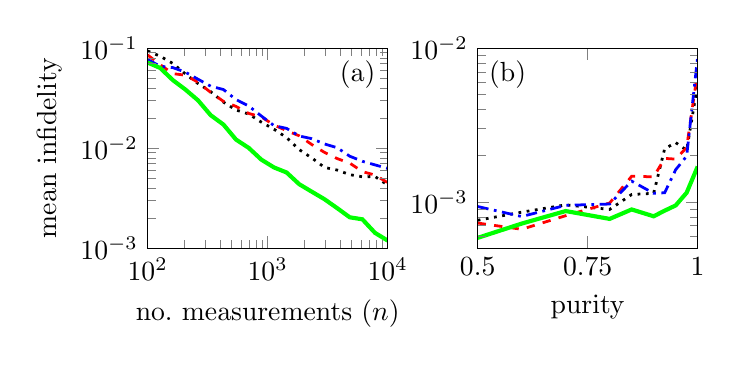
\begin{tikzpicture}

\begin{loglogaxis}[%
scale only axis,
width=1.2in,
height=1in,
xmin=100, xmax=10000,
ymin=0.001, ymax=0.1,
xlabel={no.\ measurements ($n$)},
ylabel={mean infidelity},
axis on top
,anchor=north west]
\addplot [
color=black,
dotted,
line width=1.0pt
]
coordinates{ (100,0.0936504) (127,0.0831784) (162,0.0703672) (206,0.0552666) (263,0.0442545) (335,0.0367459) (428,0.0288689) (545,0.0240754) (695,0.0219549) (885,0.0182243) (1128,0.0154802) (1438,0.0127685) (1832,0.00966868) (2335,0.00797919) (2976,0.00641328) (3792,0.00604222) (4832,0.00543209) (6158,0.0051745) (7847,0.0052069) (10000,0.00427943)
};
\label{leg:rand}

\addplot [
color=red,
dashed,
line width=1.0pt
]
coordinates{ (100,0.0854107) (127,0.0685189) (162,0.0556463) (206,0.0536513) (263,0.0455832) (335,0.0361215) (428,0.0293875) (545,0.0261447) (695,0.0222585) (885,0.0205318) (1128,0.0170572) (1438,0.0149583) (1832,0.0132948) (2335,0.0108542) (2976,0.00907246) (3792,0.00787257) (4832,0.0070859) (6158,0.00582692) (7847,0.00538335) (10000,0.00451835)
};

\addplot [
color=blue,
dash pattern=on 4pt off 2pt on 1pt off 2pt,
line width=1.0pt
]
coordinates{ (100,0.0770638) (127,0.066016) (162,0.0639258) (206,0.0575981) (263,0.0488788) (335,0.0416774) (428,0.0385588) (545,0.0306082) (695,0.0264267) (885,0.0209842) (1128,0.0168218) (1438,0.0157689) (1832,0.0132344) (2335,0.0124372) (2976,0.0110141) (3792,0.0101086) (4832,0.00830792) (6158,0.00739129) (7847,0.00680199) (10000,0.00627426)
};

\addplot [
color=green,
solid,
line width=1.5pt
]
coordinates{ (100,0.0717411) (127,0.0634239) (162,0.0479571) (206,0.0386032) (263,0.0300618) (335,0.0213717) (428,0.0172278) (545,0.0121796) (695,0.0100679) (885,0.00768467) (1128,0.0064199) (1438,0.00571155) (1832,0.00436206) (2335,0.00366658) (2976,0.0030864) (3792,0.0025154) (4832,0.00203493) (6158,0.00194272) (7847,0.00142223) (10000,0.00119099)
};
\label{leg:aFlex}

\end{loglogaxis}

% This file was created by matlab2tikz v0.0.7.
% Copyright (c) 2008--2010, Nico Schlömer <nico.schloemer@gmail.com>
% All rights reserved.
% 
% The latest updates can be retrieved from
%   http://www.mathworks.com/matlabcentral/fileexchange/22022-matlab2tikz
% where you can also make suggestions and rate matlab2tikz.
% 

\begin{semilogyaxis}[%
at={(1.65in,0)},
scale only axis,
width=1.1in,
height=1in,
xmin=0.5, xmax=1,
xtick={0.5,0.75,1},
ymin=0.0005, ymax=0.01,
xlabel={purity},
axis on top
,anchor=north west]
\addplot [
color=black,
dotted,
line width=1.0pt
]
coordinates{ (0.5,0.00075929) (0.6,0.000857054) (0.7,0.000956602) (0.8,0.000893443) (0.85,0.00111663) (0.9,0.00113761) (0.925,0.00221566) (0.95,0.0024295) (0.975,0.00216895) (1,0.00581406)
};


\addplot [
color=red,
dashed,
line width=1.0pt
]
coordinates{ (0.5,0.000728511) (0.6,0.000663376) (0.7,0.000813218) (0.8,0.000983281) (0.85,0.00146818) (0.9,0.00145583) (0.925,0.00191827) (0.95,0.00189825) (0.975,0.00225826) (1,0.00709776)
};

\addplot [
color=blue,
dash pattern=on 4pt off 2pt on 1pt off 2pt,
line width=1.0pt
]
coordinates{ (0.5,0.000933037) (0.6,0.000803118) (0.7,0.00094978) (0.8,0.000968539) (0.85,0.00136559) (0.9,0.00113676) (0.925,0.00114692) (0.95,0.0016187) (0.975,0.00198486) (1,0.00877819)
};

\addplot [
color=green,
solid,
line width=1.5pt
]
coordinates{ (0.5,0.000583439) (0.6,0.000722364) (0.7,0.000871828) (0.8,0.000775065) (0.85,0.000892919) (0.9,0.000805987) (0.925,0.00087682) (0.95,0.00094804) (0.975,0.00114797) (1,0.00169893)
};

\end{semilogyaxis}


\node at (1.05in,-0.13in) {(a)};
\node at (1.80in,-0.13in) {(b)};

\end{tikzpicture}

	\caption{One qubit tomography using projective measurements. \textbf{(a)}  Improvement of mean posterior fidelity as the experiment progresses. Results are shown for uniformly sampled measurements (\ref{leg:rand}), uniformly sampled Pauli measurements ( \ref{leg:MUB}), ABQT selecting adaptively amongst the 3 Pauli measurements (\ref{leg:aMUB}) and ABQT picking general measurements (\ref{leg:aFlex}). Adaptive optimisation of measurements allows for an almost $n^{-1}$ rate of convergence, while other methods are more consistent with a $n^{-\frac{1}{2}}$ rate. \textbf{(b)}  Final value of the mean posterior infidelity after 6000 measurements using the four methods as before, as a function of purity of the state to be estimated. The advantage of ABQT is greatest for purer states. \label{fig:qubit_results}}
\end{figure}

\begin{figure}[th]
	\resizebox{\columnwidth}{!}{
	% This file was created by matlab2tikz v0.0.7.
% Copyright (c) 2008--2010, Nico Schlömer <nico.schloemer@gmail.com>
% All rights reserved.
% 
% The latest updates can be retrieved from
%   http://www.mathworks.com/matlabcentral/fileexchange/22022-matlab2tikz
% where you can also make suggestions and rate matlab2tikz.
% 
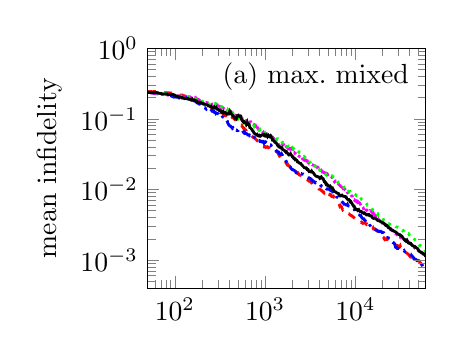
\begin{tikzpicture}

% defining custom colors
\definecolor{mycolor1}{rgb}{1,0,1}


\begin{loglogaxis}[%
scale only axis,
width= 1.39in,
height= 1.2in,
xmin=50, xmax=60000,
ymin=0.0004, ymax=1,
ylabel={mean infidelity},
axis on top]
\addplot [
color=red,
dashed,
line width=1.0pt
]
coordinates{ (50,0.242112) (51,0.242585) (52,0.242579) (52,0.242579) (53,0.24403) (53,0.24403) (54,0.243423) (55,0.243055) (55,0.243055) (56,0.241985) (56,0.241985) (57,0.242236) (58,0.242486) (58,0.242486) (59,0.242524) (60,0.242842) (60,0.242842) (61,0.243446) (62,0.243204) (62,0.243204) (63,0.244402) (64,0.246319) (64,0.246319) (65,0.244141) (66,0.244957) (67,0.245088) (67,0.245088) (68,0.242493) (69,0.24151) (70,0.241569) (70,0.241569) (71,0.240394) (72,0.239873) (73,0.237748) (74,0.236664) (74,0.236664) (75,0.234781) (76,0.234476) (77,0.233491) (78,0.233364) (79,0.234013) (80,0.234528) (80,0.234528) (81,0.232596) (82,0.233247) (83,0.23353) (84,0.233857) (85,0.233625) (86,0.233712) (87,0.231196) (88,0.232233) (89,0.231878) (90,0.229898) (91,0.231223) (92,0.232117) (93,0.23131) (94,0.231299) (95,0.231932) (96,0.232051) (97,0.232796) (98,0.232203) (99,0.230018) (100,0.230019) (102,0.226327) (103,0.224421) (104,0.225083) (105,0.224833) (106,0.22473) (107,0.221595) (109,0.220032) (110,0.219046) (111,0.217664) (112,0.217658) (113,0.216257) (115,0.214806) (116,0.216391) (117,0.215831) (119,0.21561) (120,0.216812) (121,0.214681) (123,0.213706) (124,0.211778) (125,0.212308) (127,0.212559) (128,0.212154) (130,0.20924) (131,0.208675) (132,0.206948) (134,0.205949) (135,0.204026) (137,0.201713) (138,0.20175) (140,0.199322) (142,0.197757) (143,0.19588) (145,0.194877) (146,0.195885) (148,0.197353) (150,0.19531) (151,0.196786) (153,0.194411) (155,0.192258) (156,0.192057) (158,0.191396) (160,0.192014) (162,0.189063) (163,0.188574) (165,0.188714) (167,0.186225) (169,0.185409) (171,0.183257) (173,0.182865) (175,0.181573) (177,0.181327) (178,0.179694) (180,0.180669) (182,0.178851) (184,0.176868) (187,0.17575) (189,0.174589) (191,0.174433) (193,0.173796) (195,0.174399) (197,0.177241) (199,0.176396) (202,0.171992) (204,0.171477) (206,0.169772) (208,0.168418) (211,0.166377) (213,0.16675) (215,0.166509) (218,0.164883) (220,0.163676) (223,0.162751) (225,0.16095) (228,0.160413) (230,0.160374) (233,0.158127) (235,0.155618) (238,0.154087) (240,0.153711) (243,0.152311) (246,0.150101) (249,0.148098) (251,0.146403) (254,0.148186) (257,0.145398) (260,0.143829) (263,0.143587) (266,0.138211) (268,0.139379) (271,0.141091) (274,0.137684) (278,0.13844) (281,0.139106) (284,0.136577) (287,0.136752) (290,0.134958) (293,0.133066) (297,0.131626) (300,0.130651) (303,0.130559) (306,0.129749) (310,0.129641) (313,0.129332) (317,0.129156) (320,0.128014) (324,0.127577) (327,0.123652) (331,0.122242) (335,0.122303) (338,0.120171) (342,0.117366) (346,0.117963) (350,0.116937) (354,0.115043) (358,0.112132) (362,0.110029) (366,0.11031) (370,0.112489) (374,0.110748) (378,0.110997) (382,0.113971) (386,0.113617) (391,0.113928) (395,0.113924) (399,0.112426) (404,0.109295) (408,0.104865) (413,0.107734) (417,0.108946) (422,0.108768) (427,0.106626) (431,0.108274) (436,0.106077) (441,0.105621) (446,0.105713) (451,0.100446) (456,0.0990345) (461,0.100679) (466,0.0993601) (471,0.0981938) (476,0.0974876) (482,0.0921608) (487,0.0911493) (492,0.0878769) (498,0.0881469) (503,0.0876396) (509,0.0842584) (515,0.0820276) (520,0.0818516) (526,0.0808978) (532,0.0802907) (538,0.0807572) (544,0.0799602) (550,0.080913) (556,0.0782933) (562,0.0769591) (568,0.0764293) (575,0.0737419) (581,0.0739429) (587,0.0732772) (594,0.0709154) (601,0.0704586) (607,0.0696448) (614,0.0691798) (621,0.0664823) (628,0.0663546) (635,0.0658588) (642,0.0661367) (649,0.0652651) (656,0.0639388) (663,0.0643139) (670,0.0636474) (678,0.0624409) (685,0.0625673) (693,0.0610222) (701,0.0593282) (708,0.0574196) (716,0.0570385) (724,0.055619) (732,0.0551673) (740,0.0543723) (749,0.0541598) (757,0.0534892) (765,0.0535717) (774,0.0525225) (782,0.0516469) (791,0.0510018) (800,0.0504779) (809,0.0496023) (818,0.0491597) (827,0.0484678) (836,0.0483383) (845,0.04814) (854,0.0473097) (864,0.0467625) (873,0.0462294) (883,0.04573) (893,0.0459103) (903,0.0463183) (913,0.0454748) (923,0.0448473) (933,0.044251) (944,0.0421132) (954,0.0409368) (965,0.0409889) (975,0.0401149) (986,0.0403282) (997,0.0399024) (1008,0.0400981) (1019,0.039474) (1030,0.0399374) (1042,0.0400972) (1053,0.0397222) (1065,0.0400951) (1077,0.0397076) (1089,0.0395973) (1101,0.0386093) (1113,0.0384593) (1125,0.0375175) (1138,0.0369009) (1151,0.0364406) (1163,0.0370622) (1176,0.0363621) (1189,0.036502) (1202,0.0362867) (1216,0.0361759) (1229,0.036435) (1243,0.035918) (1257,0.0364149) (1270,0.0360599) (1285,0.0364668) (1299,0.0355528) (1313,0.0348065) (1328,0.03435) (1342,0.0341536) (1357,0.034145) (1372,0.03336) (1387,0.0327012) (1403,0.0318691) (1418,0.0309205) (1434,0.0300299) (1450,0.0293274) (1466,0.0284043) (1482,0.0275779) (1499,0.0269067) (1515,0.0265167) (1532,0.0266147) (1549,0.0260765) (1566,0.0255448) (1584,0.0258892) (1601,0.0257621) (1619,0.0255801) (1637,0.0259807) (1655,0.025697) (1673,0.0253994) (1692,0.024382) (1711,0.023568) (1730,0.0230014) (1749,0.0225454) (1768,0.0229644) (1788,0.0223319) (1807,0.0219216) (1827,0.0217694) (1848,0.0213455) (1868,0.0212474) (1889,0.0212692) (1910,0.0209884) (1931,0.0208423) (1952,0.0205148) (1974,0.0205279) (1996,0.0203834) (2018,0.0203135) (2040,0.0204835) (2063,0.0205762) (2086,0.0198646) (2109,0.0197941) (2132,0.0193017) (2156,0.0185179) (2180,0.0181675) (2204,0.0179048) (2228,0.0175866) (2253,0.0174143) (2278,0.0168682) (2303,0.016823) (2329,0.0169768) (2354,0.0165241) (2380,0.0160877) (2407,0.015946) (2433,0.0158434) (2460,0.0158037) (2488,0.0159035) (2515,0.0153528) (2543,0.0152888) (2571,0.014656) (2600,0.0144204) (2629,0.0144689) (2658,0.0144305) (2687,0.0143074) (2717,0.0141892) (2747,0.0141485) (2777,0.0141188) (2808,0.0141874) (2839,0.013948) (2871,0.0141196) (2902,0.0140519) (2935,0.0138061) (2967,0.0138598) (3000,0.0134693) (3033,0.0132234) (3067,0.0133144) (3101,0.0134289) (3135,0.0130241) (3170,0.0129789) (3205,0.0126841) (3240,0.0126093) (3276,0.01233) (3313,0.0121895) (3349,0.0119393) (3386,0.0119509) (3424,0.0117246) (3462,0.0115072) (3500,0.0114163) (3539,0.011465) (3578,0.0113329) (3618,0.0113103) (3658,0.011058) (3698,0.0108744) (3739,0.0108468) (3781,0.0108409) (3823,0.010641) (3865,0.0105088) (3908,0.0103946) (3951,0.0100973) (3995,0.0100948) (4039,0.0100368) (4084,0.0100342) (4129,0.00987675) (4175,0.00974444) (4221,0.00957576) (4268,0.00957283) (4315,0.00936276) (4363,0.00930829) (4411,0.009125) (4460,0.00917423) (4509,0.00897195) (4559,0.00918345) (4610,0.00881692) (4661,0.00862951) (4712,0.00845777) (4765,0.00838558) (4817,0.00849491) (4871,0.00836588) (4925,0.00830536) (4979,0.00856845) (5034,0.0087088) (5090,0.00877004) (5147,0.00848654) (5204,0.00856098) (5261,0.00853308) (5319,0.00844609) (5378,0.00806394) (5438,0.00798653) (5498,0.00803056) (5559,0.00795477) (5621,0.00807503) (5683,0.0081) (5746,0.00780881) (5809,0.00771761) (5874,0.0076491) (5939,0.00760529) (6005,0.00759336) (6071,0.00741446) (6138,0.00718706) (6206,0.00695547) (6275,0.00688713) (6345,0.00674647) (6415,0.00642484) (6486,0.00639219) (6558,0.00630032) (6630,0.00605567) (6704,0.00582944) (6778,0.00595932) (6853,0.00585274) (6929,0.00576531) (7006,0.00571136) (7083,0.00546021) (7162,0.00530161) (7241,0.00515857) (7321,0.00523902) (7402,0.00528926) (7484,0.00523296) (7567,0.00521496) (7651,0.0052585) (7736,0.00523116) (7821,0.00515706) (7908,0.00502496) (7996,0.00496738) (8084,0.00491259) (8174,0.00481533) (8264,0.004622) (8356,0.00455445) (8448,0.00453907) (8542,0.00448746) (8636,0.00441189) (8732,0.00436698) (8829,0.00431797) (8926,0.00426717) (9025,0.0042637) (9125,0.00425269) (9226,0.00419374) (9329,0.00409975) (9432,0.00405875) (9536,0.00406442) (9642,0.00400221) (9749,0.00392948) (9857,0.00387923) (9966,0.00388355) (10076,0.00391615) (10188,0.0038688) (10301,0.00377706) (10415,0.0036485) (10530,0.00359019) (10647,0.00354625) (10764,0.00346061) (10884,0.00342241) (11004,0.00340341) (11126,0.00343161) (11249,0.003402) (11374,0.00340904) (11500,0.00342741) (11627,0.00339936) (11756,0.00345482) (11886,0.0034291) (12018,0.00336167) (12151,0.00330788) (12285,0.00331126) (12422,0.00334207) (12559,0.00334683) (12698,0.00334884) (12839,0.00335387) (12981,0.00329542) (13125,0.00322448) (13270,0.00318388) (13417,0.003213) (13566,0.00314166) (13716,0.00306387) (13868,0.00299366) (14021,0.00297537) (14177,0.00297918) (14334,0.0029811) (14492,0.00298991) (14653,0.00290419) (14815,0.00283768) (14979,0.00280477) (15145,0.00284513) (15313,0.00284816) (15482,0.00281885) (15654,0.00286242) (15827,0.00275265) (16002,0.00273214) (16180,0.00273461) (16359,0.00276487) (16540,0.00270588) (16723,0.00266552) (16908,0.00264213) (17096,0.00265933) (17285,0.0026067) (17476,0.00258606) (17670,0.0025325) (17866,0.00241869) (18063,0.00234081) (18263,0.00230054) (18466,0.00227951) (18670,0.00232174) (18877,0.00231254) (19086,0.00229633) (19297,0.00226231) (19511,0.00226605) (19727,0.00224609) (19946,0.00221274) (20166,0.00213161) (20390,0.00210707) (20616,0.00207241) (20844,0.00200996) (21075,0.00196253) (21308,0.0019911) (21544,0.00199727) (21783,0.0020038) (22024,0.00194626) (22268,0.00195146) (22514,0.00194985) (22764,0.00198226) (23016,0.00196917) (23271,0.00194878) (23528,0.00190125) (23789,0.00189583) (24052,0.00188273) (24319,0.00185027) (24588,0.00182749) (24860,0.00183966) (25136,0.00182481) (25414,0.00180968) (25695,0.00179346) (25980,0.00178872) (26268,0.00176881) (26559,0.00170389) (26853,0.00166862) (27150,0.00167181) (27451,0.00165901) (27755,0.00163068) (28062,0.00162982) (28373,0.00163265) (28687,0.00161975) (29005,0.001611) (29326,0.00159812) (29651,0.00156741) (29979,0.00155328) (30311,0.00156968) (30647,0.00155023) (30986,0.00153895) (31329,0.00157963) (31676,0.00150433) (32027,0.00148119) (32382,0.00144136) (32740,0.00141001) (33103,0.00141559) (33470,0.00138226) (33840,0.00138394) (34215,0.00137697) (34594,0.00138307) (34977,0.00135618) (35364,0.00133589) (35756,0.00131473) (36152,0.00131601) (36552,0.00126535) (36957,0.00125773) (37366,0.00124385) (37780,0.00123247) (38198,0.00120755) (38621,0.00120162) (39049,0.00118866) (39482,0.00115987) (39919,0.00113952) (40361,0.00113351) (40808,0.00110385) (41260,0.00109537) (41717,0.00109059) (42179,0.00108983) (42646,0.00106938) (43118,0.00105283) (43595,0.00103544) (44078,0.00103498) (44566,0.00101354) (45060,0.00100789) (45559,0.000988695) (46063,0.000976631) (46574,0.000965344) (47089,0.000973902) (47611,0.000993019) (48138,0.000989589) (48671,0.00100712) (49210,0.000994455) (49755,0.000980015) (50306,0.000987018) (50863,0.000979309) (51426,0.000943314) (51996,0.000929992) (52572,0.000902347) (53154,0.00089843) (53743,0.000881914) (54338,0.00086914) (54939,0.000851085) (55548,0.000835695) (56163,0.000825863) (56785,0.000824847) (57414,0.000816275) (58050,0.000805981) (58692,0.000803881) (59342,0.000796648) (60000,0.000776451)
};
\label{leg:MUB}

\addplot [
color=mycolor1,
dash pattern=on 4pt off 1pt on 1pt off 1pt on 1pt off 1pt,
line width=1.0pt
]
coordinates{ (50,0.23596) (51,0.235546) (52,0.235875) (52,0.235875) (53,0.234363) (53,0.234363) (54,0.233442) (55,0.231968) (55,0.231968) (56,0.231899) (56,0.231899) (57,0.233148) (58,0.230209) (58,0.230209) (59,0.228557) (60,0.227576) (60,0.227576) (61,0.226536) (62,0.226344) (62,0.226344) (63,0.226271) (64,0.22497) (64,0.22497) (65,0.224669) (66,0.224387) (67,0.224531) (67,0.224531) (68,0.224225) (69,0.222678) (70,0.222929) (70,0.222929) (71,0.222079) (72,0.220077) (73,0.220892) (74,0.220586) (74,0.220586) (75,0.220904) (76,0.218739) (77,0.218358) (78,0.217974) (79,0.218795) (80,0.217648) (80,0.217648) (81,0.218702) (82,0.218166) (83,0.216361) (84,0.216213) (85,0.21656) (86,0.215523) (87,0.21398) (88,0.213157) (89,0.213475) (90,0.212095) (91,0.212331) (92,0.212808) (93,0.211846) (94,0.212082) (95,0.211861) (96,0.210499) (97,0.209933) (98,0.209969) (99,0.209091) (100,0.209638) (102,0.209244) (103,0.20711) (104,0.208269) (105,0.208726) (106,0.209568) (107,0.20914) (109,0.210753) (110,0.211949) (111,0.211301) (112,0.211425) (113,0.211831) (115,0.208568) (116,0.207978) (117,0.207083) (119,0.209551) (120,0.20989) (121,0.20842) (123,0.210324) (124,0.207744) (125,0.207208) (127,0.206769) (128,0.207847) (130,0.204948) (131,0.205509) (132,0.204419) (134,0.202774) (135,0.201146) (137,0.200894) (138,0.202511) (140,0.200238) (142,0.201034) (143,0.200766) (145,0.198618) (146,0.198895) (148,0.198163) (150,0.199221) (151,0.20068) (153,0.198829) (155,0.196401) (156,0.196084) (158,0.195973) (160,0.196432) (162,0.19584) (163,0.195376) (165,0.197066) (167,0.198105) (169,0.200205) (171,0.196314) (173,0.19322) (175,0.192301) (177,0.191425) (178,0.188465) (180,0.189082) (182,0.187876) (184,0.186984) (187,0.182678) (189,0.179757) (191,0.179604) (193,0.177237) (195,0.174954) (197,0.173137) (199,0.174319) (202,0.17237) (204,0.17147) (206,0.169894) (208,0.171501) (211,0.172184) (213,0.171825) (215,0.171084) (218,0.170825) (220,0.169285) (223,0.170123) (225,0.167946) (228,0.16724) (230,0.166966) (233,0.168138) (235,0.167149) (238,0.166757) (240,0.167245) (243,0.165331) (246,0.161942) (249,0.161527) (251,0.160767) (254,0.160725) (257,0.159786) (260,0.16221) (263,0.162105) (266,0.161921) (268,0.161846) (271,0.160369) (274,0.158719) (278,0.157119) (281,0.15696) (284,0.158724) (287,0.15996) (290,0.160041) (293,0.15942) (297,0.153403) (300,0.153379) (303,0.150971) (306,0.150982) (310,0.150935) (313,0.149652) (317,0.14801) (320,0.14571) (324,0.144911) (327,0.143767) (331,0.144345) (335,0.144266) (338,0.143796) (342,0.141889) (346,0.140959) (350,0.138666) (354,0.137074) (358,0.136116) (362,0.134211) (366,0.130989) (370,0.13112) (374,0.128256) (378,0.129208) (382,0.128776) (386,0.129445) (391,0.127197) (395,0.130252) (399,0.131218) (404,0.130184) (408,0.129146) (413,0.127661) (417,0.126115) (422,0.125797) (427,0.122412) (431,0.122286) (436,0.11933) (441,0.118052) (446,0.115524) (451,0.116064) (456,0.115397) (461,0.11355) (466,0.112374) (471,0.111639) (476,0.110704) (482,0.111281) (487,0.110465) (492,0.110231) (498,0.110366) (503,0.109975) (509,0.110995) (515,0.107136) (520,0.103887) (526,0.103356) (532,0.101799) (538,0.101952) (544,0.101865) (550,0.101586) (556,0.101664) (562,0.0998702) (568,0.0992549) (575,0.0982313) (581,0.0982131) (587,0.0981454) (594,0.0958616) (601,0.0948175) (607,0.0943465) (614,0.0945541) (621,0.0947448) (628,0.0925748) (635,0.093622) (642,0.0944261) (649,0.0938145) (656,0.0934678) (663,0.0903747) (670,0.0887216) (678,0.0896727) (685,0.0905785) (693,0.0906841) (701,0.0876833) (708,0.0865613) (716,0.0868769) (724,0.0853184) (732,0.0850275) (740,0.0844432) (749,0.0839944) (757,0.081139) (765,0.0811305) (774,0.0800049) (782,0.0805929) (791,0.0780291) (800,0.0768111) (809,0.0762692) (818,0.0758689) (827,0.0737726) (836,0.0723827) (845,0.0710108) (854,0.0695616) (864,0.0687406) (873,0.0683103) (883,0.0662622) (893,0.0649621) (903,0.062952) (913,0.062627) (923,0.061827) (933,0.0622969) (944,0.0637959) (954,0.064556) (965,0.0624381) (975,0.0614655) (986,0.0631099) (997,0.0628238) (1008,0.0621894) (1019,0.0615608) (1030,0.0618135) (1042,0.0615834) (1053,0.061037) (1065,0.0605649) (1077,0.0601939) (1089,0.059521) (1101,0.0584729) (1113,0.0575333) (1125,0.0563717) (1138,0.056805) (1151,0.056969) (1163,0.0563021) (1176,0.0557726) (1189,0.0544225) (1202,0.0546514) (1216,0.0546622) (1229,0.0531219) (1243,0.052868) (1257,0.0503834) (1270,0.0493533) (1285,0.0494298) (1299,0.0489588) (1313,0.04766) (1328,0.0458325) (1342,0.0449984) (1357,0.0451219) (1372,0.0436401) (1387,0.0442231) (1403,0.0437613) (1418,0.0429277) (1434,0.0422618) (1450,0.0426467) (1466,0.0430995) (1482,0.0434977) (1499,0.0423506) (1515,0.0418411) (1532,0.0426671) (1549,0.0429823) (1566,0.0426471) (1584,0.0425787) (1601,0.0429761) (1619,0.0418639) (1637,0.042614) (1655,0.0421099) (1673,0.0423704) (1692,0.0424008) (1711,0.0405635) (1730,0.0402651) (1749,0.0395978) (1768,0.0390183) (1788,0.0387662) (1807,0.0378214) (1827,0.0380544) (1848,0.0375341) (1868,0.0378116) (1889,0.0372633) (1910,0.0378586) (1931,0.038097) (1952,0.0383371) (1974,0.03746) (1996,0.0367997) (2018,0.0364951) (2040,0.0350381) (2063,0.0331747) (2086,0.0325865) (2109,0.0329989) (2132,0.0323824) (2156,0.0325818) (2180,0.0320478) (2204,0.0314599) (2228,0.0305261) (2253,0.0303578) (2278,0.0301295) (2303,0.0300973) (2329,0.0298342) (2354,0.0296323) (2380,0.029635) (2407,0.0291515) (2433,0.0288893) (2460,0.0286282) (2488,0.0282631) (2515,0.0288183) (2543,0.0285424) (2571,0.0279642) (2600,0.0270572) (2629,0.0268527) (2658,0.0267538) (2687,0.0261437) (2717,0.0258853) (2747,0.0257881) (2777,0.0255556) (2808,0.0256364) (2839,0.0259783) (2871,0.025694) (2902,0.0252367) (2935,0.0252962) (2967,0.0247793) (3000,0.0242199) (3033,0.02367) (3067,0.0232569) (3101,0.0228569) (3135,0.0227321) (3170,0.0225536) (3205,0.0227917) (3240,0.0227211) (3276,0.0226437) (3313,0.0223251) (3349,0.0223656) (3386,0.0220928) (3424,0.0219892) (3462,0.0218333) (3500,0.0214684) (3539,0.0213539) (3578,0.021209) (3618,0.0211448) (3658,0.0213774) (3698,0.0211698) (3739,0.020667) (3781,0.0207764) (3823,0.0206732) (3865,0.0202941) (3908,0.019714) (3951,0.0196463) (3995,0.0193064) (4039,0.0190029) (4084,0.0186178) (4129,0.0186104) (4175,0.0187585) (4221,0.0183339) (4268,0.0181296) (4315,0.017654) (4363,0.0177664) (4411,0.0175958) (4460,0.0173542) (4509,0.0171618) (4559,0.0172723) (4610,0.0170608) (4661,0.0171096) (4712,0.0170541) (4765,0.016987) (4817,0.0168539) (4871,0.016607) (4925,0.0162898) (4979,0.0161315) (5034,0.0160779) (5090,0.0160695) (5147,0.0156715) (5204,0.0155864) (5261,0.0155718) (5319,0.0155267) (5378,0.0153995) (5438,0.0152128) (5498,0.014705) (5559,0.0145351) (5621,0.0142207) (5683,0.0139027) (5746,0.0135167) (5809,0.0131402) (5874,0.0128237) (5939,0.0129981) (6005,0.0131547) (6071,0.0130366) (6138,0.0128059) (6206,0.0125946) (6275,0.0124639) (6345,0.0122407) (6415,0.0122681) (6486,0.0120041) (6558,0.011702) (6630,0.0115648) (6704,0.0114808) (6778,0.0113187) (6853,0.0110737) (6929,0.0109033) (7006,0.0108717) (7083,0.0107985) (7162,0.0106857) (7241,0.0105054) (7321,0.0102616) (7402,0.0103352) (7484,0.0102402) (7567,0.0100899) (7651,0.0099658) (7736,0.00991195) (7821,0.00963213) (7908,0.0096735) (7996,0.00951845) (8084,0.00911133) (8174,0.00903158) (8264,0.00887706) (8356,0.00886647) (8448,0.00868879) (8542,0.0086259) (8636,0.00849033) (8732,0.0083731) (8829,0.00832492) (8926,0.00836411) (9025,0.00818021) (9125,0.00807715) (9226,0.00801176) (9329,0.00775786) (9432,0.0074459) (9536,0.00724555) (9642,0.00721865) (9749,0.00714172) (9857,0.00691462) (9966,0.00690932) (10076,0.00678832) (10188,0.00677207) (10301,0.00685338) (10415,0.00673385) (10530,0.00659034) (10647,0.00669864) (10764,0.00655633) (10884,0.00657518) (11004,0.00650413) (11126,0.00644414) (11249,0.00630601) (11374,0.00612743) (11500,0.00593275) (11627,0.00583129) (11756,0.00582886) (11886,0.00572623) (12018,0.00568106) (12151,0.00559491) (12285,0.0053502) (12422,0.0053459) (12559,0.00550741) (12698,0.00531815) (12839,0.00529153) (12981,0.00531371) (13125,0.00518358) (13270,0.00515683) (13417,0.00510145) (13566,0.00493582) (13716,0.00489902) (13868,0.00485178) (14021,0.00483856) (14177,0.004882) (14334,0.00494352) (14492,0.00500471) (14653,0.00498453) (14815,0.00492928) (14979,0.00492885) (15145,0.00483987) (15313,0.00486616) (15482,0.00462853) (15654,0.00456632) (15827,0.0046198) (16002,0.00453894) (16180,0.004416) (16359,0.00433445) (16540,0.00422043) (16723,0.00419873) (16908,0.0040953) (17096,0.00411866) (17285,0.00405214) (17476,0.00384542) (17670,0.00380489) (17866,0.00383169) (18063,0.0037689) (18263,0.00372569) (18466,0.00364675) (18670,0.00364127) (18877,0.00363312) (19086,0.00362421) (19297,0.00354932) (19511,0.00350541) (19727,0.00352714) (19946,0.00349437) (20166,0.00339798) (20390,0.00336826) (20616,0.00331003) (20844,0.0032978) (21075,0.00327269) (21308,0.00327786) (21544,0.00325939) (21783,0.0031814) (22024,0.00309065) (22268,0.00307687) (22514,0.00301797) (22764,0.00301549) (23016,0.00295767) (23271,0.0028652) (23528,0.00286972) (23789,0.0028166) (24052,0.00279325) (24319,0.00270781) (24588,0.0026828) (24860,0.00272588) (25136,0.00269507) (25414,0.00263604) (25695,0.00260982) (25980,0.00258092) (26268,0.00256462) (26559,0.00252644) (26853,0.00249484) (27150,0.00244831) (27451,0.00243838) (27755,0.00238238) (28062,0.00236097) (28373,0.00235348) (28687,0.00229123) (29005,0.00226364) (29326,0.00226227) (29651,0.00222901) (29979,0.00221804) (30311,0.0021948) (30647,0.00218624) (30986,0.00218228) (31329,0.00215774) (31676,0.00207168) (32027,0.00206252) (32382,0.00204457) (32740,0.00205398) (33103,0.00200774) (33470,0.00198399) (33840,0.0019827) (34215,0.0019747) (34594,0.00194385) (34977,0.00194988) (35364,0.00195383) (35756,0.0019347) (36152,0.00191321) (36552,0.00189008) (36957,0.00183943) (37366,0.0018342) (37780,0.0018444) (38198,0.00183472) (38621,0.00180049) (39049,0.00176501) (39482,0.00175115) (39919,0.00173355) (40361,0.0017148) (40808,0.00168901) (41260,0.00168287) (41717,0.00166922) (42179,0.00165122) (42646,0.00162578) (43118,0.0015849) (43595,0.00159641) (44078,0.00155569) (44566,0.00152811) (45060,0.00150522) (45559,0.00147198) (46063,0.00144375) (46574,0.00141829) (47089,0.00138591) (47611,0.00137043) (48138,0.00139949) (48671,0.00139972) (49210,0.00138755) (49755,0.00140963) (50306,0.00138572) (50863,0.00136685) (51426,0.00136841) (51996,0.00130237) (52572,0.00129097) (53154,0.00127771) (53743,0.00128813) (54338,0.00127001) (54939,0.00125493) (55548,0.00124767) (56163,0.00122487) (56785,0.00120326) (57414,0.00119592) (58050,0.0011947) (58692,0.00117596) (59342,0.00116105) (60000,0.00116016)
};
\label{leg:SSQT}


\addplot [
color=blue,
dash pattern=on 4pt off 2pt on 1pt off 2pt,
line width=1.0pt
]
coordinates{ (50,0.236692) (51,0.236518) (52,0.235451) (52,0.235451) (53,0.236699) (53,0.236699) (54,0.236188) (55,0.235942) (55,0.235942) (56,0.233796) (56,0.233796) (57,0.23273) (58,0.234419) (58,0.234419) (59,0.234006) (60,0.235358) (60,0.235358) (61,0.236169) (62,0.23476) (62,0.23476) (63,0.233434) (64,0.233874) (64,0.233874) (65,0.234605) (66,0.234046) (67,0.234207) (67,0.234207) (68,0.231319) (69,0.23296) (70,0.232434) (70,0.232434) (71,0.232586) (72,0.232575) (73,0.232357) (74,0.229941) (74,0.229941) (75,0.229918) (76,0.229402) (77,0.227299) (78,0.226133) (79,0.228312) (80,0.223723) (80,0.223723) (81,0.222972) (82,0.22421) (83,0.219658) (84,0.218898) (85,0.221227) (86,0.220509) (87,0.21862) (88,0.220013) (89,0.219314) (90,0.217371) (91,0.212271) (92,0.208456) (93,0.208008) (94,0.207286) (95,0.205173) (96,0.204503) (97,0.204103) (98,0.202546) (99,0.202813) (100,0.204135) (102,0.205127) (103,0.204675) (104,0.201953) (105,0.201373) (106,0.20184) (107,0.202801) (109,0.201047) (110,0.199902) (111,0.199452) (112,0.196684) (113,0.197828) (115,0.197678) (116,0.197597) (117,0.198512) (119,0.197987) (120,0.197051) (121,0.195765) (123,0.197215) (124,0.196228) (125,0.195966) (127,0.196889) (128,0.195822) (130,0.196281) (131,0.19795) (132,0.195719) (134,0.197454) (135,0.19839) (137,0.19262) (138,0.191619) (140,0.19233) (142,0.185978) (143,0.186148) (145,0.187943) (146,0.187381) (148,0.187489) (150,0.184195) (151,0.184359) (153,0.184001) (155,0.185608) (156,0.185954) (158,0.182238) (160,0.181933) (162,0.180073) (163,0.17995) (165,0.178626) (167,0.177355) (169,0.177759) (171,0.17857) (173,0.172423) (175,0.169223) (177,0.170109) (178,0.169535) (180,0.166867) (182,0.165423) (184,0.162306) (187,0.160962) (189,0.162394) (191,0.160766) (193,0.160341) (195,0.157771) (197,0.155312) (199,0.152989) (202,0.151942) (204,0.149235) (206,0.148698) (208,0.145881) (211,0.143906) (213,0.143251) (215,0.143894) (218,0.141125) (220,0.138625) (223,0.136677) (225,0.138602) (228,0.140984) (230,0.140531) (233,0.140471) (235,0.13745) (238,0.135895) (240,0.137908) (243,0.140447) (246,0.139182) (249,0.136788) (251,0.134522) (254,0.132203) (257,0.130568) (260,0.127443) (263,0.127449) (266,0.126372) (268,0.126001) (271,0.124655) (274,0.126402) (278,0.12389) (281,0.122604) (284,0.119421) (287,0.121448) (290,0.120861) (293,0.120089) (297,0.119204) (300,0.11789) (303,0.117867) (306,0.114335) (310,0.111692) (313,0.109662) (317,0.10832) (320,0.107438) (324,0.111316) (327,0.111474) (331,0.112468) (335,0.108851) (338,0.106482) (342,0.105476) (346,0.105134) (350,0.104301) (354,0.10348) (358,0.101697) (362,0.101611) (366,0.09846) (370,0.0968029) (374,0.0979335) (378,0.0933225) (382,0.0925224) (386,0.0867117) (391,0.0848351) (395,0.0825293) (399,0.0809308) (404,0.0798966) (408,0.0788583) (413,0.0788547) (417,0.0777665) (422,0.0769953) (427,0.0750852) (431,0.0753419) (436,0.0729614) (441,0.0738141) (446,0.0706499) (451,0.0714645) (456,0.0714936) (461,0.0726573) (466,0.0728765) (471,0.0706888) (476,0.0689184) (482,0.0692326) (487,0.0680991) (492,0.0677571) (498,0.0679386) (503,0.0681494) (509,0.0702839) (515,0.0716949) (520,0.0698127) (526,0.0698213) (532,0.0691321) (538,0.0685537) (544,0.0689843) (550,0.0688634) (556,0.0680671) (562,0.0672541) (568,0.0655337) (575,0.0644867) (581,0.0648933) (587,0.0632778) (594,0.0640682) (601,0.0621407) (607,0.062229) (614,0.0616665) (621,0.0617754) (628,0.0615597) (635,0.0603757) (642,0.0591095) (649,0.0591579) (656,0.0588735) (663,0.0591029) (670,0.0579302) (678,0.0587389) (685,0.0582961) (693,0.0592705) (701,0.0577602) (708,0.0582272) (716,0.0586564) (724,0.0600195) (732,0.0587491) (740,0.0579008) (749,0.0561564) (757,0.0546704) (765,0.0542702) (774,0.0525588) (782,0.0519872) (791,0.0519896) (800,0.0503886) (809,0.0493911) (818,0.0494748) (827,0.0492821) (836,0.04897) (845,0.04935) (854,0.0481943) (864,0.0487205) (873,0.0478225) (883,0.0477735) (893,0.0484747) (903,0.0481833) (913,0.0471933) (923,0.0469066) (933,0.0477421) (944,0.0479392) (954,0.0471183) (965,0.0464901) (975,0.0451943) (986,0.0461726) (997,0.0461598) (1008,0.047312) (1019,0.0470608) (1030,0.0461291) (1042,0.0455622) (1053,0.044195) (1065,0.0436237) (1077,0.0429524) (1089,0.0436113) (1101,0.0439319) (1113,0.0426509) (1125,0.0430017) (1138,0.0429655) (1151,0.0429461) (1163,0.0425076) (1176,0.0409508) (1189,0.040194) (1202,0.0400948) (1216,0.0400147) (1229,0.0396025) (1243,0.0396457) (1257,0.0392811) (1270,0.0384218) (1285,0.0379422) (1299,0.0377528) (1313,0.0366674) (1328,0.0356864) (1342,0.0353849) (1357,0.0346878) (1372,0.0345219) (1387,0.0334615) (1403,0.0333755) (1418,0.0334476) (1434,0.0321163) (1450,0.0316485) (1466,0.0313852) (1482,0.0316076) (1499,0.0317042) (1515,0.0321559) (1532,0.0311487) (1549,0.0308167) (1566,0.0297266) (1584,0.0291811) (1601,0.0286266) (1619,0.0273361) (1637,0.0265224) (1655,0.0264716) (1673,0.0261489) (1692,0.0253369) (1711,0.0251368) (1730,0.0242292) (1749,0.0239988) (1768,0.0236082) (1788,0.0228232) (1807,0.022008) (1827,0.0220045) (1848,0.0209557) (1868,0.0209926) (1889,0.0206127) (1910,0.020608) (1931,0.0199206) (1952,0.0195565) (1974,0.0194349) (1996,0.0190966) (2018,0.0191502) (2040,0.0188591) (2063,0.0188694) (2086,0.0187203) (2109,0.0185544) (2132,0.0182332) (2156,0.0180458) (2180,0.0177582) (2204,0.0171739) (2228,0.0171799) (2253,0.0171372) (2278,0.0171299) (2303,0.0171716) (2329,0.0175293) (2354,0.0179208) (2380,0.0181241) (2407,0.0175688) (2433,0.0174474) (2460,0.0171999) (2488,0.0167866) (2515,0.0167698) (2543,0.0165424) (2571,0.0165223) (2600,0.0164667) (2629,0.0165133) (2658,0.0164627) (2687,0.0163033) (2717,0.0162632) (2747,0.0161651) (2777,0.0160435) (2808,0.0157518) (2839,0.0154943) (2871,0.0150875) (2902,0.0148769) (2935,0.0147503) (2967,0.0146853) (3000,0.0146712) (3033,0.0145825) (3067,0.014599) (3101,0.0143571) (3135,0.0142899) (3170,0.0142809) (3205,0.014099) (3240,0.0140213) (3276,0.013558) (3313,0.013565) (3349,0.0134066) (3386,0.0130235) (3424,0.0130302) (3462,0.0129636) (3500,0.0128505) (3539,0.0125807) (3578,0.012441) (3618,0.0126498) (3658,0.0125952) (3698,0.0124041) (3739,0.0122046) (3781,0.0122557) (3823,0.0121388) (3865,0.0120111) (3908,0.0119485) (3951,0.0119434) (3995,0.0119422) (4039,0.011886) (4084,0.0117222) (4129,0.0113541) (4175,0.0113684) (4221,0.0110329) (4268,0.0108795) (4315,0.0107775) (4363,0.010425) (4411,0.0103003) (4460,0.0104114) (4509,0.0104782) (4559,0.010485) (4610,0.010251) (4661,0.0103893) (4712,0.0102563) (4765,0.0101903) (4817,0.0100969) (4871,0.0101793) (4925,0.0100653) (4979,0.0100771) (5034,0.0100425) (5090,0.0101043) (5147,0.00992923) (5204,0.00979321) (5261,0.00971432) (5319,0.00963943) (5378,0.00989938) (5438,0.00988153) (5498,0.00978464) (5559,0.00970038) (5621,0.00912397) (5683,0.00888788) (5746,0.00847518) (5809,0.00836916) (5874,0.00855477) (5939,0.00856716) (6005,0.00840954) (6071,0.00820815) (6138,0.00798756) (6206,0.00777821) (6275,0.00774609) (6345,0.00776223) (6415,0.00778138) (6486,0.00757979) (6558,0.00740666) (6630,0.00730413) (6704,0.00715727) (6778,0.00708302) (6853,0.00705714) (6929,0.00693823) (7006,0.0068948) (7083,0.00671518) (7162,0.00666464) (7241,0.00646429) (7321,0.00647637) (7402,0.00634496) (7484,0.00618648) (7567,0.00618336) (7651,0.00615534) (7736,0.00612537) (7821,0.00606303) (7908,0.00601338) (7996,0.00604363) (8084,0.00599514) (8174,0.00613932) (8264,0.0059248) (8356,0.0059043) (8448,0.00580793) (8542,0.00577599) (8636,0.00576181) (8732,0.00571418) (8829,0.00565835) (8926,0.00554071) (9025,0.00549571) (9125,0.00548131) (9226,0.00528833) (9329,0.00536174) (9432,0.0053124) (9536,0.00528283) (9642,0.00521516) (9749,0.00512662) (9857,0.00510578) (9966,0.00492873) (10076,0.00474695) (10188,0.00461306) (10301,0.00453084) (10415,0.00447376) (10530,0.00442415) (10647,0.00443146) (10764,0.00438678) (10884,0.00438361) (11004,0.00434479) (11126,0.00434035) (11249,0.00427249) (11374,0.00421447) (11500,0.00423475) (11627,0.00411869) (11756,0.00399187) (11886,0.00393847) (12018,0.00388661) (12151,0.00386109) (12285,0.00382069) (12422,0.00382617) (12559,0.0037269) (12698,0.00369296) (12839,0.00363975) (12981,0.00353791) (13125,0.0034381) (13270,0.00350783) (13417,0.00352399) (13566,0.00344826) (13716,0.00339873) (13868,0.00333269) (14021,0.00331871) (14177,0.00327382) (14334,0.00316607) (14492,0.00310211) (14653,0.0030561) (14815,0.00297759) (14979,0.00293195) (15145,0.00286682) (15313,0.00283365) (15482,0.00277108) (15654,0.0027668) (15827,0.00279222) (16002,0.00277165) (16180,0.00277735) (16359,0.00274054) (16540,0.0027114) (16723,0.00270198) (16908,0.00267892) (17096,0.00264878) (17285,0.00264229) (17476,0.00259457) (17670,0.00257267) (17866,0.00255094) (18063,0.00257923) (18263,0.00256932) (18466,0.00253246) (18670,0.00253348) (18877,0.002538) (19086,0.00255015) (19297,0.002524) (19511,0.00251363) (19727,0.00245928) (19946,0.00246044) (20166,0.00245642) (20390,0.00243554) (20616,0.00243237) (20844,0.00236522) (21075,0.00229518) (21308,0.00223258) (21544,0.00223144) (21783,0.00217761) (22024,0.00215599) (22268,0.00207607) (22514,0.00208866) (22764,0.00208235) (23016,0.00205923) (23271,0.00205828) (23528,0.00199245) (23789,0.00198562) (24052,0.00196995) (24319,0.00191993) (24588,0.00192787) (24860,0.00188646) (25136,0.00182246) (25414,0.00180942) (25695,0.00179623) (25980,0.00177386) (26268,0.00175363) (26559,0.00175708) (26853,0.00171499) (27150,0.00170409) (27451,0.0016234) (27755,0.00152374) (28062,0.00150984) (28373,0.0014962) (28687,0.00150541) (29005,0.00146179) (29326,0.00146473) (29651,0.00145689) (29979,0.00146) (30311,0.00145936) (30647,0.0014497) (30986,0.00142815) (31329,0.0014186) (31676,0.00139118) (32027,0.00137552) (32382,0.0013861) (32740,0.00138734) (33103,0.00136762) (33470,0.00137022) (33840,0.00135522) (34215,0.00135148) (34594,0.00136544) (34977,0.00132553) (35364,0.00131351) (35756,0.00130063) (36152,0.00127689) (36552,0.00126752) (36957,0.00124815) (37366,0.00125134) (37780,0.00123964) (38198,0.00123659) (38621,0.0012307) (39049,0.0012266) (39482,0.00123392) (39919,0.00122056) (40361,0.00121359) (40808,0.00121354) (41260,0.00118107) (41717,0.00116844) (42179,0.00115091) (42646,0.00113567) (43118,0.00111671) (43595,0.00110225) (44078,0.00107447) (44566,0.0010307) (45060,0.0010296) (45559,0.00103822) (46063,0.00103022) (46574,0.00102406) (47089,0.00100795) (47611,0.000990775) (48138,0.000979296) (48671,0.000982648) (49210,0.000974226) (49755,0.000954981) (50306,0.000934683) (50863,0.000901787) (51426,0.000879503) (51996,0.000881572) (52572,0.000876275) (53154,0.000890497) (53743,0.000869897) (54338,0.000861832) (54939,0.00084106) (55548,0.0008275) (56163,0.000806898) (56785,0.000792329) (57414,0.000762893) (58050,0.000752915) (58692,0.000739513) (59342,0.00072609) (60000,0.000722456)
};
\label{leg:aMUB}


\addplot [
color=green,
dotted,
line width=1.0pt
]
coordinates{ (50,0.239297) (51,0.23774) (52,0.236869) (52,0.236869) (53,0.237037) (53,0.237037) (54,0.236828) (55,0.235632) (55,0.235632) (56,0.234762) (56,0.234762) (57,0.234824) (58,0.233843) (58,0.233843) (59,0.232677) (60,0.233127) (60,0.233127) (61,0.233615) (62,0.232562) (62,0.232562) (63,0.231869) (64,0.231142) (64,0.231142) (65,0.23054) (66,0.229668) (67,0.229289) (67,0.229289) (68,0.230386) (69,0.23124) (70,0.229399) (70,0.229399) (71,0.22896) (72,0.229144) (73,0.228696) (74,0.227969) (74,0.227969) (75,0.227319) (76,0.227856) (77,0.225692) (78,0.224127) (79,0.224031) (80,0.224574) (80,0.224574) (81,0.226576) (82,0.226221) (83,0.226224) (84,0.223868) (85,0.222291) (86,0.222658) (87,0.223041) (88,0.222016) (89,0.221681) (90,0.219609) (91,0.219905) (92,0.219024) (93,0.21862) (94,0.218468) (95,0.218252) (96,0.218308) (97,0.219444) (98,0.21929) (99,0.218791) (100,0.218806) (102,0.218556) (103,0.218311) (104,0.218765) (105,0.219866) (106,0.220649) (107,0.21788) (109,0.214461) (110,0.212669) (111,0.210449) (112,0.209912) (113,0.209323) (115,0.210513) (116,0.209886) (117,0.209554) (119,0.209297) (120,0.2105) (121,0.211019) (123,0.211872) (124,0.211912) (125,0.211622) (127,0.21117) (128,0.210837) (130,0.209677) (131,0.209487) (132,0.20869) (134,0.206706) (135,0.206171) (137,0.205423) (138,0.204947) (140,0.203449) (142,0.2063) (143,0.205557) (145,0.207295) (146,0.208132) (148,0.206087) (150,0.203073) (151,0.20277) (153,0.201958) (155,0.201517) (156,0.198113) (158,0.198015) (160,0.196586) (162,0.195899) (163,0.197786) (165,0.195636) (167,0.195407) (169,0.192325) (171,0.186438) (173,0.185173) (175,0.182735) (177,0.181702) (178,0.180484) (180,0.179974) (182,0.180885) (184,0.1814) (187,0.180085) (189,0.177571) (191,0.178089) (193,0.176873) (195,0.175376) (197,0.177094) (199,0.176766) (202,0.174005) (204,0.175599) (206,0.174025) (208,0.172939) (211,0.173858) (213,0.171514) (215,0.169098) (218,0.169861) (220,0.168656) (223,0.167974) (225,0.16445) (228,0.162546) (230,0.163966) (233,0.163029) (235,0.16288) (238,0.162578) (240,0.161246) (243,0.158722) (246,0.156956) (249,0.158619) (251,0.160362) (254,0.160958) (257,0.160932) (260,0.162651) (263,0.168456) (266,0.166299) (268,0.164177) (271,0.165918) (274,0.166081) (278,0.166156) (281,0.163121) (284,0.16376) (287,0.162162) (290,0.158057) (293,0.15786) (297,0.158895) (300,0.158101) (303,0.155532) (306,0.150181) (310,0.151646) (313,0.151082) (317,0.149408) (320,0.150271) (324,0.147901) (327,0.147575) (331,0.148726) (335,0.147965) (338,0.145941) (342,0.145358) (346,0.143262) (350,0.14363) (354,0.141814) (358,0.137305) (362,0.138269) (366,0.135004) (370,0.133053) (374,0.131179) (378,0.130903) (382,0.129751) (386,0.133687) (391,0.129976) (395,0.128804) (399,0.127452) (404,0.123065) (408,0.12254) (413,0.119629) (417,0.122189) (422,0.120562) (427,0.120257) (431,0.120986) (436,0.121852) (441,0.119725) (446,0.115608) (451,0.115679) (456,0.113804) (461,0.113205) (466,0.110093) (471,0.10698) (476,0.105587) (482,0.102939) (487,0.103536) (492,0.10124) (498,0.101134) (503,0.101135) (509,0.0996622) (515,0.0984941) (520,0.0982033) (526,0.0974042) (532,0.0980108) (538,0.0979789) (544,0.0947687) (550,0.0929808) (556,0.0912338) (562,0.0886654) (568,0.0880164) (575,0.0872099) (581,0.0891597) (587,0.086853) (594,0.0875787) (601,0.0860261) (607,0.0876219) (614,0.0844308) (621,0.0830619) (628,0.0823561) (635,0.0818961) (642,0.0823645) (649,0.0836893) (656,0.0836209) (663,0.0825678) (670,0.0833463) (678,0.0809868) (685,0.0797429) (693,0.0777298) (701,0.0775988) (708,0.0775624) (716,0.0781274) (724,0.0826354) (732,0.0823403) (740,0.0827928) (749,0.0801136) (757,0.0778137) (765,0.0791218) (774,0.0774307) (782,0.076791) (791,0.0763237) (800,0.0755482) (809,0.0747996) (818,0.0757374) (827,0.0735532) (836,0.0717419) (845,0.0712438) (854,0.0697884) (864,0.0689834) (873,0.0701562) (883,0.0676403) (893,0.066684) (903,0.0668706) (913,0.0645638) (923,0.0649299) (933,0.0639147) (944,0.0639706) (954,0.063477) (965,0.0630653) (975,0.0629351) (986,0.0621227) (997,0.0631474) (1008,0.0615519) (1019,0.0601706) (1030,0.0596578) (1042,0.0591179) (1053,0.059194) (1065,0.0579566) (1077,0.058576) (1089,0.0566961) (1101,0.0561755) (1113,0.0570755) (1125,0.0570599) (1138,0.0564973) (1151,0.0558281) (1163,0.0550226) (1176,0.0548213) (1189,0.0558536) (1202,0.0567592) (1216,0.0566821) (1229,0.0562074) (1243,0.0564467) (1257,0.0563348) (1270,0.0562953) (1285,0.0557204) (1299,0.055378) (1313,0.0538296) (1328,0.0522442) (1342,0.0521396) (1357,0.0513904) (1372,0.0519008) (1387,0.0519787) (1403,0.0509801) (1418,0.0507798) (1434,0.0507698) (1450,0.0516258) (1466,0.0513613) (1482,0.0495241) (1499,0.0484386) (1515,0.0474825) (1532,0.0467971) (1549,0.0459306) (1566,0.0455534) (1584,0.0463296) (1601,0.0461324) (1619,0.0459591) (1637,0.0453191) (1655,0.0439548) (1673,0.0445222) (1692,0.0427835) (1711,0.0426801) (1730,0.0419191) (1749,0.0410869) (1768,0.0402093) (1788,0.0403751) (1807,0.0405598) (1827,0.040973) (1848,0.0405252) (1868,0.039732) (1889,0.0398117) (1910,0.0400379) (1931,0.0391391) (1952,0.0381778) (1974,0.0380279) (1996,0.0374888) (2018,0.0383634) (2040,0.0373033) (2063,0.0374901) (2086,0.0375851) (2109,0.0366191) (2132,0.0363334) (2156,0.0350701) (2180,0.0353616) (2204,0.0358887) (2228,0.0357114) (2253,0.036129) (2278,0.0352363) (2303,0.0345849) (2329,0.0343128) (2354,0.0341608) (2380,0.0340468) (2407,0.033004) (2433,0.0329418) (2460,0.0324831) (2488,0.0318517) (2515,0.0313455) (2543,0.0309838) (2571,0.0306917) (2600,0.0302581) (2629,0.0298626) (2658,0.0290947) (2687,0.0292632) (2717,0.0287167) (2747,0.0287016) (2777,0.0283409) (2808,0.0277569) (2839,0.0275978) (2871,0.0271651) (2902,0.027633) (2935,0.0275302) (2967,0.0270343) (3000,0.0264772) (3033,0.0254153) (3067,0.0246665) (3101,0.0245073) (3135,0.0243763) (3170,0.0238071) (3205,0.0229159) (3240,0.0227662) (3276,0.0220406) (3313,0.021884) (3349,0.0222275) (3386,0.0224947) (3424,0.0222128) (3462,0.0223478) (3500,0.0221466) (3539,0.0215702) (3578,0.021556) (3618,0.0210147) (3658,0.0210322) (3698,0.0202635) (3739,0.0203444) (3781,0.0199075) (3823,0.0196088) (3865,0.0193984) (3908,0.0189189) (3951,0.0184616) (3995,0.0188959) (4039,0.0185925) (4084,0.0184964) (4129,0.0182613) (4175,0.0180209) (4221,0.0179901) (4268,0.0181774) (4315,0.017885) (4363,0.0179636) (4411,0.0178772) (4460,0.0174265) (4509,0.017142) (4559,0.0171084) (4610,0.0169061) (4661,0.0167379) (4712,0.0162103) (4765,0.01601) (4817,0.0158359) (4871,0.0159922) (4925,0.0160035) (4979,0.0158464) (5034,0.0161203) (5090,0.0160978) (5147,0.0160123) (5204,0.015777) (5261,0.0158588) (5319,0.0157795) (5378,0.0154931) (5438,0.0155255) (5498,0.0155946) (5559,0.0155519) (5621,0.0153124) (5683,0.0148535) (5746,0.0148403) (5809,0.0145172) (5874,0.014182) (5939,0.0141167) (6005,0.0138847) (6071,0.0138209) (6138,0.0135893) (6206,0.0132497) (6275,0.0129954) (6345,0.0127827) (6415,0.01277) (6486,0.01249) (6558,0.0123926) (6630,0.0123512) (6704,0.0121104) (6778,0.0119372) (6853,0.0119343) (6929,0.0118577) (7006,0.0118189) (7083,0.0116852) (7162,0.011536) (7241,0.0114464) (7321,0.0113158) (7402,0.0109717) (7484,0.0106431) (7567,0.0104974) (7651,0.0103481) (7736,0.0101867) (7821,0.00999158) (7908,0.00972183) (7996,0.00945794) (8084,0.00946364) (8174,0.00935397) (8264,0.00925101) (8356,0.00944457) (8448,0.00940426) (8542,0.00929132) (8636,0.00935454) (8732,0.00936552) (8829,0.00909039) (8926,0.00894273) (9025,0.00899308) (9125,0.00893481) (9226,0.00882257) (9329,0.00879984) (9432,0.00864984) (9536,0.00868553) (9642,0.00873813) (9749,0.00867119) (9857,0.00855677) (9966,0.00848814) (10076,0.00835028) (10188,0.00831488) (10301,0.00811859) (10415,0.00814591) (10530,0.00803048) (10647,0.00806706) (10764,0.00799357) (10884,0.00809205) (11004,0.00818193) (11126,0.00814541) (11249,0.0079497) (11374,0.00777149) (11500,0.00754124) (11627,0.00729954) (11756,0.00713274) (11886,0.00706262) (12018,0.00692191) (12151,0.00679513) (12285,0.00676388) (12422,0.00674038) (12559,0.00665823) (12698,0.00658646) (12839,0.00654077) (12981,0.00648944) (13125,0.00642981) (13270,0.0063161) (13417,0.00613161) (13566,0.00592615) (13716,0.00590806) (13868,0.00576161) (14021,0.00574043) (14177,0.00578404) (14334,0.00564158) (14492,0.00559708) (14653,0.00558397) (14815,0.00550977) (14979,0.00539562) (15145,0.00526796) (15313,0.00524415) (15482,0.00520272) (15654,0.00511713) (15827,0.00506598) (16002,0.00500821) (16180,0.00499351) (16359,0.00491012) (16540,0.0048026) (16723,0.00480675) (16908,0.00475131) (17096,0.00465678) (17285,0.00463503) (17476,0.00447845) (17670,0.00450613) (17866,0.00436809) (18063,0.004287) (18263,0.00428398) (18466,0.00426906) (18670,0.00415477) (18877,0.00412951) (19086,0.00403336) (19297,0.00401634) (19511,0.00400028) (19727,0.00392643) (19946,0.00392732) (20166,0.00392891) (20390,0.00374485) (20616,0.00366512) (20844,0.00360556) (21075,0.00357833) (21308,0.00355034) (21544,0.00347134) (21783,0.00344902) (22024,0.00337493) (22268,0.00336026) (22514,0.00330974) (22764,0.00324281) (23016,0.00324773) (23271,0.00324235) (23528,0.00326015) (23789,0.00322465) (24052,0.00318962) (24319,0.00318303) (24588,0.00314122) (24860,0.0030675) (25136,0.00307785) (25414,0.00303694) (25695,0.00302327) (25980,0.00300497) (26268,0.00299669) (26559,0.00297201) (26853,0.00298144) (27150,0.00298264) (27451,0.00299498) (27755,0.00298111) (28062,0.00294958) (28373,0.00293951) (28687,0.00294467) (29005,0.00292415) (29326,0.00292644) (29651,0.00292904) (29979,0.00289932) (30311,0.00288839) (30647,0.00287455) (30986,0.00281247) (31329,0.00277922) (31676,0.00273874) (32027,0.00269947) (32382,0.00267182) (32740,0.00265197) (33103,0.00265008) (33470,0.00259394) (33840,0.00261708) (34215,0.00257708) (34594,0.00253885) (34977,0.0024618) (35364,0.00247751) (35756,0.00244256) (36152,0.00238924) (36552,0.00240655) (36957,0.00241919) (37366,0.00240631) (37780,0.00241077) (38198,0.00237445) (38621,0.00238273) (39049,0.00234049) (39482,0.00228757) (39919,0.00222614) (40361,0.00219618) (40808,0.00214657) (41260,0.00211522) (41717,0.00214094) (42179,0.0021017) (42646,0.00209134) (43118,0.00209375) (43595,0.00206294) (44078,0.00204541) (44566,0.00201631) (45060,0.00198731) (45559,0.00192121) (46063,0.00187413) (46574,0.00184366) (47089,0.00182826) (47611,0.00178563) (48138,0.00175856) (48671,0.00174064) (49210,0.00173434) (49755,0.00172232) (50306,0.00167985) (50863,0.00163339) (51426,0.00161018) (51996,0.00161803) (52572,0.00160059) (53154,0.00157386) (53743,0.00156345) (54338,0.00153762) (54939,0.00150771) (55548,0.00149847) (56163,0.00148016) (56785,0.00147094) (57414,0.0014297) (58050,0.00141797) (58692,0.00137401) (59342,0.00134753) (60000,0.00131809)
};
\label{leg:aSSQT}

\addplot [
color=black,
solid,
line width=1.0pt
]
coordinates{ (50,0.237009) (51,0.234862) (52,0.235886) (52,0.235886) (53,0.235993) (53,0.235993) (54,0.234011) (55,0.233937) (55,0.233937) (56,0.234326) (56,0.234326) (57,0.233398) (58,0.232788) (58,0.232788) (59,0.235009) (60,0.236179) (60,0.236179) (61,0.233776) (62,0.234967) (62,0.234967) (63,0.233745) (64,0.232782) (64,0.232782) (65,0.231508) (66,0.230324) (67,0.229627) (67,0.229627) (68,0.228671) (69,0.227671) (70,0.226951) (70,0.226951) (71,0.227316) (72,0.225548) (73,0.225404) (74,0.224955) (74,0.224955) (75,0.225097) (76,0.224235) (77,0.224198) (78,0.224507) (79,0.223839) (80,0.222959) (80,0.222959) (81,0.222626) (82,0.223145) (83,0.221697) (84,0.221359) (85,0.220749) (86,0.221981) (87,0.221974) (88,0.222184) (89,0.219969) (90,0.219701) (91,0.219983) (92,0.220873) (93,0.220796) (94,0.222208) (95,0.221404) (96,0.219267) (97,0.217867) (98,0.217737) (99,0.217131) (100,0.216087) (102,0.212352) (103,0.210701) (104,0.209573) (105,0.209074) (106,0.209718) (107,0.208055) (109,0.20653) (110,0.203764) (111,0.204864) (112,0.204684) (113,0.202949) (115,0.202445) (116,0.203033) (117,0.201912) (119,0.199387) (120,0.199822) (121,0.1963) (123,0.196435) (124,0.195807) (125,0.194962) (127,0.195212) (128,0.193059) (130,0.194098) (131,0.194365) (132,0.194701) (134,0.192783) (135,0.192505) (137,0.192816) (138,0.193468) (140,0.194302) (142,0.1893) (143,0.188416) (145,0.188448) (146,0.188778) (148,0.187108) (150,0.185027) (151,0.187972) (153,0.189792) (155,0.187291) (156,0.189098) (158,0.18455) (160,0.184824) (162,0.182157) (163,0.181634) (165,0.184075) (167,0.182502) (169,0.18257) (171,0.179115) (173,0.176274) (175,0.174832) (177,0.173056) (178,0.173367) (180,0.17312) (182,0.171625) (184,0.171938) (187,0.168301) (189,0.168826) (191,0.16949) (193,0.168476) (195,0.166701) (197,0.167887) (199,0.167221) (202,0.166016) (204,0.162514) (206,0.16142) (208,0.160968) (211,0.162525) (213,0.160727) (215,0.161567) (218,0.160825) (220,0.160269) (223,0.159493) (225,0.157925) (228,0.157201) (230,0.156472) (233,0.15425) (235,0.15224) (238,0.152381) (240,0.152187) (243,0.150942) (246,0.149387) (249,0.15029) (251,0.150885) (254,0.146014) (257,0.143846) (260,0.145677) (263,0.145179) (266,0.143204) (268,0.1441) (271,0.146508) (274,0.148816) (278,0.14633) (281,0.143298) (284,0.14214) (287,0.143959) (290,0.138606) (293,0.13699) (297,0.137259) (300,0.137105) (303,0.135771) (306,0.134515) (310,0.131515) (313,0.1315) (317,0.132443) (320,0.13189) (324,0.129039) (327,0.125124) (331,0.127187) (335,0.12651) (338,0.122171) (342,0.121025) (346,0.124739) (350,0.122425) (354,0.123162) (358,0.123732) (362,0.121705) (366,0.118774) (370,0.117448) (374,0.118316) (378,0.115864) (382,0.115846) (386,0.11697) (391,0.116919) (395,0.117494) (399,0.120029) (404,0.125666) (408,0.121585) (413,0.123932) (417,0.119443) (422,0.118909) (427,0.11623) (431,0.11324) (436,0.112783) (441,0.111305) (446,0.108265) (451,0.105912) (456,0.103926) (461,0.102723) (466,0.103909) (471,0.104126) (476,0.103654) (482,0.101291) (487,0.105287) (492,0.109955) (498,0.109718) (503,0.111177) (509,0.108763) (515,0.108338) (520,0.109191) (526,0.108679) (532,0.109993) (538,0.109347) (544,0.101051) (550,0.0967153) (556,0.0948957) (562,0.0930286) (568,0.0939908) (575,0.0929163) (581,0.0922345) (587,0.0884953) (594,0.0885479) (601,0.0880158) (607,0.0873376) (614,0.0864021) (621,0.082691) (628,0.084379) (635,0.0885) (642,0.0847999) (649,0.082985) (656,0.0823072) (663,0.0828913) (670,0.079298) (678,0.0749289) (685,0.0747638) (693,0.0734137) (701,0.0722894) (708,0.0713747) (716,0.0701074) (724,0.0678604) (732,0.0671863) (740,0.066081) (749,0.063746) (757,0.062493) (765,0.0620531) (774,0.0611024) (782,0.060964) (791,0.0602621) (800,0.0596005) (809,0.0589656) (818,0.0598114) (827,0.0582881) (836,0.0573828) (845,0.057332) (854,0.0568736) (864,0.0567318) (873,0.0582326) (883,0.0577473) (893,0.0571089) (903,0.0579365) (913,0.0581702) (923,0.0591954) (933,0.0593731) (944,0.0600283) (954,0.059327) (965,0.0584873) (975,0.060162) (986,0.0602628) (997,0.0589329) (1008,0.0567318) (1019,0.0565236) (1030,0.0564852) (1042,0.0579036) (1053,0.0569736) (1065,0.0555933) (1077,0.0566834) (1089,0.0580978) (1101,0.0569949) (1113,0.056835) (1125,0.0559617) (1138,0.056661) (1151,0.0577428) (1163,0.0567481) (1176,0.0541444) (1189,0.0536987) (1202,0.0504619) (1216,0.0506411) (1229,0.0494036) (1243,0.0487129) (1257,0.0480688) (1270,0.0475323) (1285,0.0464037) (1299,0.0461268) (1313,0.0457164) (1328,0.0452634) (1342,0.0444081) (1357,0.0436703) (1372,0.0420914) (1387,0.0415052) (1403,0.0406817) (1418,0.0401631) (1434,0.0404891) (1450,0.0395362) (1466,0.0393166) (1482,0.0393452) (1499,0.0391573) (1515,0.0394723) (1532,0.0377337) (1549,0.0379717) (1566,0.0370783) (1584,0.0365154) (1601,0.0363003) (1619,0.0357316) (1637,0.0356617) (1655,0.0352133) (1673,0.0343821) (1692,0.0343705) (1711,0.0334827) (1730,0.0337856) (1749,0.0328403) (1768,0.0326518) (1788,0.0320775) (1807,0.0314088) (1827,0.0314713) (1848,0.0308299) (1868,0.0311) (1889,0.0314594) (1910,0.0320165) (1931,0.0310148) (1952,0.0304601) (1974,0.0301059) (1996,0.0291925) (2018,0.0292456) (2040,0.0289424) (2063,0.0277585) (2086,0.0273644) (2109,0.0274569) (2132,0.0273322) (2156,0.0264056) (2180,0.0266209) (2204,0.0261368) (2228,0.025936) (2253,0.0257835) (2278,0.0246507) (2303,0.0246872) (2329,0.0242734) (2354,0.0239329) (2380,0.0238949) (2407,0.0234958) (2433,0.0234223) (2460,0.0232918) (2488,0.0232505) (2515,0.022757) (2543,0.0222677) (2571,0.0219996) (2600,0.0216112) (2629,0.0212979) (2658,0.0209501) (2687,0.0206929) (2717,0.0203501) (2747,0.0203571) (2777,0.0202289) (2808,0.020059) (2839,0.0201328) (2871,0.0196157) (2902,0.0196392) (2935,0.0189779) (2967,0.0188587) (3000,0.0189582) (3033,0.0184066) (3067,0.0179195) (3101,0.0180131) (3135,0.0180412) (3170,0.0177604) (3205,0.0176967) (3240,0.017686) (3276,0.0180857) (3313,0.0175549) (3349,0.0174608) (3386,0.0174123) (3424,0.0171331) (3462,0.016786) (3500,0.0164125) (3539,0.0161089) (3578,0.0158309) (3618,0.0155886) (3658,0.0153981) (3698,0.015329) (3739,0.0152471) (3781,0.015232) (3823,0.0151501) (3865,0.0150199) (3908,0.0150402) (3951,0.0148946) (3995,0.014743) (4039,0.0143142) (4084,0.0144318) (4129,0.0149617) (4175,0.0150683) (4221,0.0145739) (4268,0.0145652) (4315,0.0144252) (4363,0.0140248) (4411,0.0140403) (4460,0.0134325) (4509,0.0129965) (4559,0.0130537) (4610,0.0128145) (4661,0.012325) (4712,0.0119569) (4765,0.0121337) (4817,0.0118714) (4871,0.0117576) (4925,0.0113779) (4979,0.0114457) (5034,0.0113512) (5090,0.0111905) (5147,0.0110258) (5204,0.0110051) (5261,0.0111024) (5319,0.0107727) (5378,0.010741) (5438,0.0105702) (5498,0.0104789) (5559,0.0105026) (5621,0.0101151) (5683,0.0100099) (5746,0.00972958) (5809,0.00951574) (5874,0.00937858) (5939,0.00928303) (6005,0.00922591) (6071,0.00919263) (6138,0.00909389) (6206,0.00892022) (6275,0.00886926) (6345,0.00883299) (6415,0.00875183) (6486,0.00876227) (6558,0.00856474) (6630,0.00833449) (6704,0.00829975) (6778,0.00808442) (6853,0.00810058) (6929,0.00813004) (7006,0.00822955) (7083,0.00828684) (7162,0.00809269) (7241,0.00805166) (7321,0.00801599) (7402,0.00805019) (7484,0.00800632) (7567,0.00792966) (7651,0.00792869) (7736,0.00794183) (7821,0.00775782) (7908,0.00778409) (7996,0.00752676) (8084,0.00737945) (8174,0.00724471) (8264,0.00720579) (8356,0.00712762) (8448,0.00707667) (8542,0.00712709) (8636,0.00703982) (8732,0.00670848) (8829,0.00659751) (8926,0.00665336) (9025,0.00646251) (9125,0.00641942) (9226,0.00624134) (9329,0.00603468) (9432,0.00598565) (9536,0.00580844) (9642,0.005813) (9749,0.00570089) (9857,0.00551853) (9966,0.00541204) (10076,0.00518596) (10188,0.00518484) (10301,0.00517017) (10415,0.00521446) (10530,0.00517673) (10647,0.00504034) (10764,0.00508378) (10884,0.00515321) (11004,0.00501062) (11126,0.00494845) (11249,0.0048708) (11374,0.00485481) (11500,0.00486124) (11627,0.00486919) (11756,0.00475625) (11886,0.00469005) (12018,0.00471454) (12151,0.00465864) (12285,0.00465535) (12422,0.00456229) (12559,0.00454083) (12698,0.00461023) (12839,0.00453975) (12981,0.00446924) (13125,0.00443513) (13270,0.00434896) (13417,0.00435069) (13566,0.00436694) (13716,0.00440068) (13868,0.00435728) (14021,0.00442036) (14177,0.00441039) (14334,0.00434234) (14492,0.00424249) (14653,0.00424463) (14815,0.00424113) (14979,0.00416644) (15145,0.00416276) (15313,0.00410031) (15482,0.00396836) (15654,0.0039451) (15827,0.00389756) (16002,0.0039172) (16180,0.00390707) (16359,0.00392239) (16540,0.0038921) (16723,0.00383135) (16908,0.00383418) (17096,0.00378608) (17285,0.00375883) (17476,0.00366898) (17670,0.003634) (17866,0.00361402) (18063,0.00363123) (18263,0.00361642) (18466,0.00358559) (18670,0.00355453) (18877,0.00355) (19086,0.00347342) (19297,0.00344849) (19511,0.00343563) (19727,0.00343278) (19946,0.00334737) (20166,0.00335938) (20390,0.00335363) (20616,0.00332123) (20844,0.00328007) (21075,0.00324445) (21308,0.00314581) (21544,0.00310897) (21783,0.0031259) (22024,0.00308345) (22268,0.00310405) (22514,0.00306368) (22764,0.00301294) (23016,0.00293267) (23271,0.00288246) (23528,0.00287865) (23789,0.00285264) (24052,0.00282997) (24319,0.0028104) (24588,0.00272794) (24860,0.00271224) (25136,0.00267051) (25414,0.00264616) (25695,0.00263923) (25980,0.00261921) (26268,0.00261512) (26559,0.00258212) (26853,0.00255481) (27150,0.00253833) (27451,0.00252633) (27755,0.00251199) (28062,0.0025019) (28373,0.00244956) (28687,0.00242815) (29005,0.00239818) (29326,0.00235289) (29651,0.0023284) (29979,0.00230792) (30311,0.00231092) (30647,0.00228914) (30986,0.00226784) (31329,0.002272) (31676,0.00222224) (32027,0.00222578) (32382,0.0021945) (32740,0.00217054) (33103,0.00214426) (33470,0.00204888) (33840,0.00202844) (34215,0.00199867) (34594,0.00198501) (34977,0.00193732) (35364,0.0019017) (35756,0.00187419) (36152,0.00185467) (36552,0.00188669) (36957,0.00185947) (37366,0.00190172) (37780,0.00184974) (38198,0.00177282) (38621,0.00174452) (39049,0.0017354) (39482,0.00175395) (39919,0.00174978) (40361,0.00171379) (40808,0.00171061) (41260,0.00170973) (41717,0.00166071) (42179,0.00162684) (42646,0.00160587) (43118,0.00160439) (43595,0.00158608) (44078,0.00158121) (44566,0.00156638) (45060,0.00155293) (45559,0.00153009) (46063,0.00153955) (46574,0.00150673) (47089,0.001504) (47611,0.00148679) (48138,0.00147023) (48671,0.00145295) (49210,0.00141621) (49755,0.00138763) (50306,0.00134523) (50863,0.0013385) (51426,0.00131718) (51996,0.00131626) (52572,0.00129476) (53154,0.00128401) (53743,0.00127721) (54338,0.00127737) (54939,0.0012579) (55548,0.00125554) (56163,0.00122878) (56785,0.00122822) (57414,0.00122815) (58050,0.00121253) (58692,0.00118592) (59342,0.00115973) (60000,0.00117033)
};
\label{leg:fSSQT}

\node[anchor=east] at (axis cs:50000,0.4) {(a) max.\ mixed};
\end{loglogaxis}
\end{tikzpicture}

	\input{figs/BALD/quantum/case2.tikz}
	% This file was created by matlab2tikz v0.0.7.
% Copyright (c) 2008--2010, Nico Schlömer <nico.schloemer@gmail.com>
% All rights reserved.
% 
% The latest updates can be retrieved from
%   http://www.mathworks.com/matlabcentral/fileexchange/22022-matlab2tikz
% where you can also make suggestions and rate matlab2tikz.
% 
\begin{tikzpicture}




\begin{loglogaxis}[%
scale only axis,
width= 1.8in,
height= 1.5in,
xmin=50, xmax=60000,
ymin=0.0004, ymax=1,
ylabel={mean infidelity},
axis on top]
\addplot [
color=red,
dashed,
line width=1.0pt
]
coordinates{ (50,0.455004) (51,0.454175) (52,0.452273) (52,0.452273) (53,0.450533) (53,0.450533) (54,0.452717) (55,0.43502) (55,0.43502) (56,0.432742) (56,0.432742) (57,0.433172) (58,0.434992) (58,0.434992) (59,0.432751) (60,0.416439) (60,0.416439) (61,0.414217) (62,0.411561) (62,0.411561) (63,0.411041) (64,0.410482) (64,0.410482) (65,0.394751) (66,0.395066) (67,0.395886) (67,0.395886) (68,0.395662) (69,0.396297) (70,0.381136) (70,0.381136) (71,0.386757) (72,0.385305) (73,0.381872) (74,0.380235) (74,0.380235) (75,0.366052) (76,0.366953) (77,0.369982) (78,0.372049) (79,0.37347) (80,0.36008) (80,0.36008) (81,0.360663) (82,0.358553) (83,0.360022) (84,0.3607) (85,0.348036) (86,0.348205) (87,0.349317) (88,0.350997) (89,0.351791) (90,0.33999) (91,0.341659) (92,0.340508) (93,0.341004) (94,0.341669) (95,0.330521) (96,0.330446) (97,0.329022) (98,0.327548) (99,0.326499) (100,0.316393) (102,0.314473) (103,0.314566) (104,0.31372) (105,0.304494) (106,0.30172) (107,0.302061) (109,0.30421) (110,0.295439) (111,0.294928) (112,0.295487) (113,0.296373) (115,0.286548) (116,0.288162) (117,0.286304) (119,0.284714) (120,0.277307) (121,0.277057) (123,0.275215) (124,0.273428) (125,0.266161) (127,0.26535) (128,0.265302) (130,0.258362) (131,0.258729) (132,0.257939) (134,0.255883) (135,0.249923) (137,0.251073) (138,0.250808) (140,0.24366) (142,0.243422) (143,0.244053) (145,0.239609) (146,0.238387) (148,0.236858) (150,0.23164) (151,0.23241) (153,0.233595) (155,0.229123) (156,0.227489) (158,0.227408) (160,0.223186) (162,0.222637) (163,0.223753) (165,0.220176) (167,0.219514) (169,0.219187) (171,0.215103) (173,0.214831) (175,0.210601) (177,0.210695) (178,0.21082) (180,0.207746) (182,0.207849) (184,0.206121) (187,0.201935) (189,0.201722) (191,0.19796) (193,0.1977) (195,0.194142) (197,0.194415) (199,0.194465) (202,0.18989) (204,0.188424) (206,0.185822) (208,0.185002) (211,0.181629) (213,0.181768) (215,0.179736) (218,0.179438) (220,0.177206) (223,0.175913) (225,0.172881) (228,0.17233) (230,0.170009) (233,0.170112) (235,0.168225) (238,0.167813) (240,0.165541) (243,0.165827) (246,0.163169) (249,0.163074) (251,0.161008) (254,0.160888) (257,0.158955) (260,0.156747) (263,0.157466) (266,0.155323) (268,0.155602) (271,0.153786) (274,0.154147) (278,0.152748) (281,0.150768) (284,0.150403) (287,0.148949) (290,0.146964) (293,0.14752) (297,0.145328) (300,0.144173) (303,0.144104) (306,0.142343) (310,0.140627) (313,0.140554) (317,0.139468) (320,0.137732) (324,0.137961) (327,0.136886) (331,0.135465) (335,0.134625) (338,0.13453) (342,0.133627) (346,0.132287) (350,0.130695) (354,0.130023) (358,0.128743) (362,0.127896) (366,0.126679) (370,0.125356) (374,0.125316) (378,0.124541) (382,0.123504) (386,0.122874) (391,0.12129) (395,0.120208) (399,0.120197) (404,0.118806) (408,0.117523) (413,0.115781) (417,0.115199) (422,0.114394) (427,0.113713) (431,0.112534) (436,0.111174) (441,0.110524) (446,0.1103) (451,0.109272) (456,0.108039) (461,0.106504) (466,0.105623) (471,0.10461) (476,0.103823) (482,0.102965) (487,0.102206) (492,0.100662) (498,0.100314) (503,0.100084) (509,0.0994888) (515,0.0977989) (520,0.0967116) (526,0.0956004) (532,0.0943818) (538,0.0932286) (544,0.0928835) (550,0.0915832) (556,0.0907209) (562,0.0907041) (568,0.0901278) (575,0.0889975) (581,0.0885071) (587,0.0881873) (594,0.0880676) (601,0.0877126) (607,0.087282) (614,0.0866026) (621,0.0853621) (628,0.0846947) (635,0.0836553) (642,0.0828081) (649,0.0827954) (656,0.0815294) (663,0.0812769) (670,0.0798887) (678,0.0790595) (685,0.0784222) (693,0.0782573) (701,0.0772352) (708,0.076698) (716,0.0757333) (724,0.0752514) (732,0.0746814) (740,0.0741562) (749,0.0731285) (757,0.0728223) (765,0.0722993) (774,0.0721154) (782,0.0712959) (791,0.070215) (800,0.0697789) (809,0.069272) (818,0.0682965) (827,0.0676936) (836,0.0673362) (845,0.0667181) (854,0.0668605) (864,0.0668287) (873,0.066615) (883,0.0664446) (893,0.0658098) (903,0.0659712) (913,0.0655315) (923,0.0653254) (933,0.0648063) (944,0.0643) (954,0.0636589) (965,0.0627437) (975,0.0625819) (986,0.0615719) (997,0.0611523) (1008,0.0608234) (1019,0.0604238) (1030,0.0602466) (1042,0.0600332) (1053,0.0593266) (1065,0.0582381) (1077,0.0582217) (1089,0.0577022) (1101,0.0571463) (1113,0.0564414) (1125,0.0561046) (1138,0.0550092) (1151,0.0545526) (1163,0.0544063) (1176,0.0537539) (1189,0.0535183) (1202,0.0528616) (1216,0.0521483) (1229,0.0519698) (1243,0.05125) (1257,0.0504049) (1270,0.0498444) (1285,0.0490851) (1299,0.0487791) (1313,0.0486477) (1328,0.0485081) (1342,0.0481152) (1357,0.0479744) (1372,0.0476111) (1387,0.0471164) (1403,0.0471694) (1418,0.0463031) (1434,0.0457094) (1450,0.0449583) (1466,0.0444964) (1482,0.0443952) (1499,0.0440575) (1515,0.0434928) (1532,0.0429528) (1549,0.0427677) (1566,0.0422851) (1584,0.0417781) (1601,0.0415337) (1619,0.0413033) (1637,0.0408421) (1655,0.0402155) (1673,0.0402239) (1692,0.0400585) (1711,0.0397473) (1730,0.0392613) (1749,0.0391994) (1768,0.0389405) (1788,0.038325) (1807,0.0380733) (1827,0.037476) (1848,0.0369855) (1868,0.0365305) (1889,0.0360068) (1910,0.0355745) (1931,0.0353839) (1952,0.0350431) (1974,0.0349586) (1996,0.0346242) (2018,0.0345053) (2040,0.0339977) (2063,0.0338242) (2086,0.0337585) (2109,0.033297) (2132,0.032946) (2156,0.0326913) (2180,0.0321844) (2204,0.031934) (2228,0.0318199) (2253,0.0314325) (2278,0.0312431) (2303,0.0308336) (2329,0.0305799) (2354,0.0304695) (2380,0.0302161) (2407,0.029916) (2433,0.0296821) (2460,0.0292295) (2488,0.0289934) (2515,0.028577) (2543,0.0281116) (2571,0.0279411) (2600,0.0276983) (2629,0.0274486) (2658,0.0272353) (2687,0.0268874) (2717,0.0267033) (2747,0.0263544) (2777,0.0262101) (2808,0.026115) (2839,0.0257815) (2871,0.0255526) (2902,0.0253756) (2935,0.0251574) (2967,0.0250275) (3000,0.024822) (3033,0.0245997) (3067,0.0244197) (3101,0.0243061) (3135,0.0241246) (3170,0.0240057) (3205,0.0238048) (3240,0.0236969) (3276,0.0235447) (3313,0.0234317) (3349,0.0233033) (3386,0.02301) (3424,0.0228808) (3462,0.0227638) (3500,0.0225109) (3539,0.0223278) (3578,0.0219196) (3618,0.0217963) (3658,0.0216489) (3698,0.0216004) (3739,0.0214346) (3781,0.0213517) (3823,0.0211909) (3865,0.0210465) (3908,0.0208706) (3951,0.0206902) (3995,0.0206128) (4039,0.020437) (4084,0.0203108) (4129,0.0201751) (4175,0.0200782) (4221,0.0199352) (4268,0.0197778) (4315,0.0195255) (4363,0.0193107) (4411,0.0190019) (4460,0.0188404) (4509,0.0186774) (4559,0.0185282) (4610,0.0184118) (4661,0.0182865) (4712,0.018169) (4765,0.0180722) (4817,0.0178715) (4871,0.0177764) (4925,0.0176601) (4979,0.0174587) (5034,0.0173437) (5090,0.0172553) (5147,0.0171644) (5204,0.0170675) (5261,0.0169793) (5319,0.016887) (5378,0.0166714) (5438,0.0165969) (5498,0.0162831) (5559,0.016141) (5621,0.0160571) (5683,0.0158316) (5746,0.0157114) (5809,0.0156072) (5874,0.0154719) (5939,0.0153363) (6005,0.0152119) (6071,0.0151626) (6138,0.0150279) (6206,0.0149537) (6275,0.0147814) (6345,0.0147105) (6415,0.0146111) (6486,0.0145482) (6558,0.0144859) (6630,0.0143909) (6704,0.0142433) (6778,0.014096) (6853,0.0139443) (6929,0.0138473) (7006,0.0138883) (7083,0.0138221) (7162,0.0136393) (7241,0.0134133) (7321,0.013379) (7402,0.0131813) (7484,0.0129738) (7567,0.0127942) (7651,0.0127073) (7736,0.0125433) (7821,0.0123481) (7908,0.0122024) (7996,0.0119876) (8084,0.0119248) (8174,0.0118978) (8264,0.0118062) (8356,0.0117377) (8448,0.0116494) (8542,0.0115141) (8636,0.0113571) (8732,0.0113045) (8829,0.0112238) (8926,0.0111012) (9025,0.0109961) (9125,0.0108901) (9226,0.010796) (9329,0.0107056) (9432,0.0106653) (9536,0.0106145) (9642,0.0105017) (9749,0.0104142) (9857,0.0103069) (9966,0.0101881) (10076,0.0101458) (10188,0.0100879) (10301,0.0100015) (10415,0.00990293) (10530,0.00980976) (10647,0.00970949) (10764,0.00956239) (10884,0.00950597) (11004,0.00937038) (11126,0.00921886) (11249,0.00916334) (11374,0.00905164) (11500,0.0090037) (11627,0.00887232) (11756,0.0088409) (11886,0.00879547) (12018,0.00867782) (12151,0.00857673) (12285,0.00844113) (12422,0.00838797) (12559,0.0083004) (12698,0.00821444) (12839,0.00815742) (12981,0.00805128) (13125,0.00793983) (13270,0.00788363) (13417,0.0077945) (13566,0.0077497) (13716,0.00769356) (13868,0.00763688) (14021,0.00756615) (14177,0.00753145) (14334,0.00746499) (14492,0.00740987) (14653,0.00734743) (14815,0.00728809) (14979,0.0072544) (15145,0.00718674) (15313,0.00704504) (15482,0.00698046) (15654,0.00695041) (15827,0.00692755) (16002,0.00687506) (16180,0.00680301) (16359,0.00677396) (16540,0.0067187) (16723,0.00663115) (16908,0.00660009) (17096,0.00655088) (17285,0.00651414) (17476,0.00648473) (17670,0.00644774) (17866,0.00638414) (18063,0.00636443) (18263,0.00631213) (18466,0.00622264) (18670,0.00618346) (18877,0.00611545) (19086,0.00607731) (19297,0.00604051) (19511,0.00601446) (19727,0.00597482) (19946,0.00592571) (20166,0.00590363) (20390,0.00584121) (20616,0.00581228) (20844,0.00577337) (21075,0.00576293) (21308,0.00572269) (21544,0.00569437) (21783,0.00567271) (22024,0.00563656) (22268,0.0055822) (22514,0.00553461) (22764,0.00550128) (23016,0.00546508) (23271,0.00545014) (23528,0.00542963) (23789,0.00539689) (24052,0.00537209) (24319,0.00535803) (24588,0.00533098) (24860,0.00529827) (25136,0.00521506) (25414,0.00515727) (25695,0.00513817) (25980,0.00511741) (26268,0.00509709) (26559,0.0050674) (26853,0.0049992) (27150,0.00496881) (27451,0.00492941) (27755,0.0048999) (28062,0.00487532) (28373,0.00483943) (28687,0.00475933) (29005,0.00473062) (29326,0.00469527) (29651,0.004658) (29979,0.00463221) (30311,0.00458684) (30647,0.00455826) (30986,0.00453337) (31329,0.00448659) (31676,0.00447203) (32027,0.00442093) (32382,0.00440164) (32740,0.00438302) (33103,0.00436578) (33470,0.00434714) (33840,0.00430548) (34215,0.00428905) (34594,0.00426322) (34977,0.00423645) (35364,0.00419866) (35756,0.00417366) (36152,0.00414981) (36552,0.00411492) (36957,0.0040744) (37366,0.00404309) (37780,0.00398466) (38198,0.00396133) (38621,0.00394553) (39049,0.00391217) (39482,0.00391287) (39919,0.00387421) (40361,0.00385189) (40808,0.0038554) (41260,0.00381826) (41717,0.00378573) (42179,0.00375933) (42646,0.00374176) (43118,0.00371654) (43595,0.00365557) (44078,0.00362693) (44566,0.00357996) (45060,0.00355761) (45559,0.00352874) (46063,0.00349978) (46574,0.00347573) (47089,0.00344841) (47611,0.00342102) (48138,0.00339992) (48671,0.00336808) (49210,0.00335951) (49755,0.00333143) (50306,0.0033264) (50863,0.00331446) (51426,0.00328343) (51996,0.00326583) (52572,0.00323547) (53154,0.00323385) (53743,0.0031953) (54338,0.0031689) (54939,0.00310817) (55548,0.00309258) (56163,0.00307139) (56785,0.00305763) (57414,0.0030601) (58050,0.0030734) (58692,0.00304469) (59342,0.00299046) (60000,0.00298802)
};

\addplot [
color=mycolor1,
dash pattern=on 4pt off 1pt on 1pt off 1pt on 1pt off 1pt,
line width=1.0pt
]
coordinates{ (50,0.338057) (51,0.331862) (52,0.331845) (52,0.331845) (53,0.332256) (53,0.332256) (54,0.321963) (55,0.317236) (55,0.317236) (56,0.312232) (56,0.312232) (57,0.306344) (58,0.307551) (58,0.307551) (59,0.308692) (60,0.303581) (60,0.303581) (61,0.303608) (62,0.304096) (62,0.304096) (63,0.295612) (64,0.292217) (64,0.292217) (65,0.28797) (66,0.282412) (67,0.281349) (67,0.281349) (68,0.279891) (69,0.275746) (70,0.275255) (70,0.275255) (71,0.274167) (72,0.267403) (73,0.263296) (74,0.260533) (74,0.260533) (75,0.258141) (76,0.257387) (77,0.257273) (78,0.254049) (79,0.253207) (80,0.25226) (80,0.25226) (81,0.246626) (82,0.243512) (83,0.240203) (84,0.236381) (85,0.235737) (86,0.234938) (87,0.232366) (88,0.23174) (89,0.232396) (90,0.227815) (91,0.225071) (92,0.223645) (93,0.221819) (94,0.220866) (95,0.22063) (96,0.21897) (97,0.218975) (98,0.218355) (99,0.214387) (100,0.212619) (102,0.206886) (103,0.207097) (104,0.207259) (105,0.205372) (106,0.205549) (107,0.20511) (109,0.200655) (110,0.198719) (111,0.196856) (112,0.197002) (113,0.196107) (115,0.194199) (116,0.193363) (117,0.190237) (119,0.186731) (120,0.184486) (121,0.185244) (123,0.183115) (124,0.182726) (125,0.182642) (127,0.179157) (128,0.177254) (130,0.176138) (131,0.174762) (132,0.172845) (134,0.174107) (135,0.171649) (137,0.169392) (138,0.168046) (140,0.167086) (142,0.165601) (143,0.165657) (145,0.162199) (146,0.160837) (148,0.160151) (150,0.158247) (151,0.157677) (153,0.155791) (155,0.154121) (156,0.153114) (158,0.152912) (160,0.152417) (162,0.150786) (163,0.149286) (165,0.147192) (167,0.146725) (169,0.145473) (171,0.144161) (173,0.142063) (175,0.141709) (177,0.14068) (178,0.140614) (180,0.138954) (182,0.137401) (184,0.136349) (187,0.134619) (189,0.133046) (191,0.132225) (193,0.131308) (195,0.130697) (197,0.130961) (199,0.128899) (202,0.127108) (204,0.126542) (206,0.127128) (208,0.125308) (211,0.123483) (213,0.122639) (215,0.122133) (218,0.119956) (220,0.119302) (223,0.118472) (225,0.117116) (228,0.115589) (230,0.115426) (233,0.115396) (235,0.113721) (238,0.112322) (240,0.111488) (243,0.110052) (246,0.108721) (249,0.108617) (251,0.108883) (254,0.106813) (257,0.106252) (260,0.105947) (263,0.104213) (266,0.103394) (268,0.10248) (271,0.101188) (274,0.0999767) (278,0.0998273) (281,0.0981623) (284,0.0980499) (287,0.0977669) (290,0.0964477) (293,0.0960577) (297,0.0950654) (300,0.0937837) (303,0.093141) (306,0.0928726) (310,0.0920361) (313,0.0913397) (317,0.0901866) (320,0.0897551) (324,0.0883161) (327,0.0871872) (331,0.0866077) (335,0.086015) (338,0.0855717) (342,0.0847524) (346,0.0840004) (350,0.08362) (354,0.0822266) (358,0.0819492) (362,0.0810748) (366,0.0806376) (370,0.0797491) (374,0.0787396) (378,0.0781228) (382,0.0775448) (386,0.0776175) (391,0.0763489) (395,0.0762607) (399,0.0751994) (404,0.0747483) (408,0.0733994) (413,0.0725082) (417,0.0717701) (422,0.0719389) (427,0.0704242) (431,0.0702532) (436,0.0698591) (441,0.0689692) (446,0.0681291) (451,0.0669573) (456,0.0659007) (461,0.0650129) (466,0.0643154) (471,0.0632233) (476,0.0628429) (482,0.0620597) (487,0.0617216) (492,0.061576) (498,0.0606103) (503,0.0602006) (509,0.0598638) (515,0.059343) (520,0.0590315) (526,0.0581538) (532,0.0577314) (538,0.0571646) (544,0.0567054) (550,0.0559652) (556,0.0555913) (562,0.0550555) (568,0.0543223) (575,0.0541539) (581,0.0534945) (587,0.0526783) (594,0.0519062) (601,0.0513828) (607,0.0509039) (614,0.0505658) (621,0.049766) (628,0.0496864) (635,0.0489504) (642,0.0478767) (649,0.0473535) (656,0.0471663) (663,0.0464359) (670,0.0458713) (678,0.0452542) (685,0.0451154) (693,0.0448319) (701,0.0443124) (708,0.0436848) (716,0.0430474) (724,0.0427338) (732,0.0424204) (740,0.0420608) (749,0.041834) (757,0.041753) (765,0.0413435) (774,0.0411116) (782,0.0407973) (791,0.0403346) (800,0.0401558) (809,0.0396684) (818,0.039235) (827,0.03866) (836,0.0383422) (845,0.0377938) (854,0.0377199) (864,0.0375744) (873,0.0371888) (883,0.0368728) (893,0.0365965) (903,0.0363471) (913,0.0362979) (923,0.0360138) (933,0.0353426) (944,0.0350001) (954,0.0344448) (965,0.034096) (975,0.0335868) (986,0.0333893) (997,0.0330981) (1008,0.0326569) (1019,0.0322436) (1030,0.0320171) (1042,0.0318488) (1053,0.0317393) (1065,0.0312873) (1077,0.0310018) (1089,0.0307934) (1101,0.0304648) (1113,0.0301699) (1125,0.0299744) (1138,0.0296314) (1151,0.0294761) (1163,0.0293146) (1176,0.0290867) (1189,0.0288157) (1202,0.0286143) (1216,0.0284186) (1229,0.0281554) (1243,0.0279072) (1257,0.0274517) (1270,0.0272221) (1285,0.0270997) (1299,0.0268213) (1313,0.0266006) (1328,0.0262984) (1342,0.0260835) (1357,0.0258954) (1372,0.0256991) (1387,0.0254588) (1403,0.0252537) (1418,0.0249146) (1434,0.0245189) (1450,0.0243657) (1466,0.0241959) (1482,0.0239857) (1499,0.0237979) (1515,0.0235817) (1532,0.0233457) (1549,0.023187) (1566,0.0230609) (1584,0.0227964) (1601,0.0225818) (1619,0.0225083) (1637,0.0223416) (1655,0.022042) (1673,0.02191) (1692,0.0217029) (1711,0.0215853) (1730,0.0214798) (1749,0.0212887) (1768,0.0211054) (1788,0.020932) (1807,0.0206547) (1827,0.0204782) (1848,0.0203301) (1868,0.0201183) (1889,0.0199223) (1910,0.019646) (1931,0.0193358) (1952,0.0192006) (1974,0.0189879) (1996,0.0188603) (2018,0.0187476) (2040,0.0186109) (2063,0.018504) (2086,0.0183288) (2109,0.0181787) (2132,0.018106) (2156,0.0179249) (2180,0.0177696) (2204,0.017662) (2228,0.0175386) (2253,0.0174004) (2278,0.0172404) (2303,0.0170243) (2329,0.0169001) (2354,0.0168246) (2380,0.0165599) (2407,0.0164147) (2433,0.0162203) (2460,0.016119) (2488,0.0160424) (2515,0.0158995) (2543,0.015704) (2571,0.0155659) (2600,0.0153876) (2629,0.0152738) (2658,0.0151516) (2687,0.0149685) (2717,0.0147777) (2747,0.0146236) (2777,0.01454) (2808,0.0143911) (2839,0.0143432) (2871,0.0142394) (2902,0.0141204) (2935,0.0139471) (2967,0.013784) (3000,0.013651) (3033,0.0135262) (3067,0.0133809) (3101,0.0133148) (3135,0.013235) (3170,0.0130844) (3205,0.0129434) (3240,0.0128246) (3276,0.012747) (3313,0.0126319) (3349,0.0125593) (3386,0.0124754) (3424,0.0124273) (3462,0.0123352) (3500,0.012258) (3539,0.0121394) (3578,0.0120488) (3618,0.0119583) (3658,0.0118794) (3698,0.0117685) (3739,0.0115591) (3781,0.0114225) (3823,0.0113436) (3865,0.0112363) (3908,0.0111089) (3951,0.0110345) (3995,0.0109654) (4039,0.0108846) (4084,0.0108191) (4129,0.0107127) (4175,0.0106371) (4221,0.010519) (4268,0.0104355) (4315,0.0103391) (4363,0.0101749) (4411,0.0100656) (4460,0.00999471) (4509,0.00992062) (4559,0.00986611) (4610,0.00978814) (4661,0.00971711) (4712,0.00959889) (4765,0.00951612) (4817,0.00943999) (4871,0.00940968) (4925,0.00934689) (4979,0.00930492) (5034,0.00919976) (5090,0.00909775) (5147,0.0089523) (5204,0.00884699) (5261,0.00870406) (5319,0.0086611) (5378,0.0085689) (5438,0.00845406) (5498,0.00841342) (5559,0.00834469) (5621,0.00828384) (5683,0.00822416) (5746,0.00814874) (5809,0.00811324) (5874,0.00803814) (5939,0.0079598) (6005,0.00789693) (6071,0.0078385) (6138,0.00781108) (6206,0.00769565) (6275,0.00766428) (6345,0.00754729) (6415,0.00744002) (6486,0.00733638) (6558,0.00722554) (6630,0.00719426) (6704,0.00712319) (6778,0.00707123) (6853,0.00700814) (6929,0.00695719) (7006,0.00689595) (7083,0.00677768) (7162,0.00670854) (7241,0.00664417) (7321,0.00656327) (7402,0.00651858) (7484,0.00645169) (7567,0.00640113) (7651,0.00635413) (7736,0.0062367) (7821,0.00614738) (7908,0.00608539) (7996,0.00604247) (8084,0.00599842) (8174,0.00596023) (8264,0.00591598) (8356,0.00586622) (8448,0.00579754) (8542,0.00572891) (8636,0.00568435) (8732,0.00563625) (8829,0.00559156) (8926,0.00555504) (9025,0.00551735) (9125,0.00545183) (9226,0.00540294) (9329,0.00536388) (9432,0.00531215) (9536,0.00522266) (9642,0.00512339) (9749,0.00509438) (9857,0.0050443) (9966,0.00495226) (10076,0.00487987) (10188,0.00485485) (10301,0.00477463) (10415,0.00475637) (10530,0.0047106) (10647,0.00468227) (10764,0.00460336) (10884,0.00454025) (11004,0.0045305) (11126,0.0045009) (11249,0.00446167) (11374,0.00444106) (11500,0.00441013) (11627,0.00434352) (11756,0.00427095) (11886,0.00422867) (12018,0.00415513) (12151,0.00414736) (12285,0.00408548) (12422,0.00403898) (12559,0.00401816) (12698,0.00398971) (12839,0.00394679) (12981,0.00388344) (13125,0.00381783) (13270,0.00376599) (13417,0.00372125) (13566,0.0036539) (13716,0.0036238) (13868,0.00355243) (14021,0.00352363) (14177,0.00349493) (14334,0.00346087) (14492,0.00343354) (14653,0.00339811) (14815,0.00338227) (14979,0.00334383) (15145,0.00329977) (15313,0.0032721) (15482,0.00324875) (15654,0.00322438) (15827,0.00319822) (16002,0.0031603) (16180,0.00313138) (16359,0.00310481) (16540,0.00309394) (16723,0.00309735) (16908,0.00305056) (17096,0.00304477) (17285,0.00296419) (17476,0.00295214) (17670,0.0029393) (17866,0.00292466) (18063,0.00288337) (18263,0.00283261) (18466,0.00281789) (18670,0.00278055) (18877,0.0027494) (19086,0.00274679) (19297,0.00270408) (19511,0.00267556) (19727,0.00264293) (19946,0.00261318) (20166,0.00259246) (20390,0.00256496) (20616,0.00254279) (20844,0.00252094) (21075,0.00249175) (21308,0.00248251) (21544,0.00243916) (21783,0.00242387) (22024,0.00237522) (22268,0.00235287) (22514,0.0023305) (22764,0.0023053) (23016,0.00226559) (23271,0.00225026) (23528,0.00223451) (23789,0.00221268) (24052,0.00218888) (24319,0.00217228) (24588,0.00215761) (24860,0.00213377) (25136,0.00211485) (25414,0.00209311) (25695,0.0020811) (25980,0.00206261) (26268,0.00205689) (26559,0.00203722) (26853,0.00201692) (27150,0.00198296) (27451,0.00195554) (27755,0.00194454) (28062,0.00193174) (28373,0.0019065) (28687,0.00188868) (29005,0.00187015) (29326,0.00184935) (29651,0.00179855) (29979,0.00178472) (30311,0.00177165) (30647,0.00174951) (30986,0.00173342) (31329,0.00171794) (31676,0.00170159) (32027,0.00169436) (32382,0.00168965) (32740,0.00166711) (33103,0.00164873) (33470,0.0016391) (33840,0.00160589) (34215,0.00158824) (34594,0.00156926) (34977,0.00155467) (35364,0.00153459) (35756,0.00151593) (36152,0.00149433) (36552,0.00147921) (36957,0.00146423) (37366,0.00142957) (37780,0.00141436) (38198,0.00140836) (38621,0.00139759) (39049,0.0013826) (39482,0.00136838) (39919,0.00134585) (40361,0.00133501) (40808,0.00132561) (41260,0.00131512) (41717,0.00129821) (42179,0.00129193) (42646,0.00127831) (43118,0.00126347) (43595,0.00124775) (44078,0.00123603) (44566,0.00122635) (45060,0.00122027) (45559,0.00120709) (46063,0.00118604) (46574,0.00117359) (47089,0.00115431) (47611,0.00114566) (48138,0.00113503) (48671,0.00112972) (49210,0.00111813) (49755,0.00110312) (50306,0.0010921) (50863,0.00108635) (51426,0.00107675) (51996,0.00106893) (52572,0.001059) (53154,0.00105188) (53743,0.0010472) (54338,0.0010378) (54939,0.0010266) (55548,0.00102099) (56163,0.00100717) (56785,0.00100542) (57414,0.000995361) (58050,0.000986784) (58692,0.000968573) (59342,0.000960393) (60000,0.000955888)
};

\addplot [
color=blue,
dash pattern=on 4pt off 2pt on 1pt off 2pt,
line width=1.0pt
]
coordinates{ (50,0.348558) (51,0.347386) (52,0.342714) (52,0.342714) (53,0.343161) (53,0.343161) (54,0.335456) (55,0.333745) (55,0.333745) (56,0.329867) (56,0.329867) (57,0.330874) (58,0.328099) (58,0.328099) (59,0.324648) (60,0.323107) (60,0.323107) (61,0.32152) (62,0.318661) (62,0.318661) (63,0.317113) (64,0.311664) (64,0.311664) (65,0.310109) (66,0.305068) (67,0.301377) (67,0.301377) (68,0.300204) (69,0.299056) (70,0.29809) (70,0.29809) (71,0.296832) (72,0.295056) (73,0.289473) (74,0.285302) (74,0.285302) (75,0.282139) (76,0.280967) (77,0.278631) (78,0.27434) (79,0.273294) (80,0.272072) (80,0.272072) (81,0.269078) (82,0.268546) (83,0.267976) (84,0.267823) (85,0.265643) (86,0.263774) (87,0.260578) (88,0.259023) (89,0.258234) (90,0.253003) (91,0.251723) (92,0.250894) (93,0.248795) (94,0.246159) (95,0.243286) (96,0.242136) (97,0.2419) (98,0.241983) (99,0.238545) (100,0.237201) (102,0.232443) (103,0.231965) (104,0.229314) (105,0.228174) (106,0.227427) (107,0.226565) (109,0.223645) (110,0.220947) (111,0.21958) (112,0.217097) (113,0.216617) (115,0.212457) (116,0.211437) (117,0.209602) (119,0.207052) (120,0.206701) (121,0.204246) (123,0.202722) (124,0.202507) (125,0.202334) (127,0.201085) (128,0.200078) (130,0.196555) (131,0.197362) (132,0.195441) (134,0.193083) (135,0.19177) (137,0.188428) (138,0.188139) (140,0.184547) (142,0.183564) (143,0.183019) (145,0.183229) (146,0.183595) (148,0.181173) (150,0.17804) (151,0.176944) (153,0.17575) (155,0.17475) (156,0.174053) (158,0.172517) (160,0.169383) (162,0.167643) (163,0.166506) (165,0.164285) (167,0.162291) (169,0.160445) (171,0.158693) (173,0.158551) (175,0.157565) (177,0.156734) (178,0.156944) (180,0.155079) (182,0.154568) (184,0.154914) (187,0.154091) (189,0.153419) (191,0.152079) (193,0.150677) (195,0.149619) (197,0.147522) (199,0.145775) (202,0.144602) (204,0.143622) (206,0.143751) (208,0.142166) (211,0.140468) (213,0.139484) (215,0.138995) (218,0.13662) (220,0.134886) (223,0.13379) (225,0.132835) (228,0.131267) (230,0.129688) (233,0.128459) (235,0.126889) (238,0.125655) (240,0.124718) (243,0.123702) (246,0.12239) (249,0.120729) (251,0.119787) (254,0.118316) (257,0.116688) (260,0.115394) (263,0.114431) (266,0.113226) (268,0.112638) (271,0.111147) (274,0.110102) (278,0.108531) (281,0.107695) (284,0.106489) (287,0.105592) (290,0.104415) (293,0.103898) (297,0.102038) (300,0.100661) (303,0.0997356) (306,0.0981785) (310,0.0969221) (313,0.0958609) (317,0.0946222) (320,0.0937918) (324,0.0929807) (327,0.0923269) (331,0.0910083) (335,0.0906593) (338,0.0902492) (342,0.0885957) (346,0.0868948) (350,0.0853911) (354,0.0841992) (358,0.0830392) (362,0.0817869) (366,0.0810903) (370,0.0798734) (374,0.0789545) (378,0.0783015) (382,0.0777358) (386,0.0771687) (391,0.0763249) (395,0.0753168) (399,0.0740148) (404,0.073644) (408,0.0730147) (413,0.0721222) (417,0.0721201) (422,0.0717521) (427,0.0711909) (431,0.0699719) (436,0.0693984) (441,0.0685263) (446,0.0680303) (451,0.0674771) (456,0.0669421) (461,0.0661735) (466,0.065869) (471,0.0660093) (476,0.0657549) (482,0.0652801) (487,0.064289) (492,0.0643272) (498,0.0635028) (503,0.0631765) (509,0.0623728) (515,0.0617273) (520,0.0610538) (526,0.0606969) (532,0.060334) (538,0.059838) (544,0.0593648) (550,0.0591389) (556,0.0588462) (562,0.058138) (568,0.0577438) (575,0.0567578) (581,0.0558284) (587,0.0547737) (594,0.0538797) (601,0.0533453) (607,0.0528892) (614,0.0523983) (621,0.0520579) (628,0.0513814) (635,0.0508197) (642,0.050497) (649,0.0501794) (656,0.0495064) (663,0.0489226) (670,0.0483795) (678,0.047811) (685,0.0472449) (693,0.0467725) (701,0.0463268) (708,0.0458832) (716,0.0454753) (724,0.0445397) (732,0.0442601) (740,0.0438426) (749,0.0433451) (757,0.0430644) (765,0.0426545) (774,0.0422827) (782,0.041904) (791,0.041512) (800,0.041176) (809,0.0409027) (818,0.0405644) (827,0.0404068) (836,0.0398842) (845,0.0394675) (854,0.0390103) (864,0.038644) (873,0.038133) (883,0.0378063) (893,0.0374687) (903,0.0374901) (913,0.0376776) (923,0.0374631) (933,0.0370351) (944,0.0367715) (954,0.0363454) (965,0.0360323) (975,0.0355635) (986,0.0352735) (997,0.0350398) (1008,0.0348342) (1019,0.0347126) (1030,0.0338141) (1042,0.0333813) (1053,0.033123) (1065,0.0327991) (1077,0.032627) (1089,0.03228) (1101,0.0318899) (1113,0.0314945) (1125,0.0311482) (1138,0.0307118) (1151,0.0299807) (1163,0.0295494) (1176,0.0291691) (1189,0.0288752) (1202,0.0284863) (1216,0.0281157) (1229,0.0277958) (1243,0.0276245) (1257,0.0274036) (1270,0.0271302) (1285,0.0268811) (1299,0.0268322) (1313,0.0266116) (1328,0.0262841) (1342,0.0259014) (1357,0.0257015) (1372,0.0253668) (1387,0.0250821) (1403,0.024949) (1418,0.0245198) (1434,0.0240908) (1450,0.0239022) (1466,0.0236229) (1482,0.0233831) (1499,0.0230617) (1515,0.02301) (1532,0.0227468) (1549,0.0226002) (1566,0.0223756) (1584,0.0220205) (1601,0.0218919) (1619,0.0216479) (1637,0.0214902) (1655,0.021208) (1673,0.0208721) (1692,0.0205564) (1711,0.0202805) (1730,0.0201127) (1749,0.0199078) (1768,0.0196822) (1788,0.0195073) (1807,0.0191523) (1827,0.0190643) (1848,0.0188805) (1868,0.0186299) (1889,0.0184427) (1910,0.0183556) (1931,0.0179487) (1952,0.0176801) (1974,0.0174918) (1996,0.0172333) (2018,0.0170322) (2040,0.0169003) (2063,0.0167971) (2086,0.0165636) (2109,0.0164303) (2132,0.0162171) (2156,0.0160475) (2180,0.0158232) (2204,0.0159) (2228,0.0157727) (2253,0.0156518) (2278,0.0153834) (2303,0.0151225) (2329,0.0150999) (2354,0.0148627) (2380,0.014629) (2407,0.0144204) (2433,0.0142789) (2460,0.0141381) (2488,0.0140138) (2515,0.0139303) (2543,0.0137173) (2571,0.0135626) (2600,0.0134002) (2629,0.0132646) (2658,0.0131587) (2687,0.0130077) (2717,0.0129023) (2747,0.0127894) (2777,0.0126401) (2808,0.012499) (2839,0.0124028) (2871,0.0122773) (2902,0.0121436) (2935,0.0121128) (2967,0.0120235) (3000,0.0119424) (3033,0.011827) (3067,0.0117106) (3101,0.0115658) (3135,0.0114991) (3170,0.0113688) (3205,0.0111062) (3240,0.0109978) (3276,0.010841) (3313,0.0106274) (3349,0.010494) (3386,0.0103579) (3424,0.0102406) (3462,0.0101389) (3500,0.00999955) (3539,0.00981662) (3578,0.00974999) (3618,0.00965174) (3658,0.00957418) (3698,0.00950958) (3739,0.00943838) (3781,0.00935355) (3823,0.00925979) (3865,0.00919691) (3908,0.00913193) (3951,0.00904267) (3995,0.00894534) (4039,0.00887699) (4084,0.0088069) (4129,0.0087172) (4175,0.00860742) (4221,0.00844138) (4268,0.00834559) (4315,0.00825808) (4363,0.00819898) (4411,0.00813665) (4460,0.00793134) (4509,0.00783786) (4559,0.00775947) (4610,0.00768698) (4661,0.00757048) (4712,0.00749892) (4765,0.00739968) (4817,0.00729382) (4871,0.00721254) (4925,0.00714121) (4979,0.00702671) (5034,0.00694544) (5090,0.00686516) (5147,0.00678316) (5204,0.00667932) (5261,0.00655987) (5319,0.00646262) (5378,0.00637023) (5438,0.0063097) (5498,0.00623486) (5559,0.00610164) (5621,0.00601073) (5683,0.00597301) (5746,0.00592638) (5809,0.00586151) (5874,0.00579267) (5939,0.00569019) (6005,0.00565787) (6071,0.00556769) (6138,0.00552578) (6206,0.00548694) (6275,0.00542896) (6345,0.00539328) (6415,0.00534584) (6486,0.00529876) (6558,0.00519771) (6630,0.00516019) (6704,0.00510283) (6778,0.00504161) (6853,0.00498365) (6929,0.00488485) (7006,0.00489167) (7083,0.00480286) (7162,0.00472712) (7241,0.00467437) (7321,0.00459905) (7402,0.00454704) (7484,0.00450054) (7567,0.0044086) (7651,0.0043554) (7736,0.00431003) (7821,0.00428256) (7908,0.00424875) (7996,0.00420656) (8084,0.00418168) (8174,0.00414117) (8264,0.00408317) (8356,0.0040296) (8448,0.00400353) (8542,0.00397344) (8636,0.00394122) (8732,0.0038631) (8829,0.00381651) (8926,0.0037666) (9025,0.00367367) (9125,0.00365158) (9226,0.00362668) (9329,0.00361782) (9432,0.00358443) (9536,0.00354452) (9642,0.00350996) (9749,0.00348669) (9857,0.00345589) (9966,0.00344684) (10076,0.00337423) (10188,0.00334394) (10301,0.00331687) (10415,0.00328211) (10530,0.00325835) (10647,0.00322704) (10764,0.00319827) (10884,0.00316508) (11004,0.00314195) (11126,0.00310866) (11249,0.00307822) (11374,0.00305825) (11500,0.00301364) (11627,0.00298784) (11756,0.00296322) (11886,0.00291899) (12018,0.00290264) (12151,0.00287925) (12285,0.00285659) (12422,0.00284174) (12559,0.00283063) (12698,0.00280452) (12839,0.00278852) (12981,0.00277455) (13125,0.00275524) (13270,0.00272999) (13417,0.00270801) (13566,0.00268608) (13716,0.00266317) (13868,0.00264087) (14021,0.0026135) (14177,0.00259798) (14334,0.00257615) (14492,0.00255952) (14653,0.00254171) (14815,0.00250162) (14979,0.00248688) (15145,0.00244763) (15313,0.0024217) (15482,0.00239954) (15654,0.0023641) (15827,0.00233451) (16002,0.00232038) (16180,0.00231107) (16359,0.00229077) (16540,0.0022588) (16723,0.00223153) (16908,0.0022129) (17096,0.00219374) (17285,0.0021796) (17476,0.00216414) (17670,0.00214953) (17866,0.00213861) (18063,0.00211992) (18263,0.00208823) (18466,0.00207245) (18670,0.00205103) (18877,0.00202874) (19086,0.00198412) (19297,0.00196499) (19511,0.00194101) (19727,0.00192202) (19946,0.00189013) (20166,0.00186789) (20390,0.00182792) (20616,0.00180448) (20844,0.00178709) (21075,0.00177166) (21308,0.00174604) (21544,0.00173265) (21783,0.00171778) (22024,0.00170437) (22268,0.00169273) (22514,0.00167344) (22764,0.00165096) (23016,0.00162914) (23271,0.00160833) (23528,0.00158608) (23789,0.0015661) (24052,0.00154804) (24319,0.00153165) (24588,0.00151385) (24860,0.00150168) (25136,0.00145164) (25414,0.00143291) (25695,0.00141482) (25980,0.0014008) (26268,0.0013703) (26559,0.00135484) (26853,0.00134267) (27150,0.00133496) (27451,0.00131843) (27755,0.0013014) (28062,0.00128982) (28373,0.0012763) (28687,0.0012631) (29005,0.0012483) (29326,0.00123584) (29651,0.00122465) (29979,0.00121563) (30311,0.00119691) (30647,0.00118341) (30986,0.0011674) (31329,0.00115331) (31676,0.00114049) (32027,0.00110906) (32382,0.00109546) (32740,0.00108681) (33103,0.00107351) (33470,0.00106287) (33840,0.00105334) (34215,0.00103424) (34594,0.001024) (34977,0.0010127) (35364,0.00100502) (35756,0.000997002) (36152,0.000985684) (36552,0.000976961) (36957,0.000969685) (37366,0.000950176) (37780,0.000928907) (38198,0.000926168) (38621,0.00092457) (39049,0.000914796) (39482,0.000908499) (39919,0.000899965) (40361,0.000895999) (40808,0.00089169) (41260,0.0008863) (41717,0.000880098) (42179,0.000873033) (42646,0.00085983) (43118,0.000847888) (43595,0.000839195) (44078,0.000830147) (44566,0.000829033) (45060,0.000822872) (45559,0.000815939) (46063,0.000810446) (46574,0.000797693) (47089,0.000786015) (47611,0.000780029) (48138,0.000776858) (48671,0.000773908) (49210,0.000765999) (49755,0.000759167) (50306,0.000748844) (50863,0.000743548) (51426,0.000738532) (51996,0.000733397) (52572,0.000728087) (53154,0.000721089) (53743,0.000710747) (54338,0.000700698) (54939,0.000694227) (55548,0.000687085) (56163,0.000676581) (56785,0.000671111) (57414,0.000668048) (58050,0.000666442) (58692,0.000664382) (59342,0.000665273) (60000,0.000662099)
};

\addplot [
color=green,
dotted,
line width=1.0pt
]
coordinates{ (50,0.345405) (51,0.338161) (52,0.332213) (52,0.332213) (53,0.331688) (53,0.331688) (54,0.328221) (55,0.324515) (55,0.324515) (56,0.321078) (56,0.321078) (57,0.315304) (58,0.311446) (58,0.311446) (59,0.310359) (60,0.307217) (60,0.307217) (61,0.303095) (62,0.298088) (62,0.298088) (63,0.295949) (64,0.290703) (64,0.290703) (65,0.288463) (66,0.287286) (67,0.285686) (67,0.285686) (68,0.283042) (69,0.282643) (70,0.278758) (70,0.278758) (71,0.2762) (72,0.274261) (73,0.272171) (74,0.269359) (74,0.269359) (75,0.26591) (76,0.264027) (77,0.263038) (78,0.260069) (79,0.25532) (80,0.253506) (80,0.253506) (81,0.250663) (82,0.248031) (83,0.246838) (84,0.243286) (85,0.240174) (86,0.237531) (87,0.235249) (88,0.232882) (89,0.230473) (90,0.226338) (91,0.224977) (92,0.222642) (93,0.22144) (94,0.219917) (95,0.218603) (96,0.217104) (97,0.214877) (98,0.212257) (99,0.210964) (100,0.209852) (102,0.207833) (103,0.20604) (104,0.203913) (105,0.20226) (106,0.201315) (107,0.199373) (109,0.195635) (110,0.194225) (111,0.194593) (112,0.192997) (113,0.191318) (115,0.188379) (116,0.185681) (117,0.183798) (119,0.181216) (120,0.18131) (121,0.180318) (123,0.178021) (124,0.176858) (125,0.175545) (127,0.173336) (128,0.172779) (130,0.170097) (131,0.168767) (132,0.168412) (134,0.166749) (135,0.16613) (137,0.163825) (138,0.163109) (140,0.162104) (142,0.160526) (143,0.159738) (145,0.157948) (146,0.157093) (148,0.154837) (150,0.152913) (151,0.152203) (153,0.15035) (155,0.148774) (156,0.148079) (158,0.145593) (160,0.143636) (162,0.142369) (163,0.141644) (165,0.139566) (167,0.138243) (169,0.136335) (171,0.134496) (173,0.132866) (175,0.13162) (177,0.130338) (178,0.129725) (180,0.128687) (182,0.127557) (184,0.126041) (187,0.125682) (189,0.124724) (191,0.124138) (193,0.12228) (195,0.12099) (197,0.120401) (199,0.119804) (202,0.118113) (204,0.117305) (206,0.11569) (208,0.114536) (211,0.112538) (213,0.111467) (215,0.110278) (218,0.108804) (220,0.10831) (223,0.107146) (225,0.106621) (228,0.105211) (230,0.103884) (233,0.102488) (235,0.101444) (238,0.0997024) (240,0.0986374) (243,0.0968449) (246,0.0957257) (249,0.0950425) (251,0.0945257) (254,0.0934575) (257,0.0924983) (260,0.0917661) (263,0.0907725) (266,0.0907297) (268,0.0905169) (271,0.0889242) (274,0.0886682) (278,0.0881141) (281,0.0875455) (284,0.0875082) (287,0.0869405) (290,0.0862126) (293,0.085796) (297,0.0847476) (300,0.0840247) (303,0.0835578) (306,0.0825755) (310,0.0819223) (313,0.0816114) (317,0.0809747) (320,0.0807995) (324,0.0797605) (327,0.0794148) (331,0.0787448) (335,0.0779133) (338,0.0771293) (342,0.0762954) (346,0.0755669) (350,0.0746654) (354,0.0741902) (358,0.0731417) (362,0.0725724) (366,0.0720571) (370,0.0716393) (374,0.0711328) (378,0.0704068) (382,0.0696489) (386,0.0688465) (391,0.0686423) (395,0.0685027) (399,0.0679987) (404,0.067865) (408,0.0671428) (413,0.0663152) (417,0.0657826) (422,0.0653967) (427,0.0646715) (431,0.0641561) (436,0.0634642) (441,0.062829) (446,0.0624384) (451,0.0619771) (456,0.0615839) (461,0.0612393) (466,0.06105) (471,0.0603335) (476,0.0597049) (482,0.0592668) (487,0.0587999) (492,0.058095) (498,0.0577154) (503,0.0570934) (509,0.0565878) (515,0.055973) (520,0.0558237) (526,0.0551112) (532,0.0545005) (538,0.0542322) (544,0.0536767) (550,0.0531055) (556,0.0523206) (562,0.051758) (568,0.0511148) (575,0.0504273) (581,0.0498977) (587,0.0489922) (594,0.0489363) (601,0.0481262) (607,0.0475835) (614,0.0470674) (621,0.0463111) (628,0.0461113) (635,0.0456152) (642,0.0449723) (649,0.0444498) (656,0.0441719) (663,0.0438263) (670,0.0431785) (678,0.0428493) (685,0.0426531) (693,0.0423838) (701,0.0421259) (708,0.041877) (716,0.0415515) (724,0.0412123) (732,0.0409128) (740,0.0405247) (749,0.0401644) (757,0.0396559) (765,0.0391941) (774,0.0387839) (782,0.0382132) (791,0.0378934) (800,0.037092) (809,0.036543) (818,0.0363095) (827,0.0360285) (836,0.0358482) (845,0.0350252) (854,0.0346119) (864,0.0341766) (873,0.0337295) (883,0.0334207) (893,0.0331262) (903,0.0329435) (913,0.0326332) (923,0.0322986) (933,0.0319901) (944,0.0316764) (954,0.0311936) (965,0.0308876) (975,0.0308133) (986,0.0305365) (997,0.0304705) (1008,0.030188) (1019,0.0298424) (1030,0.0296316) (1042,0.0293598) (1053,0.0292921) (1065,0.0289155) (1077,0.0287675) (1089,0.0279814) (1101,0.0274995) (1113,0.0273584) (1125,0.02704) (1138,0.0266914) (1151,0.0263944) (1163,0.0261292) (1176,0.0258472) (1189,0.0255832) (1202,0.0251709) (1216,0.0249095) (1229,0.0247997) (1243,0.0246338) (1257,0.0244626) (1270,0.0242531) (1285,0.0237813) (1299,0.0236197) (1313,0.0233545) (1328,0.0230092) (1342,0.0227539) (1357,0.022708) (1372,0.0225829) (1387,0.0225457) (1403,0.0223387) (1418,0.0222193) (1434,0.0222458) (1450,0.0220697) (1466,0.0216151) (1482,0.021373) (1499,0.0211656) (1515,0.0209748) (1532,0.0207214) (1549,0.0205564) (1566,0.0203766) (1584,0.0203122) (1601,0.0200994) (1619,0.0199951) (1637,0.0197674) (1655,0.0195843) (1673,0.0194393) (1692,0.0192841) (1711,0.0190915) (1730,0.0187828) (1749,0.0185373) (1768,0.0184083) (1788,0.0181313) (1807,0.0180399) (1827,0.0178335) (1848,0.0176266) (1868,0.0176344) (1889,0.0173669) (1910,0.0171567) (1931,0.0171585) (1952,0.0169437) (1974,0.0168113) (1996,0.0166606) (2018,0.0165641) (2040,0.0164313) (2063,0.0163684) (2086,0.016258) (2109,0.0160749) (2132,0.0157299) (2156,0.0154928) (2180,0.0153224) (2204,0.0149341) (2228,0.0147443) (2253,0.0145246) (2278,0.0143673) (2303,0.0142686) (2329,0.0141188) (2354,0.0139847) (2380,0.0138705) (2407,0.0136504) (2433,0.0135155) (2460,0.0133627) (2488,0.0133252) (2515,0.0131622) (2543,0.0131136) (2571,0.0129683) (2600,0.0126266) (2629,0.0126179) (2658,0.0124292) (2687,0.0122374) (2717,0.0120889) (2747,0.0119373) (2777,0.0118439) (2808,0.0116952) (2839,0.011527) (2871,0.0113862) (2902,0.0113033) (2935,0.0112075) (2967,0.0111181) (3000,0.0109423) (3033,0.0108719) (3067,0.0107658) (3101,0.0107578) (3135,0.0106928) (3170,0.0105493) (3205,0.0103559) (3240,0.0102355) (3276,0.0100679) (3313,0.00994487) (3349,0.00988413) (3386,0.0098546) (3424,0.00972696) (3462,0.00961466) (3500,0.00952086) (3539,0.00950135) (3578,0.00942456) (3618,0.00932279) (3658,0.00924042) (3698,0.00920071) (3739,0.00913044) (3781,0.00900412) (3823,0.00892762) (3865,0.00891923) (3908,0.00881243) (3951,0.00872213) (3995,0.00864254) (4039,0.00847056) (4084,0.00832948) (4129,0.00819562) (4175,0.00813342) (4221,0.00811084) (4268,0.00808703) (4315,0.00805334) (4363,0.00796239) (4411,0.00782024) (4460,0.00773032) (4509,0.00762897) (4559,0.00758368) (4610,0.00748184) (4661,0.00741717) (4712,0.00732772) (4765,0.00727898) (4817,0.00723652) (4871,0.00715662) (4925,0.007052) (4979,0.00703504) (5034,0.00697115) (5090,0.00690731) (5147,0.0068116) (5204,0.00671643) (5261,0.00667887) (5319,0.00662586) (5378,0.00660303) (5438,0.00662188) (5498,0.00653668) (5559,0.00649479) (5621,0.00646289) (5683,0.00640514) (5746,0.00631906) (5809,0.00622901) (5874,0.00620172) (5939,0.00611578) (6005,0.00603596) (6071,0.00592618) (6138,0.00585688) (6206,0.00575911) (6275,0.00565641) (6345,0.00559838) (6415,0.00551394) (6486,0.00542919) (6558,0.00534101) (6630,0.00524291) (6704,0.00513373) (6778,0.00503289) (6853,0.00495369) (6929,0.00488942) (7006,0.00482878) (7083,0.0047748) (7162,0.00467908) (7241,0.00459853) (7321,0.00454903) (7402,0.00449011) (7484,0.0044288) (7567,0.00434109) (7651,0.00428736) (7736,0.00419499) (7821,0.00414595) (7908,0.00405146) (7996,0.00399967) (8084,0.00394693) (8174,0.00390551) (8264,0.00391397) (8356,0.00390537) (8448,0.00386371) (8542,0.00384048) (8636,0.00378391) (8732,0.00371575) (8829,0.0036797) (8926,0.00360159) (9025,0.00354968) (9125,0.00352246) (9226,0.0034751) (9329,0.00341242) (9432,0.00340552) (9536,0.0033816) (9642,0.00332147) (9749,0.00329495) (9857,0.00328844) (9966,0.00323936) (10076,0.00318407) (10188,0.00313338) (10301,0.00311409) (10415,0.00310615) (10530,0.0030712) (10647,0.00304084) (10764,0.00299916) (10884,0.00298255) (11004,0.00294857) (11126,0.00293191) (11249,0.00291491) (11374,0.00290157) (11500,0.00287126) (11627,0.00286527) (11756,0.00285992) (11886,0.00283049) (12018,0.0027959) (12151,0.00276987) (12285,0.00273482) (12422,0.00270575) (12559,0.00265938) (12698,0.00262672) (12839,0.002594) (12981,0.00256081) (13125,0.00253668) (13270,0.00253289) (13417,0.0024837) (13566,0.00245189) (13716,0.00242769) (13868,0.00240291) (14021,0.00238384) (14177,0.00235123) (14334,0.00233259) (14492,0.00230498) (14653,0.00228408) (14815,0.00225464) (14979,0.00223331) (15145,0.00221193) (15313,0.00218191) (15482,0.00216995) (15654,0.00216081) (15827,0.00213893) (16002,0.00211539) (16180,0.00208167) (16359,0.00206848) (16540,0.00204194) (16723,0.00202223) (16908,0.00200149) (17096,0.00197973) (17285,0.00193859) (17476,0.00192225) (17670,0.00189274) (17866,0.00188783) (18063,0.00187669) (18263,0.0018559) (18466,0.00183109) (18670,0.00181213) (18877,0.00178701) (19086,0.00177597) (19297,0.00175737) (19511,0.00173917) (19727,0.00171123) (19946,0.00170002) (20166,0.0016952) (20390,0.00169483) (20616,0.00169266) (20844,0.00168269) (21075,0.00166337) (21308,0.00165552) (21544,0.00163834) (21783,0.00161471) (22024,0.00159665) (22268,0.00157414) (22514,0.00157042) (22764,0.00155582) (23016,0.00153675) (23271,0.00152217) (23528,0.00150611) (23789,0.00149238) (24052,0.00147236) (24319,0.00145214) (24588,0.00144156) (24860,0.00143081) (25136,0.00141553) (25414,0.00140339) (25695,0.00139312) (25980,0.00138032) (26268,0.00136716) (26559,0.00134708) (26853,0.00133851) (27150,0.00132709) (27451,0.00131212) (27755,0.00130636) (28062,0.00129407) (28373,0.00128403) (28687,0.00127289) (29005,0.00126469) (29326,0.00125719) (29651,0.00124555) (29979,0.00122311) (30311,0.00121086) (30647,0.00120564) (30986,0.00119401) (31329,0.00118169) (31676,0.00117471) (32027,0.00117461) (32382,0.0011623) (32740,0.00114405) (33103,0.00113199) (33470,0.00112542) (33840,0.0011146) (34215,0.00110731) (34594,0.00109373) (34977,0.00107881) (35364,0.00106841) (35756,0.00105497) (36152,0.00103914) (36552,0.00103442) (36957,0.00104021) (37366,0.00103762) (37780,0.00103141) (38198,0.00102814) (38621,0.00101821) (39049,0.000999823) (39482,0.000985452) (39919,0.000976563) (40361,0.000966815) (40808,0.000948669) (41260,0.000935967) (41717,0.000924333) (42179,0.000915186) (42646,0.000903399) (43118,0.000892987) (43595,0.000875065) (44078,0.000861878) (44566,0.000851824) (45060,0.000839829) (45559,0.000833277) (46063,0.000822557) (46574,0.000816436) (47089,0.000809356) (47611,0.00080841) (48138,0.000799939) (48671,0.000790286) (49210,0.000778836) (49755,0.00076989) (50306,0.000758926) (50863,0.000750984) (51426,0.00073911) (51996,0.000730736) (52572,0.000723971) (53154,0.00070895) (53743,0.00069948) (54338,0.000700686) (54939,0.000688498) (55548,0.000681482) (56163,0.000672466) (56785,0.000667694) (57414,0.000658889) (58050,0.000651321) (58692,0.000642868) (59342,0.000628983) (60000,0.000619351)
};

\addplot [
color=black,
solid,
line width=1.0pt
]
coordinates{ (50,0.416567) (51,0.411862) (52,0.407534) (52,0.407534) (53,0.401068) (53,0.401068) (54,0.399319) (55,0.395257) (55,0.395257) (56,0.391685) (56,0.391685) (57,0.39065) (58,0.385597) (58,0.385597) (59,0.380184) (60,0.374645) (60,0.374645) (61,0.365934) (62,0.361751) (62,0.361751) (63,0.355863) (64,0.355908) (64,0.355908) (65,0.352978) (66,0.349368) (67,0.347856) (67,0.347856) (68,0.344354) (69,0.33986) (70,0.334296) (70,0.334296) (71,0.331709) (72,0.327059) (73,0.325518) (74,0.322396) (74,0.322396) (75,0.322221) (76,0.319154) (77,0.318276) (78,0.315329) (79,0.314941) (80,0.311316) (80,0.311316) (81,0.308886) (82,0.303637) (83,0.298146) (84,0.295284) (85,0.291633) (86,0.287149) (87,0.286632) (88,0.283323) (89,0.281009) (90,0.280833) (91,0.277867) (92,0.273767) (93,0.272243) (94,0.271753) (95,0.26988) (96,0.269004) (97,0.267754) (98,0.264654) (99,0.262015) (100,0.259379) (102,0.256232) (103,0.257115) (104,0.255136) (105,0.252903) (106,0.250405) (107,0.248385) (109,0.242992) (110,0.242538) (111,0.239925) (112,0.238077) (113,0.236815) (115,0.23476) (116,0.232621) (117,0.23108) (119,0.229809) (120,0.22971) (121,0.228623) (123,0.225708) (124,0.224128) (125,0.223581) (127,0.220117) (128,0.217683) (130,0.216767) (131,0.213713) (132,0.211621) (134,0.207832) (135,0.205776) (137,0.204441) (138,0.20294) (140,0.202329) (142,0.203393) (143,0.202903) (145,0.200873) (146,0.201467) (148,0.198947) (150,0.195342) (151,0.19621) (153,0.193476) (155,0.192288) (156,0.191172) (158,0.189254) (160,0.186541) (162,0.183636) (163,0.181927) (165,0.17954) (167,0.180804) (169,0.181766) (171,0.180585) (173,0.17898) (175,0.1778) (177,0.175428) (178,0.174521) (180,0.172935) (182,0.171912) (184,0.169177) (187,0.165762) (189,0.163439) (191,0.160737) (193,0.159893) (195,0.157417) (197,0.155164) (199,0.153346) (202,0.151403) (204,0.149262) (206,0.148153) (208,0.146939) (211,0.145087) (213,0.143671) (215,0.14246) (218,0.141072) (220,0.142802) (223,0.14192) (225,0.140191) (228,0.138217) (230,0.136167) (233,0.133793) (235,0.132389) (238,0.130006) (240,0.129342) (243,0.128167) (246,0.12688) (249,0.125126) (251,0.1241) (254,0.122072) (257,0.121085) (260,0.120036) (263,0.119117) (266,0.118879) (268,0.11782) (271,0.117188) (274,0.115752) (278,0.11405) (281,0.11272) (284,0.111907) (287,0.110944) (290,0.111241) (293,0.111656) (297,0.109706) (300,0.10821) (303,0.106795) (306,0.105291) (310,0.103808) (313,0.102462) (317,0.101949) (320,0.100398) (324,0.0999452) (327,0.0996156) (331,0.0986354) (335,0.0974622) (338,0.0974672) (342,0.0970022) (346,0.0951421) (350,0.0944492) (354,0.0940522) (358,0.0943422) (362,0.0933113) (366,0.0935009) (370,0.0922367) (374,0.0914177) (378,0.0904278) (382,0.0894038) (386,0.0880814) (391,0.0872417) (395,0.0860049) (399,0.084739) (404,0.0846647) (408,0.0841188) (413,0.0827817) (417,0.0819053) (422,0.0803401) (427,0.0790949) (431,0.0780327) (436,0.0770515) (441,0.0766893) (446,0.0768414) (451,0.0757885) (456,0.0749185) (461,0.0738719) (466,0.0732219) (471,0.0725487) (476,0.0715829) (482,0.0702951) (487,0.0698236) (492,0.0686928) (498,0.0675571) (503,0.0666569) (509,0.0662445) (515,0.0653718) (520,0.0651861) (526,0.0645409) (532,0.0640247) (538,0.0636551) (544,0.0627955) (550,0.0622295) (556,0.061344) (562,0.0603863) (568,0.0600954) (575,0.0590719) (581,0.0587157) (587,0.0580487) (594,0.0573921) (601,0.0564617) (607,0.0557322) (614,0.0551669) (621,0.0548251) (628,0.054126) (635,0.05417) (642,0.0535099) (649,0.0527828) (656,0.0523897) (663,0.0521839) (670,0.0515647) (678,0.0508622) (685,0.050597) (693,0.0503136) (701,0.0498484) (708,0.0492263) (716,0.0488887) (724,0.0479692) (732,0.0476722) (740,0.0471689) (749,0.0468973) (757,0.0466361) (765,0.0462434) (774,0.0459305) (782,0.0454619) (791,0.0450705) (800,0.0447967) (809,0.0442755) (818,0.0438873) (827,0.0433725) (836,0.0429838) (845,0.0428146) (854,0.0423776) (864,0.0418119) (873,0.0413426) (883,0.0408849) (893,0.0405025) (903,0.0398033) (913,0.039299) (923,0.038864) (933,0.0384828) (944,0.0382575) (954,0.0380192) (965,0.0375067) (975,0.037108) (986,0.0367072) (997,0.0363895) (1008,0.0359393) (1019,0.0354818) (1030,0.0350487) (1042,0.034782) (1053,0.0343009) (1065,0.0340012) (1077,0.0336423) (1089,0.0334732) (1101,0.033174) (1113,0.0328434) (1125,0.0322289) (1138,0.0319689) (1151,0.0316128) (1163,0.0313852) (1176,0.0311227) (1189,0.0309774) (1202,0.0308965) (1216,0.0304966) (1229,0.0301794) (1243,0.0299792) (1257,0.0297054) (1270,0.0294724) (1285,0.0291459) (1299,0.0289392) (1313,0.0286554) (1328,0.0283034) (1342,0.028404) (1357,0.0283733) (1372,0.0282158) (1387,0.0280045) (1403,0.0279653) (1418,0.0277936) (1434,0.0278128) (1450,0.0275102) (1466,0.0269685) (1482,0.0267846) (1499,0.0265447) (1515,0.0261659) (1532,0.0260751) (1549,0.0257745) (1566,0.0255966) (1584,0.0253109) (1601,0.0251435) (1619,0.0250194) (1637,0.0249269) (1655,0.0248468) (1673,0.0246669) (1692,0.0244768) (1711,0.0241546) (1730,0.0238688) (1749,0.0237798) (1768,0.0236475) (1788,0.023576) (1807,0.0233466) (1827,0.0232217) (1848,0.0230559) (1868,0.0227723) (1889,0.0225333) (1910,0.0223862) (1931,0.0221897) (1952,0.0220601) (1974,0.0217625) (1996,0.0215042) (2018,0.0210104) (2040,0.0207813) (2063,0.0203664) (2086,0.020295) (2109,0.0201682) (2132,0.0199712) (2156,0.0198232) (2180,0.0196204) (2204,0.0194716) (2228,0.0192778) (2253,0.0190003) (2278,0.0188223) (2303,0.0185841) (2329,0.0184898) (2354,0.0183947) (2380,0.0181623) (2407,0.0179697) (2433,0.0178081) (2460,0.0176343) (2488,0.0174871) (2515,0.0174527) (2543,0.0171596) (2571,0.0168379) (2600,0.0165474) (2629,0.0162465) (2658,0.0159521) (2687,0.0156583) (2717,0.0153454) (2747,0.0150358) (2777,0.0147991) (2808,0.0146607) (2839,0.0145902) (2871,0.0143332) (2902,0.0141066) (2935,0.0139926) (2967,0.013713) (3000,0.0137325) (3033,0.0137824) (3067,0.0136451) (3101,0.0133525) (3135,0.0132944) (3170,0.0131977) (3205,0.0131012) (3240,0.0130254) (3276,0.0128106) (3313,0.0126396) (3349,0.0126911) (3386,0.0125885) (3424,0.0124598) (3462,0.0122645) (3500,0.0121113) (3539,0.0119454) (3578,0.0118117) (3618,0.0116674) (3658,0.0115091) (3698,0.0113434) (3739,0.0111876) (3781,0.0110531) (3823,0.0109007) (3865,0.0107657) (3908,0.0106891) (3951,0.0105656) (3995,0.0105062) (4039,0.0104521) (4084,0.0102393) (4129,0.0100741) (4175,0.0100336) (4221,0.0099036) (4268,0.00972203) (4315,0.00964485) (4363,0.00960806) (4411,0.00940824) (4460,0.00920702) (4509,0.00916124) (4559,0.00906546) (4610,0.00894025) (4661,0.00885964) (4712,0.00879382) (4765,0.00863907) (4817,0.00853019) (4871,0.00836965) (4925,0.00829775) (4979,0.00820326) (5034,0.00813855) (5090,0.00804693) (5147,0.00793405) (5204,0.007832) (5261,0.0077713) (5319,0.00768699) (5378,0.00767843) (5438,0.00758305) (5498,0.00747472) (5559,0.00737648) (5621,0.00731766) (5683,0.00723266) (5746,0.0071852) (5809,0.00709039) (5874,0.00702761) (5939,0.00694079) (6005,0.00690185) (6071,0.00679934) (6138,0.00678124) (6206,0.00674818) (6275,0.00667735) (6345,0.0065965) (6415,0.00651882) (6486,0.00645159) (6558,0.00637511) (6630,0.00631533) (6704,0.0062387) (6778,0.00617205) (6853,0.00611306) (6929,0.00606315) (7006,0.00602079) (7083,0.00595582) (7162,0.00587147) (7241,0.00580583) (7321,0.00571376) (7402,0.00564135) (7484,0.00559558) (7567,0.00554317) (7651,0.00549828) (7736,0.00544323) (7821,0.00540164) (7908,0.0053534) (7996,0.00529844) (8084,0.00520387) (8174,0.00515934) (8264,0.00511776) (8356,0.00505098) (8448,0.00496353) (8542,0.00490219) (8636,0.00484635) (8732,0.00480384) (8829,0.00474976) (8926,0.00469922) (9025,0.00463861) (9125,0.00460205) (9226,0.00455227) (9329,0.00451328) (9432,0.00447344) (9536,0.0043816) (9642,0.00433395) (9749,0.00430075) (9857,0.00427063) (9966,0.00420587) (10076,0.00418921) (10188,0.00414454) (10301,0.00411119) (10415,0.00407993) (10530,0.00405066) (10647,0.00402233) (10764,0.00399936) (10884,0.00395123) (11004,0.00388265) (11126,0.0038453) (11249,0.003802) (11374,0.00376879) (11500,0.00372596) (11627,0.00370581) (11756,0.00366291) (11886,0.0036173) (12018,0.00359473) (12151,0.00354022) (12285,0.00349395) (12422,0.0034602) (12559,0.00343436) (12698,0.00339437) (12839,0.0033603) (12981,0.00330611) (13125,0.00328093) (13270,0.00326297) (13417,0.00323004) (13566,0.00318655) (13716,0.003157) (13868,0.00312641) (14021,0.00309983) (14177,0.00307371) (14334,0.0030521) (14492,0.00303278) (14653,0.00301296) (14815,0.00299194) (14979,0.00295984) (15145,0.00291758) (15313,0.00288311) (15482,0.00285178) (15654,0.00283646) (15827,0.0028113) (16002,0.00279899) (16180,0.00276529) (16359,0.00273292) (16540,0.00267716) (16723,0.00262636) (16908,0.002594) (17096,0.00252927) (17285,0.00250848) (17476,0.00244218) (17670,0.00241578) (17866,0.00237257) (18063,0.00233289) (18263,0.0023097) (18466,0.0022933) (18670,0.00227154) (18877,0.00224392) (19086,0.00222651) (19297,0.0022022) (19511,0.00216538) (19727,0.002122) (19946,0.00210567) (20166,0.00209) (20390,0.00206264) (20616,0.00203035) (20844,0.00199525) (21075,0.00196314) (21308,0.00194307) (21544,0.0019176) (21783,0.00189139) (22024,0.00187073) (22268,0.00185385) (22514,0.00182313) (22764,0.0017938) (23016,0.00176335) (23271,0.00174276) (23528,0.00171084) (23789,0.00168709) (24052,0.0016661) (24319,0.00163979) (24588,0.00161847) (24860,0.00159533) (25136,0.00157784) (25414,0.00156008) (25695,0.00152801) (25980,0.00152111) (26268,0.00150909) (26559,0.00148447) (26853,0.00146367) (27150,0.00144687) (27451,0.00142626) (27755,0.00141526) (28062,0.00139424) (28373,0.00138707) (28687,0.00137683) (29005,0.00136978) (29326,0.00135952) (29651,0.00134853) (29979,0.00133754) (30311,0.00132929) (30647,0.00131924) (30986,0.00130848) (31329,0.00130195) (31676,0.00129595) (32027,0.00128317) (32382,0.00127046) (32740,0.00126032) (33103,0.00125175) (33470,0.00123968) (33840,0.00121833) (34215,0.00120637) (34594,0.0011927) (34977,0.0011818) (35364,0.0011573) (35756,0.00115082) (36152,0.00114448) (36552,0.00113604) (36957,0.00112713) (37366,0.00111184) (37780,0.0010961) (38198,0.00108761) (38621,0.00107249) (39049,0.00106093) (39482,0.00104968) (39919,0.00104023) (40361,0.00102679) (40808,0.00101466) (41260,0.000997535) (41717,0.000989761) (42179,0.000979996) (42646,0.00096436) (43118,0.000951839) (43595,0.000944033) (44078,0.000932638) (44566,0.000922461) (45060,0.0009054) (45559,0.000900397) (46063,0.000896952) (46574,0.000890639) (47089,0.000885729) (47611,0.000880699) (48138,0.000874031) (48671,0.000868956) (49210,0.000864489) (49755,0.000861863) (50306,0.000861328) (50863,0.000854819) (51426,0.00085157) (51996,0.000847826) (52572,0.000843765) (53154,0.000830883) (53743,0.000828669) (54338,0.000824205) (54939,0.000819739) (55548,0.000814355) (56163,0.000801315) (56785,0.000794477) (57414,0.000788294) (58050,0.000784025) (58692,0.000778025) (59342,0.00077052) (60000,0.000764589)
};

\node[anchor=east] at (axis cs:50000,0.4) {(c) HV};

\end{loglogaxis}
\end{tikzpicture}

	% This file was created by matlab2tikz v0.0.7.
% Copyright (c) 2008--2010, Nico Schlömer <nico.schloemer@gmail.com>
% All rights reserved.
% 
% The latest updates can be retrieved from
%   http://www.mathworks.com/matlabcentral/fileexchange/22022-matlab2tikz
% where you can also make suggestions and rate matlab2tikz.
% 
\begin{tikzpicture}




\begin{loglogaxis}[%
scale only axis,
width= 1.8in,
height= 1.5in,
xmin=50, xmax=100000,
ymin=0.003, ymax=0.8,
axis on top]
\addplot [
color=red,
dashed,
line width=1.0pt
]
coordinates{ (56.5,0.383409) (69,0.342484) (127,0.256494) (233,0.192413) (428,0.136535) (784,0.0958473) (1438,0.0685589) (2636,0.0497711) (4832,0.0373716) (8858,0.0300054) (16237,0.0240709) (29763,0.0195324) (54555,0.0156758) (100000,0.0139577)
};

\addplot [
color=mycolor1,
dash pattern=on 4pt off 1pt on 1pt off 1pt on 1pt off 1pt,
line width=1.0pt
]
coordinates{ (56.5,0.407011) (69,0.365888) (127,0.277832) (233,0.212963) (428,0.156079) (784,0.117747) (1438,0.0832641) (2636,0.0607293) (4832,0.0427458) (8858,0.0357814) (16237,0.0294461) (29763,0.02459) (54555,0.0205416) (100000,0.017947)
};

\addplot [
color=blue,
dash pattern=on 4pt off 2pt on 1pt off 2pt,
line width=1.0pt
]
coordinates{ (56.5,0.392038) (69,0.352813) (127,0.239161) (233,0.173074) (428,0.126165) (784,0.0885277) (1438,0.068068) (2636,0.0488063) (4832,0.0370792) (8858,0.0282738) (16237,0.0228435) (29763,0.0193612) (54555,0.0157973) (100000,0.0137361)
};

\addplot [
color=green,
dotted,
line width=1.0pt
]
coordinates{ (56.5,0.416317) (69,0.372928) (127,0.267541) (233,0.199025) (428,0.129936) (784,0.0937346) (1438,0.0631296) (2636,0.0484169) (4832,0.0357245) (8858,0.0280432) (16237,0.0228003) (29763,0.0193429) (54555,0.0156744) (100000,0.0135143)
};

\addplot [
color=black,
solid,
line width=1.0pt
]
coordinates{ (56.5,0.39154) (69,0.345328) (127,0.259211) (233,0.178253) (428,0.113571) (784,0.0744741) (1438,0.0507662) (2636,0.0344829) (4832,0.0235882) (8858,0.0146908) (16237,0.0108828) (29763,0.00842673) (54555,0.00666891) (100000,0.00552)
};


\node[anchor=east] at (axis cs:90000,0.45) {(d) random pure};
%\draw[,dash pattern=on 1pt off 1pt,color=gray]  (axis cs:100000,0.0139577)  -- (axis cs:10000,0.0139577)  --  (axis cs:10000,0.003);

\end{loglogaxis}
\end{tikzpicture}

	}\\
	\caption{Two qubit QST with uniformly chosen amongst MUB (\ref{leg:MUB}) or SSQT bases (\ref{leg:SSQT}) and ABQT picking from the same set of MUBs (\ref{leg:aMUB}),  SSQT bases (\ref{leg:aSSQT}) or a more flexible set of 81 separable bases (\ref{leg:fSSQT}). Cases (a)-(c) are the same as those in\,\cite{MUBExperiment}, (d) shows average results over 20 randomly generated entangled pure states. \textbf{(a)} As expected, for the maximally mixed state the choice of measurement strategy has little effect. \textbf{(b)} On the entangled state $(\vert HH\rangle+\vert VV\rangle)/\sqrt{2}$ MUB outperforms SSQT when uniformly sampled, but by allowing for adaptivity we can close the performance gap. \textbf{(c)} SSQT outperforms MUBs on the separable state $\vert HV \rangle$, but again, picking measurements adaptively the two sets perform similarly. \textbf{(d)} For random pure states a large improvement in performance is made when performing ABQT with the flexible set of separable measurements. Using this set, ABQT only needs $10^4$ measurements to achieve $\approx98.7\%$ mean fidelity for which MUB needs $10^5$ measurements. \label{fig:two_qubit_results}}
\end{figure}

The equivalence between Eqns.\, \eqref{eqn:expectedentropyreduction} and \eqref{eqn:rearrangement} becomes clear realising that they both express the conditional mutual information between $\quantumparam$ and $\outcome$. Eqn.\,\eqref{eqn:rearrangement} offers computational advantages over Eqn.\,\eqref{eqn:expectedentropyreduction}: it only involves computing discrete entropies $\mathbb{H}\left[ \mathbb{P}(\outcome|\config,\quantumparam) \right]$ and expectations of these under the posterior. This objective function is generally non-convex in $\config$, but its value - and derivatives with respect to $\config$ - can now be efficiently computed using our weighted posterior samples from Eqn.\,\eqref{eqn:SISapprox}, allowing us to find the most informative $\config$ by direct optimisation. It is interesting to note that Eqn. \eqref{eqn:rearrangement} is equivalent to the Jensen-Shannon divergence of the class of predictive distributions, with the posterior being the mixing distribution.

In summary, we propose the following algorithm, called Adaptive Bayesian Quantum Tomography. After each single measurement, ABQT updates its approximate posterior using Eqn.\,\eqref{eqn:SISupdate}, then chooses the next measurement by direct numerical maximisation of the information theoretic objective in Eqn.\,\eqref{eqn:rearrangement}.

\paragraph{EX 1: single qubit tomography.} In our first simulated experiments we study tomography of single qubits ($D=2$). Mixed state qubits have three real degrees of freedom, $\rho$ is represented as a point in a unit ball, called the Bloch sphere. For illustration purposes we first omit the third component, and only infer two remaining parameters, which will lie in a unit (Bloch) disk. This corresponds to \eg determining linear polarisation of a photon, assuming that the circular polarisation is zero. We allow for arbitrary projective measurements with binary ($\Gamma = 2$) outcomes. These are represented by pairs of antipodal points on the perimeter of the Bloch disk. Now $\config\in[0,\pi)$ codes for the orientation. Fig.\ \ref{fig:Bloch disk} shows the progression of measurement bases chosen by ABQT. The first two measurements are mutually unbiased, however, the third measurement is equally biased with respect to both previous bases, demonstrating that using a fixed MUB set is suboptimal in the adaptive framework. Throughout the rest of the experiment the algorithm explores a wide range of measurements.

Fig.\ \ref{fig:qubit_results} shows that the posterior mean fidelity - this time inferring all three coordinates in the full Bloch sphere - improves at a faster rate when measurements are adaptively optimised. We quantify performance as mean posterior fidelity, rather than the fidelity of the Bayesian mean estimate, as the latter gives no indication of the confidence in our estimate. The rate is more consistent with a $n^{-1}$ law rather than $n^{-\frac{1}{2}}$ as predicted for non-adaptive methods\,\cite[][and refs.]{MUBExperiment}. Fig.\ \ref{fig:qubit_results}.b shows a larger advantage for states of high purity (defined as sum of squared eigenvalues).

\paragraph{EX 2: Separable vs.\ MUB tomography of two qubits.} In multipartite systems, such as $m$-qubit registers, there are two fundamentally different classes of measurements one can apply: separable or entangling. Separable tomographic experiments are straightforward and cheap to implement, while entangling measurements are statistically more powerful. Notably, entanglement is required for implementing MUBs. These differences are discussed extensively in\,\cite{MUBExperiment}. To investigate this trade-off in the light of adaptive tomography, we reproduce and extend the experiments in\,\cite{MUBExperiment}. Results are shown in Fig.\ \ref{fig:two_qubit_results}. Notably, all substantial differences between MUB and standard separable tomography (SSQT) vanish as we allow for adaptivity (Fig.\ \ref{fig:two_qubit_results}.a--c). Furthermore, for random pure states, we are able to realise a ten-fold improvement over MUBs when using flexible separable measurements (Fig.\ \ref{fig:two_qubit_results}.d). The results indicate that allowing for adaptivity with an imperfect, but flexible set of measurements offers greater advantages than using a fixed set of MUBs.

%  ######   #######  ##    ##  ######  ##       ##     ##  ######  ####  #######  ##    ##  ######  
% ##    ## ##     ## ###   ## ##    ## ##       ##     ## ##    ##  ##  ##     ## ###   ## ##    ## 
% ##       ##     ## ####  ## ##       ##       ##     ## ##        ##  ##     ## ####  ## ##       
% ##       ##     ## ## ## ## ##       ##       ##     ##  ######   ##  ##     ## ## ## ##  ######  
% ##       ##     ## ##  #### ##       ##       ##     ##       ##  ##  ##     ## ##  ####       ## 
% ##    ## ##     ## ##   ### ##    ## ##       ##     ## ##    ##  ##  ##     ## ##   ### ##    ## 
%  ######   #######  ##    ##  ######  ########  #######   ######  ####  #######  ##    ##  ######  

\section{conclusions}

In summary, we have presented a new adaptive optimal experimental design framework and method based on Bayesian inference and Shannon's information. We showed that mutually unbiased bases, widely accepted as \emph{the} optimal measurements, represent only a partial solution and are suboptimal in the adaptive framework. Moreover, the adaptive framework applies regardless of dimensionality, and can be applied to spaces where MUBs do not even exist\,\cite{DimensionSix,ExactInformation}. This motivates a shift in experimental focus from implementing complex entangling measurements to implementing quickly reconfigurable simpler measurements. In quantum optics, this could be feasibly achieved via mechanically or electronically controlled liquid crystal wave plates.

Although our algorithm demonstrated a substantial leap forward in terms of empirical performance, it is important to keep in mind that it still does not resolve the curse of dimensionality: the size of the parameter space still scales exponentially with the number of qubits in question. Other successful approaches address the question of dimensionality by restricting the search space. Compressed sensing \cite{CompressedSensing} constrains estimation onto a lower-dimensional manifold of rank-deficient states. It is even possible to carry out quantum homodyne tomography in infinite dimensional spaces, assuming the Wigner function is infinitely differentiable and falls into a particular smoothness class \cite{Butucea2007}. These simplifying assumptions and smoothness constraints can be incorporated into a Bayesian framework via priors.



\ChapterOutsidePart

\chapter*{Discussion}

%!TEX root = thesis.tex

Machine learning is fragmented. Researchers in the field publish an endless stream of ideas, methods, optimisation problems and probabilistic models. Substantial progress is made when, from this system of thoughts, unifying frameworks and generalisations emerge. Unifying views help researchers establish connections between concepts and techniques they previously thought were unrelated, and develop new ones in a more systematic fashion.

A good example of this unification process is the emergence of probabilistic generative models. By the early '90s, several unsupervised learning algorithms existed. Principal components analysis, Gaussian mixture models, slow feature analysis, Kalman-filters, autoencoders, independent component analysis, Boltzmann machines, factor analysis, hidden Markov models and others co-existed for years or decades, but each of these methods were by large studied in isolation. The relationship between these methods became clear when a unifying framework, based on probabilistic generative models emerged \citep{Lauritzen1996,Roweis1999,Tipping1999,Turner2007}.

Over the past decades, graphical models \citep{Lauritzen1996} have become the standard language for describing complicated, hierarchical probabilistic models. Each new probabilistic model is explained in terms of conditional independence statements represented graphically. The movement introduced the useful distinction between models and algorithms: inference methods are usually developed for general classes of graphical models, rather than in the context of a particular model. The relationship between models is now clear, and it became relatively straightforward to adopt probabilistic models to new problems.

I hope this thesis contributes to the unification of machine learning by presenting a unifying framework for Bayesian machine learning problems based on scoring rules and information geometry. The unifying view allows one to uncover relationships between seemingly unrelated methods. There are four main connections pointed out in this thesis.

\paragraph{Score matching, approximate inference and active learning} Information geometry provides a common basis for score matching, approximate Bayesian inference and Bayesian active learning. Scoring-rule-based divergences play a central role in all three of these problems. In score matching and approximate inference one tries to minimise divergences, in Bayesian active learning the goal is to maximise them.

\paragraph{Maximum mean discrepancy and kernel scoring rule} The main original contribution in chapter \ref{sec:scoring_rules} is the connection between maximum mean discrepancy \citep{Gretton2012} and the kernel scoring rule \citep{Jose2008}. These related concepts have been developed and studied by two distinct communities, derived from different first principles. Establishing this connection allowed me to define a new concepts, such as the \emph{kernel spherical divergence} in Eqn.\ \eqref{eqn:spherical_kernel_divergence} and the \emph{kernel value of information} in Eqn.\ \eqref{eqn:kernel_information}.

\paragraph{Kernel herding, Bayesian quadrature and loss-calibrated quasi-Monte Carlo} Herding was originally introduced by \citet{welling2009herding} as a heuristic procedure obtained by ``taking the zero temperature limit of the corresponding maximum likelihood problem'' \citep[quoted from][]{welling2009herding}. Although authors have studied several properties of this method, it was unclear whether and how herding is related to existing methods in machine learning. In \citep{Huszar2012herding} we showed that herding is closely related to Bayesian quadrature. In chapter \ref{sec:approximate_inference} I also show that it is a special case of the general procedure I call loss-calibrated quasi-Monte Carlo.

\paragraph{Bayesian optimisation, Bayesian quadrature and active learning} In chaper \ref{sec:active_learning_framework} I introduce a unifying framework for Bayesian active learning. This unifying framework naturally accommodates Bayesian optimisation, Bayesian quadrature, information theoretic active learning and transductive learning. Scoring rules provide a unifying language for these models inasmuch as they can all be described via the scoring rule they use to quantify the usefulness of the Bayesian posterior.

\vspace{11pt}

The main limitation of the presented theoretical framework is that it is non-constructive. General scoring rule-based information quantities and divergences are intractable to calculate, and the framework provides no guidance as to how they can be viably approximated in real algorithms. Several approximation algorithms have been proposed to tackle individual problems, such as variational message passing \citep{Winn2006} and expectation-propagation \citep{Minka2001} in the context of approximate inference, or the informative vector machine \citep{Lawrence2004} and information-greedy quasi-Newton methods \citep{Hennig2012newton} in the context of active learning.

In Chapter \ref{sec:BALD} I presented BALD, Bayesian Active Learning by Disagreement, an algorithm for Bayesian active learning based on Shannon's information. In addition to theoretical contributions, I presented applications of this state-of-the-art algorithm to important real-life problems.

\paragraph{Binary classification} Binary classification is one of the most widely studied problems in machine learning and pattern recognition. In Chapter \ref{sec:BALD} I presented a computationally attractive algorithm to perform Bayesian active learning in the Gaussian process classification model. Active learning in this Bayesian non-parametric model is particularly hard to tackle with traditional approaches because the underlying parameter space has infinite dimensions. Experimental results show that the approach based on BALD often outperforms state-of-the-art methods of comparable complexity.

\paragraph{Preference elicitation} Learning about people's preferences has several commercial and research applications. In Chapter \ref{sec:BALD} I extended BALD to the problem of binary preference learning, and demonstrated that the approach achieves good performance in a variety of datasets. In follow-up work not presented in this thesis we extended the framework to collaborative setting, where differences in multiple people's preferences are also modelled \citep{Houlsby2012preference}.

\paragraph{Quantum tomography} Learning about the state of a quantum system such as a quantum computer is a difficult statistical inference task, known as quantum state tomography. The number of measurements required to pin down a quantum state grows faster than exponential in the size of the system. To speed this process up, in Chapter \ref{sec:quantum} I presented an application of BALD to Bayesian quantum tomography. In simulations I demonstrated substantial speedup compared to the fastest known methods based on mutually unbiased bases. The procedure has since been implemented experimentally in follow-up work by \citet{Kravtsov2013}.
\addcontentsline{toc}{chapter}{Discussion}

\bibliographystyle{ferenc2}
\renewcommand{\bibname}{References}
\bibliography{bibliography/thesis}

\end{document}


